%% outhesis_template.tex
%% version 1.1
%% Chris McRaven <mcraven@physics.ou.edu>
%% With updates from Leah Morabito <morabito@nhn.ou.edu>
%%
%% 'outhesis.cls' is a class file for a master or phd thesis that
%% conforms to the requirements of the graduate college at the
%% University of Oklahoma. This file is a hacked version of 'book.cls,'
%% that includes all of the formatting requirements set forth in
%% the document 'DissertationInstPacket.pdf' available at
%% http://gradweb.ou.edu/Current/Forms/doctoral/DissertationPagination.pdf
%%
%% This class file relies on a few packages to work.  You must have the
%% following packages installed:
%%  amsfonts, amsmath, amssymb, tikz, lineno, microtype, hyperref
%%
%% Most of these packages are included in distributions of latex.  If you
%% get alot of errors when compiling, check that these packages are
%% installed.
%%
%% By default, the class file will conform to the requirements, but three
%% options are provided for assistance in proofing the document.
%%
%% linenumbers -- turns on linenumbers in the left margin
%% summarypage -- places a page at the beginning of the document listing 
%%                the number of tables, figures, and bibliography items.
%% hyperlinks -- hyperlinks the citations and references for easier
%%                navigation in the document in a reader which supports
%%                hyperlinks.
%%
%% NOTE FOR MASTERS STUDENTS: Open the outhesis.cls file, find the word 
%% "DISSERTATION" and replace with "THESIS" and then save.
%%
% \documentclass[linenumbers,summarypage,hyperlinks]{outhesis}
\documentclass{outhesis}

% For a bibliography style, you must have the appropriate .bst file
% \bibliographystyle{apj}
\bibliographystyle{prsty}

% Provide the correct margins
\usepackage[top=1in, bottom=1in, left=1.6in, right=1.2in]{geometry}
% If you want a double-sided copy for yourself, uncomment the next line
% \usepackage[twoside,top=1in, bottom=1in, left=1.6in, right=1.2in]{geometry}

% Specify where ATLAS LaTeX style files can be found.
\newcommand*{\ATLASLATEXPATH}{latex/}
\usepackage{\ATLASLATEXPATH atlasmisc}
\usepackage{\ATLASLATEXPATH atlasphysics}

% custom
\usepackage{multirow}


\begin{document}

%% Place Dissertation information here
%% Follow the convention for the use of capital letters 
%% or else the font will not be formatted properly
\author{Othmane Rifki}
\university{UNIVERSITY OF OKLAHOMA}
\college{GRADUATE COLLEGE}
\department{HOMER L. DODGE DEPARTMENT OF PHYSICS AND ASTRONOMY}
\title{Searching for Supersymmetric Particles at the Large Hadron Collider using the ATLAS Detector}
\address{Norman, Oklahoma}
\yr{2016}
\dgname{DOCTOR OF PHILOSOPHY}
%% List your committee members here
\committee{{Dr. Brad Abbott, Chair}, {Dr. Peter Parker, Outside Member}, Dr. Mike Strauss, Dr. Chung Kao, Dr. Eric Abraham}

%% Put your dedication here. This is completely optional. Delete it if you don't need it.
\begin{dedication}
  To my loving parents and sister.
\end{dedication}

%% Put your acknowledgements here. This is completely optional. Delete it if you don't need it.
\begin{acknowledgements}
  I would like to acknowledge...
\end{acknowledgements}

%% Put your abstract here.

\begin{abstract}
Well now this is my abstract.
\end{abstract}


\frontmatter

\maketitle

\mainmatter


%-------------------------------------------------------------------------------
\chapter*{Introduction}\label{sec:intro}
%-------------------------------------------------------------------------------
\input{texfiles/sec.intro.tex}

%-------------------------------------------------------------------------------
\chapter{Theoretical Background}\label{sec:theory}
%-------------------------------------------------------------------------------
\input{texfiles/chap.theory.tex}

%-------------------------------------------------------------------------------
\chapter{The LHC and the ATLAS Experiment}\label{sec:lhcatlas}
%-------------------------------------------------------------------------------
\input{texfiles/chap.lhc.atlas.tex}

%-------------------------------------------------------------------------------
\chapter{The Region of Interest Builder}\label{sec:roib}
%-------------------------------------------------------------------------------
\graphicspath{{figures/roib/}}


\section{Introduction}

The ATLAS detector \cite{1748-0221-3-08-S08003} is a multipurpose particle detector
at the Large Hadron Collider (LHC) at CERN, Switzerland. After a 2-year shutdown 
 for maintenance and upgrade, the LHC resumed operations starting Run 2 of the LHC in 2015.
The ATLAS trigger and data acquisition (TDAQ) system was upgraded 
to simplify its architecture and increase its flexbility due to the
increased energy and instantaneous luminosity (rate of proton collisions), and the 
addition of new detector systems. 
In Run 2 the recorded particle interactions, i.e. events, have a larger size and 
need to be processed at higher rates which required an upgrade of the dataflow 
component of the ATLAS TDAQ system. This system has been re-shaped in order to maximize 
the flexibility and efficiency of the data selection process leading to a different architecture of the ATLAS dataflow. 
In this proceeding, the Run 2 challenges motivating the upgrade will be covered along with 
a description of the new dataflow architecture and its performance. 


\section{Run 2 Challenges}

The ATLAS TDAQ system reduces the 
proton interaction rate from 40 MHz to the ATLAS data storage capacity of about 1.5 kHz. 
A hardware First Level Trigger (L1) reduces the rate to 100 kHz and a software High Level Trigger (HLT) selects events for offline analysis. 
The function of the DAQ system is to efficiently buffer, transport, and record the events that were selected by the trigger system. 
Its peformance is affected by the instanteneous luminosity that leads to busy events with multiple proton-proton interactions occuring in each 
bunch crossing, referred to as pileup. The high pileup results in a higher data volume collected by the detector that needs to be 
processed at the required rate to avoid exerting back-pressure on the L1 system. 
In Run 2, the LHC has exceeded the designed instantaneous luminosity of $10^{34}$ cm$^{-2}$ s$^{-1}$ leading to pileup of~ $<\mu>=30$ or more as shown 
in Figure \ref{fig:lumi_pileup_1}.
\begin{figure}[t!]
\centering
\begin{subfigure}[t]{0.48\textwidth}
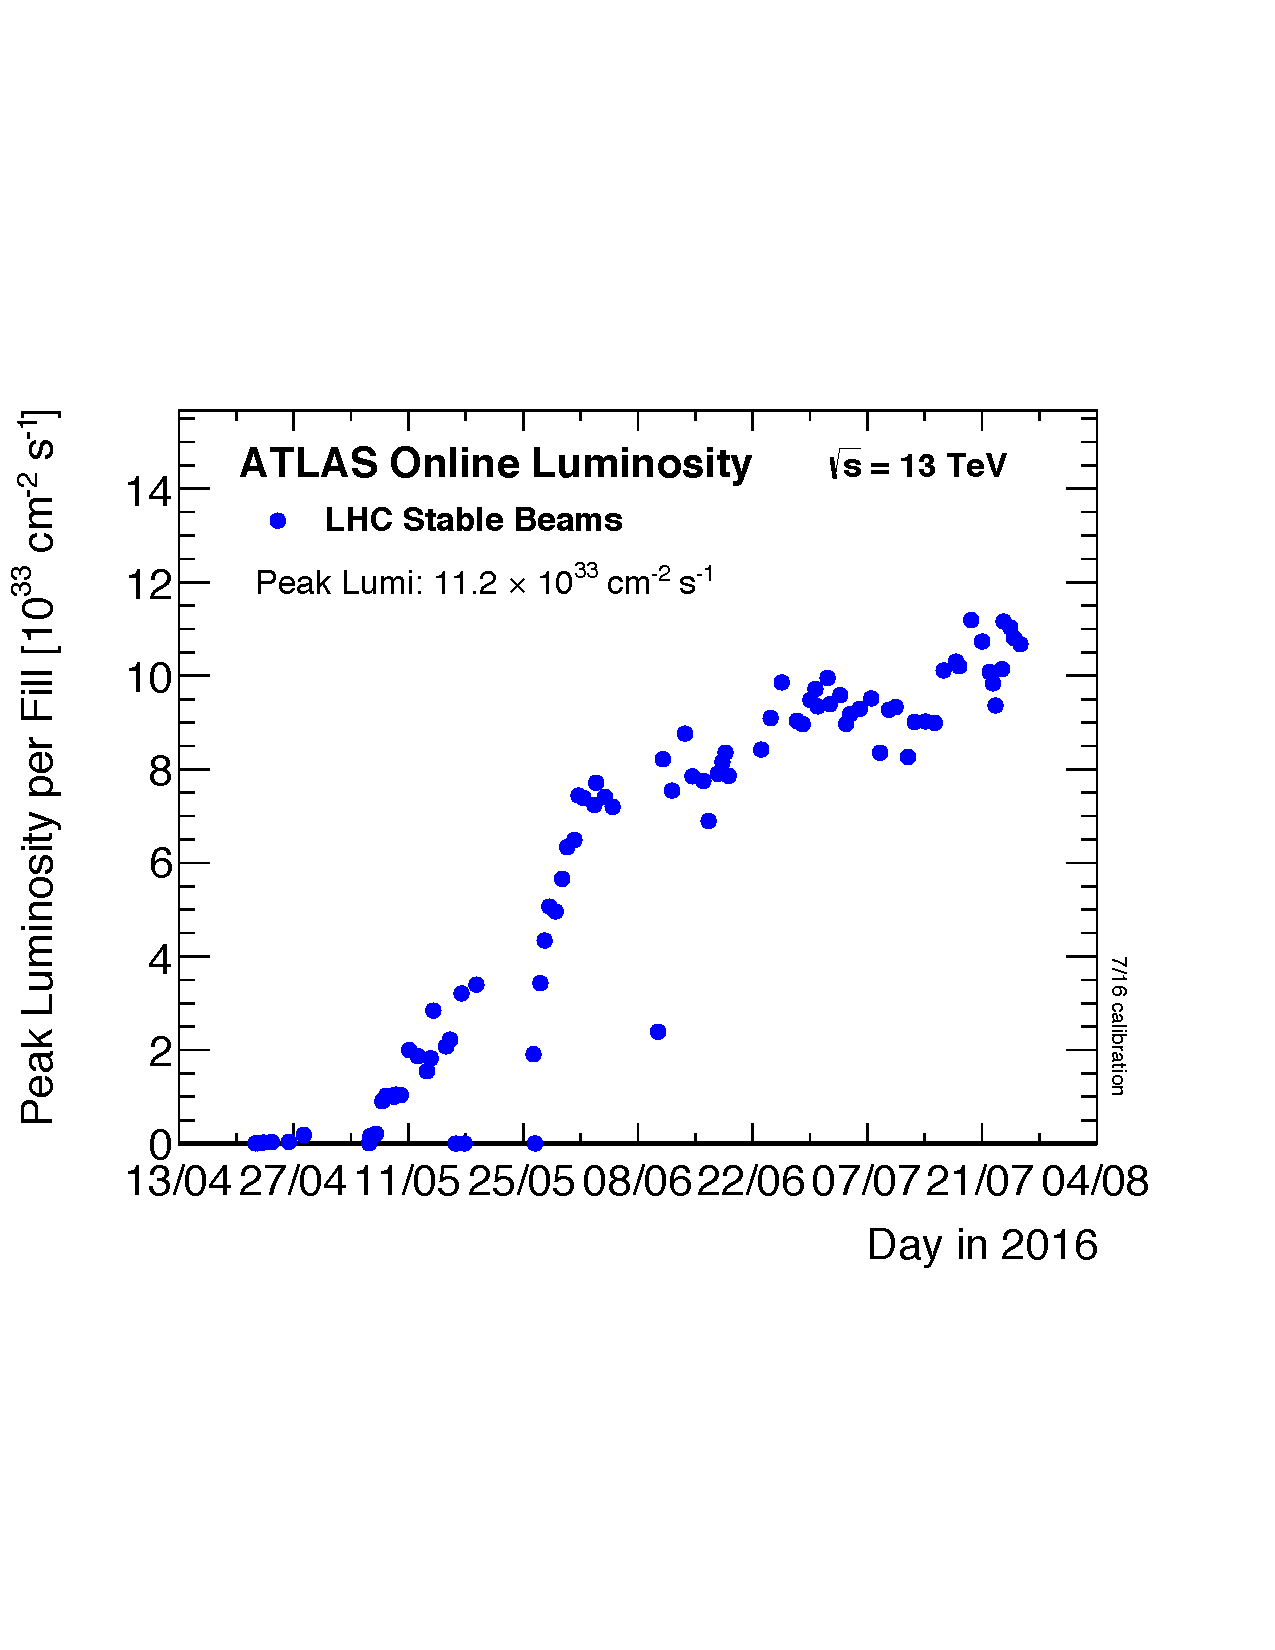
\includegraphics[width=\textwidth]{peakLumiByFill-1}
\end{subfigure}
\begin{subfigure}[t]{0.48\textwidth}
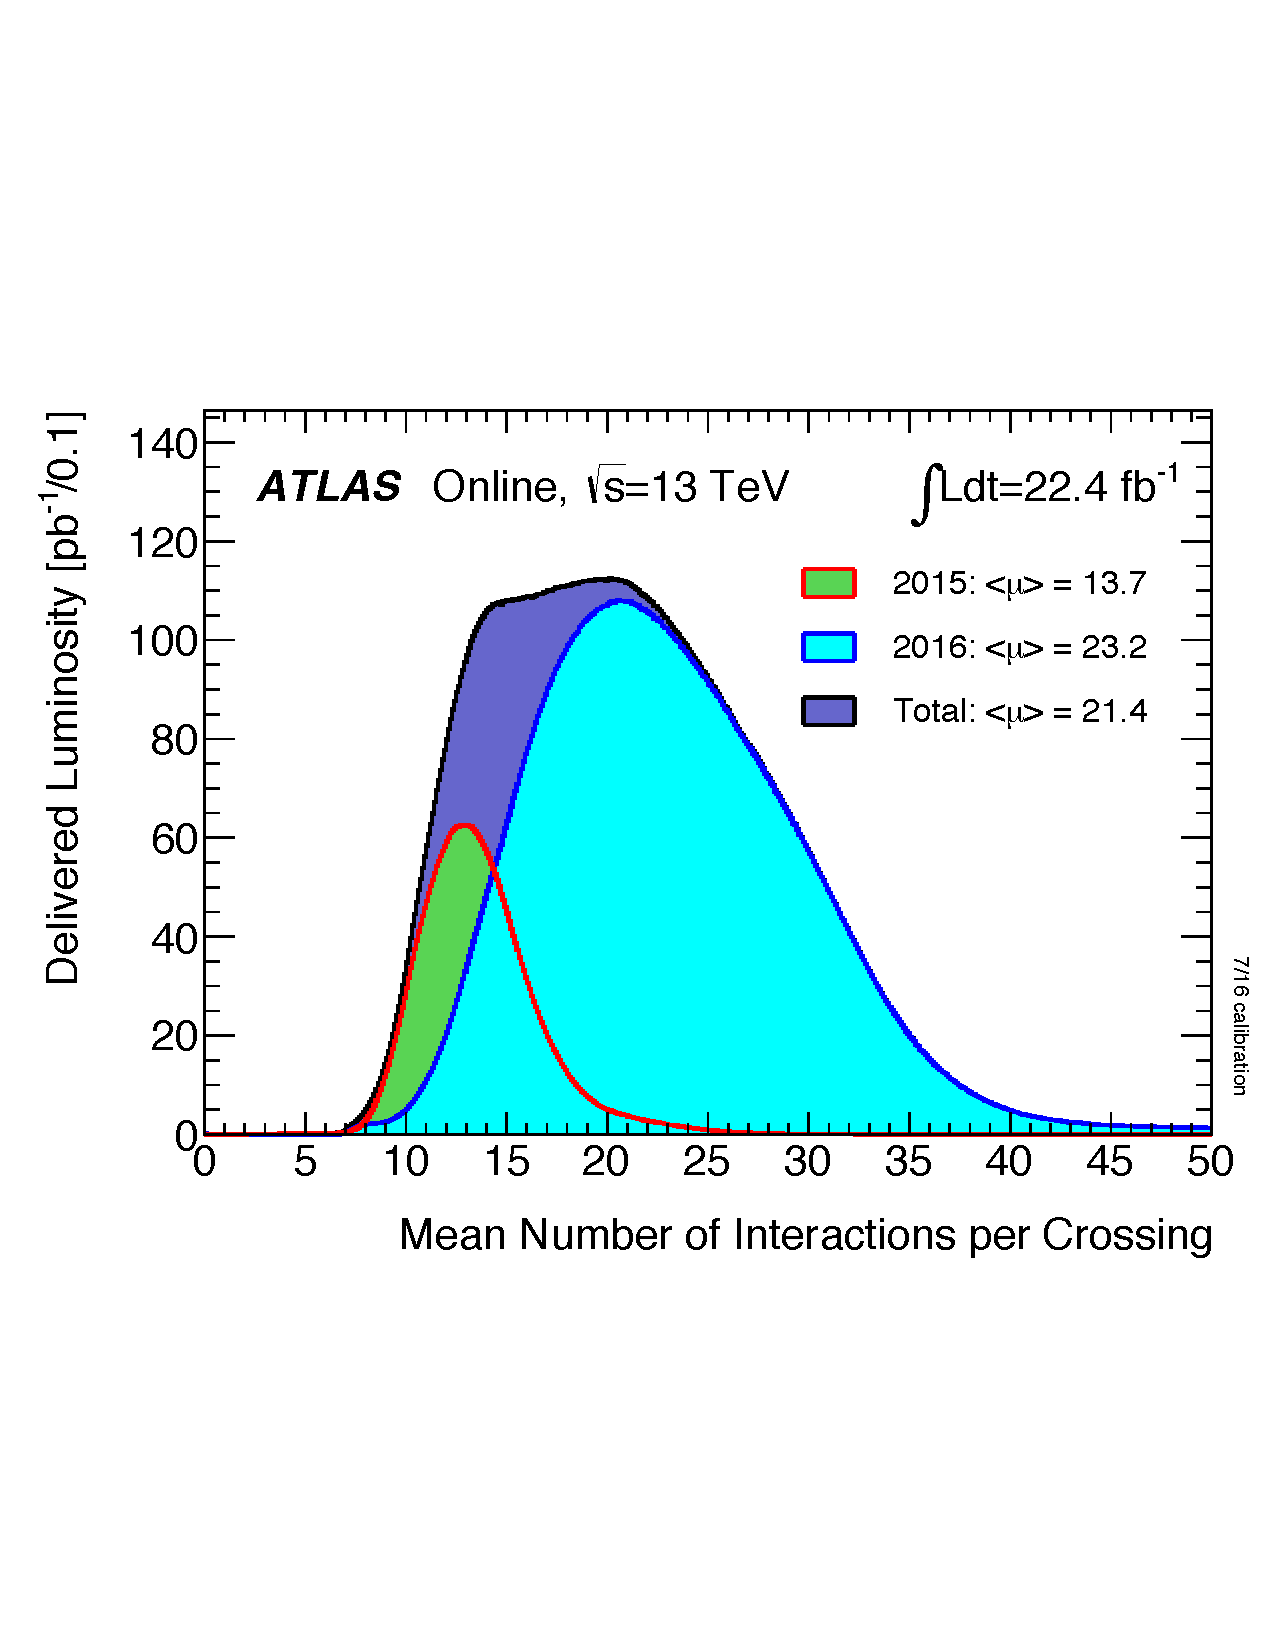
\includegraphics[width=\textwidth]{mu_2015_2016_ICHEP}
\end{subfigure}
\vspace{-2cm}
\caption{Run conditions during Run 2: ATLAS online luminosity (left), ATLAS online pileup (right) \cite{atlasTwiki}.}
\label{fig:lumi_pileup_1}
\end{figure} 
The L1 accept 
rate has also increased from 75 kHz in Run 1 to 100 kHz in Run 2 and the average output rate of the data logger system has 
increased from 400-600 Hz in Run 1 to about 3 kHz with 1.5 kHz for physics data. 
%of which is from the 1.5 kHz for an event size of 1.5 MB. 
Moreover, there were new detectors that were added in Run 2
(Insertable B-layer (IBL), L1 topological trigger, Fast Tracker (FTK))\cite{Aad:1602235} leading to 
an increase of 20\% in the number of readout channels. 
To be able to deliver more rate to the High Level Trigger (HLT), the upgrade also targeted the Readout System (ROS)\cite{PanduroVazquez2016939}. 
For the same reason the two level of the HLT system were collapsed into a single level which made the system more flexible 
 allowing for incremental data retrieval and analysis. 
The dataflow network system was re-designed to increase its capacity and simplify its architecture\cite{1742-6596-396-1-012033}.

%Given all these changes, the DAQ system needed an upgrade to satisfy the new requirements. In particular, the upgrade targeted the 
%replacement of the buffering hardware of the Readout System (ROS) to increase the readout rate \cite{PanduroVazquez2016939}, 
%the merging of the Region-of-Interest (RoI) 
%based selection with event building and filtering into a single process allowing incremental data collection and analysis in the 
%High Level Trigger (HLT), and a re-design of the network system connecting the ROS with the HLT to increase its capacity and simplify 
%its architecture \cite{1742-6596-396-1-012033}. 


\section{ATLAS Dataflow Design}

%The ATLAS data-taking proceeds in stages starting from the RoIs
%identified by the L1 triggers that are sent to the HLT for processing.
In Run 1, the farm was subdivided to several slices, with 
each slice managed by a dedicated supervisor. This layout has been 
dropped in favor of global management by a single farm master 
operating at 100 kHz referred to as the HLT supervisor (HLTSV). 
The Region of Interest Builder (RoIB) that assembles the RoIs
previously implemented on a VMEbus 
system is now integrated with the HLTSV and the RoI building done in software. 
%The architecture of the HLT has changed where the two levels of 
%the software trigger, known as Level 2 and the Event Filter, that were each 
%running on separate farms were merged into 
%a single farm with an increased number of available cores. 
The change in the HLT architecture from two to one level
required re-writing the HLT software and algorithms in such a way that 
each node in the farm can perform all processing steps. The handling of these
processing steps is done by a single Data Collection Manager (DCM) process 
running on each HLT node to manage the L1 RoIs, the dataflow 
between the ROS and the HLT processing units (HLTPU), 
the event building processes, and the data logging.
 In the new architecture, the computing resources are managed more efficiently
by balancing the utilization of all cluster nodes depending on the active HLT 
algorithms and by sharing the HLT code and services to reduce memory and 
resource usage. 

The dataflow network was simplified and upgraded to handle a larger data volume.
A single network is used for 
RoI based access from the ROS, event 
building in the HLT processing nodes, and sending data for logging. 
A 10 GbE connectivity has been adopted throughout  the dataflow system
resulting in a factor of four increase in bandwidth between the data loggers and
the permanent storage, and a 4$\times$10 GbE output from each ROS PC to the core routers. 
The HLTSV and the HLT racks are all connected directly to each of the two core routers via 
 2$\times$10 GbE connection. Each HLT rack is hosting up to 40 nodes connected by 2$\times$1 GbE to the top-rack switches. 
The capacity of the routers can accommodate
an increase in the number of HLT server racks and ROS PCs by a factor of two, 
which will be needed when the system scales as run conditions 
change. The core routers also provide load balancing and traffic shaping protocols \cite{1742-6596-396-1-012033}
to distribute the data throughout the system more evenly. A duplication of core routers provide link redundancy at every level in 
case of link or switch failures.


%\begin{figure}[t!]
%\centering
%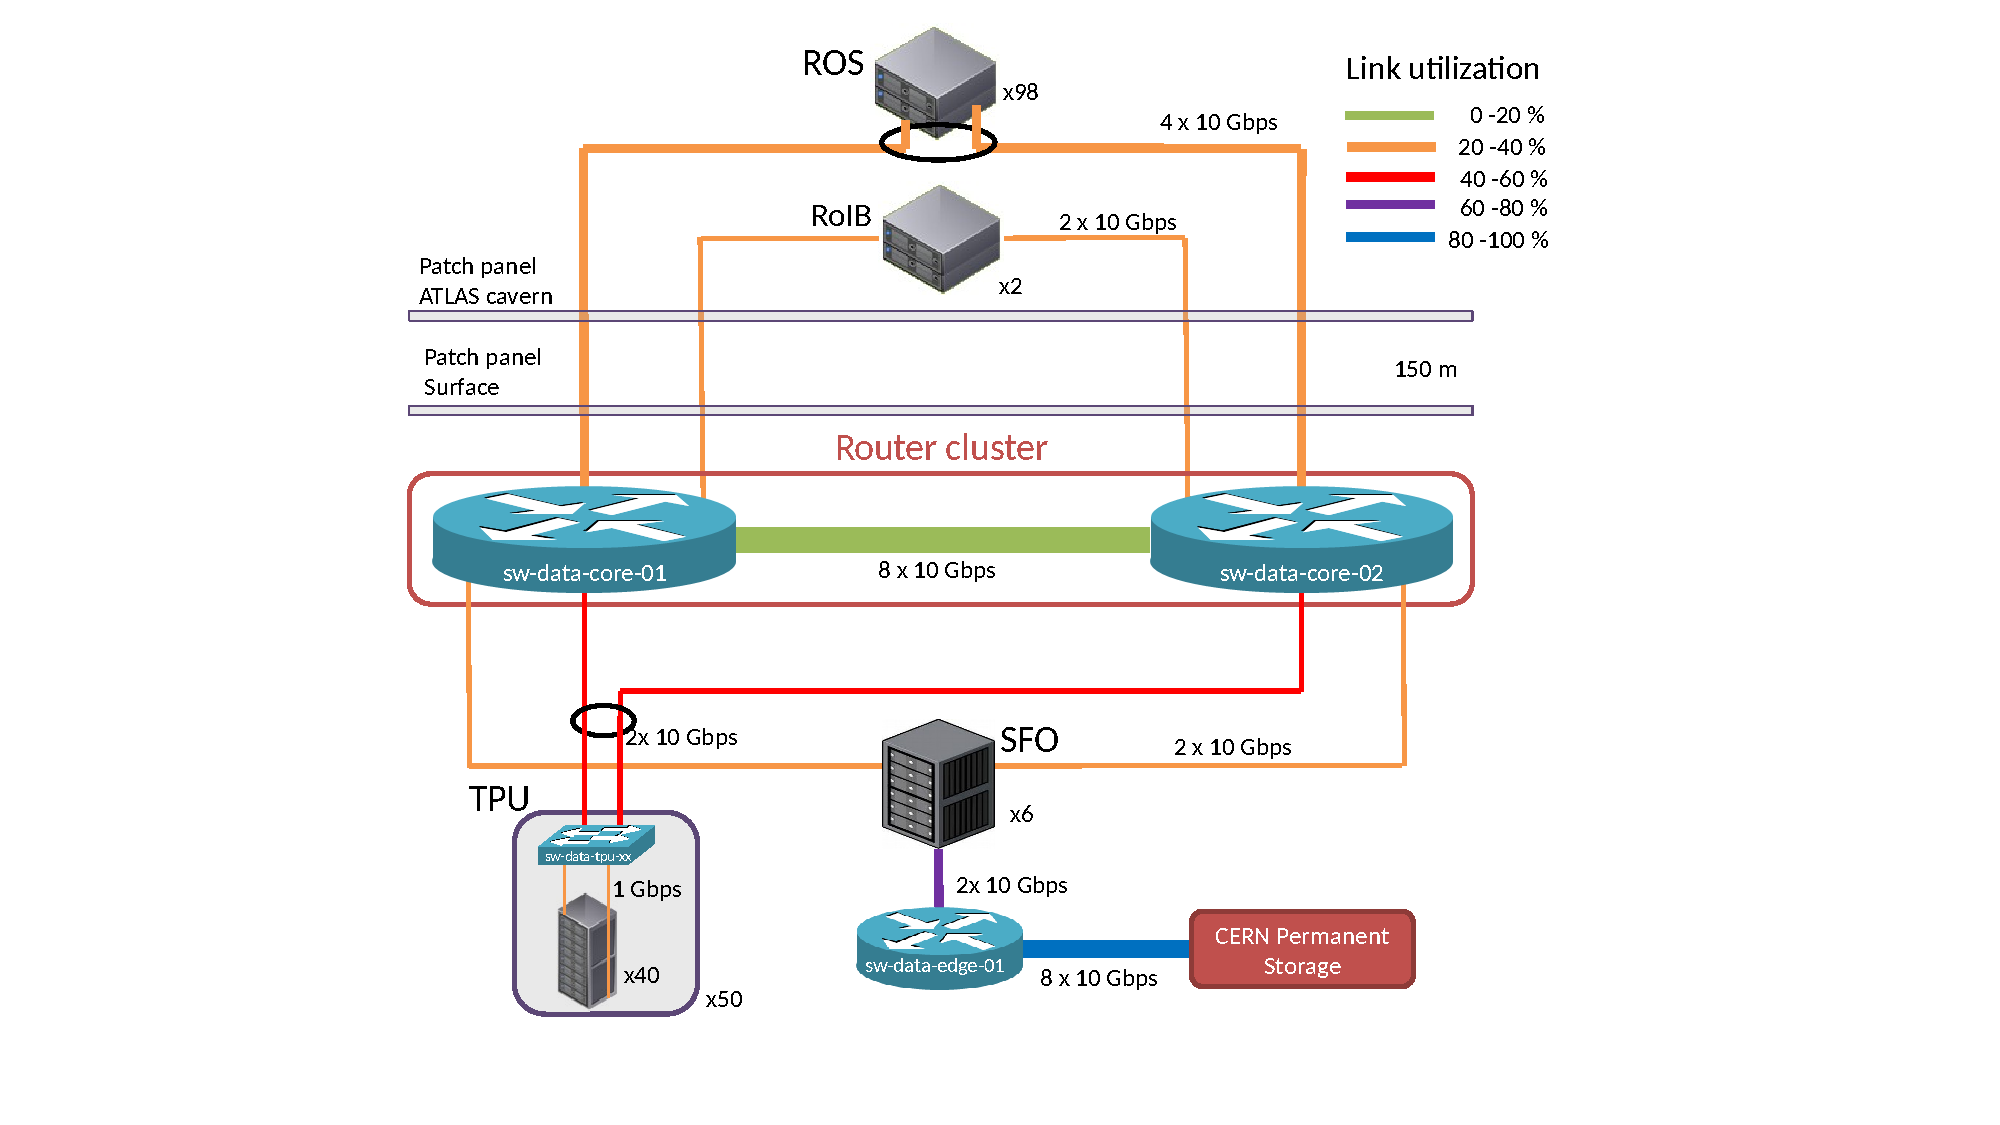
\includegraphics[width=1.2\textwidth]{network} 
%\vspace{-1cm}
%\caption{ATLAS Dataflow network}
%\label{fig:tdaq_diagram}
%\end{figure} 

To take advantage of multi-core architectures, the dataflow
 software is using multi-threaded software design for CPU consuming operations.
The Input/Output of the dataflow is based on asynchronous communication using industry standard libraries
such as the Boost::ASIO library. All the ATLAS software suite was switched to exclusively 64 bit operation in 2016.



%In summary, the elements of the Run 2 ATLAS dataflow are:

%\begin{itemize}
%\item The Readout Sytem (ROS) buffers front-end data from the detectors and provides a standard interface to the DAQ system.
%\item The Region of Interest Builder (RoIB) receives teh L1 trigger information from the RoIs and combines the information for the HLT supervsior.
%\item The HLT Supervisor (HLTSV) can handle the input from the RoIB and manage the HLT farm of about 2000 machines at over 100 kHz.
%\item The Data Collection Manager (DCM) handles all Input/Output on the HLT nodes, including RoI requests from the HLT and full event building.
%\item The HLT processing units (HLTPU) run the actualy HLT algorithms which 
%are forked from a single mother process to maximize memory sharing.
%\item The Data loggers or SubFarm Output (SFO) are responsible for savind the 
%accepted events to disk, and sending the files to CERN permanent storage infrastructure.
%\end{itemize}


\begin{figure}[!t]
\centering
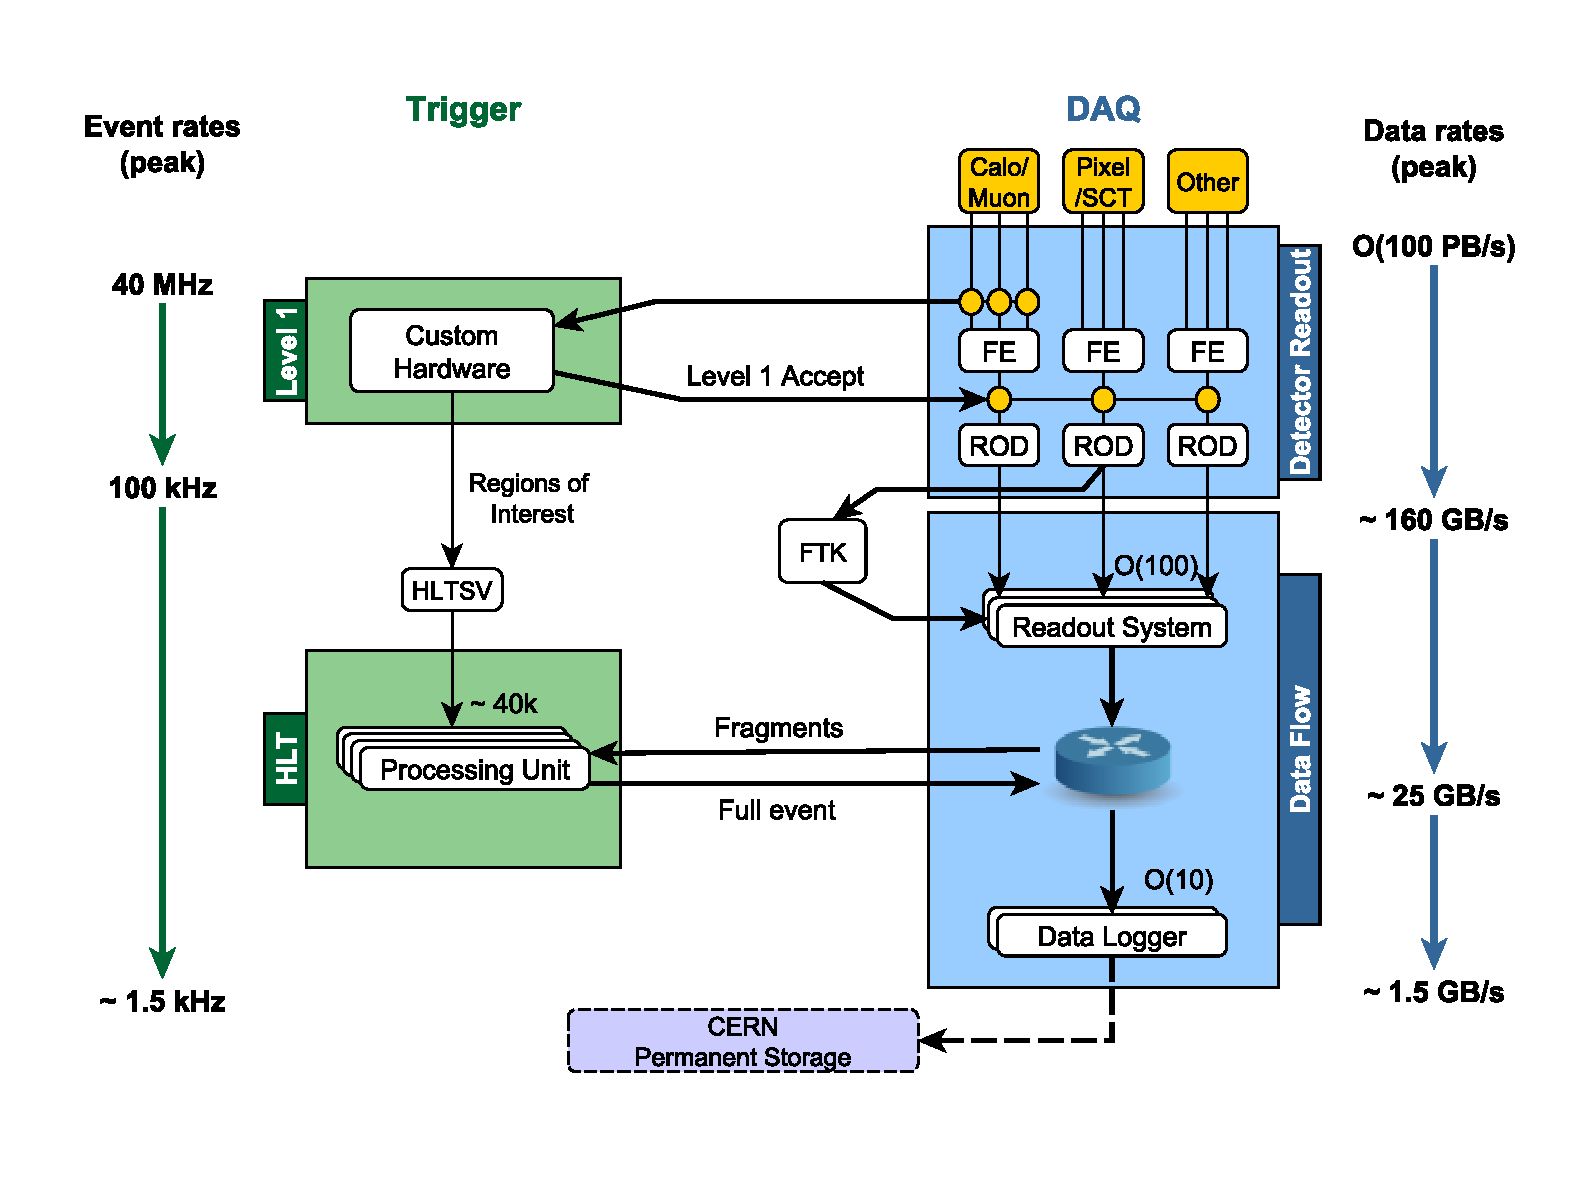
\includegraphics[width=0.75\textwidth]{tdaqFullNew2016}
\vspace{-0.5cm}
\caption{ATLAS TDAQ architecture.}
\label{fig:tdaq_diagram}
\end{figure} 

\section{Region of Interest Builder}

The first step of the HLT processing is to run on the RoIs found by the L1 hardware trigger. These
RoIs are collected and distributed to the HLT farm by the RoIB \cite{1748-0221-11-02-C02080} which was the 
latest change to the ATLAS dataflow. 
%This system was installed in ATLAS
% between the 2015 and 2016 data taking periods. 
The
evolution of the RoIB system from a crate of custom VME-based electronics (VME-RoIB) to a commodity
PC hosting a custom PCI-Express card (PC-RoIB) has been undertaken to increase the system performance,
flexibility, and ease of maintenance. The functionality of the VME-RoIB previously possible only in FPGAs has
now been implemented in a multi-threaded C++ software library. 
For each proton-proton collision that is accepted by the L1 trigger, the
RoIB receives an RoI record from the custom inputs via S-Link. The RoIB assembles these records into
a single record which is then forwarded to the HLTSV. The HLTSV then
distributes these single records to the HLT farm. The RoIB is also responsible for monitoring the
data integrity of the incoming fragments and diagnostic performance of the system.

As shown in Figure \ref{fig:roib_summary}, the performance of the PC-RoIB with realistic running ATLAS conditions
is improved over the VME-RoIB particularly at high RoI sizes. 

\begin{figure}[t!]
\centering
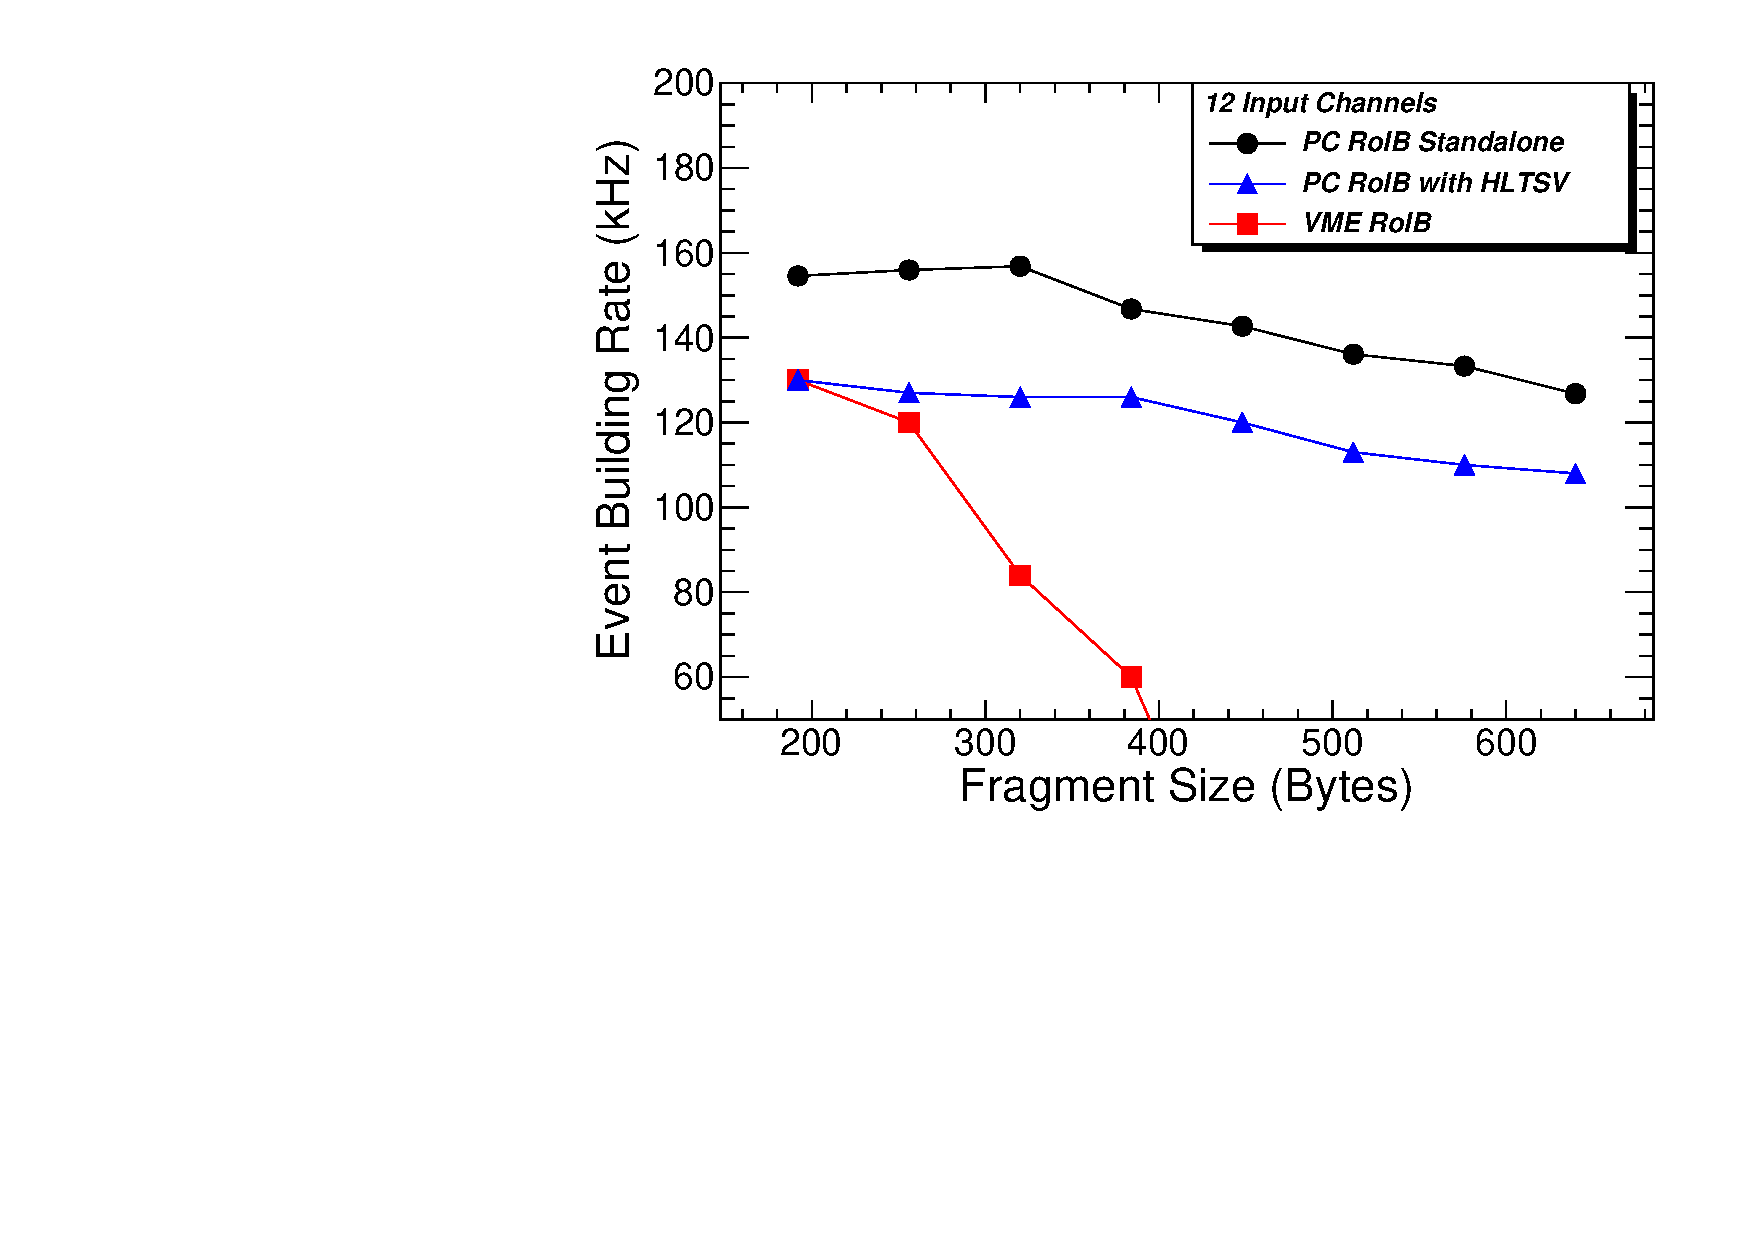
\includegraphics[width=0.5\textwidth]{roib_summary_size} 
\caption{The event building rate as a function of the RoI record size in Bytes. The rates are shown for a standalone application that implements 
a minimal interface for event building, the integrated RoIB software into an HLTSV process
running within the full ATLAS TDAQ software suite, and for comparison the VME-RoIB performance.}
\label{fig:roib_summary}
\end{figure} 

Figure \ref{fig:roib_pileup_l1rate} shows that the memory usage of the HLTSV is at the level of 5\% and that the RoIB event assembly does not depend 
on pileup conditions.


\begin{figure}[t!]
\centering
\begin{subfigure}[t]{0.48\textwidth}
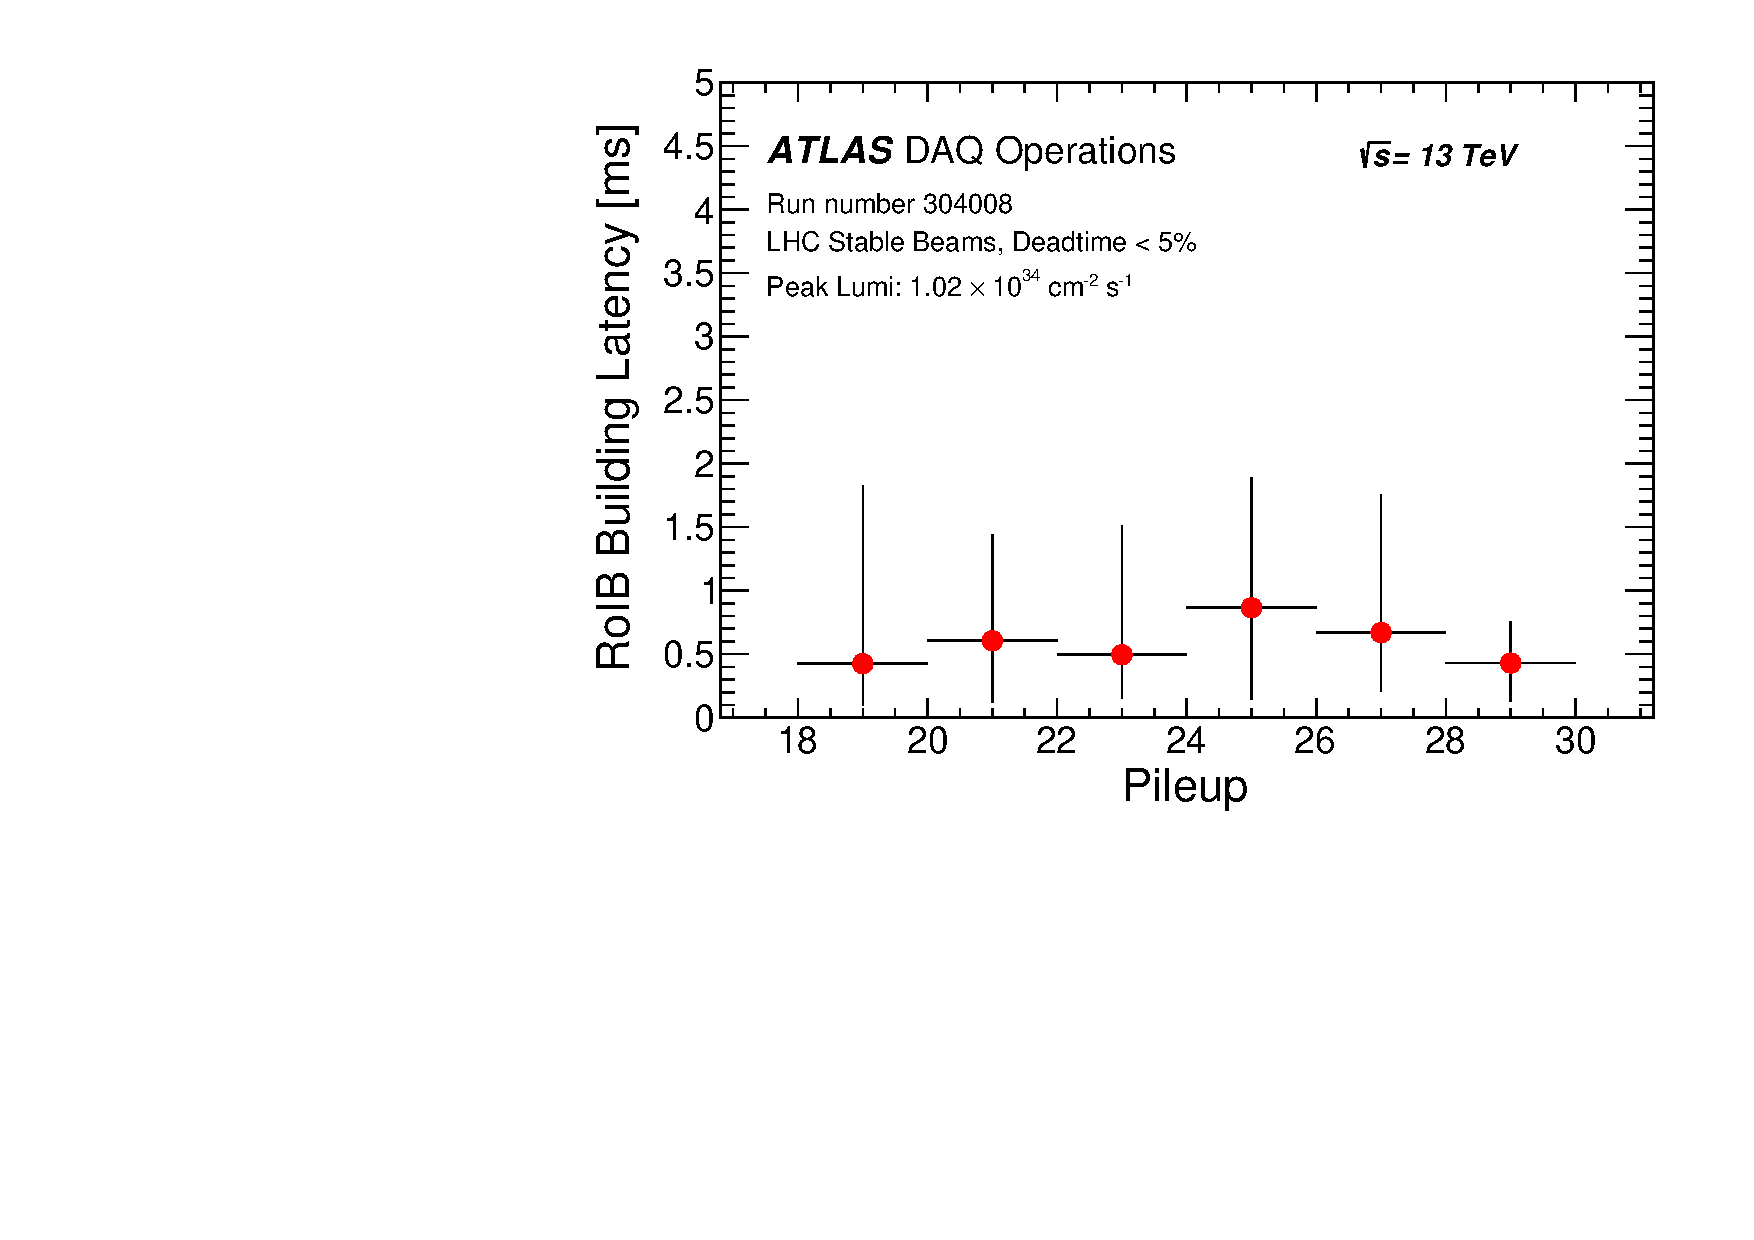
\includegraphics[width=0.95\textwidth]{GrAssym_run_304008_pileup_RoIBbuildtime}
\end{subfigure}
\begin{subfigure}[t]{0.48\textwidth}
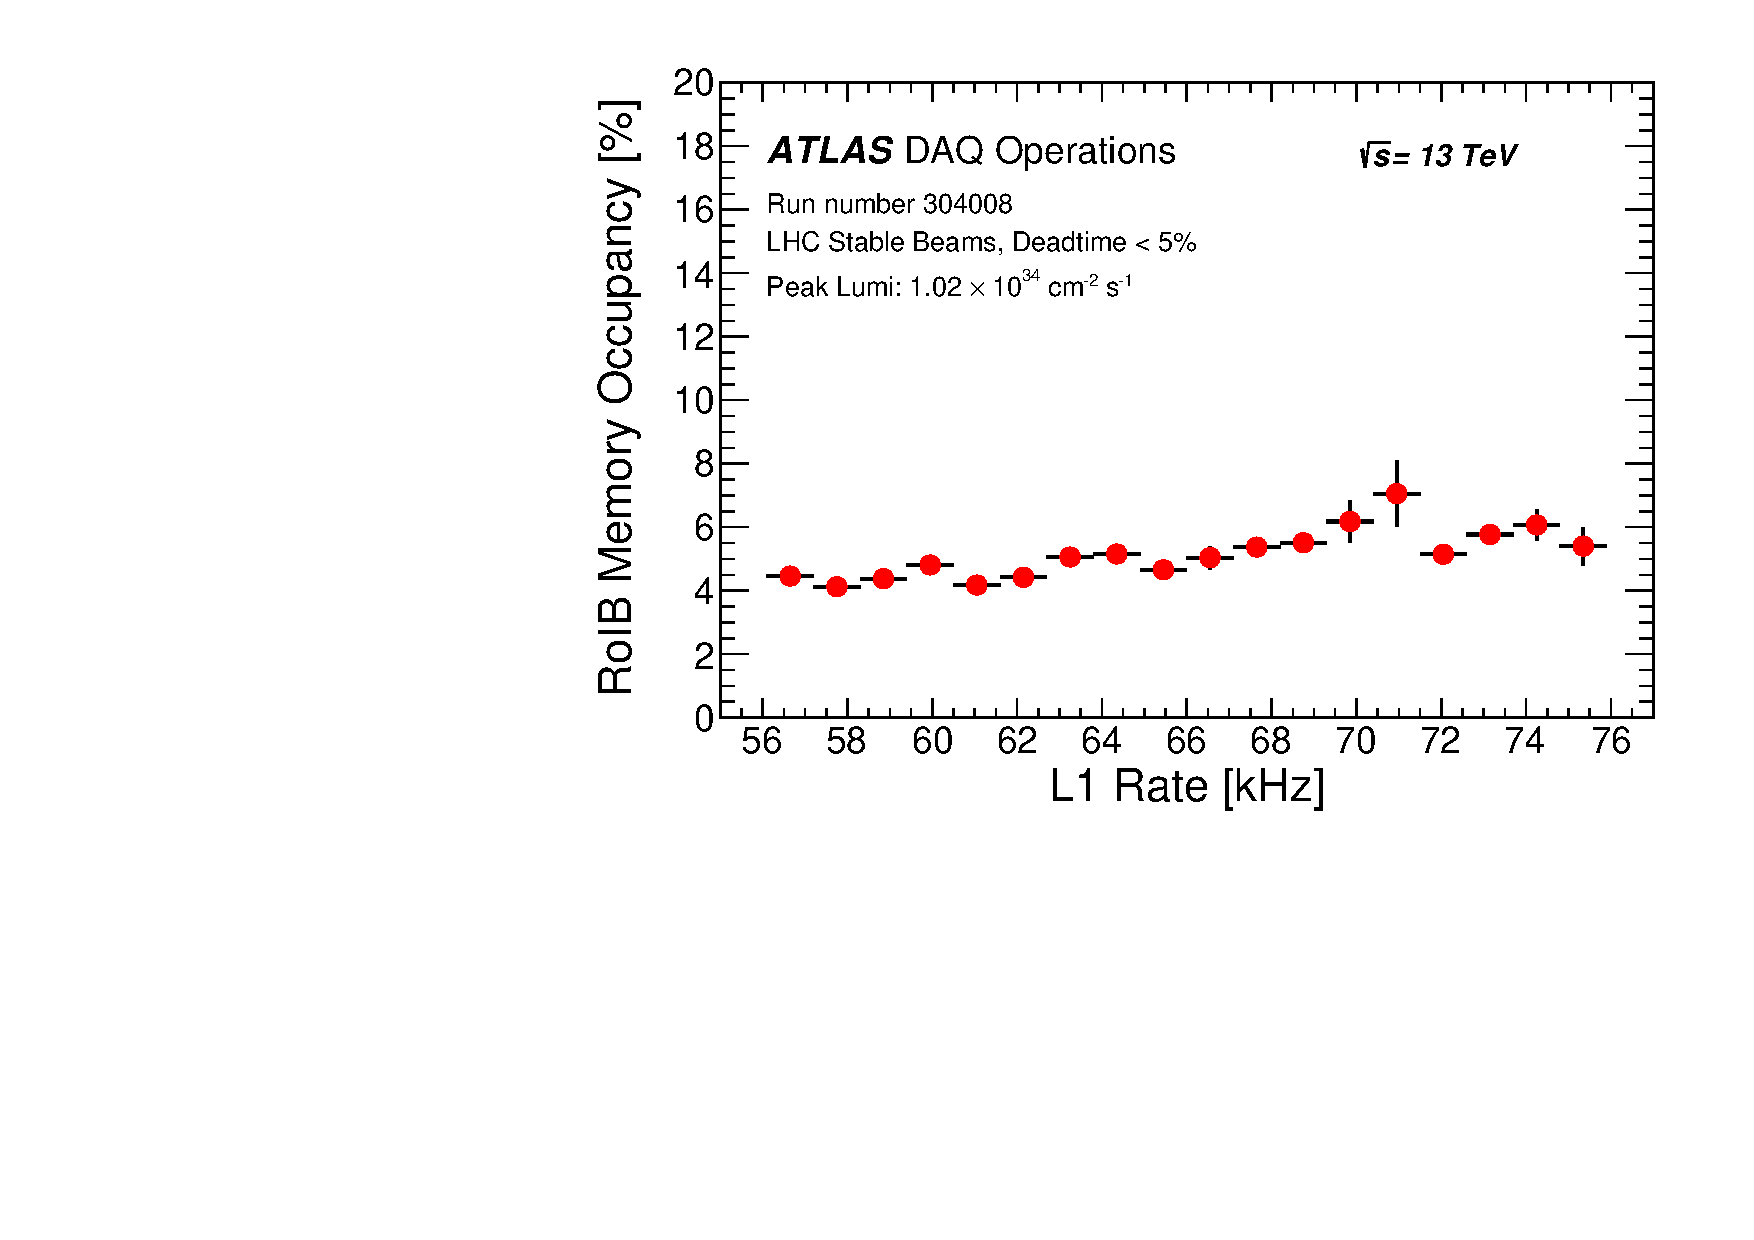
\includegraphics[width=0.95\textwidth]{hProf_run_304008_l1rate_RoIBMemOccup}
\end{subfigure}
\vspace{-0.25cm}
\caption{RoIB performance: RoIB building latency as a function of pileup (left), RoIB memory occupancy as a function of L1 rate (right).}
\label{fig:roib_pileup_l1rate}
\end{figure} 


%The initial tests were
%performed with a standalone application that implements a minimal interface for event building.
%Once the system was validated, the relevant code modules were integrated into an HLTSV process
%running within the full ATLAS TDAQ software suite with appropriately scaled test hardware to
%represent the remaining elements of the system.

%\section{Dataflow Network}

\section{Performance in Run 2}

The reliable operation of the TDAQ system directly impacts the efficiency of the ATLAS experiment 
in recording the collisions delivered by the LHC. As a result, high data-taking efficiency is crucial 
for the ATLAS physics program.
The ATLAS recorded efficiency in 2016 is over 90\%, as shown in Figure \ref{fig:tdaq_diagram} with a negligible fraction of data 
loss due to 
the DAQ system. The new dataflow architecture is scaling well with the increased 
instantaneous luminosity during 2016 data-taking and is capable of handling larger pileup and thus larger event sizes.
For illustration,  Figure \ref{fig:run_pileup} shows the evolution of the average processing time per event and 
the event size where there is relatively mild increase as a function of pileup which will within the system capacity.

\begin{figure}[t!]
\vspace{-0.5cm}
\centering
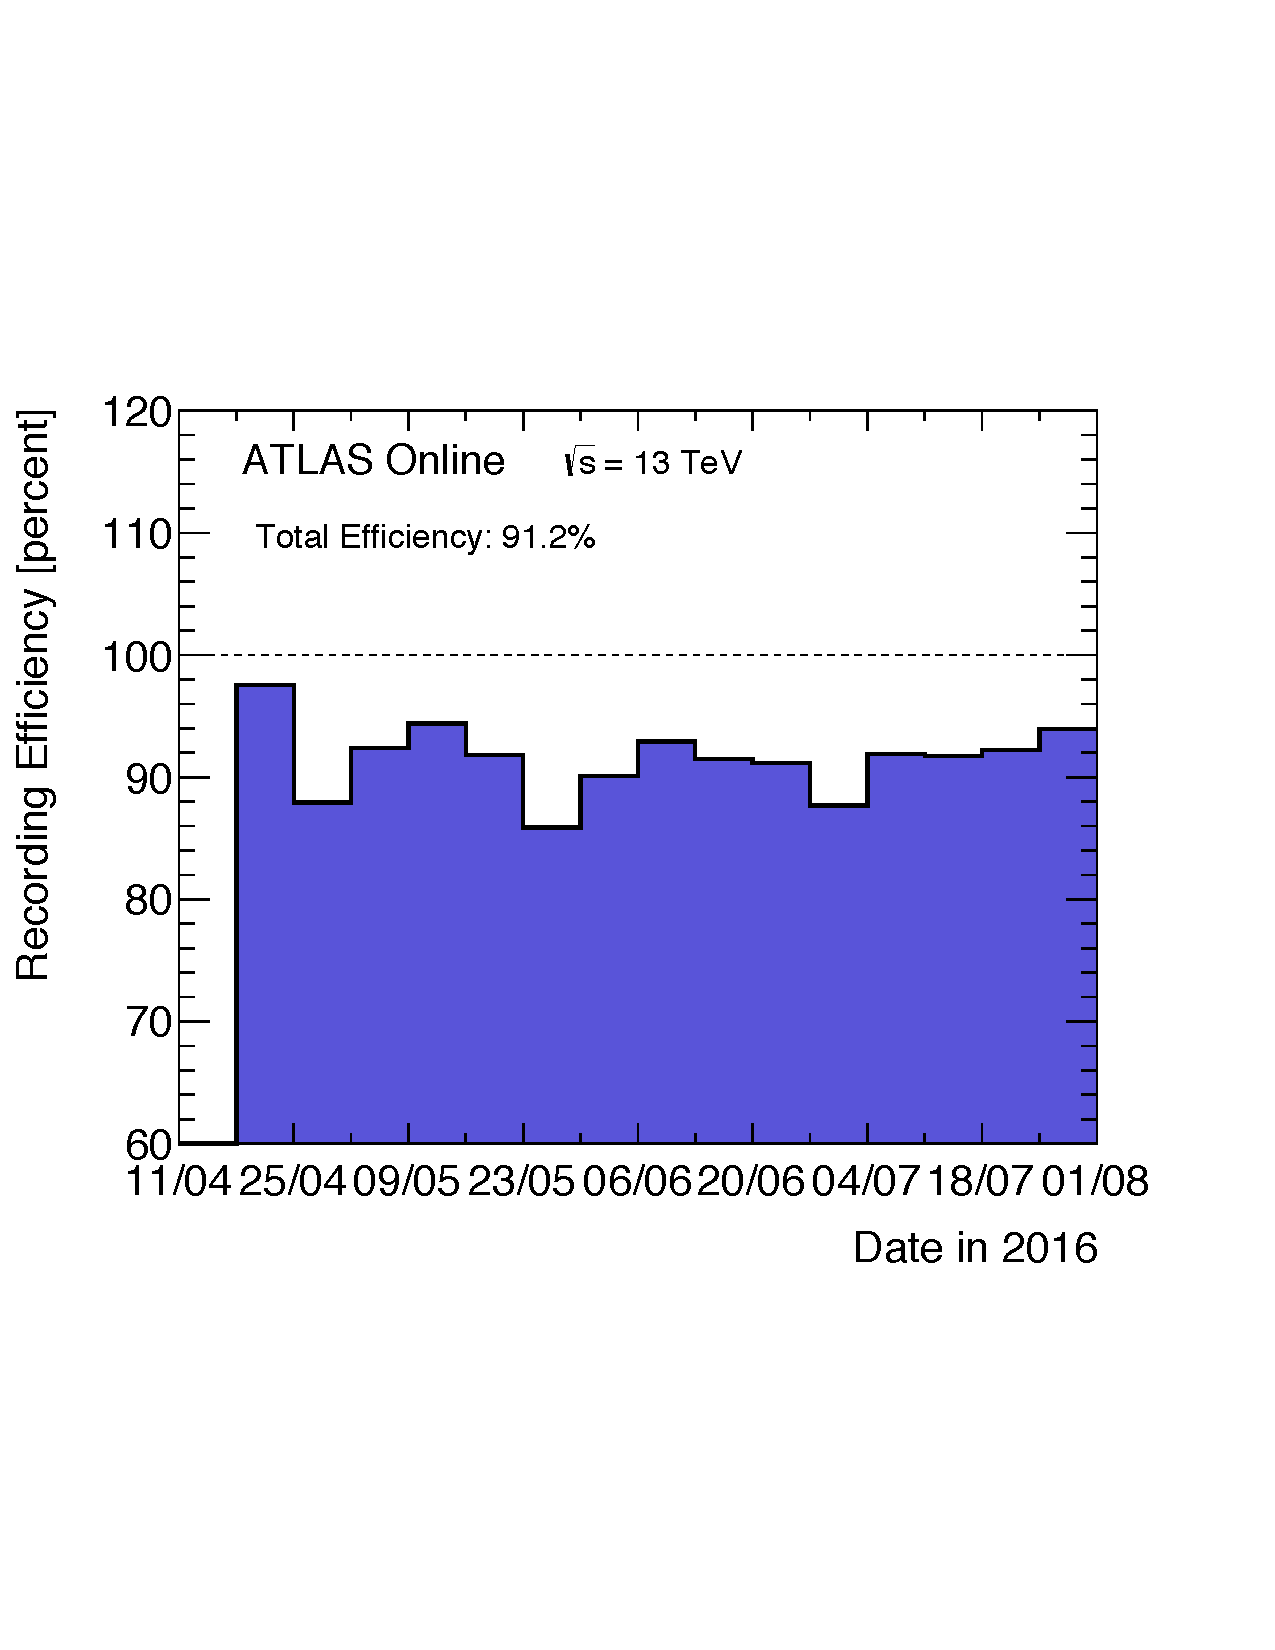
\includegraphics[width=0.5\textwidth]{recEffByWeek-1} 
\vspace{-2.5cm}
\caption{ATLAS recorded efficiency \cite{atlasTwiki}.}
\label{fig:tdaq_diagram}
\end{figure} 


\begin{figure}[t!]
%\vspace{-0.1cm}
\centering
\begin{subfigure}[t]{0.48\textwidth}
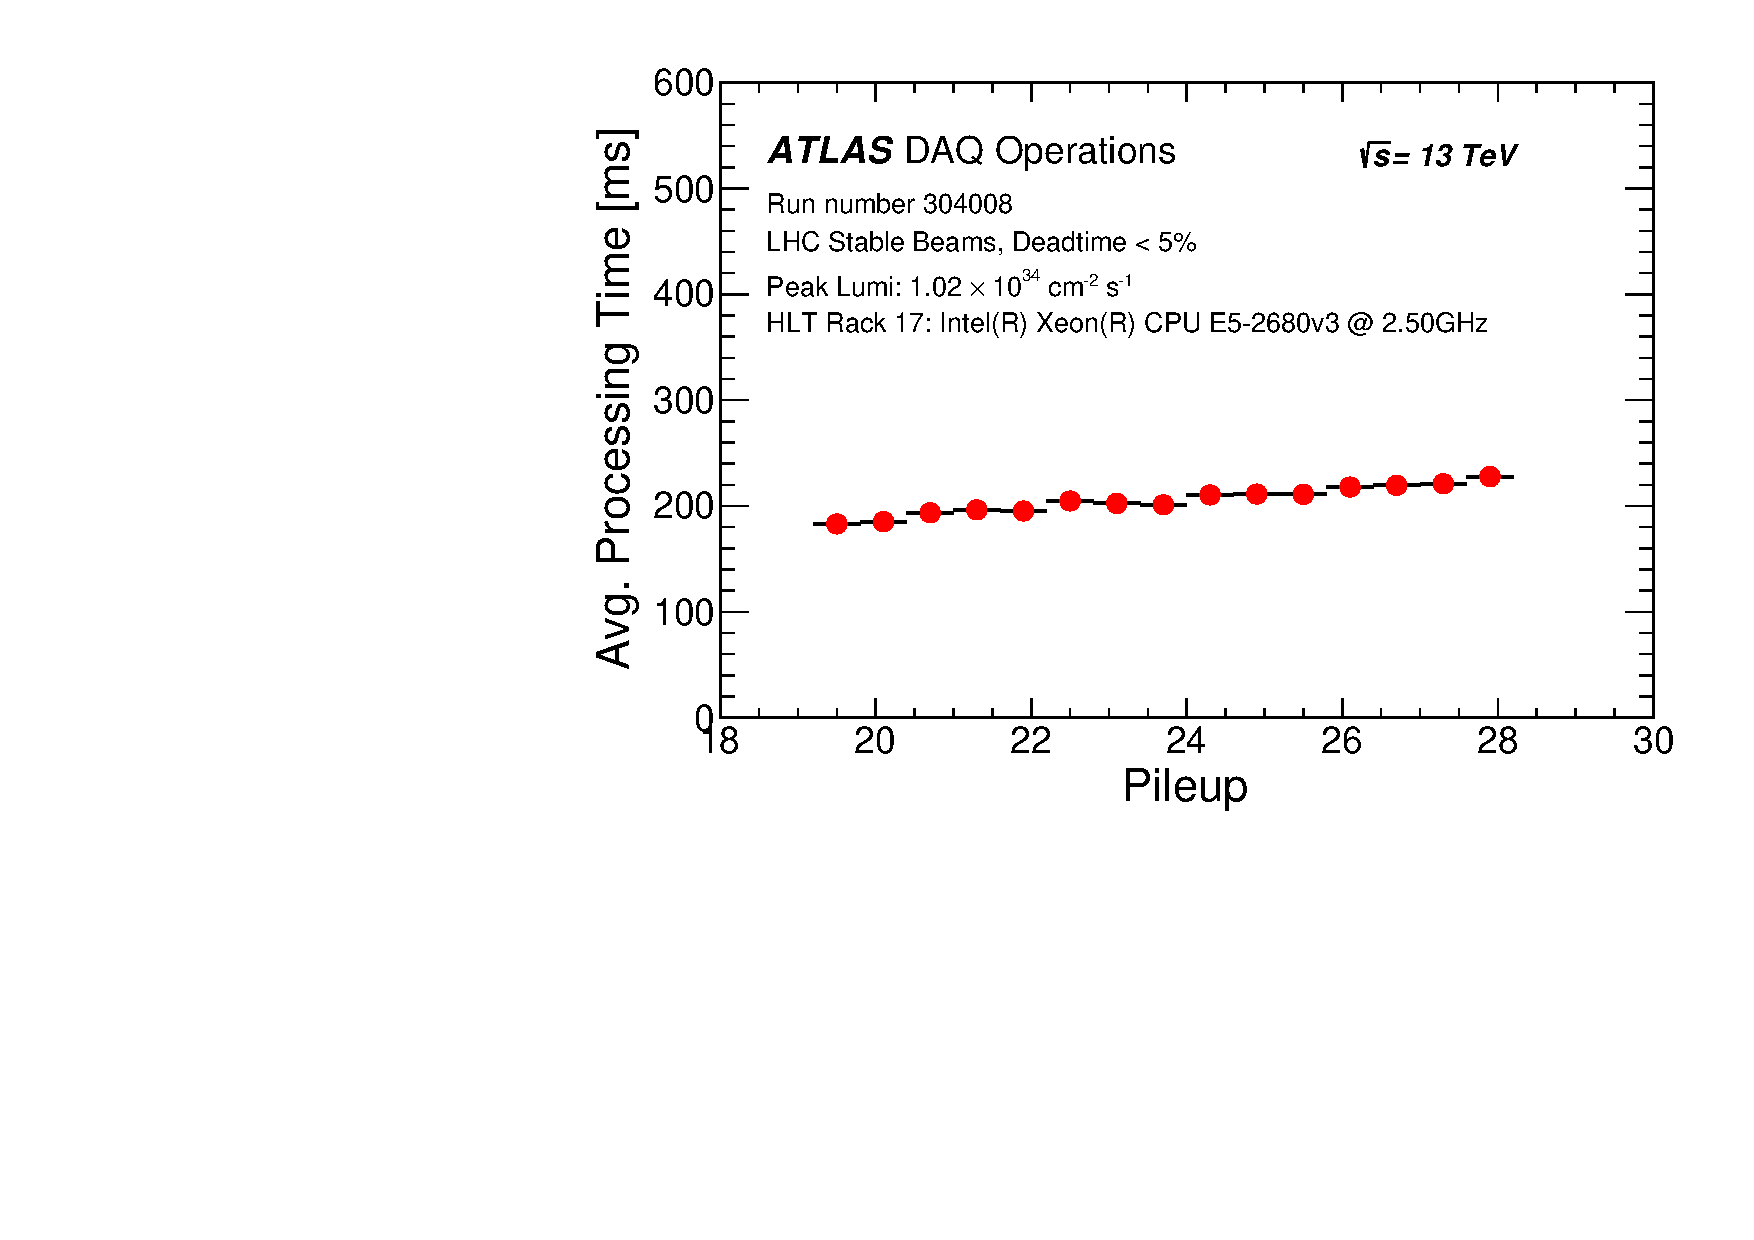
\includegraphics[width=.95\textwidth]{hProf_run_304008_pileup_AvgProcessingTime.pdf}
\end{subfigure}
\begin{subfigure}[t]{0.48\textwidth}
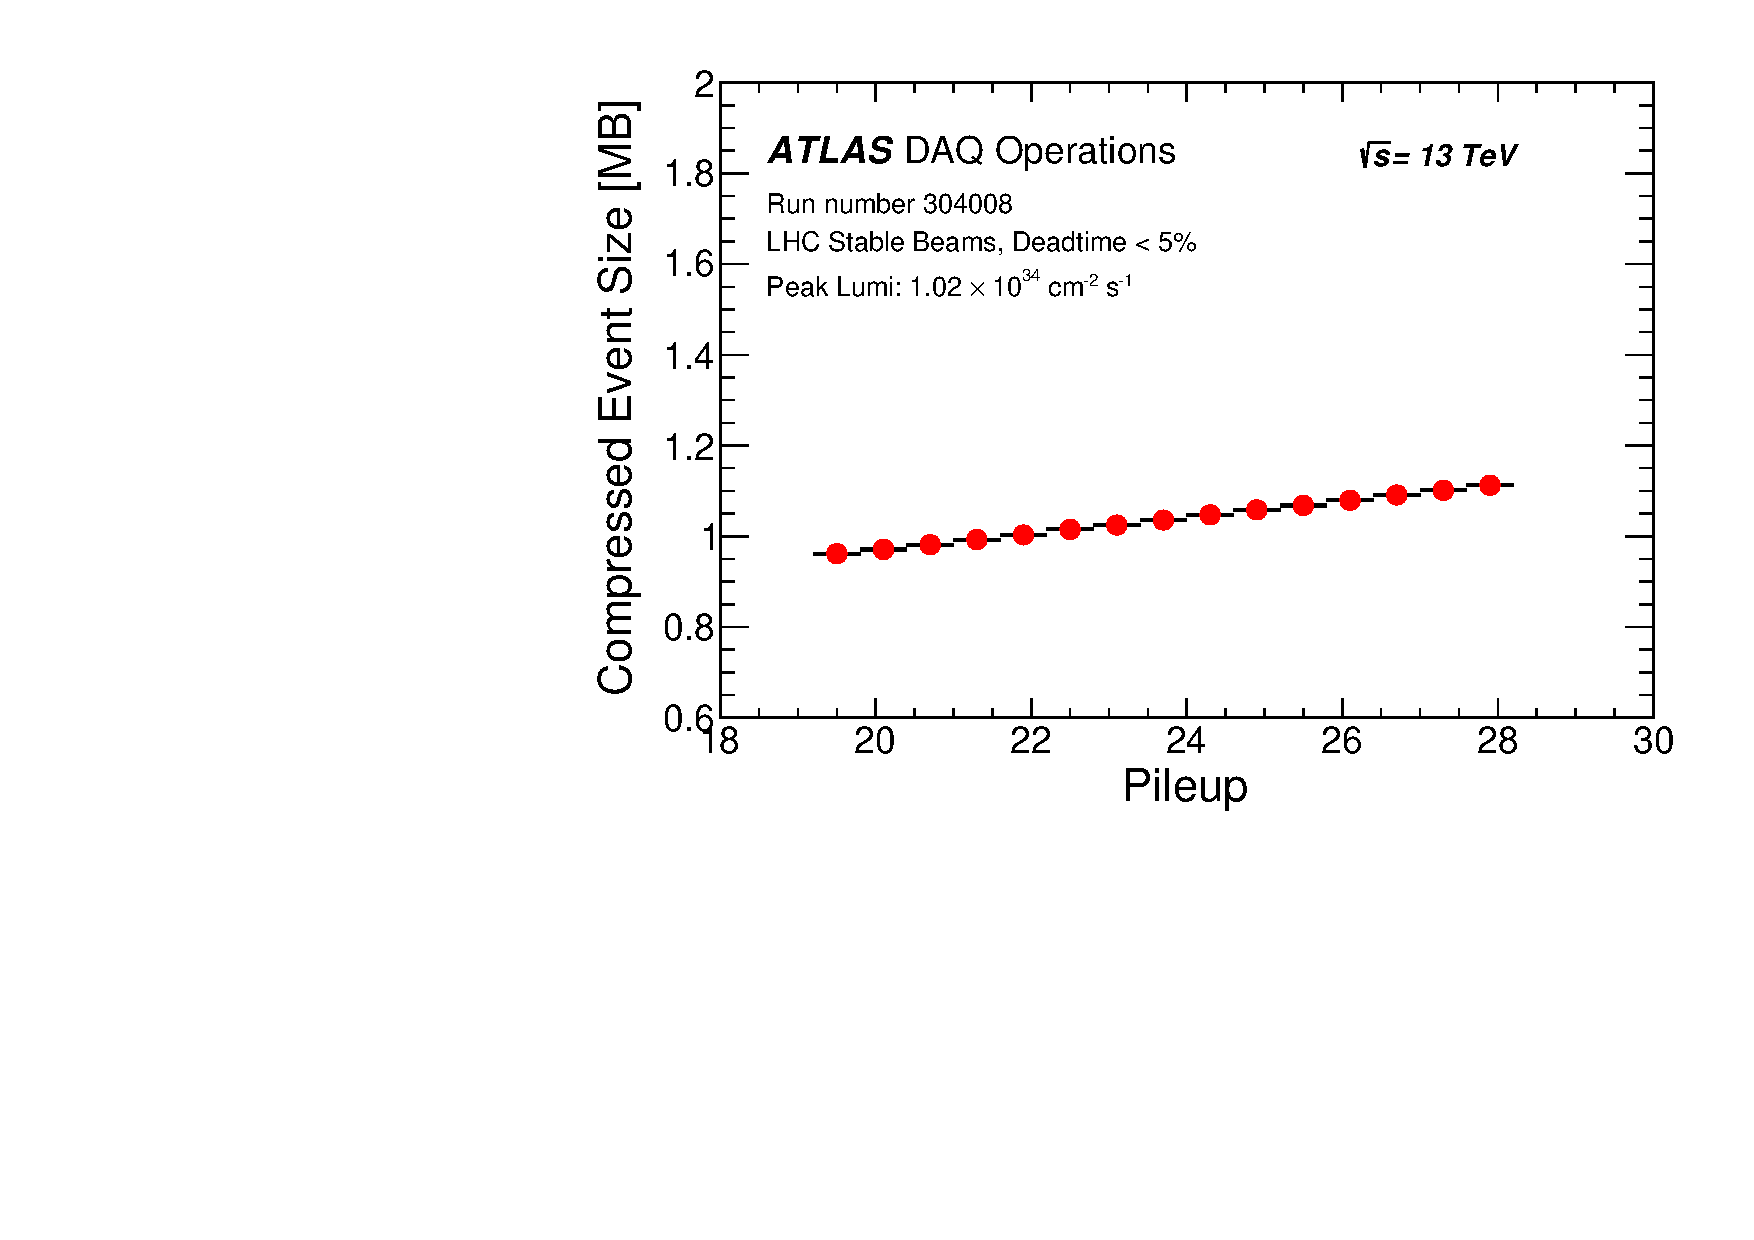
\includegraphics[width=.95\textwidth]{hProf_run_304008_pileup_EventSize.pdf}
\end{subfigure}
\vspace{-0.3cm}
\caption{Performance in Run 2: Average processing time as a function of pileup (left), compressed event size as a function of pileup (right).}
\label{fig:run_pileup}
\end{figure} 

\section{Conclusion}

The dataflow system of ATLAS was re-shaped for Run 2 in order to handle the 
 more demanding run conditions expected throughout the run. The new redesign 
profitted from the technological progress 
that took place in the last few years. As a result, the new system 
is considerably simplified, more performant, and scalable. Moreover,
there is more headroom in performance to cope with more challenging run conditions
of the LHC to ensure that ATLAS DAQ continues delivering physics data with high efficiency. 


\section{Introduction}\label{sec:intro}

The ATLAS \cite{atlas} detector's data acquisition system, illustrated in Figure \ref{fig:atlas_tdaq}, makes use of a multi-tiered trigger to reduce 
bandwidth from the LHC proton bunch crossing rate of 40 MHz
to the \\1 kHz written to disk \cite{evolution}. The first tier (Level-1 or L1) \cite{l1}, implemented in real time with custom electronics, 
makes an early event selection to determine if any objects of interest are present and reduces the data flow to 
100 kHz. The second tier, referred to as the High Level Trigger (HLT) \cite{hlt}, is implemented on a commodity computing cluster running custom triggering software. The HLT uses information from the
hardware based L1 system to guide the retrieval of information from the Readout System (ROS) \cite{ros}. 

Jet, electromagnetic and tau clusters, missing transverse momentum ($E_{\mathrm{T}}^{\mathrm{miss}}$), $\sum E_{\mathrm{T}}$, 
jet $E_{\mathrm{T}}$, and muon candidate information from L1 determine detector Regions of Interest (RoIs) that seed HLT processing. These RoIs are provided to the HLT by a custom VMEbus based system, referred to as the Region of Interest Builder (RoIB) \cite{vme_roib}.
The RoIB collects data from L1 
trigger sources and assembles the data fragments into a complete record of L1 RoIs. These RoIs are made available to the HLT to initiate event processing. In order to improve maintainability and scalability, and to minimize the amount of custom hardware needing to be supported, 
the RoIB will be implemented using commodity server hardware and an interface technology already deployed 
within the ATLAS Trigger and Data Acquisition (TDAQ) system. The approach of implementing the RoIB functionality in software has been investigated in the past 
and the conclusion at that time was that a software based approach is possible but requires a higher rate readout card \cite{swroib_past}. 
Since data readout cards operating at high rates became available and the capabilities of computers have improved with the increase 
in CPU clock speed and number of cores, it became possible to implement the RoIB functionality using a PC based approach. 
The PC based RoIB must duplicate the functionality of the VMEbus based RoIB which means that the PC based solution must receive and assemble the
individual L1 fragments, and pass them as a single L1 result to the HLT. Modern computers have multicore CPU architectures 
with the possibility of running multi-threaded application, a feature which is being fully exploited in the RoIB software to achieve 
the desired performance of 100 kHz over 12 input links for fragment sizes of 400 bytes.  
This paper describes the evolution of the RoIB from the VMEbus based system to the PC based system and gives details on the hardware, 
firmware, and software designs used to achieve the full RoIB functionality. 



\begin{figure}[tbp] % figures (and tables) should go top or bottom of
                    % the page where they are first cited or in
                    % subsequent pages
\centering
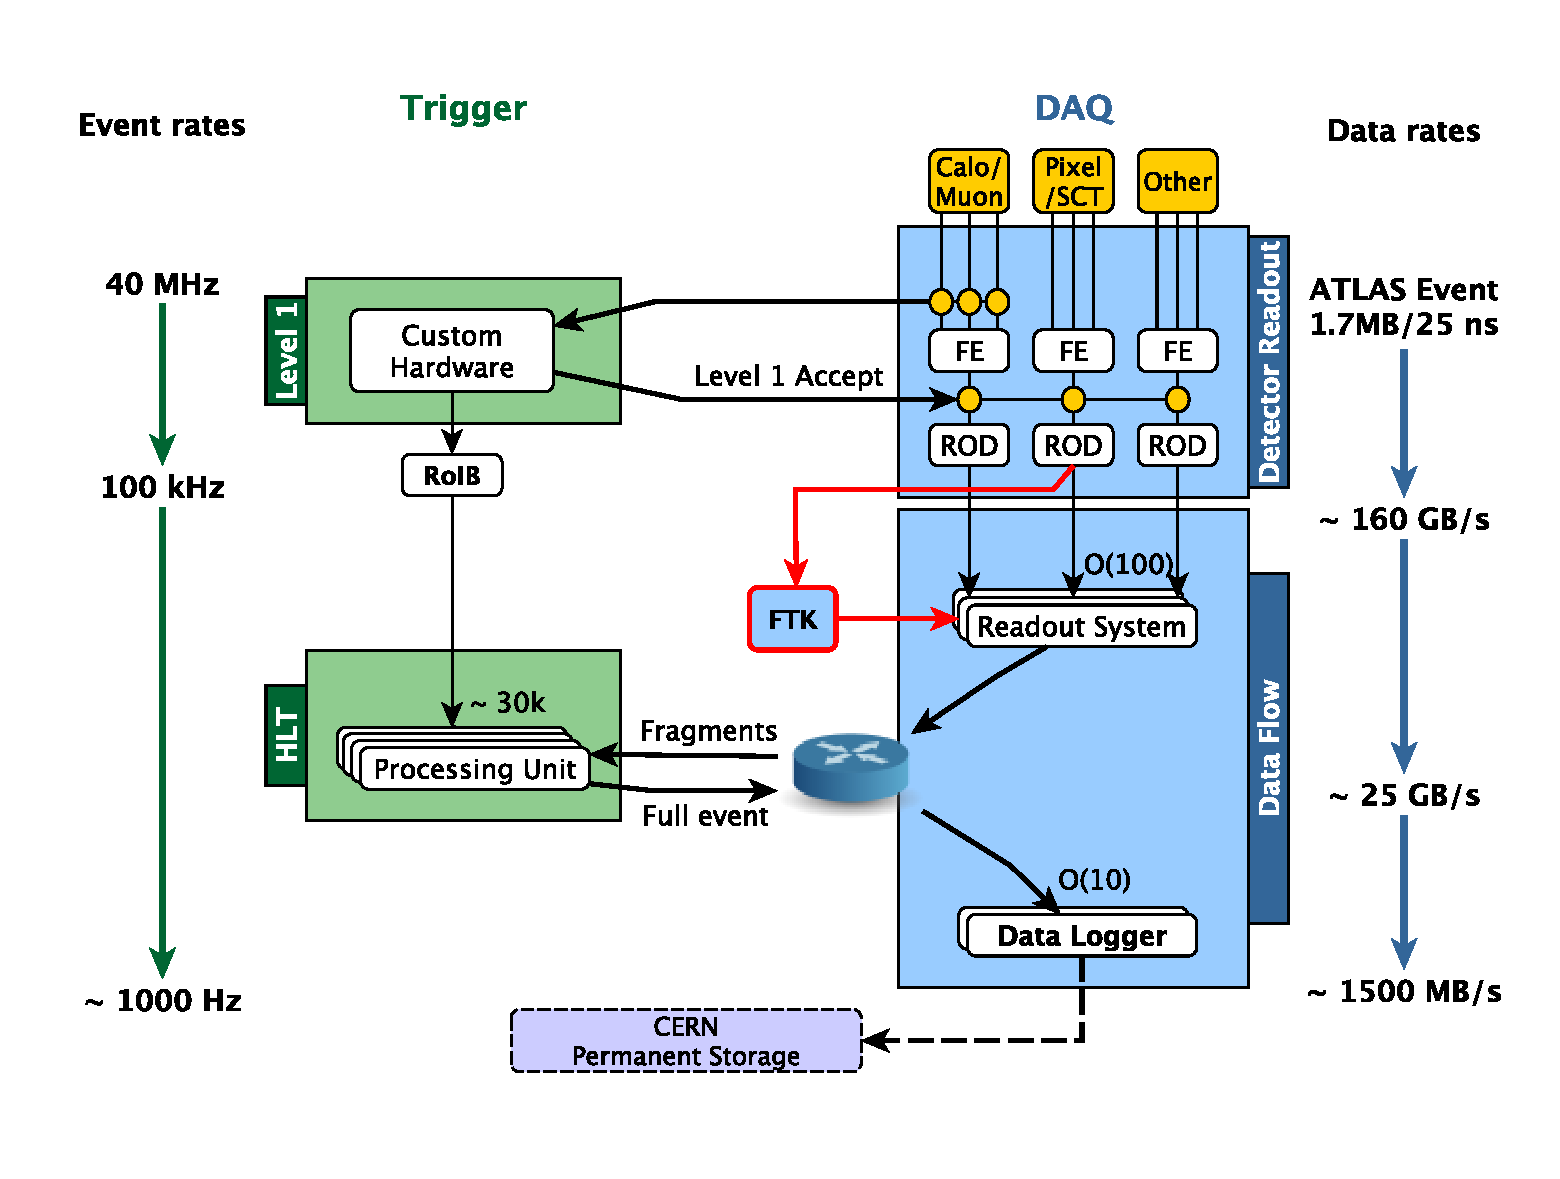
\includegraphics[width=.9\textwidth]{tdaqFullNew2015}
\caption{ATLAS TDAQ Architecture.}
\label{fig:atlas_tdaq}
\end{figure}



%\section{ATLAS TDAQ System }\label{sec:tdaq}

%\subsection{Challenges}\label{sec:tdaq_chal}

%\subsection{Architecture}\label{sec:tdaq_archi}


\section{VMEbus based RoIB}\label{sec:roib}

\subsection{Hardware implementation}\label{sec:roib_current}

The RoIB is implemented as a custom 9U VMEbus system that includes a controller which configures and monitors the system along with custom cards 
that receive and assemble the event fragments and send them to the HLT. Figure \ref{roib_run1} shows a block of the RoIB and 
its connection to external systems.
%\footnote{Note the L2 Supervisor farm from Run-1 has evolved to a commodity server PC running the HLTSV application.}.

\begin{figure}[tbp] % figures (and tables) should go top or bottom of
                    % the page where they are first cited or in
                    % subsequent pages
\centering
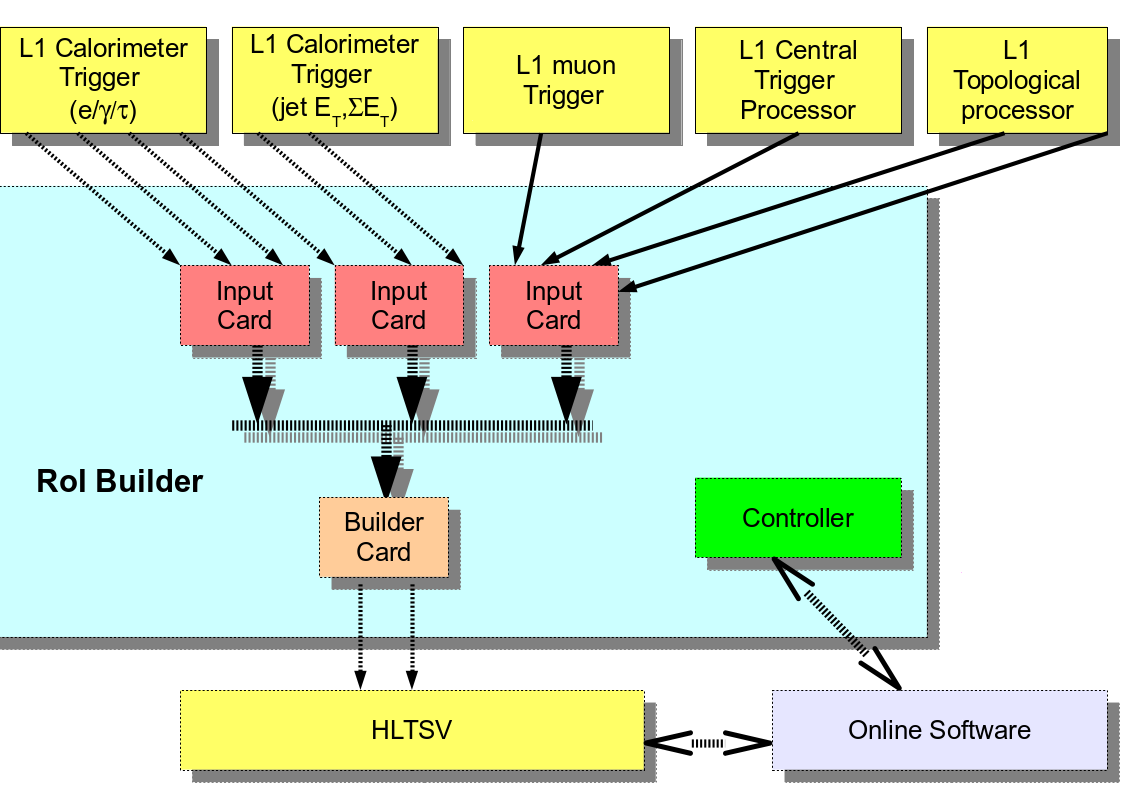
\includegraphics[width=.65\textwidth]{RoIB_context_v2.png}
\caption{Block scheme of the RoI Builder and overview of connections to external systems.  The
custom input and builder cards and the controller, a commercially available single board computer,
are installed in a single 9U VMEbus crate. The controller connects to the Control Network to interact with the rest of the 
data acquisition system.}
\label{roib_run1}
\end{figure}

The RoIB contains four input cards and uses one builder card in the Run-2 configuration. Each input card accepts three inputs from 
L1 subsystems. 
The builder card assembles the input data of the events and passes the results via two optical links 
to another receiver card in a PC running the HLT supervisor (HLTSV) application. The receiver card in the HLTSV is a TILAR card \cite{tilar}
 that implements four PCIe Gen1 lanes to interface with the two optical links. The HLTSV manages the HLT processing farm by using L1 results provided by the RoIB, retrieves events from the ROS, assigns events to HLT farm nodes, and handles event bookkeeping including requesting removal of data from ROS storage when no longer required. 

The fragments received by the RoIB are identified by a 32 bit identifier, the extended L1 ID (L1ID). 
The RoIB input cards use the L1ID and the number of outputs enabled to assign keys to the various fragments and send them to the output channel in the builder card that was 
assigned that key value. The input data is transferred over a custom J3 backplane. The backplane operates at 20 MHz and transfers 16 data bits per 
clock cycle simultaneously for up to 12 inputs. The total maximum data throughput is therefore 480 MB/s, 40 MB/s per input.  
The maximum size of any single fragment is limited to 512 bytes imposed by resources available in the FPGA firmware. The current RoIB input 
links are listed in Table \ref{tab:roib_links}.

\begin{table}[tbp]
\caption{L1 input sources to the RoIB.}
\label{tab:roib_links}
\smallskip
\centering
\begin{tabular}{|c|c|}
\hline
Source & Links\\
\hline
Central Trigger Processor (CTP)  & 1  \\
L1 calorimeters (e/$\gamma$, $\tau$, jet, $\sum E_\mathrm{T}$) & 6  \\
Muon Trigger to CTP Interface (MUCTPI) & 1  \\
Topological processor (L1Topo) & 2  \\
Spare & 2 \\
\hline
\end{tabular}
\end{table}

\subsection{System Performance and Evolution}\label{sec:roib_limit}

The custom VMEbus based RoIB operated reliably during the first run of the LHC, however, it is desirable to have a more flexible RoIB. 
In addition, the RoIB is getting close to its design limitation, as seen 
in Figure \ref{fig:cern_robinnproib}. For fragments of 400 bytes and inputs from eight L1 systems, referred to as channels, the current RoIB rate limit is 60 kHz which is below the required 100 kHz at 
L1. While the current fragment size coming from L1 are around 160 bytes, the sizes are expected to grow due to the increase of instantaneous 
luminosity and the complexity of L1 triggers. The current VMEbus system will be replaced by a PCI-express card hosted in the HLTSV PC with the 
possibility to upgrade the commodity hardware (e.g. ability to upgrade CPUs). 
The new configuration simplifies the readout architecture of ATLAS. The targeted rate for event building is 100 kHz over 12 input channels for 
fragment sizes in the order of 400 bytes.

\section{PC based RoIB}\label{sec:roib_new}

 A custom PCIe card developed by the ALICE collaboration, the Common ReadOut Receiver Card (C-RORC) \cite{alice}, was deployed as an 
upgraded detector readout interface within the ATLAS ROS with ATLAS specific firmware and software called the RobinNP \cite{crorc}. 
The new PC based RoIB uses the RobinNP firmware and a dedicated API to facilitate the implementation of the RoIB functionality 
on a commodity PC. In this section, we describe the C-RORC hardware as well as the RobinNP firmware, API, and the event building software. 
\subsection{The Common Readout Receiver Card}\label{sec:crorc}

The C-RORC implements 8 PCIe Gen1 lanes with 1.4 GB/s bandwidth to the CPU fed via 12 optical links each running 200 MB/s on 3 QSFP transceivers. It utilizes a single Xilinx Virtex-6 series FPGA that handles data input from the 12 links and buffers the data in two on-board DDR3 memories. It is also capable of processing and initiating DMA transfer of event data from the on-board memory to its host PC's memory. The major components of the C-RORC are annotated 
in the picture shown in Figure \ref{fig:crorc}.


\begin{figure}[tbp] % figures (and tables) should go top or bottom of
                    % the page where they are first cited or in
                    % subsequent pages
\centering
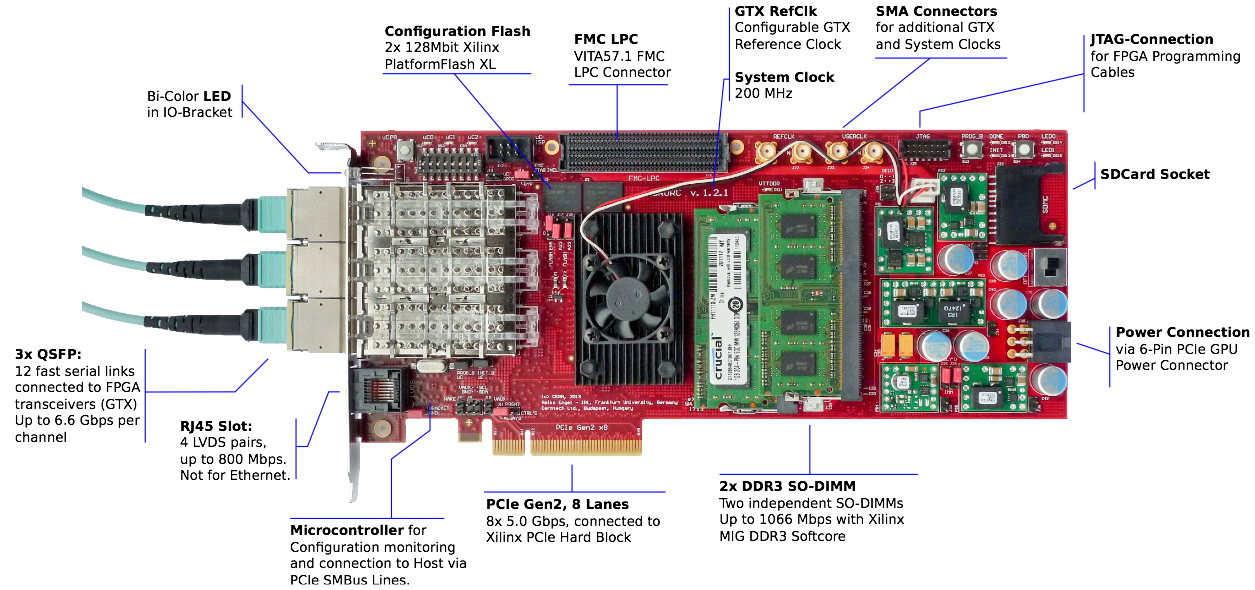
\includegraphics[width=\textwidth]{crorc.png}
\caption{Photo of the C-RORC board with the major components and features annotated \cite{crorc}.}
\label{fig:crorc}
\end{figure}

\begin{figure}[tbp] % figures (and tables) should go top or bottom of
                    % the page where they are first cited or in
                    % subsequent pages
\centering
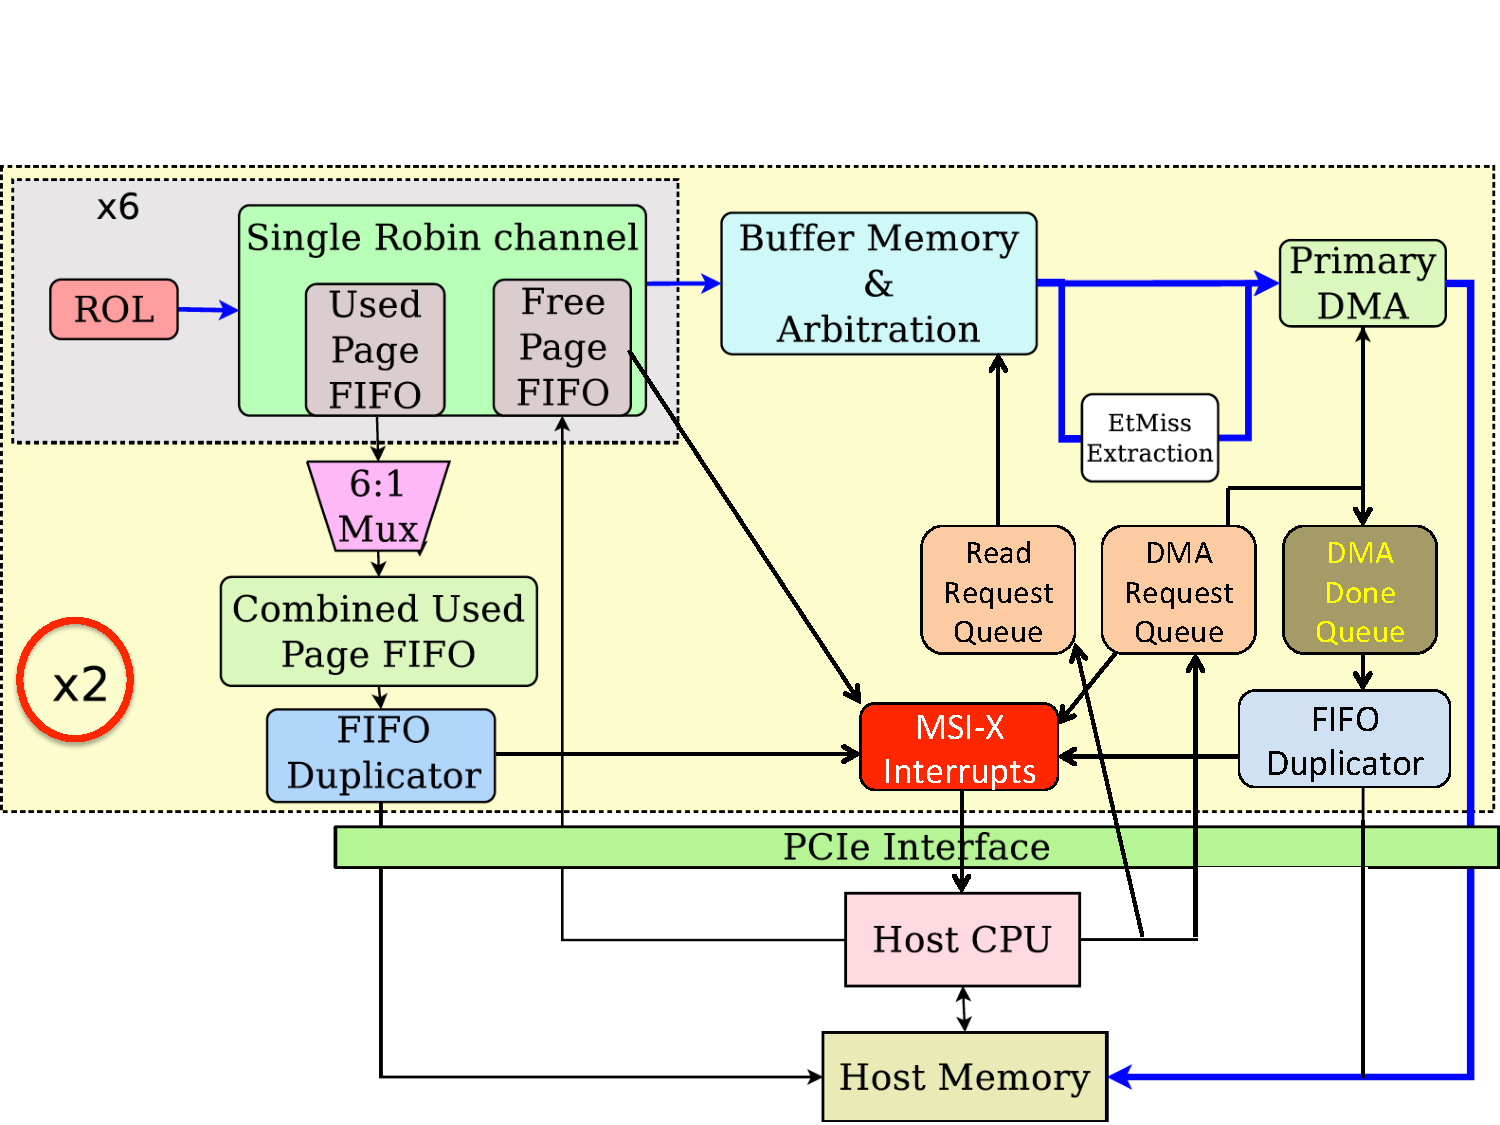
\includegraphics[trim = 0cm 0cm 0cm 2.5cm, clip, width=.71\textwidth]{RobinNP_Firmware}
%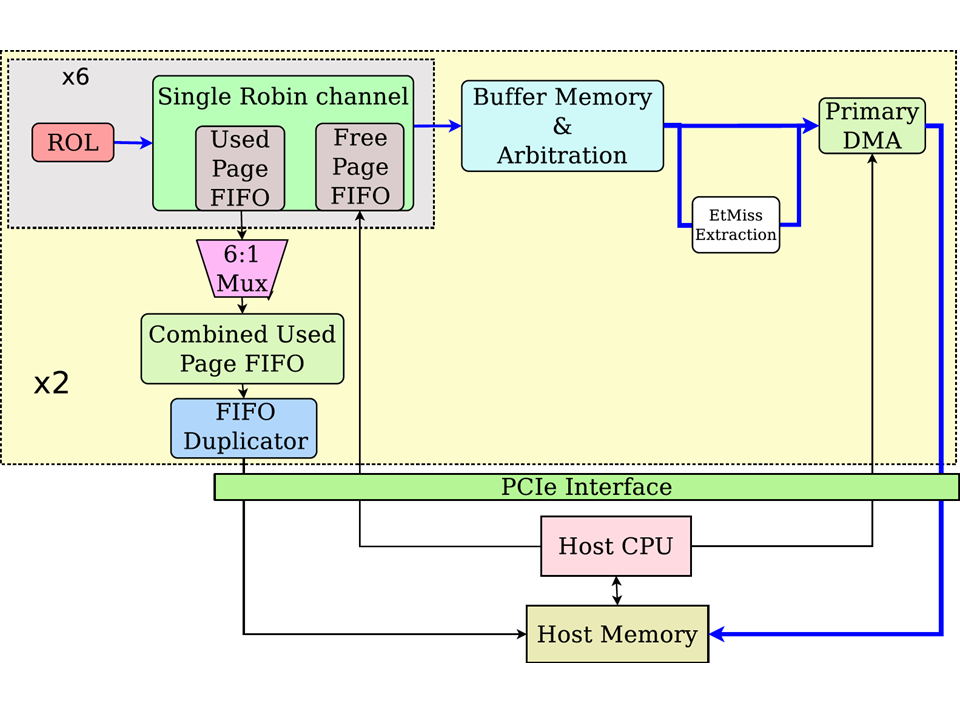
\includegraphics[width=.6\textwidth]{Firmware.jpg}
%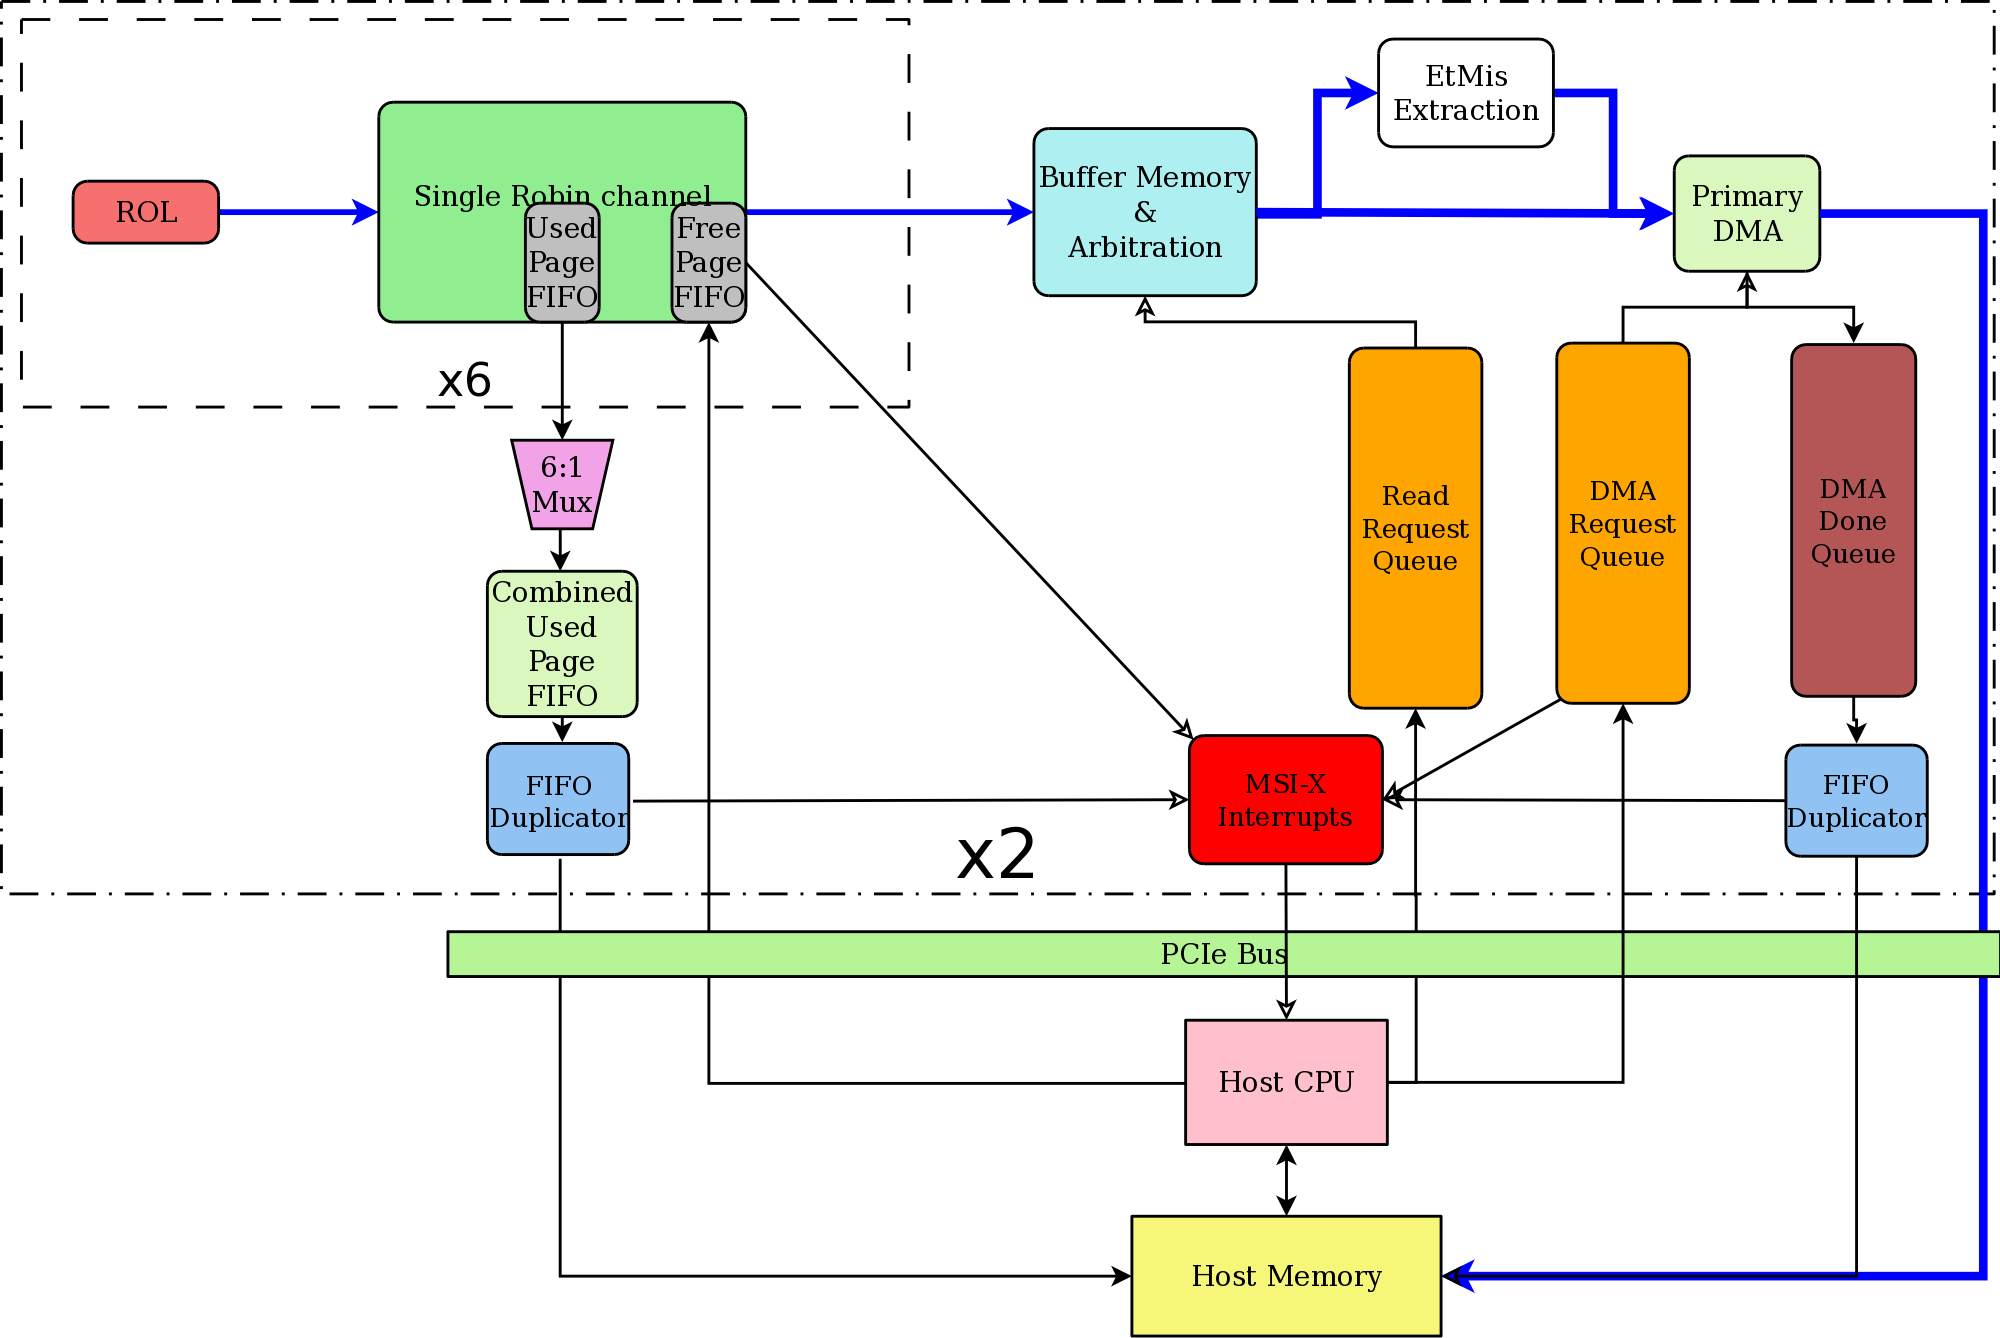
\includegraphics[width=.8\textwidth]{AReducedBlockDiagram.png}

\caption{RobinNP firmware organization
and  flow  of  data  from  host  CPU  to  the
firmware  (by  means  of  programmed  I/O)
and from the firmware to the host memory
(by means of DMA).}
\label{fig:robinnp_fw}
\end{figure}

\subsection{Readout System Firmware \& Software}\label{sec:crorc_fw}

The RobinNP firmware used for the RoIB is identical to that used in the ATLAS ROS\cite{ros}. As shown in 
the schematic of Figure \ref{fig:robinnp_fw}, the logic is divided into two functional blocks, known as sub-ROBs, 
each servicing six input links and one DDR3 memory module. Event data fragments arriving via a link are subjected 
to a range of error checks before being stored in the memory module for the relevant sub-ROB. At the same time a token
representing the address of a region of the memory, referred to as a page, is passed to a listening software process via 
a `FIFO duplicator'. To avoid a costly read across the PCIe bus, data is continuously streamed from firmware to 
software via a chain of firmware and software FIFOs. Notification of new data arriving in the software FIFO is managed via coalesced 
interrupts to allow for efficient use of CPU resources.
For the RoIB application, the receipt of page information immediately triggers a DMA of fragment data from the RobinNP memory into 
the host PC memory. The fragments are then passed via a queue (one per sub-ROB) to the RoIB process along with any relevant fragment 
error information. A schematic of this shortened dataflow path is presented in Figure \ref{fig:roib_swfw}. 
The API for the RoIB process consists of these queues, return queues for processed pages now available for re-use and 
a configuration interface. The software is implemented with multiple threads each handling specific tasks such as supply of free pages, receipt
of used pages, DMA control and bulk receipt of fragment data.


\begin{figure}[tbp] % figures (and tables) should go top or bottom of
                    % the page where they are first cited or in
                    % subsequent pages
\centering
%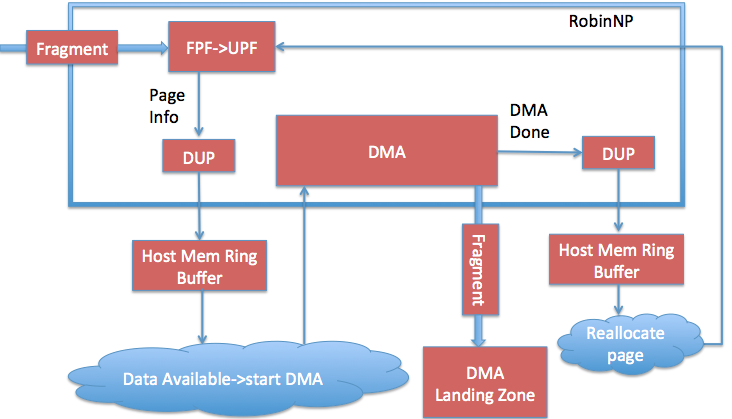
\includegraphics[width=.6\textwidth]{roib_firmware.png}
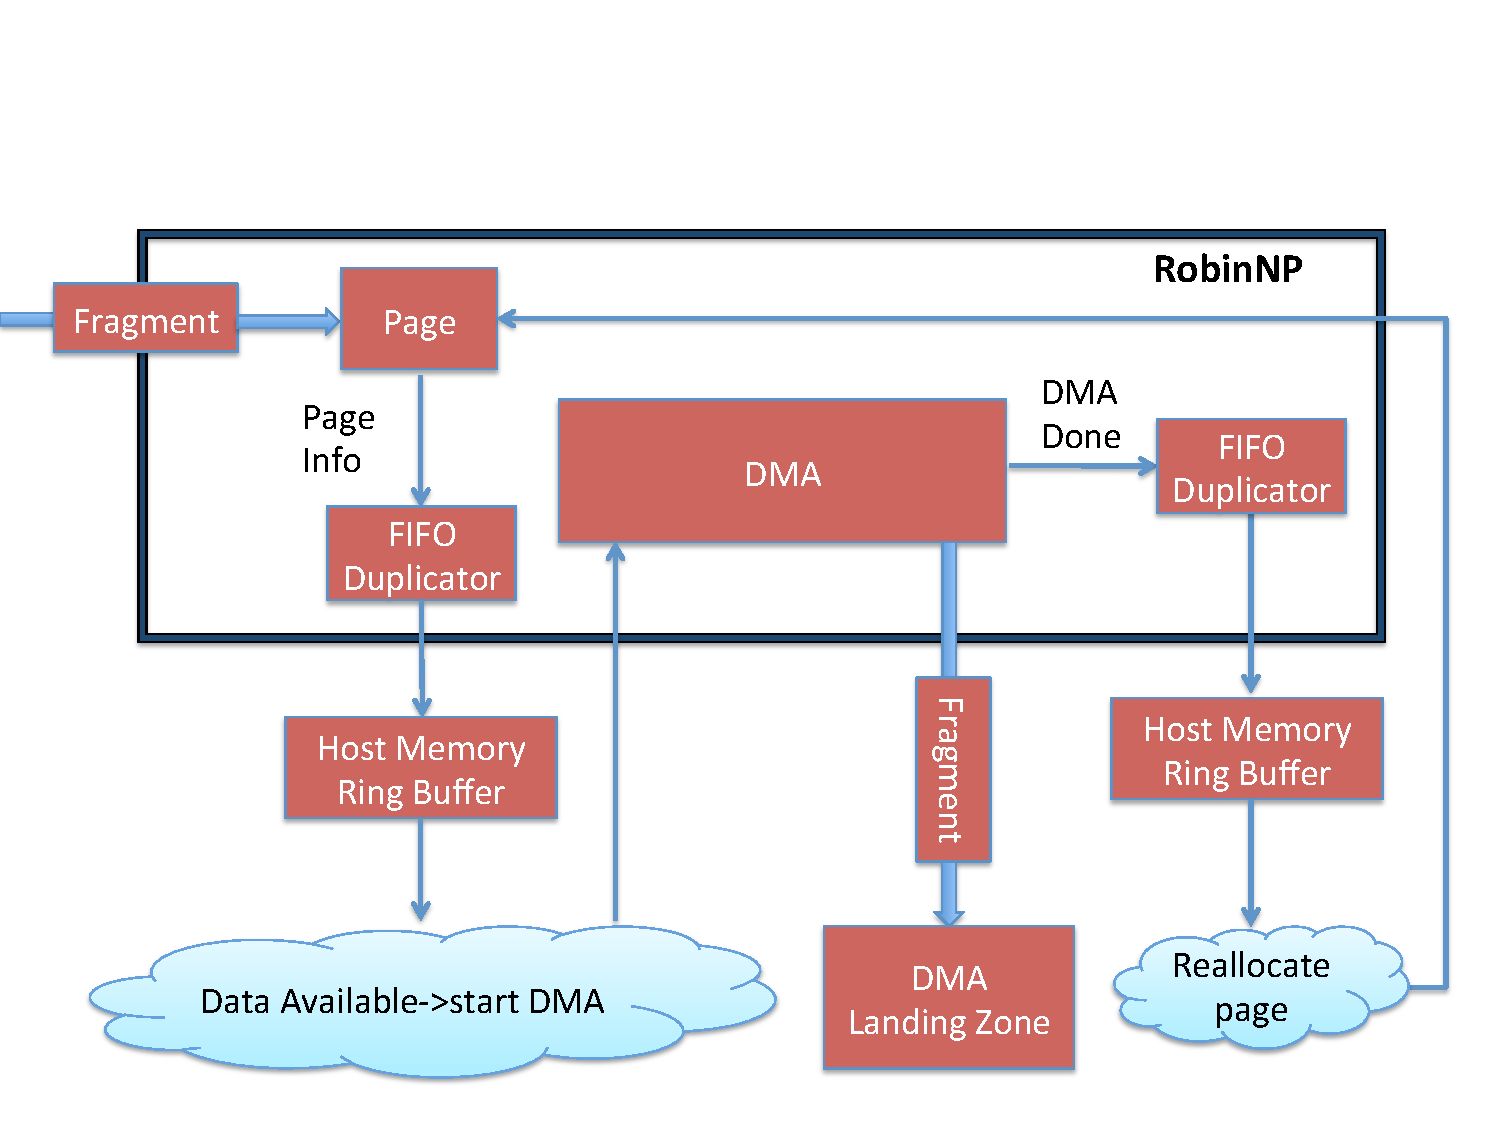
\includegraphics[trim = 0cm 0cm 0cm 5cm, width=.7\textwidth]{RobinNP_Software}
\caption{Layout of the readout system firmware and software specific to the RoIB.}
\label{fig:roib_swfw}
\end{figure}

\subsection{RoIB Software}\label{sec:crorc_sw}

The HLTSV is a multi-threaded application that obtains a L1 result from a variety of possible input sources and exchanges information with the 
rest of the HLT computing farm. 
%Data Collection Managers (DCM). The DCM is the application running on each HLT computing node that tells the HLTSV if the event has been rejected, successfully built, or timed out and also requests the data from the ROS. In this case, 
For the RoIB, the L1 source is a RobinNP interface that performs fragment assembly and is used as a plug-in to the HLTSV application.
The RobinNP plug-in has two receive threads, each 
thread services six channels by pulling fragments from the RobinNP on-board memories to the host PC.
Fragments with the same L1ID are copied 
to a contiguous memory space and a queue of completed events is prepared. 
Upon request by the HLTSV, a pointer to the contiguous memory space is passed back to the 
HLTSV process for further handling. In order to optimize concurrent access to RoIB data structures, containers from the  Intel 
threading building block (TBB) library were used. These containers allow multiple threads to concurrently access and update items 
in the container while maintaining high performance.  


\section{Prototype Tests}\label{sec:perf}

In order to understand the requirements for the underlying server PC, a validation system based on Intel(R) Xeon(R) CPU E5-1650 v2 
@ 3.5 GHz with six cores is being used to perform tests of the PC based RoIB. 
The goal is to perform software based fragment assembly at a rate of 100 kHz over 12 channels for a typical 
fragment size of 400 bytes. The current system offers flexibility in terms of the fragment size allowed which was not the case in the 
VMEbus based RoIB. The initial tests were performed with a standalone application that implements a minimal interface for event building. 
Once the system was validated, the relevant code modules were integrated into an HLTSV process running within the full ATLAS TDAQ 
software suite with appropriately scaled test hardware to represent the remaining elements of the system.

\subsection{Standalone Tests}\label{sec:perf_alone}

The goal was to test input/output bandwidth limitations of the RobinNP and the rate of event building. Initial performance testing used 
a standalone RobinNP application and an external source that emulates the L1 trigger data 
in the form of 32-bit word fragments with 12 channels. In this test, the host PC was running the assembly routine with a single threaded application.  Figure \ref{fig:cern_robinnproib} shows the input rate without 
event building as a function of fragment size. For 400 byte fragments the input rate to the RobinNP is 215 kHz. 
The same figure 
shows the event building rate which is 150 kHz. This performance shows that the event building 
at the required rate of 100 kHz with 12 channels is achievable in a standalone application.  


\begin{figure}[tbp] % figures (and tables) should go top or bottom of
                    % the page where they are first cited or in
                    % subsequent pages
\centering
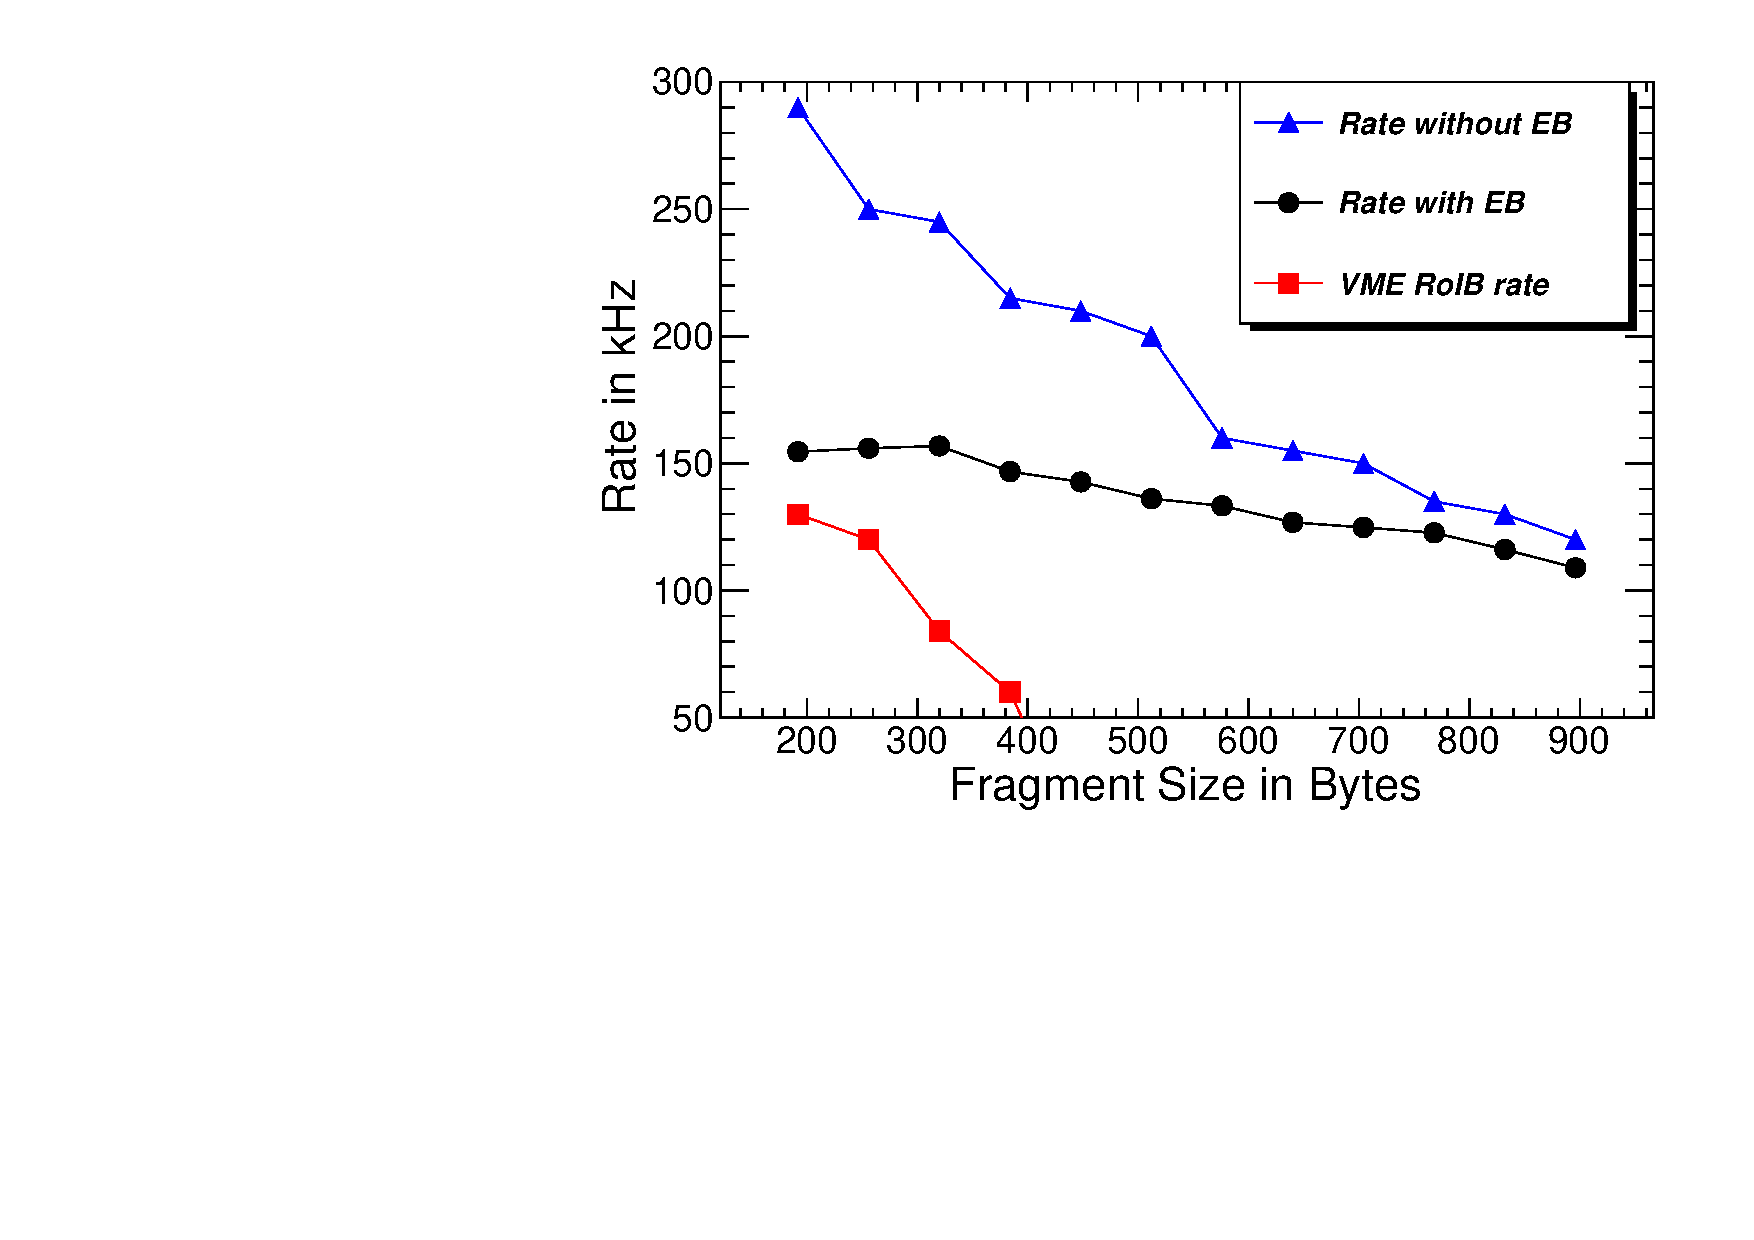
\includegraphics[width=.7\textwidth]{cern_robinnproib.pdf}
\caption{Rate as a function of the fragment size (in bytes) with external source that emulates the L1 trigger input. 
The rates shown are for the input rate to the RobinNP without event building (EB) (triangle), rate with EB (circle), and 
for comparison, the current VMEbus RoIB rate is also shown (square).  }
\label{fig:cern_robinnproib}
\end{figure}


\subsection{Full System Tests}\label{sec:perf_tdaq}

Since the HLTSV is performing tasks other than the event building, there is overhead associated with additional operations 
that reduces the performance. For this reason, we use the full ATLAS TDAQ software in a test environment that emulates the major components of the ATLAS data acquisition system shown in Figure \ref{fig:atlas_tdaq}. The setup includes an emulated input from L1 trigger sources, 
the HLTSV and other PCs to simulate the HLT computing farm, and the ROS that buffers the full event data. 
 In this test setup, an external source sends data that emulates L1 RoIs via 12 links connected to the 
RobinNP hosted by the HLTSV. When the HLTSV requests a built RoI event, the software RoIB plug-in provides the RoI event which will be used 
to seed requests for the event data to be processed.
 Figure \ref{fig:partition} shows an event building rate of 110 kHz measured with 400 byte fragments with the HLTSV application in a setup close to the ATLAS TDAQ system. 

\begin{figure}[tbp] % figures (and tables) should go top or bottom of
                    % the page where they are first cited or in
                    % subsequent pages
\centering
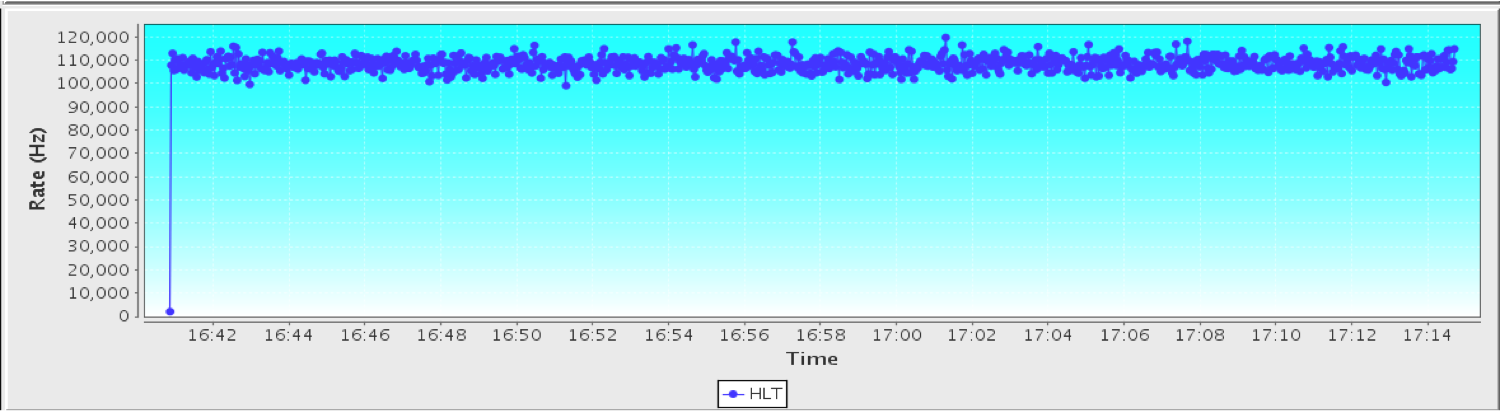
\includegraphics[width=.98\textwidth]{12ch.png}
\caption{Screenshot of a monitoring tool which shows the HLTSV processing rate using the ATLAS TDAQ software .}
\label{fig:partition}
\end{figure}


\section{Outlook}\label{sec:outlook}

The RoIB will evolve from the VMEbus based system to the PC based system using a PCI-Express card and firmware shared with the 
ATLAS ROS. The new system will add flexibility and improve maintainability of the ATLAS TDAQ system. As the technology 
evolves, the PCs and CPUs can be upgraded and more channels can be included by adding more RobinNP cards while maintaining high 
readout rates. A full integration test of the readout performance of the ATLAS TDAQ system with the PC based RoIB will be performed 
during the 2015-2016 LHC winter shutdown in preparation for a system evolution.



%% \bibitem{atlas}
%% ATLAS Collaboration, \emph{The ATLAS experiment at the CERN Large Hadron Collider}, \jinst{3}{2008}{S08003}.

%% \bibitem{evolution}
%%  N. Garelli (on behalf of the ATLAS Collaboration),
%% \emph{The Evolution of the Trigger and Data
%% Acquisition System in the ATLAS Experiment},
%% {J. Phys.: Conf. Ser.
%% 513 (2014) 012007.}



%% \bibitem{l1}
%% ATLAS Collaboration, \emph{ATLAS Level-1 Trigger: Technical Design Report}, 
%% {ATLAS-TDR-12}, 1998


%% \bibitem{hlt}
%% ATLAS Collaboration,
%% \emph{ATLAS, High-Level Trigger, Data Acquisition and Controls} \href{https://cds.cern.ch/record/616089}{https://cds.cern.ch/record/616089}
%% \emph{CERN/LHCC/2003-022}, CERN Geneva 2003.






%% \bibitem{ros}
%% A. Borga et al.,\emph{Evolution of the ReadOut System of the ATLAS experiment}, in proceedings of
%% \emph{Technology and Instrumentation in Particle Physics 2014}, June, 2--6, 2014 Amsterdam, the Netherlands
%% \pos{PoS(TIPP2014)205}.



%% \bibitem{vme_roib}
%% R. Blair et al.,
%% \emph{The ATLAS High Level Trigger Region of Interest Builder},
%% \jinst{3}{2008}{P04001} 


%% \bibitem{swroib_past}
%% R. E. Blair et al., \emph{ATLAS TDAQ dataflow: Software RoI builder status report}, {ATL-DQ-TR-0020}, 2012


%% \bibitem{l1ttc}
%% S. Ask et al., \emph{The ATLAS central level-1 trigger logic and TTC system}, \jinst{3}{2008}{P08002}.

%% \bibitem{tilar}
%% CERN, \url{http://www.cerntech.hu/products/15-tilar-express.html}, October 15, 2015


%% \bibitem{alice}
%% H. Engel,U. Kebschull (For the ALICE Collaboration),
%% \emph{Common read-out receiver card for ALICE Run2},
%% \jinst{8}{2013}{C12016}.

%% \bibitem{crorc}
%% A. Borga et al., \emph{The C-RORC PCIe Card and its Application in the ALICE and ATLAS Experiments}, \jinst{10}{2015}{C02022}.





%-------------------------------------------------------------------------------
\chapter{Object Reconstruction}\label{sec:reco}
%-------------------------------------------------------------------------------
\input{texfiles/chap.reco.tex}

%-------------------------------------------------------------------------------
\chapter{Data-driven techniques to estimate fake lepton backgrounds}\label{sec:fake}
%-------------------------------------------------------------------------------
\section{The problem of fakes}

The reconstructed objects (leptons, photons, $b$jets, etc.) in a collision event are used to perform a wide range of SM measurements 
or searches for evidence of BSM physics. The assumption is that these objects are `real` representing the desired particles 
in the final state used in the analysis. 
In practice, the reconstructed objects might not be always `real`. In fact, they may be something completely different that
was mistakenly reconstructed as the desired object, called `fake`. 
For the purpose of the analysis presented in this thesis, the focus is on `fake` leptons. 
To illustrate the problem, a hadronic jet may deposit more energy in the electromagnetic calorimeter than the hadronic calorimeter, 
or that it leaves a narrow deposit of energy leading the reconstruction alogorithms to mistake this jet for an electron.
From the analysis point of view, the `fake` electron will pass all the selection criteria and will be indistinguishable from 
a `real` electron. 
It is important for the analysis that requires a reconstructed electron to model the fake electron background to get a sound 
result. This example was given with electrons, but can be generalized to muons as well. 
In short, any analysis that uses leptons in the final state must account for the `fake` lepton background. 
This background can be more or less important depending on the detector, the analysis selection, and the number of leptons required. 
To estimate this background it is important to first understand what type of processes lead to fake leptons.


\section{Common processes for faking leptons}

The reconstruction of `fake` leptons can be an instrumental effect related to the inability to identify the object based on 
its measured properties by the detector. In this case, the reconstructed lepton is not a real lepton and the production process 
will be different for electrons and muons.

The reconstruction of electrons relies on the observation of well aligned particle hits in the layers of the ID that are consistent 
with an energy deposition in the EM calorimeter. Photons can mimick this signature since they deposit energy in the EM 
calorimeter that happens to be alligned with a charged track. A jet for example containing charged and neutral pions can 
lead to such scenarios. It is possible for the jet to have one charged pion leaving a track similar to that of an electron.
The decay of $\pi^0$ mesons to photons in this jet can deposit energy in the EM calorimeter leading to the required signature.
Another mechanism that can lead to fake electrons is the emission of photons via Brehmstrahlung from high energy muons. 
The muon track can be mistaken for that of an electron and the photons interact with the EM calorimeter leading to a
signature similar to that of electrons. An additional process is that of photon conversions into a $e^+e^-$.

The reconstruction of muons relies on the observation of tracks from the ID matched to tracks from the muon spectrometer.
It is possible for charged hadrons with long lifetime to traverse the calorimeter layers and leave hits in the muon spectrometer.
These hits may coincide with other hits from the ID due to the random activity in the event. As a result, a muon can get
reconstructed. Another instance may occur when pions or kaons decay in-flight to muons in the muon spectrometer
and happen to align with the primary vertex.

The leptons that are used in the physics analyses must be coming from the hard scatter, generally referred to as prompt leptons.
There is another case where the reconstructed lepton is a real lepton but is not a lepton coming from the hard interaction,
referred to as non-prompt leptons. Non-prompt leptons can be produced from heavy flavor meson decays with a low energy activity 
around the lepton which allows it to pass isolation requirements. A good example of this type of process is the 
semi-leptonic decay of top quark pair which contribute to final states with two leptons. 

For the rest of the thesis, the fake leptons will be referred to as fake/non-prompt (FNP) leptons.
There are several methods used to perform the estimation of FNP lepton backgrounds. 
A method that the author developed will be described next along with a standard method for estimating this type of backgrounds.
The benefit of having two methods for estimating the FNP lepton background is to have enough confidence in the final estimate. 
The two methods use different assumptions which naturally leads to a more robust estimation of this difficult background.
Moreover, the final estimate of the FNP lepton background is taken as a statistical combination of the estimates from the 
two methods leading to a reduction of the systematic uncertainties on the estimate.


\section{Monte Carlo Template Method}
\graphicspath{{figures/mct/}}

\subsection{Motivation}
The processes leading to FNP leptons depend on the selection applied in the analysis. For instance, a selection with same-sign leptons 
will have contributions from top quark pair production (\ttbar) or the associated production of a vector boson and jets 
($W$+jets or $Z$+jets).%, or opposite sign $W$ pair production ($W^+W^-$). 
These processes cannot give two leptons of the same electric charge unless there is a charge mis-measurement (mainly affecting electrons) 
or that a FNP lepton was produced. It is possible to generate the processes that can contribute to a FNP lepton, such as \ttbar or 
$V$+jets, with Monte Carlo event generators processed through Geant4 detector simulation of the ATLAS detector.  
This approach will yield an estimate however it might not be reliable. For instance, the detector simulation itself might not 
reproduce the true behavior of the interaction of the physics objects with the detector, particularly when looking at rare processes 
such as the production of FNP leptons. The second limitation is in the generation of enough MC events to probe the region of the 
phase space targetted by the analysis which affects the statistical uncertainties in the estimates.
The latter concern is addressed by ensuring that the simulations for the major backgrounds (\ttbar and $V$+jets) have much 
higher event count than the corresponding number of events observed in the data sample.
In fact, these backgrounds have a large number of simulated events because they are important for many analyses 
(including SM measurements and BSM searches).
The rest of the section will concentrate on addressing the former limitation. 

****


low statistics of the tri-lepton samples and the variety of sources of fake leptons.
It is difficult to rely on data-driven (including ME-based) methods that rely on inverting the isolation requirement given we deal with multi-jet final states. Inversion of the isolation requirement produces a sample with much more energetic jets than in the sample with the un-inverted isolation. 

''
picked variables that offer good separation between processed with prompt and ``fake'' leptons.
It is nice that the corrections are close to one but they do not have to be. For example, their deviations from unity depend on the decay modes of heavy flavor hadrons that are implemented in simulations.

Is the showering of the samples used to measure the correction of the fake rate and the that of the samples it is applied to the same? if not, is there a potential systematic difference that has to be taken into account?

We used Herwig for showering of all the samples that require corrections to the fake rates.


\subsection{Description of the method}

The MC template method relies on the correct modelling of FNP leptons kinematics in 
MC simulation to extrapolate background predictions from control regions to the signal regions.
The method assumes that the kinematic shapes for each source of FNP lepton is correctly modeled in the simulations, 
and the normalization for each source is extracted in a combined fit to data control regions.
The number of normalization factors depend on the number of identified origins of the FNP lepton in the signal regions
and the control regions are designed to constrain these factors in regions enriched with FNP leptons from the same origin.

To illustrate the approach, we describe the application of the method in SS/3L analysis later described in this thesis.
The processes of interest that may lead to a FNP lepton or a charge flip are $\ttbar$ and $V$+jets. 
FNP leptons are classified using an algorithm that navigates the generator particle record to determine where the FNP lepton 
is originating from. 
The lepton is classified as either an electron or a muon that is prompt from decays of on-shell $W$ and $Z$ bosons, 
non-prompt from a heavy flavor $b$ decay (HF), or fake from mis-identification of a light flavor jet or a photon (LF). 
In the case of an electron, we further classify the prompt electrons to prompt electrons with the correct charge or with a 
charge mis-measurement, commonly named charge flip.
In total, five categories referred to as MC templates are construced following the classification illustarted 
in figure~\ref{Fig:fakes_classification}.

\begin{figure}[t!]
\centering
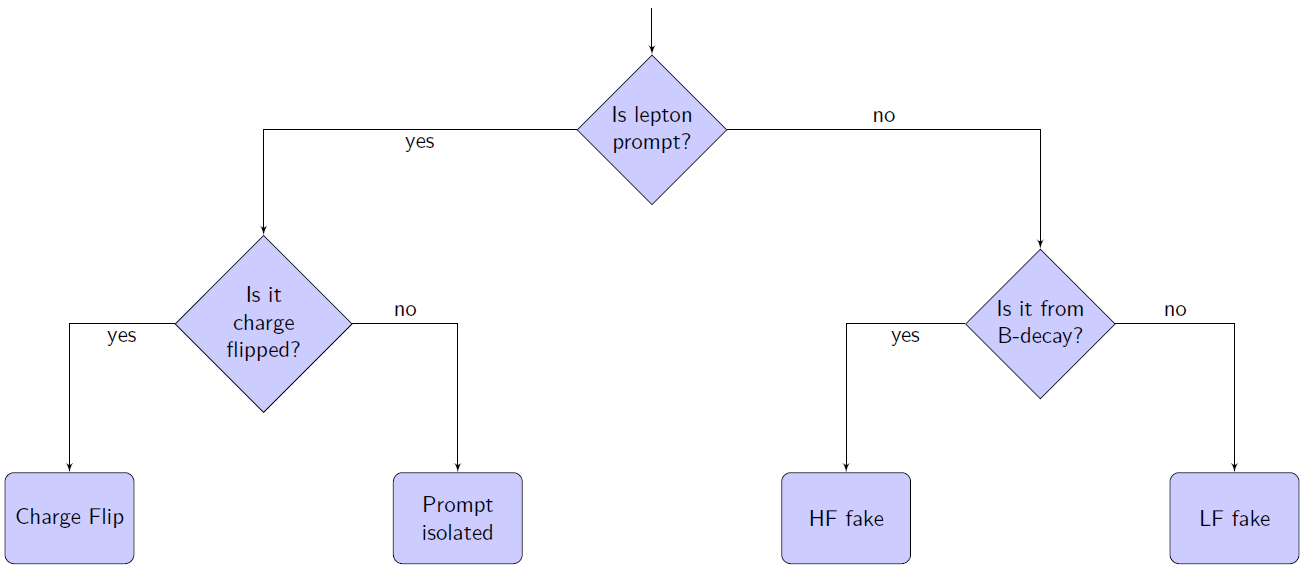
\includegraphics[width=0.7\textwidth]{MC-tmpl}
\caption
{Lepton classification.
}
\label{Fig:fakes_classification}
\end{figure}

\subsection{Correction factors}

The FNP estimate relies on kinematic extrapolation using processes expected to contribute via FNP leptons from control regions 
with low jet multiplicity and \met, to the signal regions that require high jet multiplicity and \met. 
The control regions are chosen to separate FNP leptons from HF origins and FNP leptons from LF origins.
For instance, a control sample characterized by the presence of a $b$-jet will be enriched in processes with one FNP lepton that is 
coming from a HF decay, while a sample characterized by the absence of a $b$-jet will have one FNP lepton from LF decay.
The presence of one FNP lepton in the control sample allows the correction of the production rate of these FNP leptons 
by performing a fit to data. 

For example, if a Z$\to\mu\mu$+LF jet event is reconstructed as a $\mu^+\mu^-e^+$ event, then the electron is fake.
Therefore, a correction of LF jet $\to$ e (Fr(LF$\to$e)) is applied to the rate of $\mu\mu e$ events. The correction Fr(LF$\to$e)
is constrained by a fit to data in control regions dominated by LF jet $\to$ e type fakes. 
Similarly, three other corrections are defined as LF jet $\to\mu$ (Fr(LF$\to\mu$)),  HF jet $\to$ e (Fr(HF$\to$e)),  
HF jet $\to\mu$ (Fr(HF$\to\mu$)). An additional correction is applied to correct the charge flip rate predicted by simulation.
For example, a Z$\to e^+e^-$ event is reconstructed as $e^+e^+$ or $e^-e^-$. The simulation takes into account the charge flip 
rate but it might be off. The charge flip (Cf(e)) correction derived from a data fit is expected to recover this mis-modeling.
The charge flip rate only concern electrons as the muon charge flip rate is negligeable.

A likelihood fit is defined as the product of the Poisson probabilities describing the observed events in the binned 
distributions from the expected number of events rescaled by the five multipliers which are left free to float in the fit.  
These multipliers are applied to the MC predictions in the signal regions to obtain an estimation of the charge flip and FNP backgrounds.

\subsection{Control regions}

The corrections depend on the simulated sample,
the reconstructed final state, and the flavor of the leptons. As a result, care must be taken when designing the control regions 
used to perform the fit of the FNP leptons and electron charge flip templates. 
For instance, each template needs to be constrained in a selection that is representative of the processes leading to 
FNP leptons and charge flip electrons present in the kinematic region targetted by the search for BSM physics. 

In the SS/3L analysis discussed in this thesis the control regions are defined with at least two same-sign 
leptons, $\met>40$~GeV, two or more jets. This preselection ensures that the FNP leptons are not from fakes originating from 
QCD like event topologies. 
They are further split in regions 
with or without $b$-jets to constrain the HF and LF leptons respectively. In addition, they are also split with different 
flavours of the same-sign lepton pair ee, e$\mu$, and $\mu\mu$, giving a total of six control regions. 
Any event entering the signal region is vetoed. The ee channel will constrain the charge flip correction factor, fake leptons 
 from LF decays in the selection without $b$-jets, and non-prompt decay from HF in the selection with $b$-jets. 
The $\mu\mu$ channel will constrain the muon fake rates in the LF and HF decays for the selection without or with $b$-jets, 
respectively. The e$\mu$ channel will constrain both the electron and muon fakes for events containing both lepton flavors. 

The six distributions are chosen for variables that provide the best separation between processes with prompt leptons and processes with FNP leptons and charge flip and are shown 
before and after the fit in Figures \ref{f:prefit_CR0b}-\ref{f:prefit_CR1b} and Figures \ref{f:postfit_CR0b}-\ref{f:postfit_CR1b}, respectively. 

 \begin{figure}[htb]
   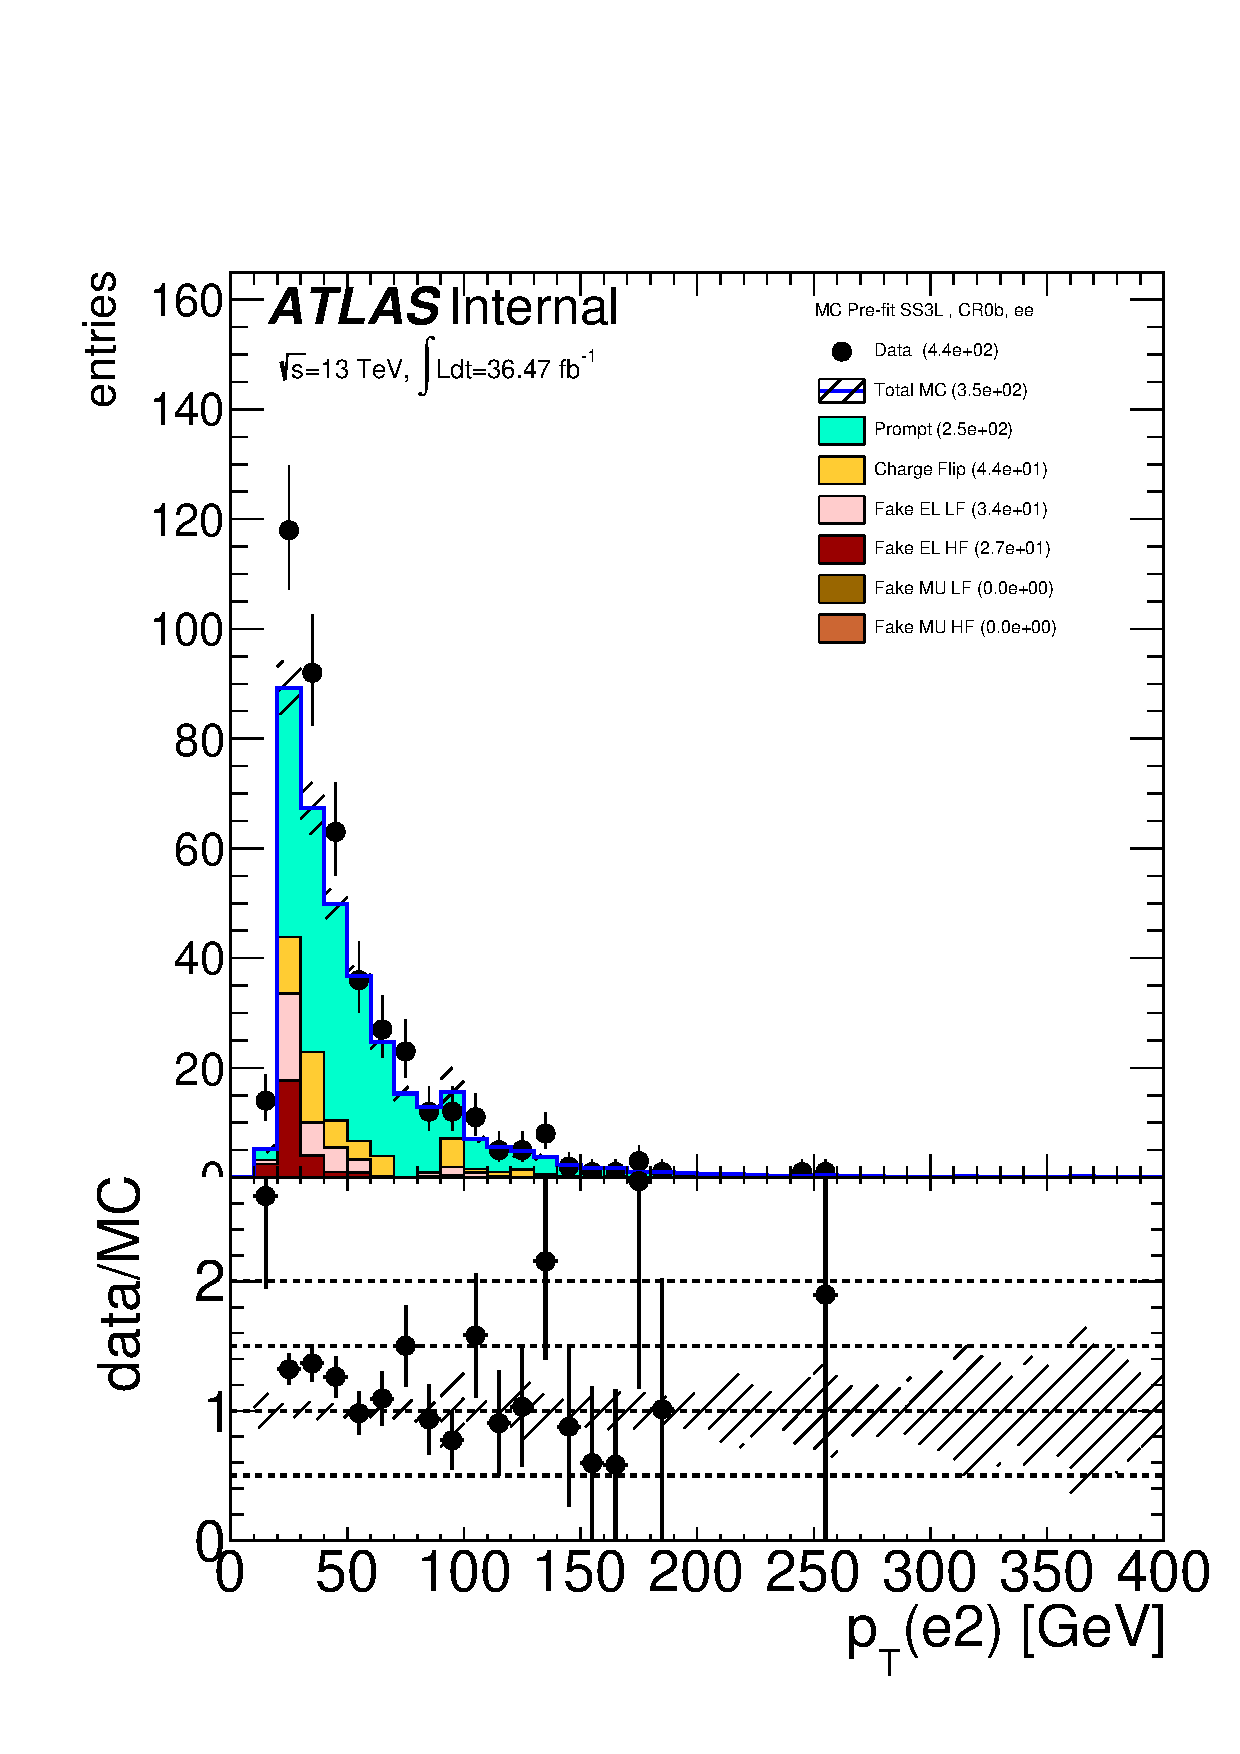
\includegraphics[width=.32\textwidth]{figures/mct/Prefit/el2_pt_ee_CR0b_SS3L}
   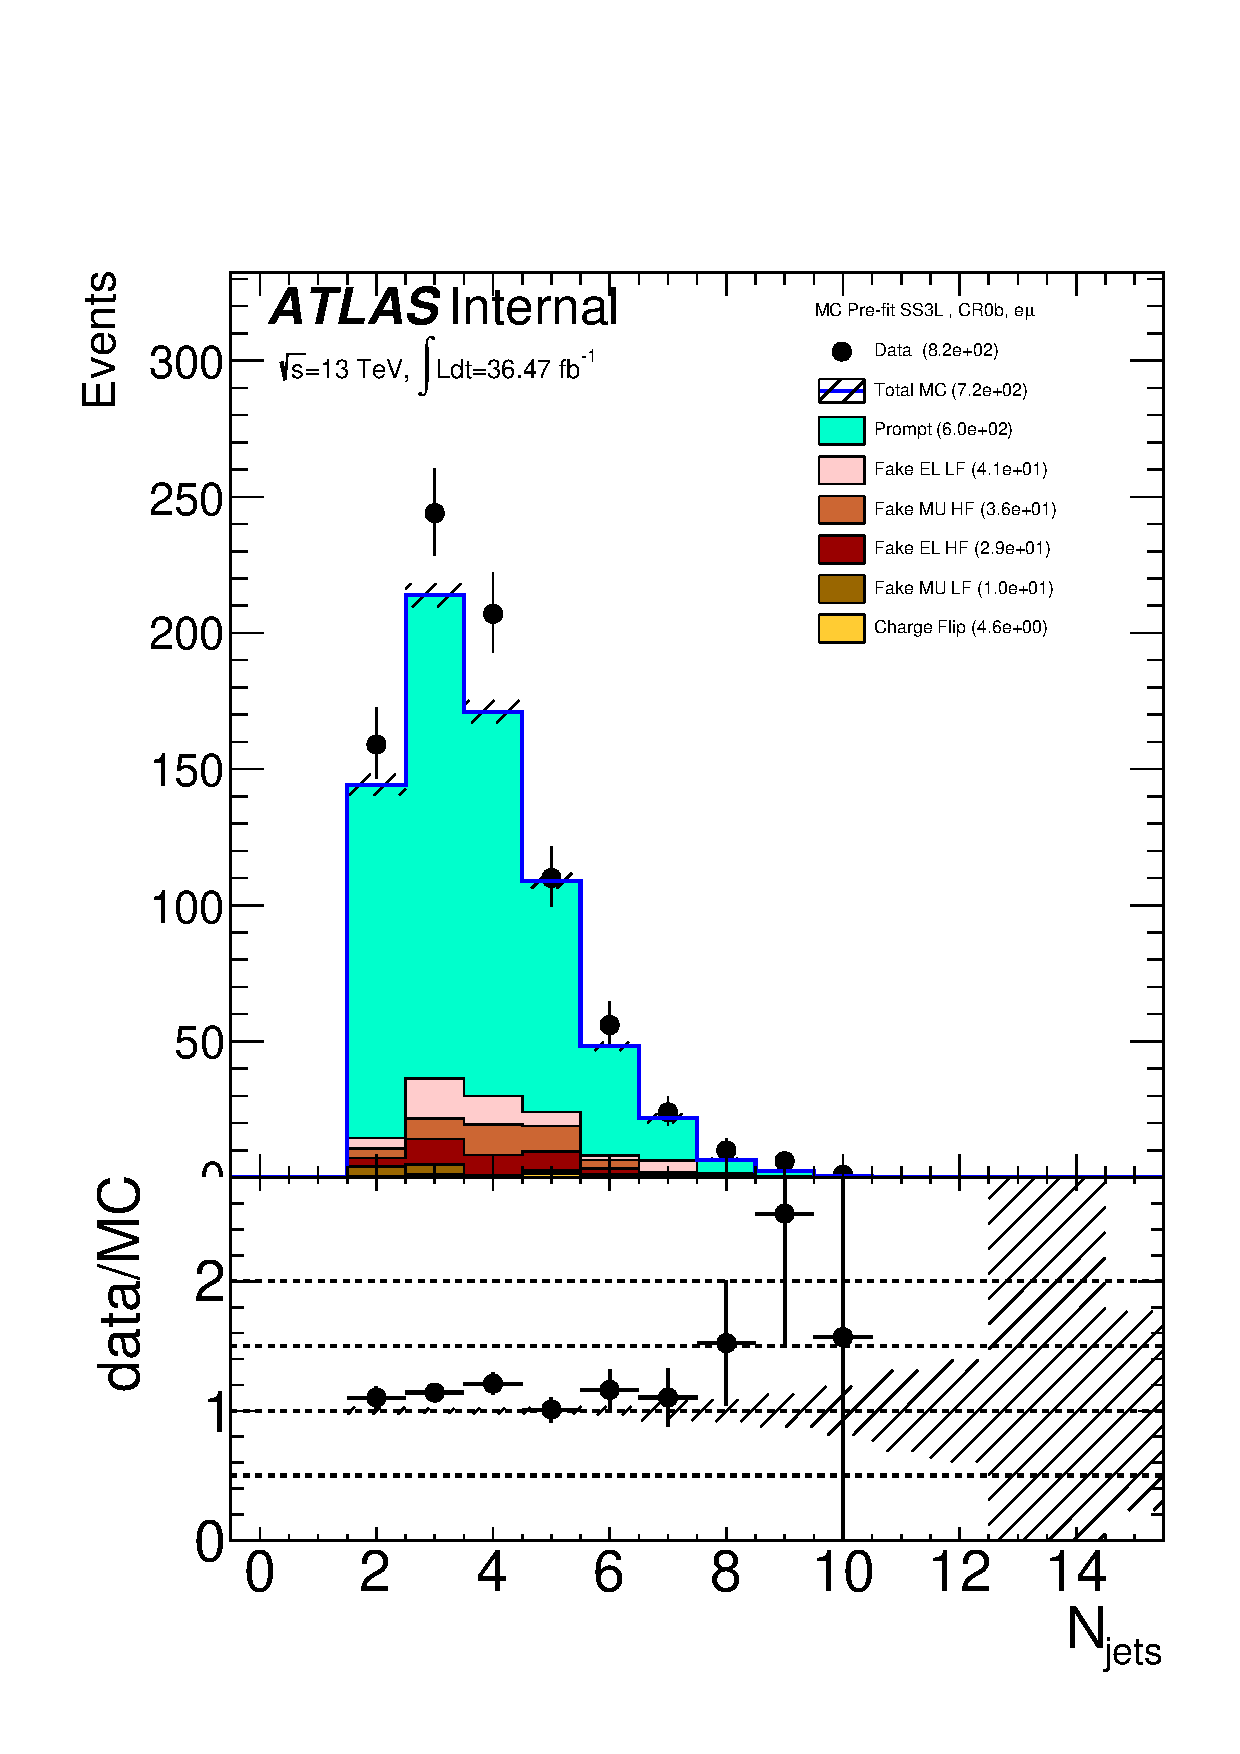
\includegraphics[width=.32\textwidth]{figures/mct/Prefit/NJETS_em_CR0b_SS3L}
   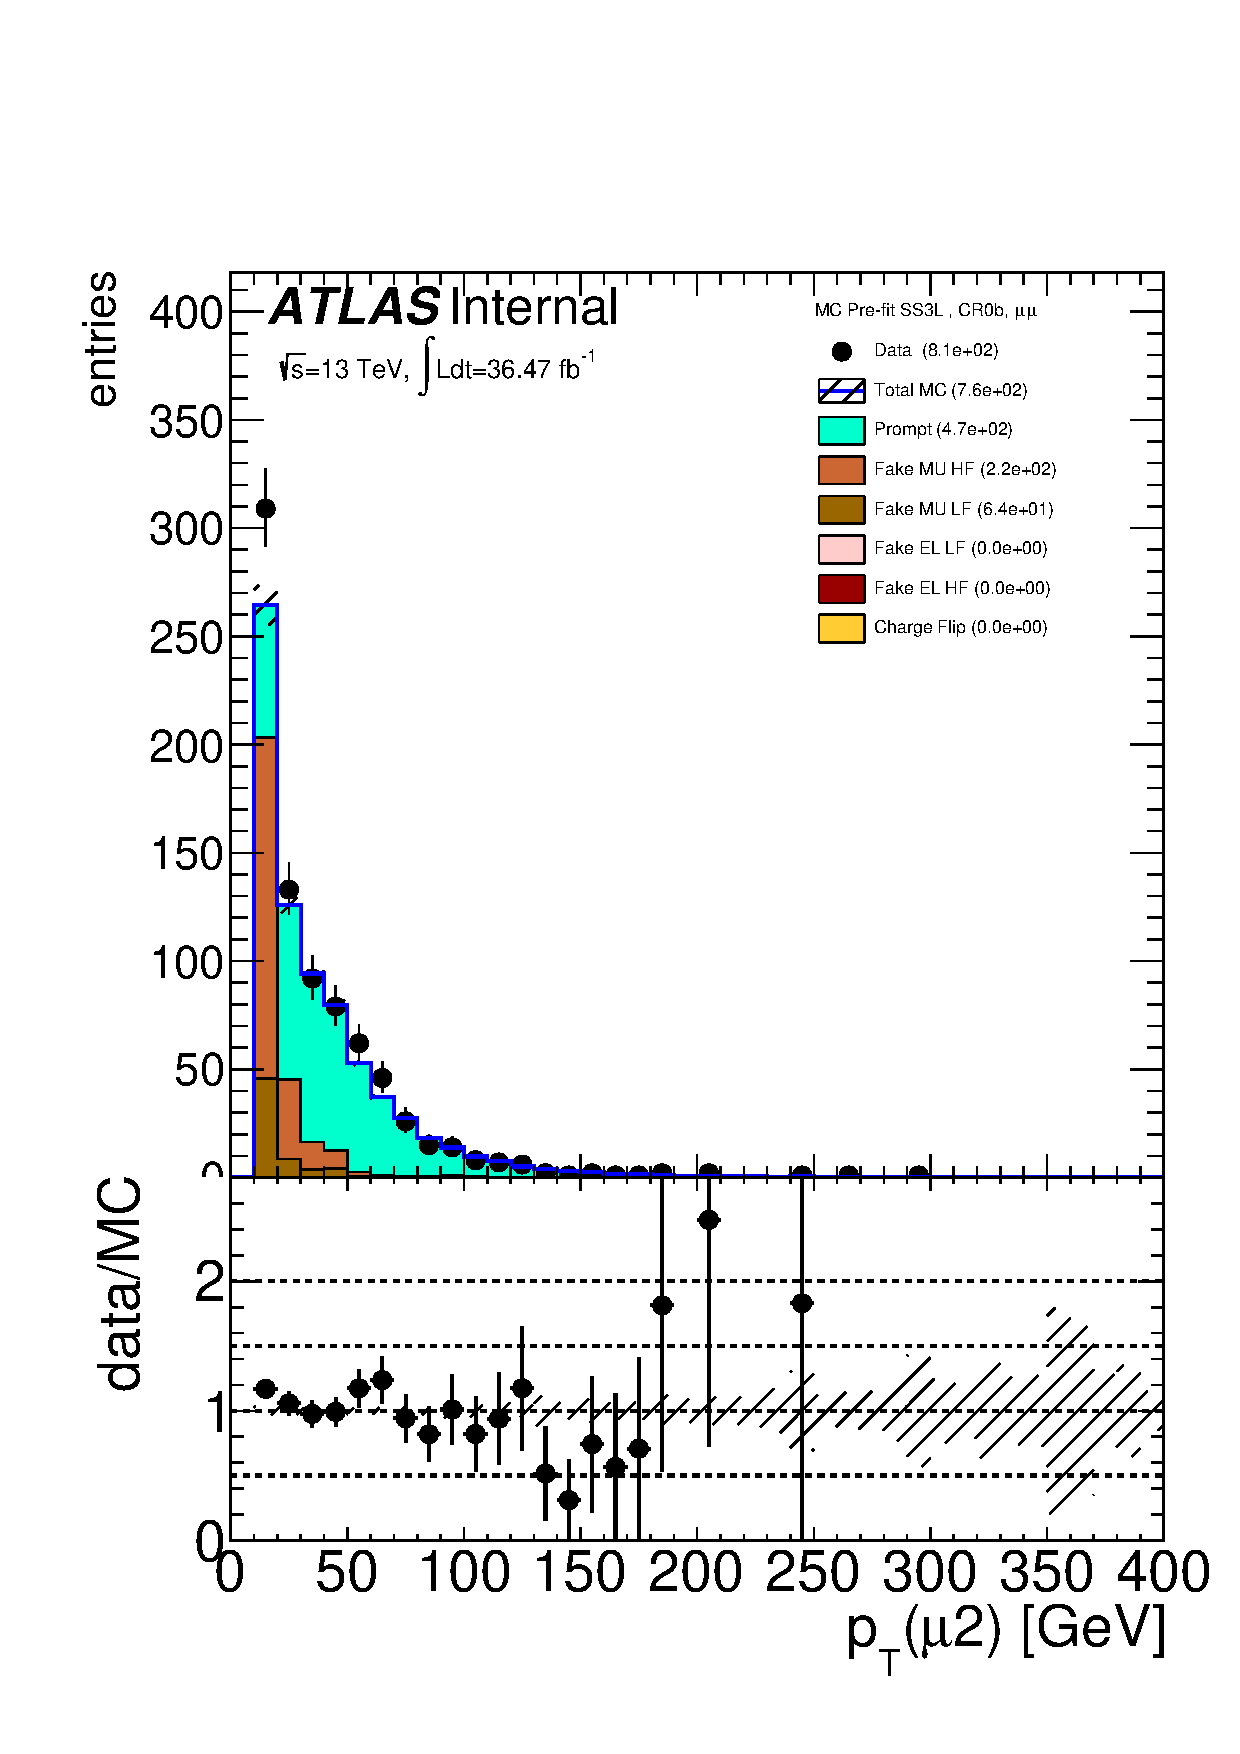
\includegraphics[width=.32\textwidth]{figures/mct/Prefit/mu2_pt_mm_CR0b_SS3L}
 \caption{
 Pre-fit distributions for  $ee$ channel (left),  for  $e\mu$ channel (middle), and  for  $\mu\mu$ channel (right) from CR0b that were used in the fit to extract the FNP lepton and charge flip multipliers.
The generator used in these plots is Powheg. The hashed band represents the sum of systematic uncertainties on the predictions.
 \label{f:prefit_CR0b}
 }
 \end{figure}

\begin{figure}[htb]
  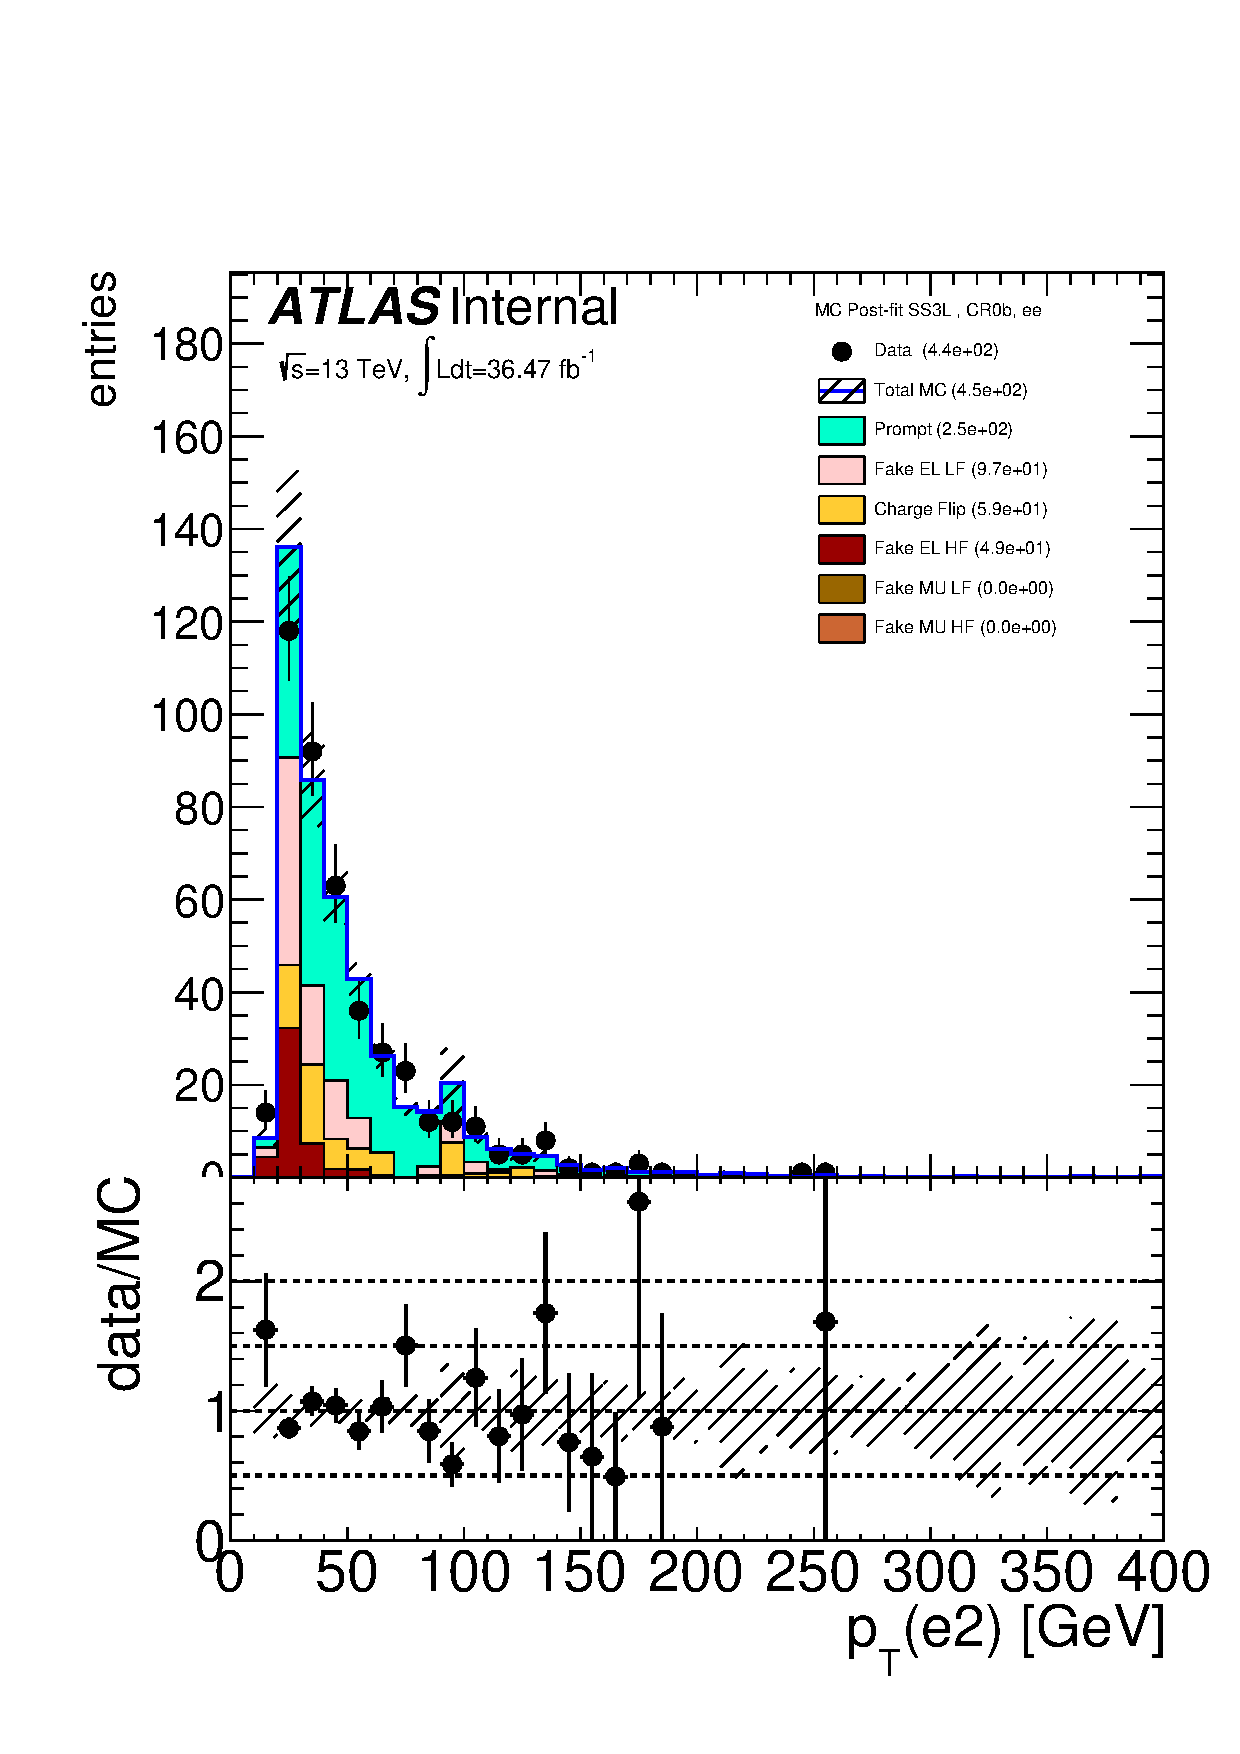
\includegraphics[width=.32\textwidth]{figures/mct/Postfit/el2_pt_ee_CR0b_SS3L}
  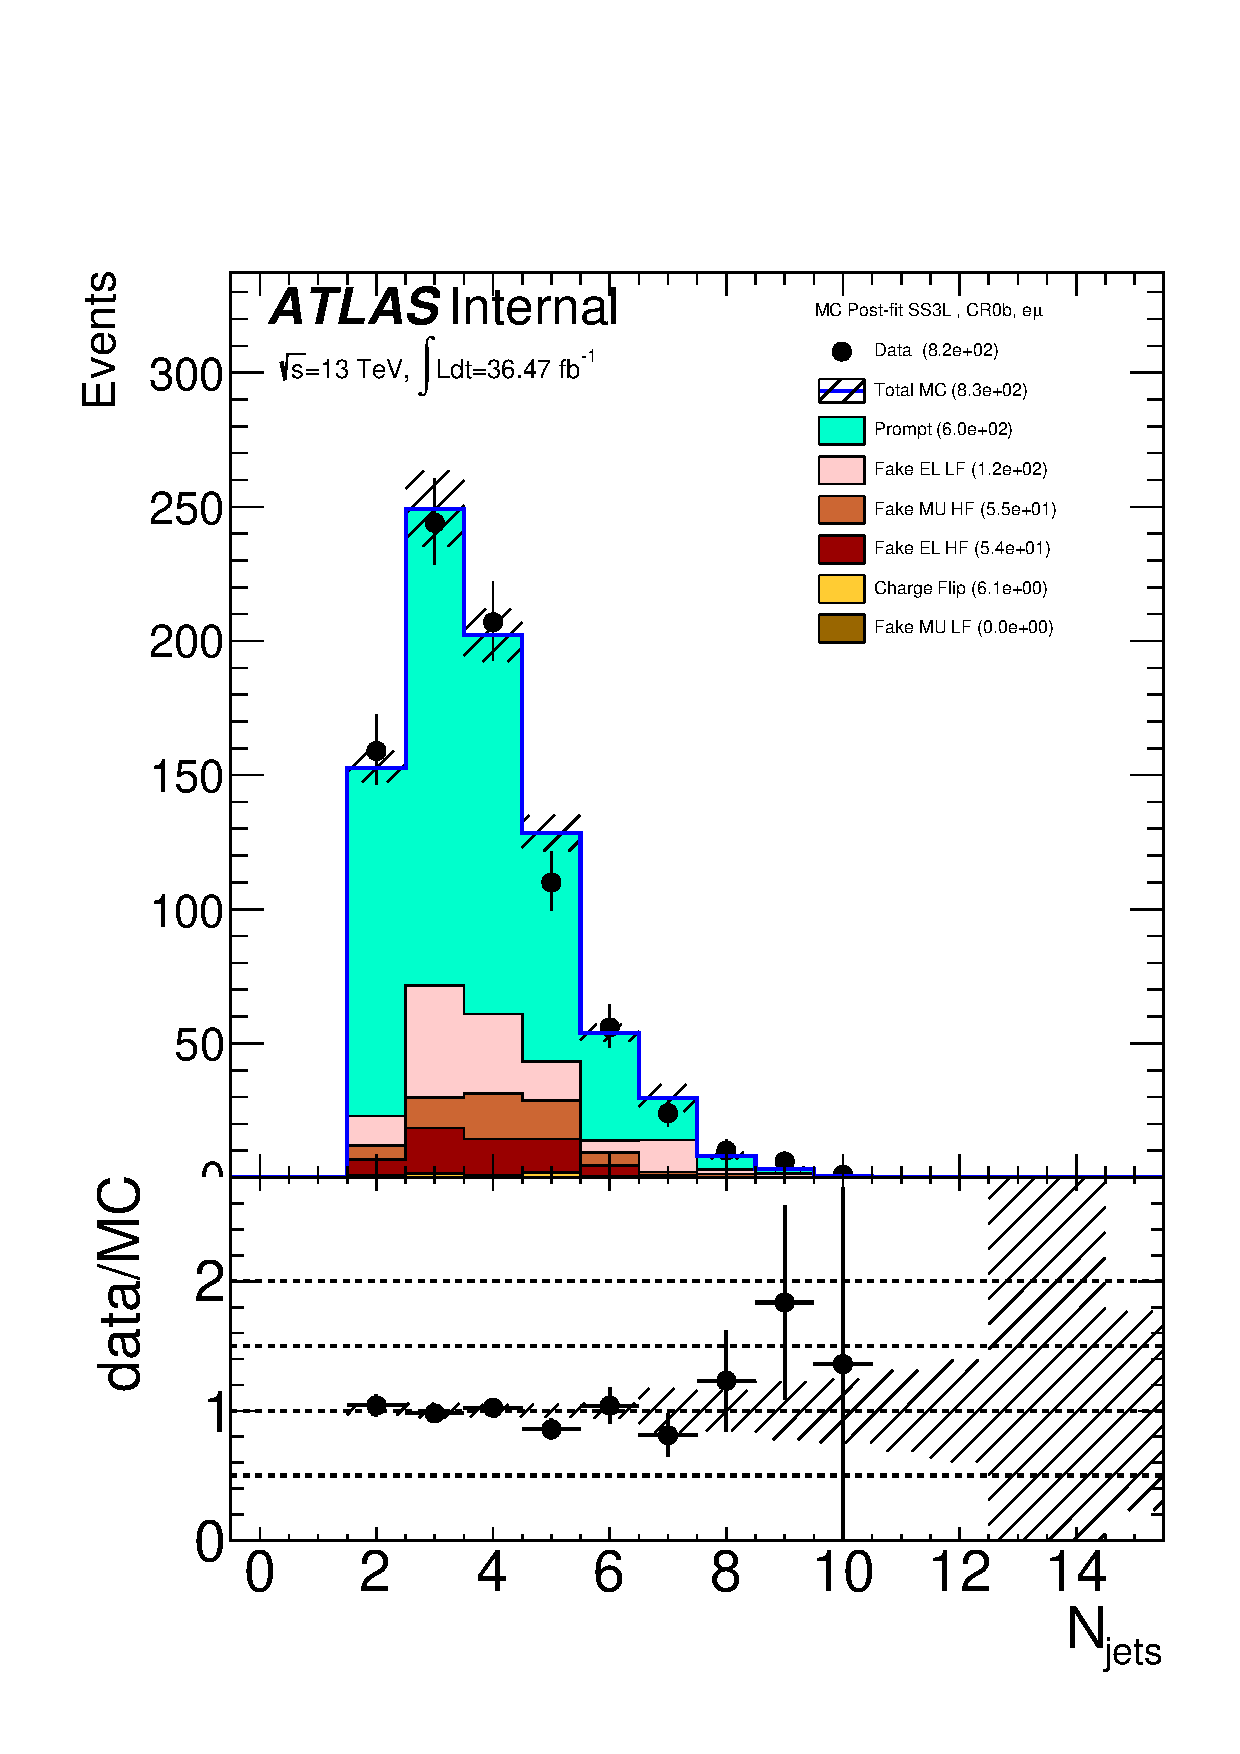
\includegraphics[width=.32\textwidth]{figures/mct/Postfit/NJETS_em_CR0b_SS3L}
  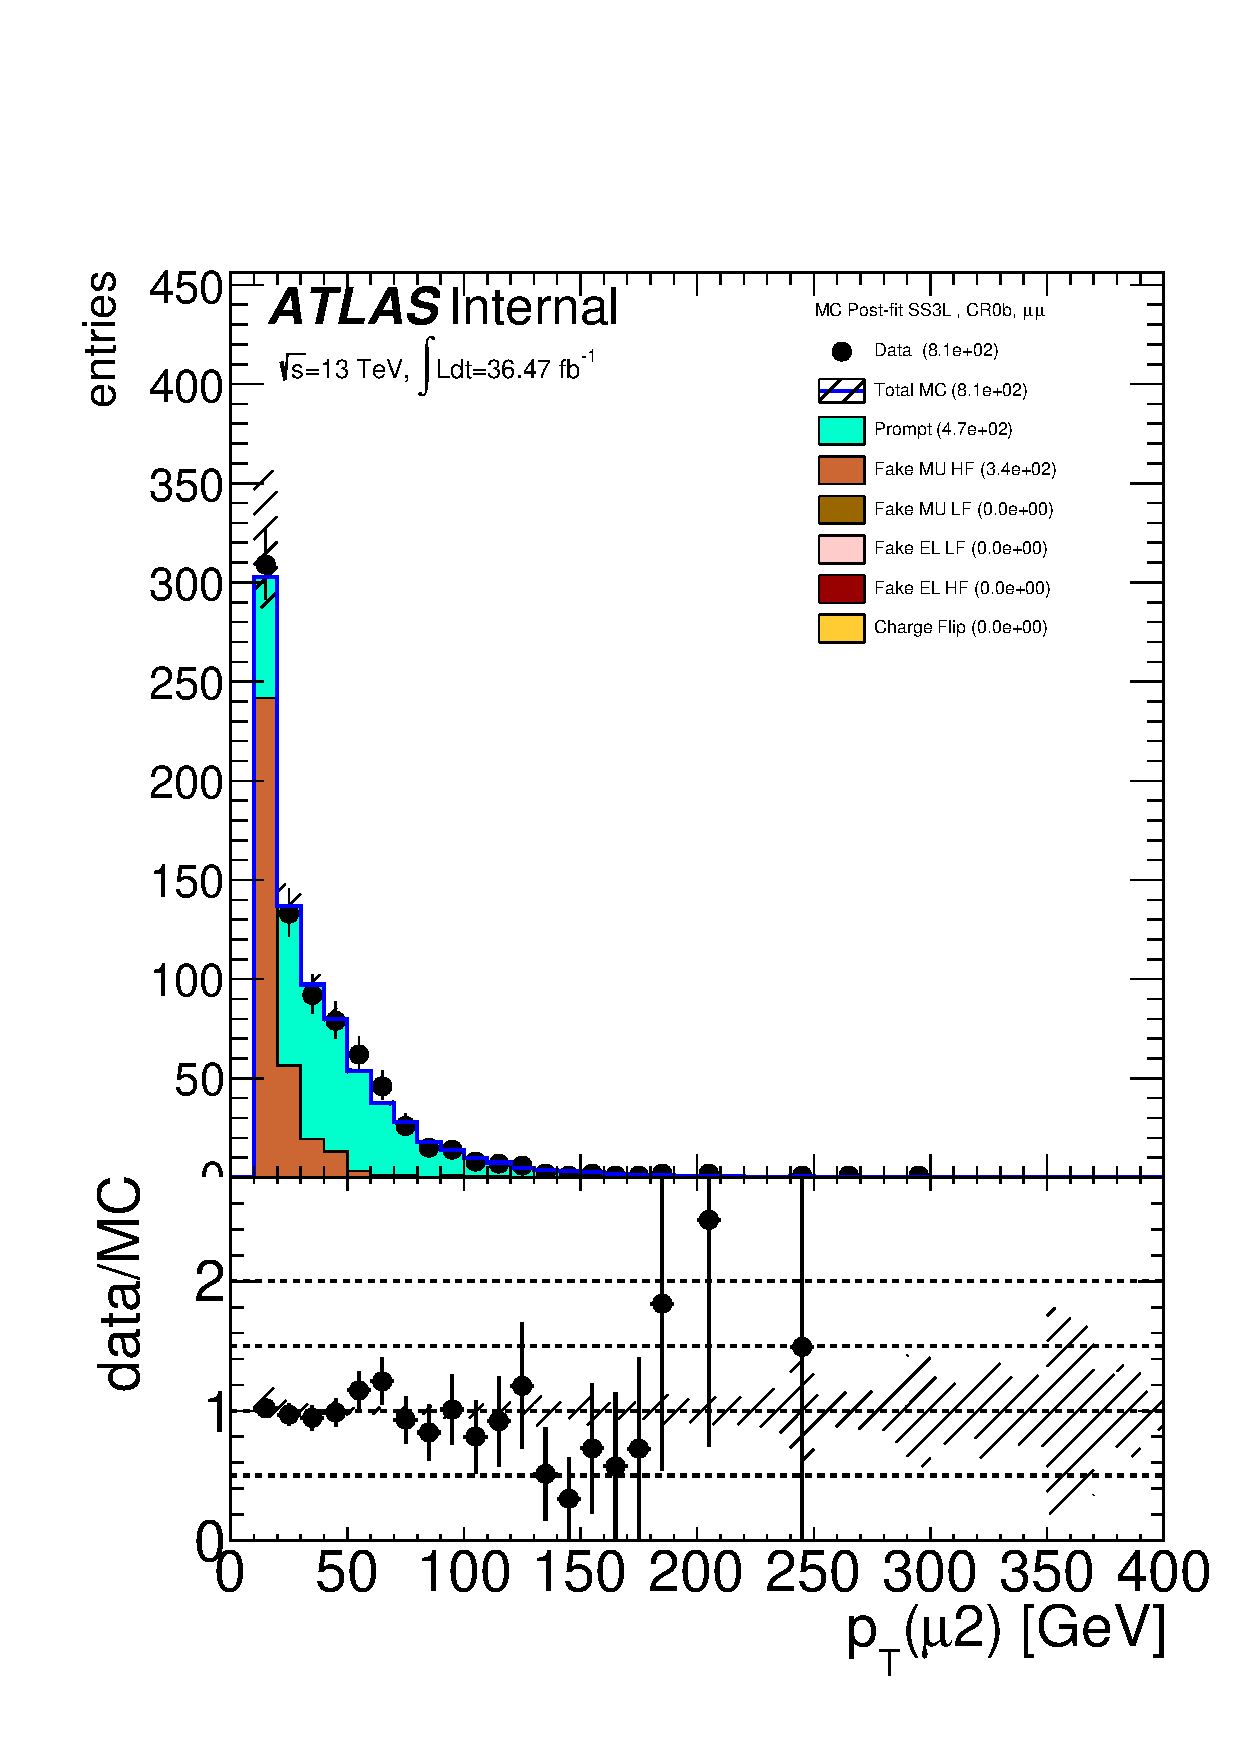
\includegraphics[width=.32\textwidth]{figures/mct/Postfit/mu2_pt_mm_CR0b_SS3L}
\caption{
Post-fit distributions for  $ee$ channel (left),  for  $e\mu$ channel (middle), and  for  $\mu\mu$ channel (right) from CR0b that were used in the fit to extract the FNP lepton and charge flip multipliers.
The generator used in these plots is Powheg. The hashed band represents the sum of systematic uncertainties on the predictions.
\label{f:postfit_CR0b}
}
\end{figure}

 \begin{figure}[htb]
   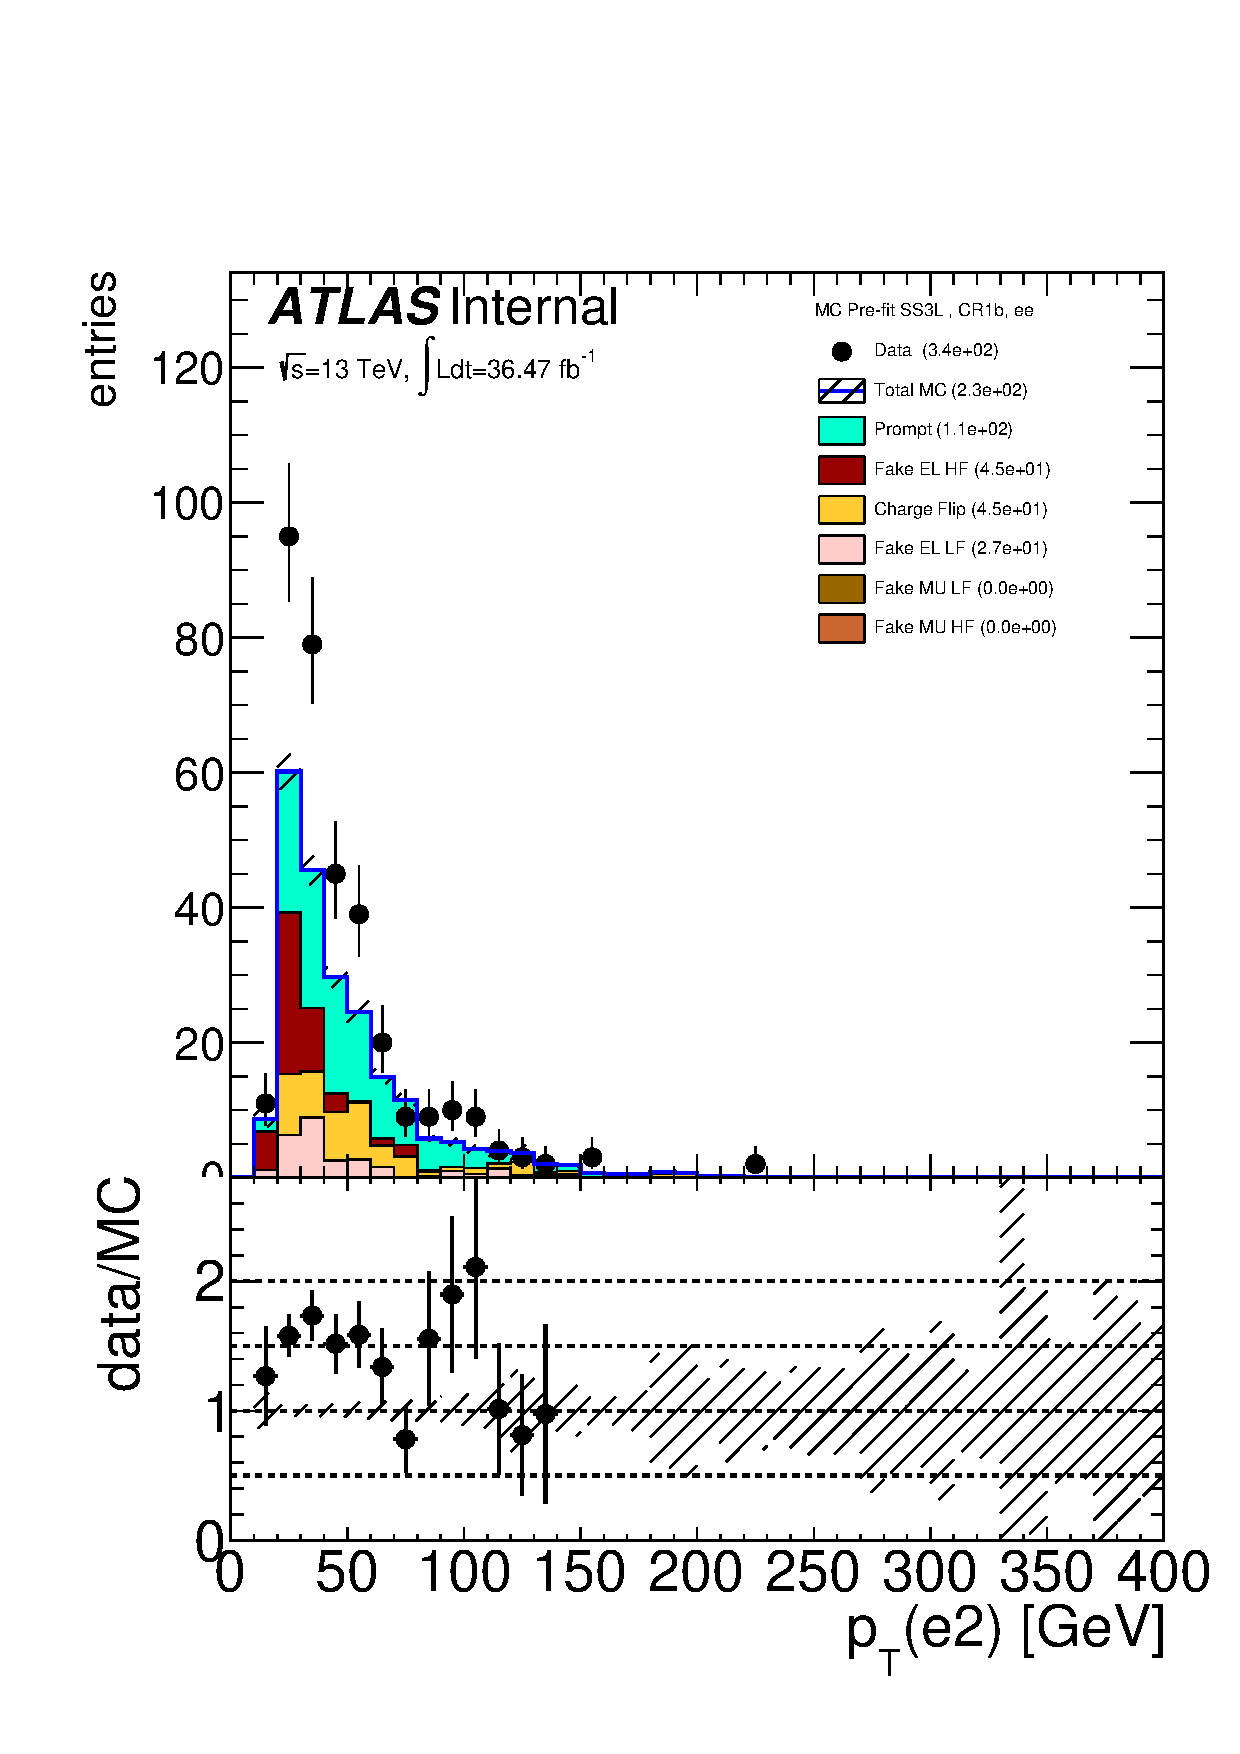
\includegraphics[width=.32\textwidth]{figures/mct/Prefit/el2_pt_ee_CR1b_SS3L}
   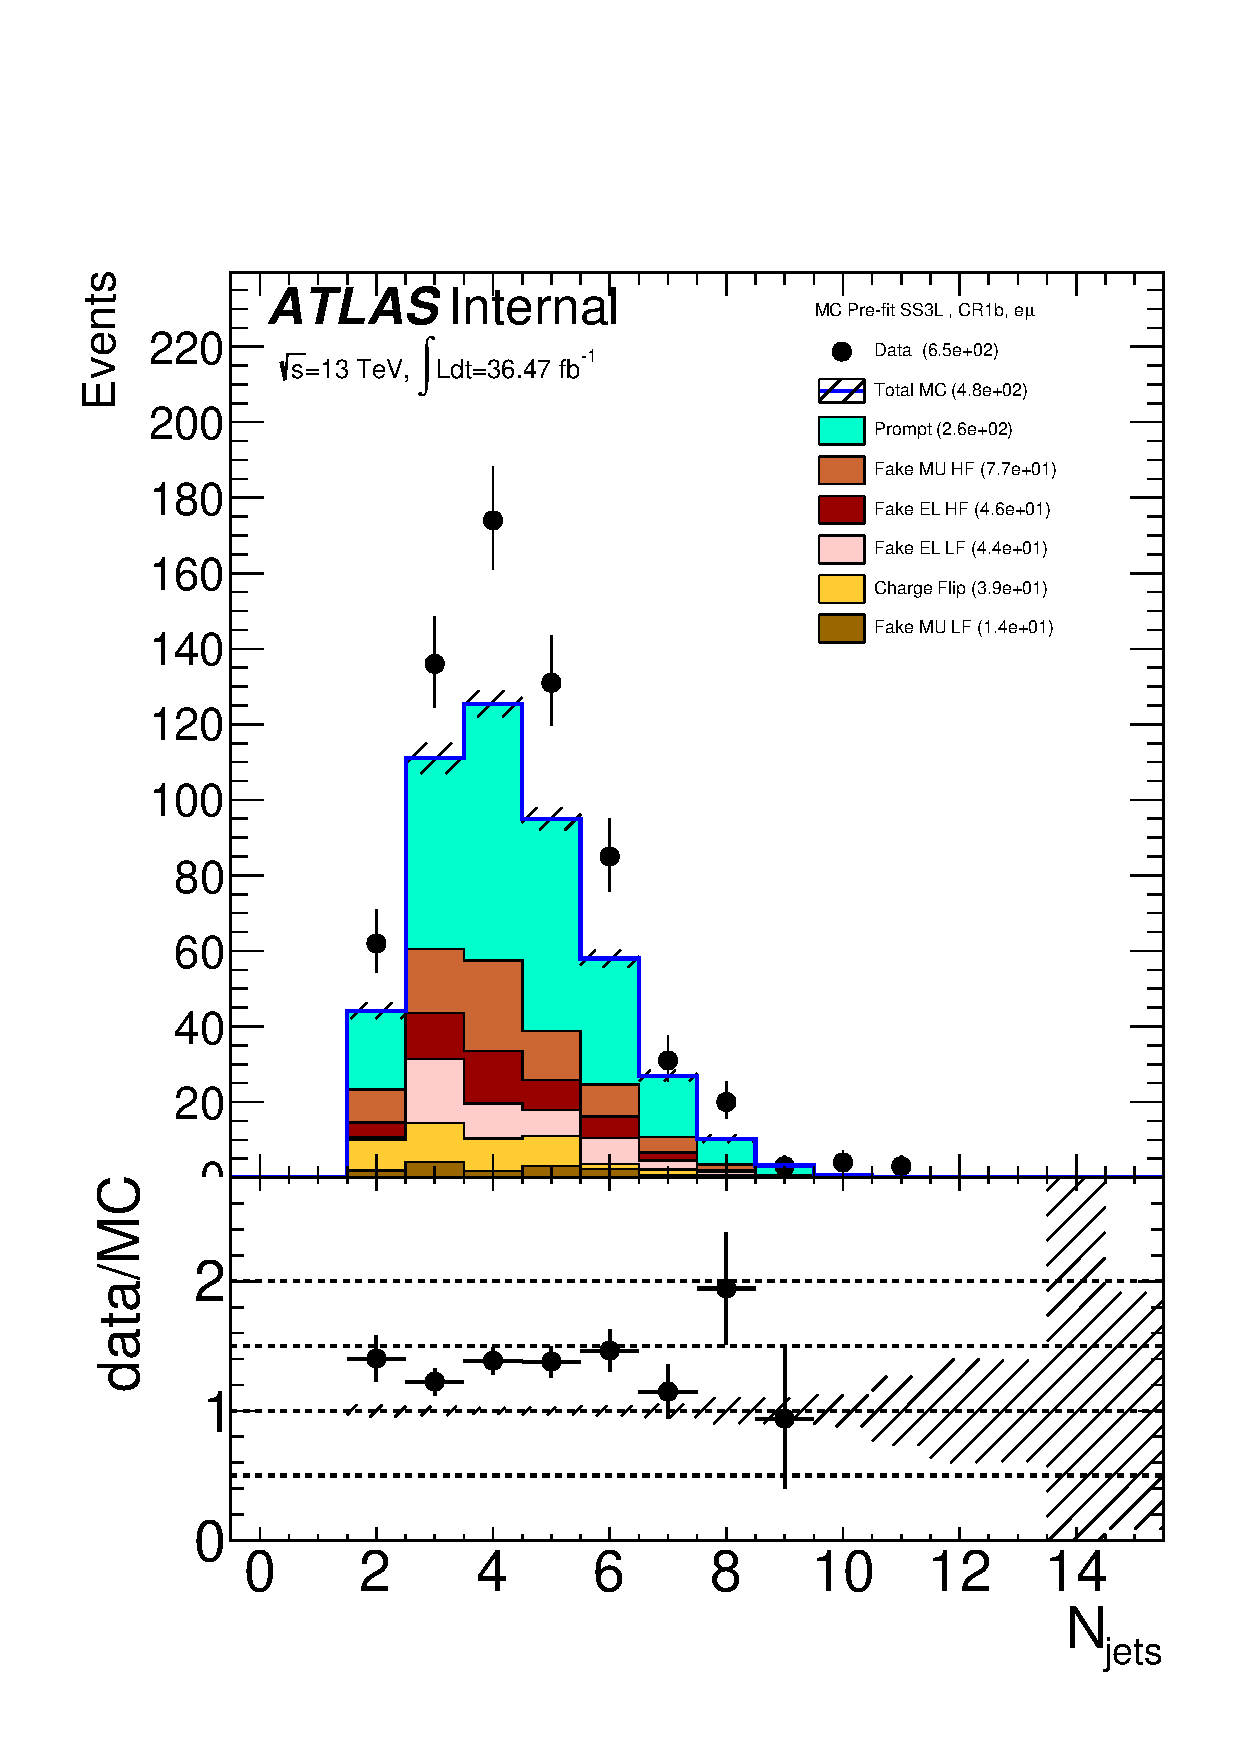
\includegraphics[width=.32\textwidth]{figures/mct/Prefit/NJETS_em_CR1b_SS3L}
   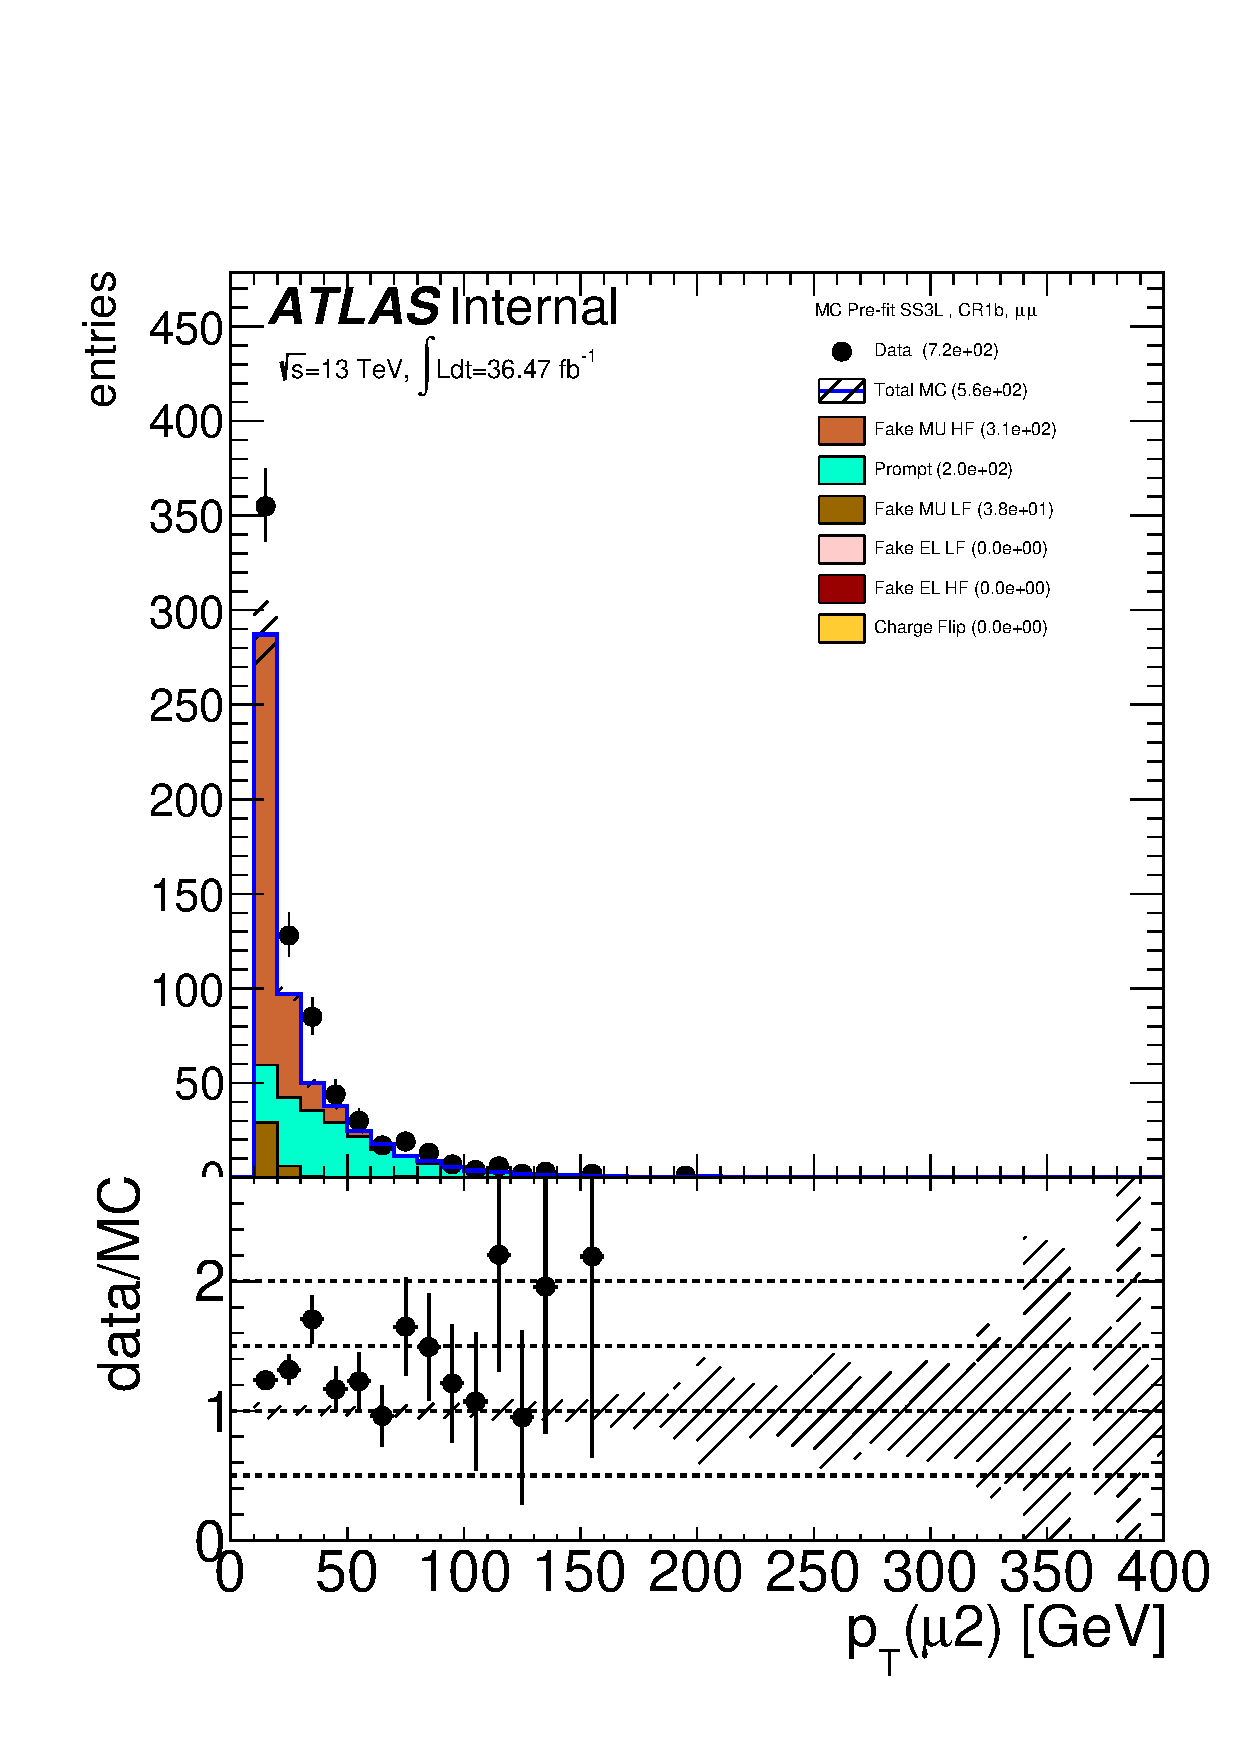
\includegraphics[width=.32\textwidth]{figures/mct/Prefit/mu2_pt_mm_CR1b_SS3L}
 \caption{
 Pre-fit distributions for  $ee$ channel (left), for  $e\mu$ channel (middle), and  for  $\mu\mu$ channel (right) from CR1b that were used in the fit to extract the FNP lepton and charge flip multipliers.
The generator used in these plots is Powheg. The hashed band represents the sum of systematic uncertainties on the predictions.
 \label{f:prefit_CR1b}
 }
 \end{figure}

\begin{figure}[htb]
  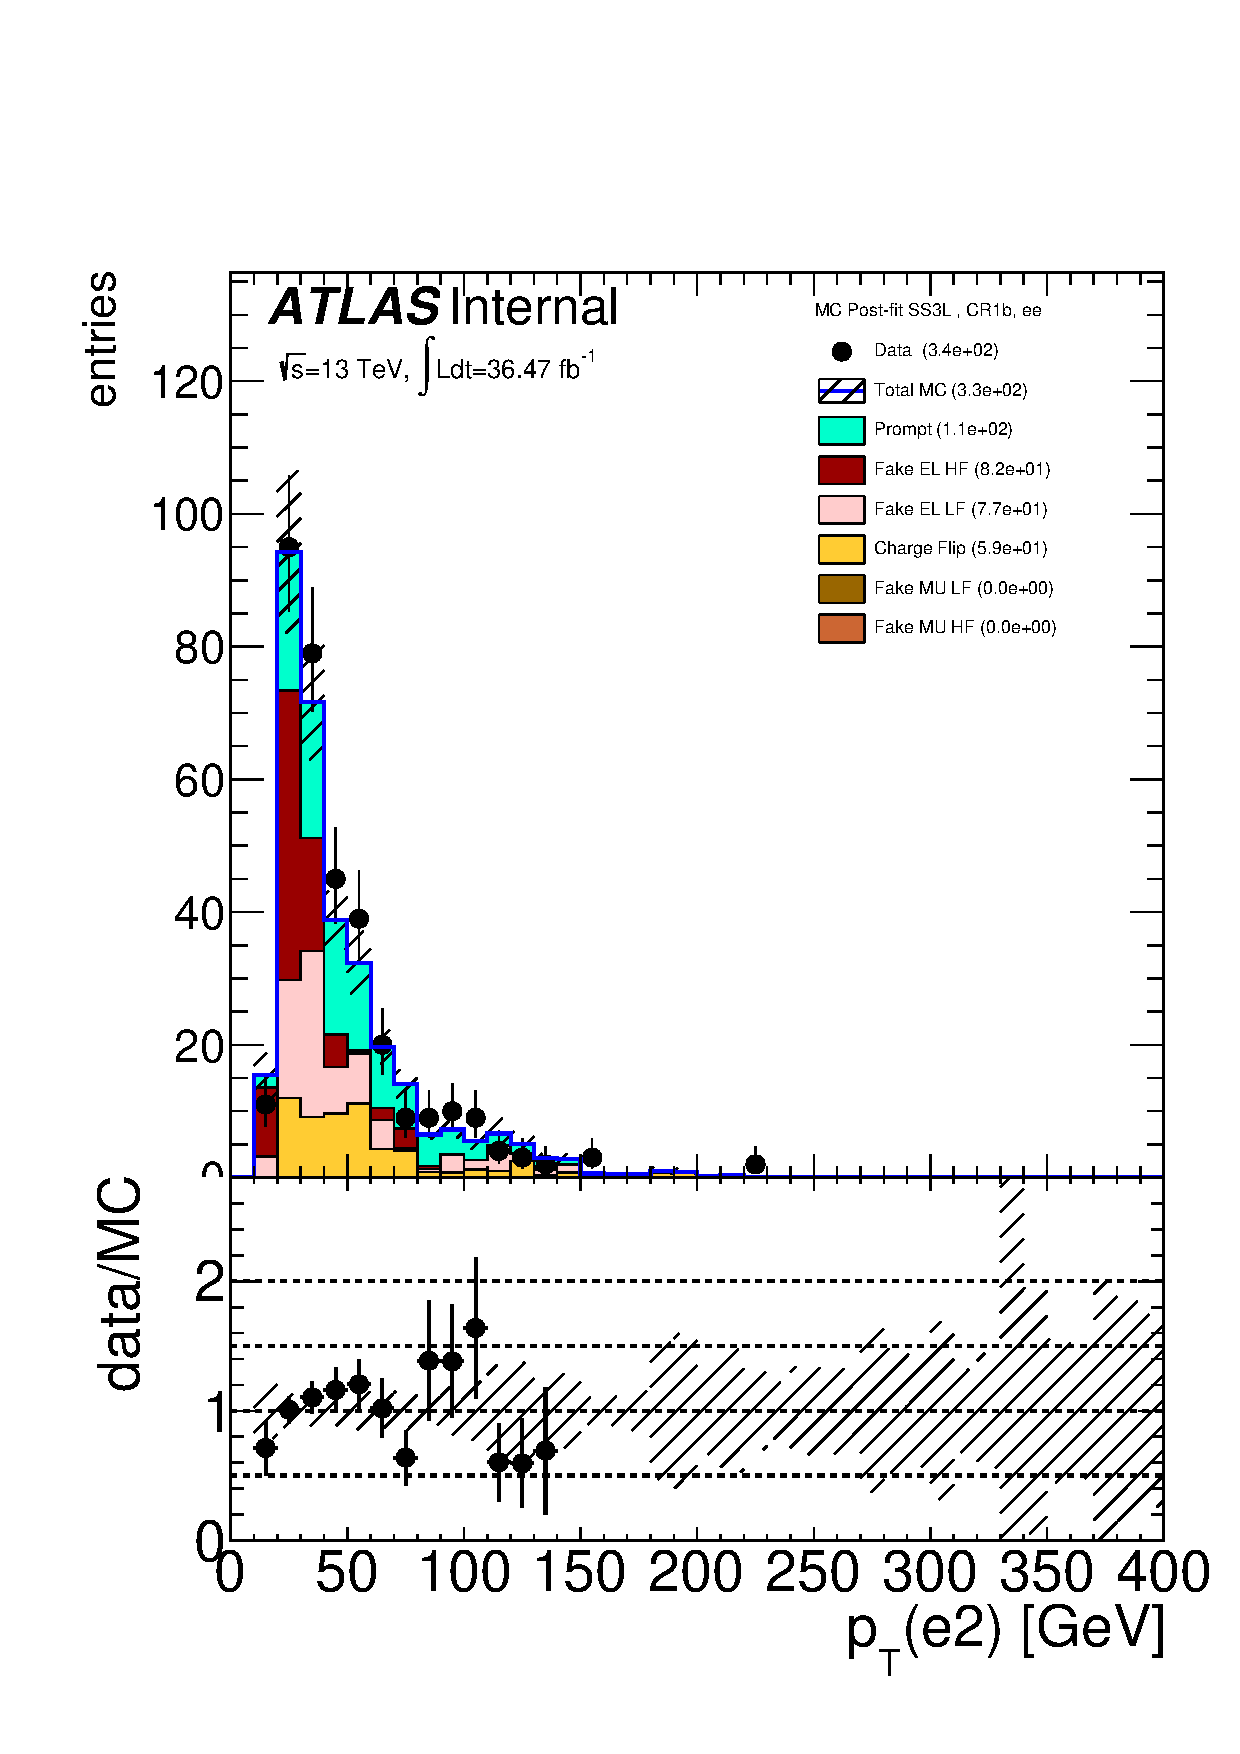
\includegraphics[width=.32\textwidth]{figures/mct/Postfit/el2_pt_ee_CR1b_SS3L}
  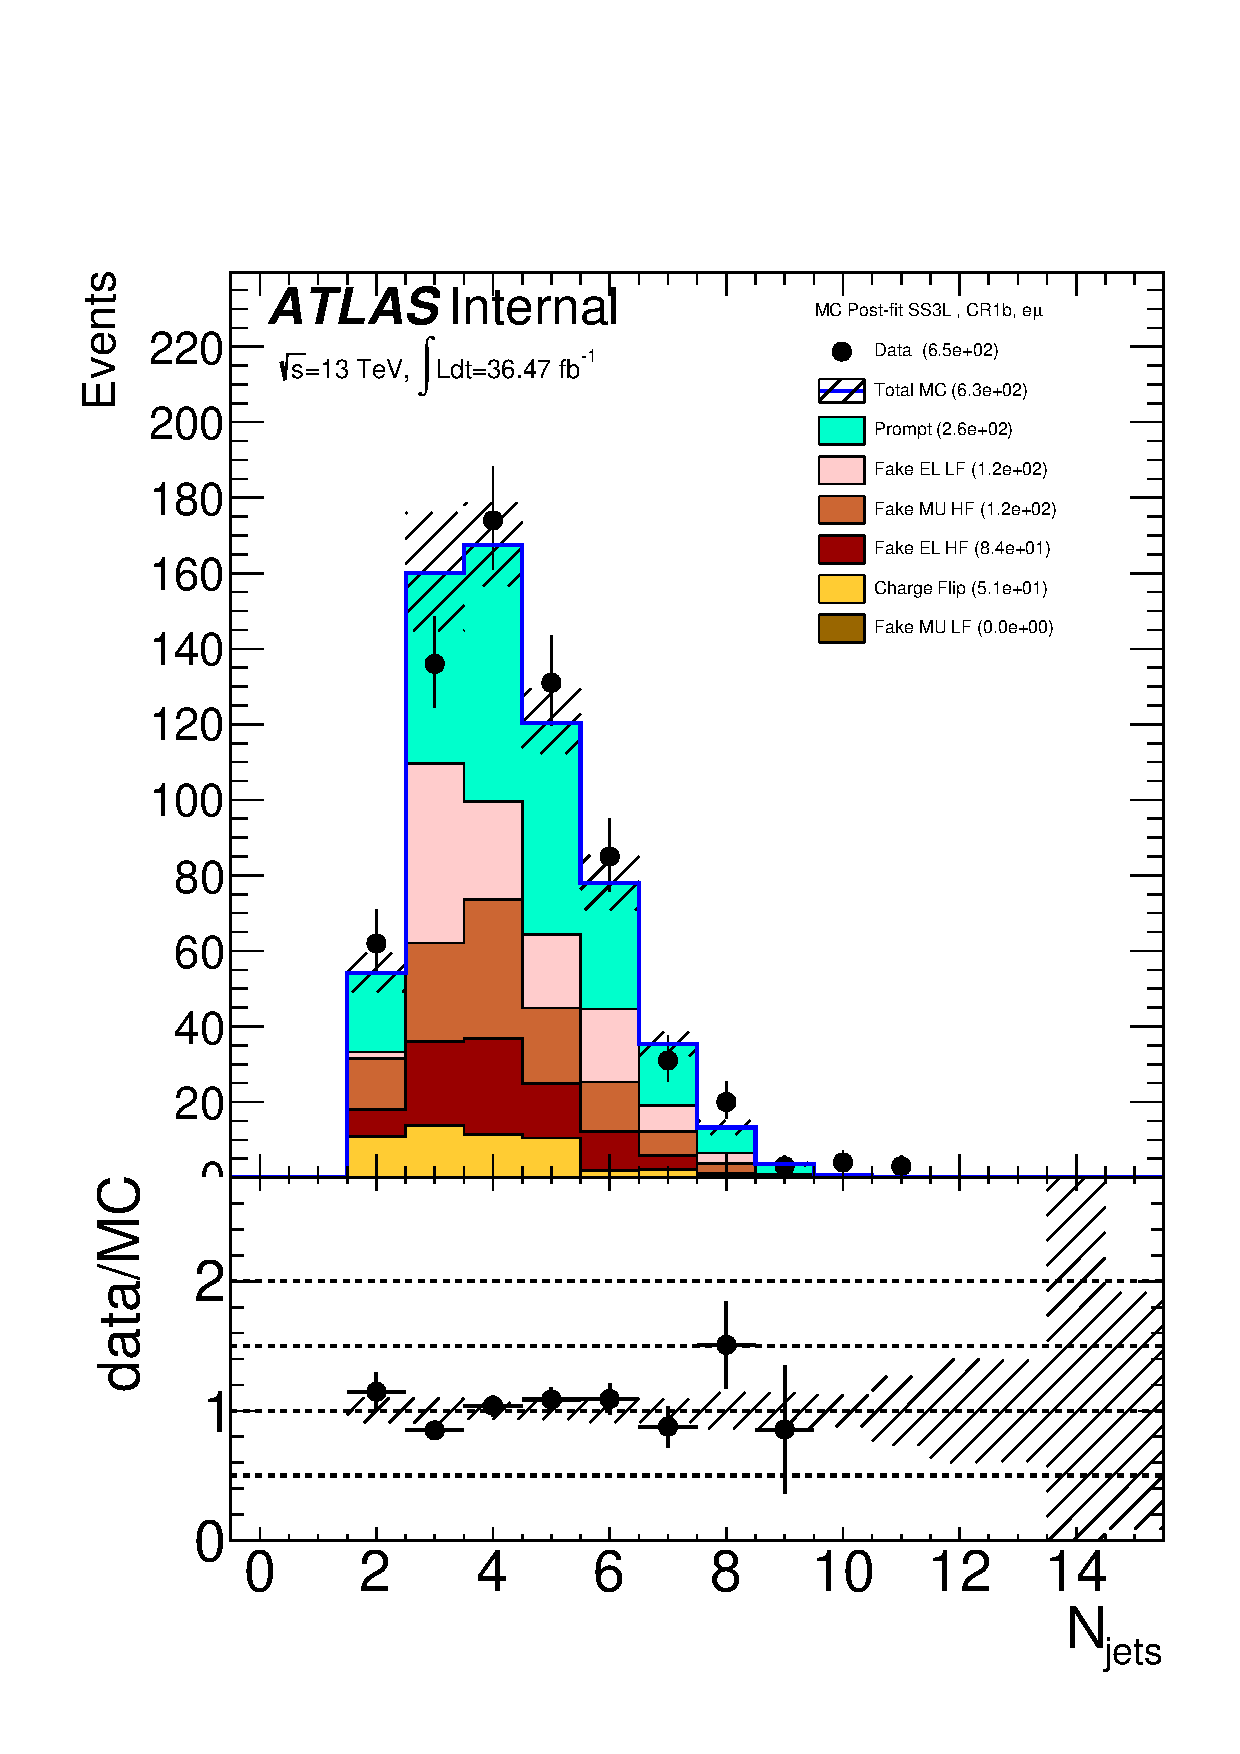
\includegraphics[width=.32\textwidth]{figures/mct/Postfit/NJETS_em_CR1b_SS3L}
  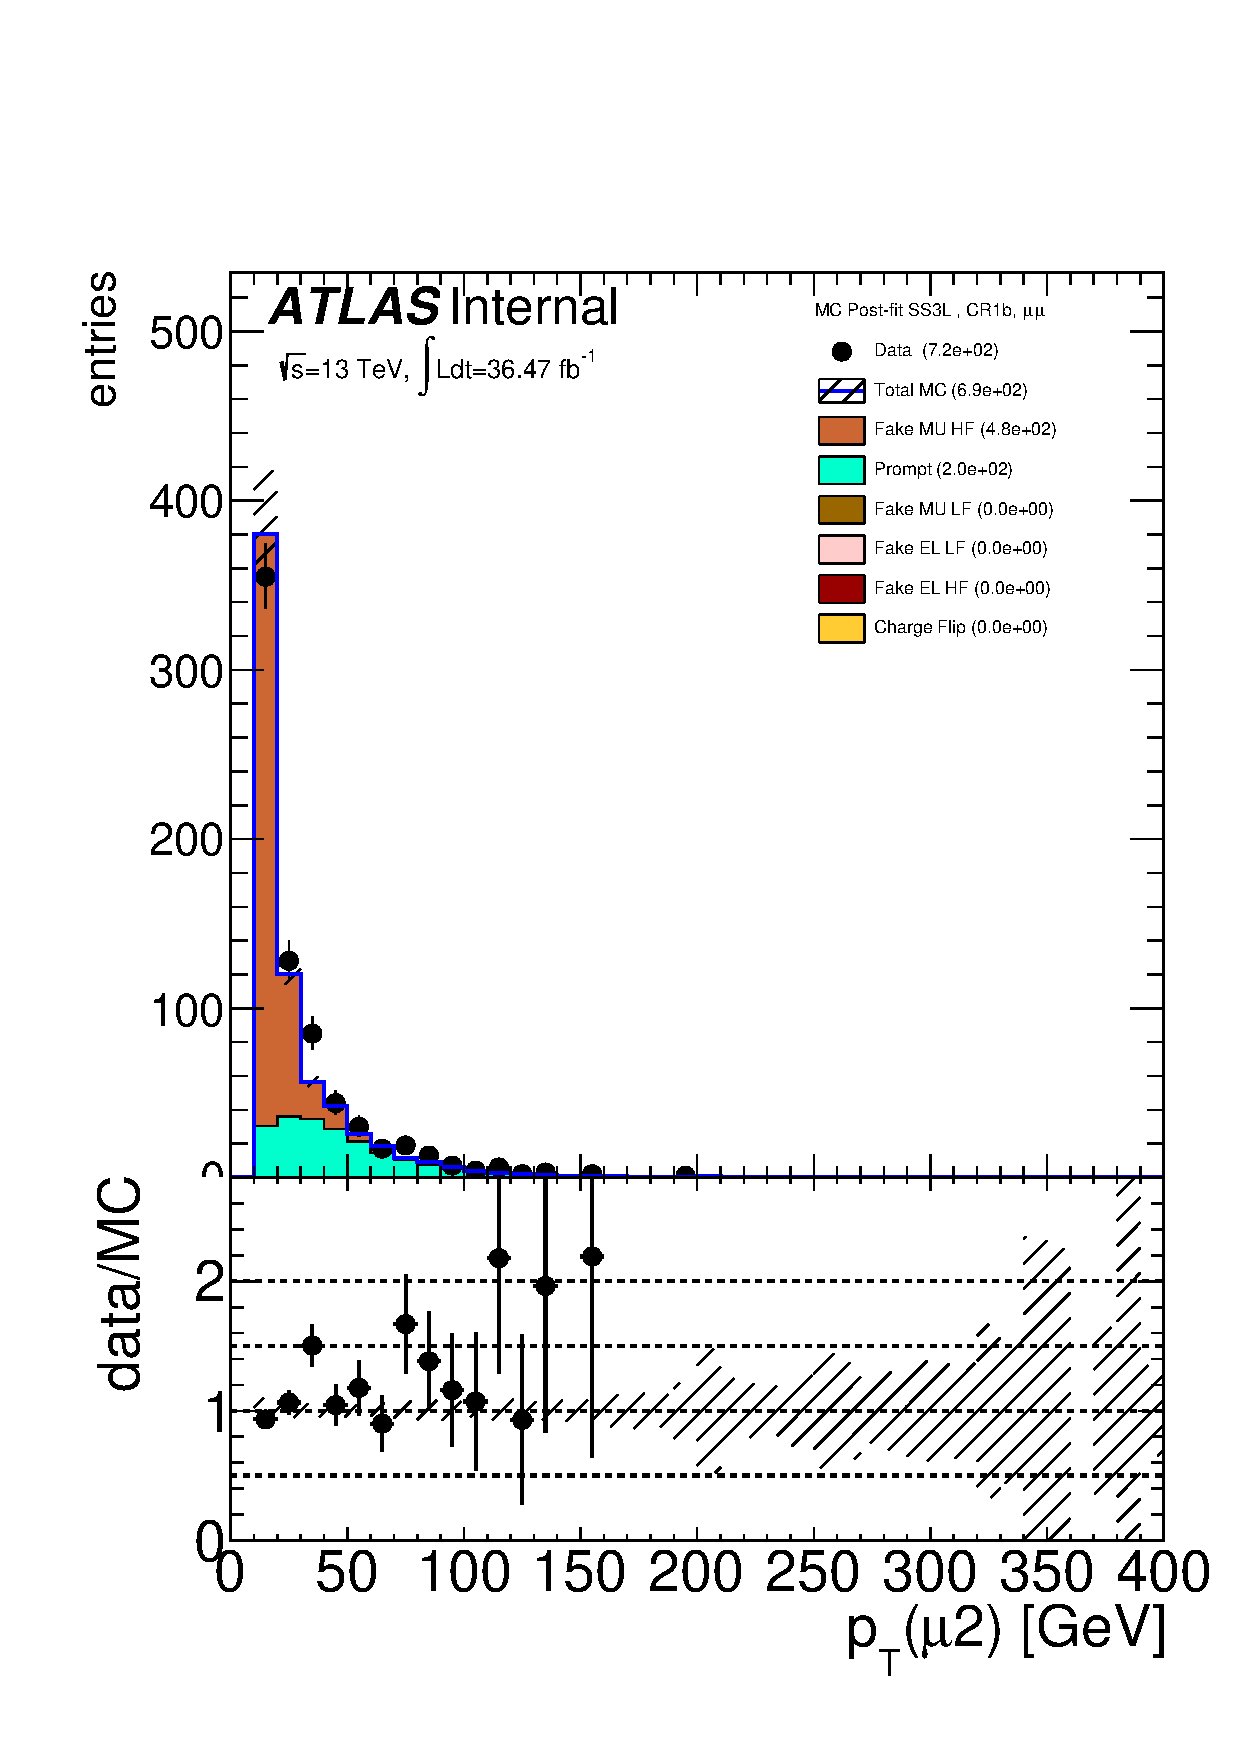
\includegraphics[width=.32\textwidth]{figures/mct/Postfit/mu2_pt_mm_CR1b_SS3L}
\caption{
Post-fit distributions for  $ee$ channel (left), for  $e\mu$ channel (middle), and  for  $\mu\mu$ channel (right) from CR1b that were used in the fit to extract the FNP lepton and charge flip multipliers.
The generator used in these plots is Powheg. The hashed band represents the sum of systematic uncertainties on the predictions.
\label{f:postfit_CR1b}
}
\end{figure}

The minimization of the negative log likelihood using the \textsc{Minuit} package leads 
to the multipliers shown in Tables \ref{t:fake_factors_powheg} and \ref{t:fake_factors_sherpa}.
The tables represent the multipliers obtained from the fit upon using two different parton showers, \POWHEGBOX and \SHERPA 
for the processes that lead to FNP leptons and charge flips.
The systematic uncertainty is obtained by varying the 
generator from \POWHEGBOX to \SHERPA and evaluating the impact on the expected background from FNP and charge flip leptons. 
It is found to be the dominant contribution to the systematic uncertainty of the method (up to 80\%).
The uncertainties in the multipliers themselves correspond to how much the parameter needs to be varied for 
a one standard deviation change in the likelihood function. This uncertainty takes into account the limited number of simulated events and is included as a 
systematic uncertainty on the expected number of background events. 

\begin{table}[htb]
  \caption{The FNP and charge flip multipliers obtained after minimizing the likelihood function using Pythia.
    The uncertainty in the multipliers takes into account the limited statistics of simulated events.
    \label{t:fake_factors_powheg}}
  \centering
  % % \scalebox{0.85}{
   \begin{tabular}{|c|c|c|}
          \hline
          Category & Multiplier & Uncertainty  \\
          \hline
          chFlip & 1.49 & 0.58 \\ 
          HF EL & 2.80 & 0.98 \\
          LF EL & 2.89 & 0.88 \\
          HF MU & 1.59 & 0.31 \\
          LF MU & 1.00 & 1.34 \\
          \hline
        \end{tabular}
  % % }                                                                            
\end{table}

\begin{table}[htb]
  \caption{The FNP and charge flip multipliers obtained after minimizing the likelihood function using Sherpa.
    The uncertainty in the multipliers takes into account the limited statistics of simulated events.
    \label{t:fake_factors_sherpa}}
  \centering
  % % \scalebox{0.85}{
  \begin{tabular}{|c|c|c|}
    \hline
    Category & Multiplier & Uncertainty  \\
    \hline
    chFlip & 1.34 & 0.58 \\ 
    HF EL & 2.40 & 0.85 \\
    LF EL & 1.83 & 1.04 \\
    HF MU & 1.17 & 0.16 \\
    LF MU & 2.40 & 0.81 \\
    \hline
  \end{tabular}                                                                                         
  % % }                                                                            
\end{table}



\section{Matrix Method}


The FNP leptons do not often pass one of the 
lepton selection criteria (identification, impact parameters, and isolations) but have non-zero impact parameter, and are often not 
well-isolated. These selection requirements are key ingredients to control the FNP leptons. 
The number of events with at least one FNP lepton is estimated using two classes of leptons: 
a real-enriched class of ``tight'' leptons corresponding to signal leptons and a fake-enriched class of ``loose'' leptons 
corresponding to candidate leptons with relaxed identification criteria\footnote{Signal leptons are leptons satisfying the signal lepton definition, while the candidate leptons are leptons satisfying some pre-selection cuts and usually passing the overlap removal requirements as discssed in the analysis section ??.}. 
In the next sections, a description of the simplest form of the matrix method will be given with events containing one object. 
Then a generalized treatment that can handle events with an arbitrary number of leptons in the final states will be discussed.

\subsection{Events with one object}

Given the probabilities $\varepsilon/\zeta$ for a real/FNP candidate lepton to satisfy in addition the signal lepton criteria, 
one can relate the number of events with one candidate lepton passing/failing signal requirements ($n_\text{pass}/n_\text{fail}$) to the number of events with one real/FNP signal leptons ($n_\text{real}/n_\text{FNP}$):

\begin{align}
\begin{pmatrix}n_\text{pass}\\n_\text{fail}\end{pmatrix} 
= \begin{pmatrix}1 & 1\\ \frac{1-\varepsilon}\varepsilon & \frac{1-\zeta}\zeta\end{pmatrix}
\begin{pmatrix}n_\text{real}\\n_\text{FNP}\end{pmatrix}; 
\label{eqn:matrix_method}
\end{align}
allowing to determine the unknown number of events $n_\text{FNP}$ from the observed $n_\text{pass}$ and $n_\text{fail}$. 

\subsection{Dynamic matrix method}


This readily generalizes to events with more than one lepton, with a formalism described in details.
An implementation of this formalism (known also as the dynamic or generalized matrix method) can handle an arbitrary number of leptons 
in the event. 
The method should be applied event-by-event, effectively resulting into a weight being assigned to each event. The predicted yield of 
events with FNP leptons is simply the sum of weights.


The application of the matrix method to multilepton final states comes with two specificities. Firstly, contributions of events with charge-flip electrons would bias a straightforward matrix method estimate (in particular for a final state formed by two leptons with same electric charge). This happens because the candidate-to-signal efficiency for such electrons is typically lower than for real electrons having a correctly-assigned charge. One therefore needs to subtract from $n_\text{pass}$ and $n_\text{fail}$ the estimated contributions from charge-flip. This can be performed by including as well events with pairs of opposite-sign candidate leptons in the matrix method estimate, but assigning them an extra weight corresponding to the charge-flip weight. Thanks (again) to the linearity of the matrix method with respect to $n_\text{pass}$ and $n_\text{fail}$, this weight-based procedure is completely equivalent (but more practical) to the aforementioned subtraction. 

Secondly, the analytic expression of the matrix method event weight depends on the lepton multiplicity of the final state. This concerns events with three or more candidate leptons: one such event takes part both in the evaluation of the FNP lepton background for a selection with two signal leptons or a selection with three signal leptons, but with different weights\footnote{This can appear for inclusive selections: for example an event with two signal leptons may or not contain additional candidate leptons, in a transparent way}. Therefore, for a given event used as input to the matrix method, one should consider all possible leptons combinations, each with its own weight and its own set of kinematic variables. For example, a $e^+e^-\mu^+$ event is comptabilized in the background estimate both as an $e^+\mu^+$ event (with a weight w1) and as an $e^+e^-\mu^+$ event (with a weight $w_2\neq w1$).  

\subsection{Propagation of uncertainties}

The two parameters ($\varepsilon$ and $\zeta$ respectively) can be measured in data, and depend on the flavor and kinematics of the involved leptons.  Systematic uncertainties resulting from the measurement of these two parameters, and their extrapolation to the signal regions, can be propagated to uncertainties on the event weight through standard first-order approximations. The different sources of uncertainties should be tracked separately so that correlations of uncertainties across different events can be accounted for correctly. The resulting set of uncertainties on the cumulated event weights can be then added in quadrature to form the systematic uncertainty on the predicted FNP lepton background yield. The corresponding statistical uncertainty can be taken as the RMS of the event weights.


\section{Real lepton efficiency}
\graphicspath{{figures/real_lepton_efficiency/}}
The real lepton efficiency parameter should be measured in a region dominated by real leptons, usually with the same topology as the real leptons dominating the signal regions. It can be a control region dominated by $Z\to\ell\ell$ or ``$W\to\ell\nu$'' or \ttbar, etc. events.
This section is dedicated to the real lepton efficiency measurement using the Tag and Probe method. 
The real efficiency is obtained by taking the ratio between the number of probe leptons passing the signal requirement 
($n_\mathrm{signal}$) and the number of probe candidate leptons ($n_\mathrm{candidate}$).
The estimated number of the background events ($N_\mathrm{candidate}^{bkg}$) associated with the low $p_\mathrm{T}$ leptons 
(as low as 20 \GeV) are considered and estimated using a background template method.
Equation~\ref{eq:RLE_efficiency_formula} shows the real lepton efficiency calculation.

\begin{equation}
\epsilon = \frac{N_{\mathrm{signal}}}{N_{\mathrm{candidate}} - N_{\mathrm{candidate}}^{bkg}}
\label{eq:RLE_efficiency_formula}
\end{equation}

%%%
\subsection{The $Z$ tag-and-probe method}
\label{subsubsec:RLE_ZTandP_method}

The leptons used for the efficiency measurements are extracted from data using the $Z$ tag-and-probe method.
Events are required to have at least two candidate leptons.
One of the two leptons, the tag lepton, is required to have a transverse momentum $\pt>25 \GeV$ and pass the signal lepton requirements
specified in Table ??.
In the case of the $Z\to ee$ events, an additional $|\eta|<2$ requirement is used for the tag and probe selection.
The probe lepton, which is used for the real efficiency measurements, is required to pass the candidate lepton requirements and have to 
carry opposite charge and same flavor with respect to the corresponding tag lepton. This requirement ensures the selection of 
real leptons to allow the real lepton efficiency measurement.
The tag and the probe leptons are required to match the single lepton triggers or dilepton triggers listed in 
Table~\ref{tab:RLE_single_lepton_triggers}.

\begin{table}[htbp]
\begin{center}
\begin{tabular}{cccc}
\hline
\hline
Trigger & lepton & 2015 & 2016\\
\hline
\multirow{2}{*}{Single lepton trigger} & electron & \texttt{e24\_lhmedium\_iloose\_L1EM20VH} & \texttt{e26\_lhtight\_nod0\_ivarloose}\\
& muon & \texttt{mu20\_iloose\_L1MU15} & \texttt{mu26\_ivarmedium}\\
\hline
\multirow{2}{*}{Dilepton trigger} & electron & \texttt{2e12\_lhloose\_L12EM10VH} & \texttt{2e17\_lhvloose\_nod0}\\
& muon & \texttt{mu18\_mu8noL1} & \texttt{mu22\_mu8noL1}\\
\hline
\hline
\end{tabular}
\end{center}
\caption{The list of single lepton and dilepton triggers used for the real lepton efficiency measurements.
The dilepton triggers are used for studying the systematic uncertainties causing by the trigger.}
\label{tab:RLE_single_lepton_triggers}
\end{table}

All possible combinations of the tag-and-probe pairs are considered to avoid any bias and to increase the statistics.
The invariant mass of the tag-and-probe pair system should satisfy $80<m_{\ell\ell}<100 \GeV$.
The data-to-MC comparison of the tag-and-probe pair invariant mass distributions are shown in Figure~\ref{fig:RLE_mll_distributions}, and indicates the need of subtracting the background, especially when the probe electron has $\pt<20 \GeV$.

\begin{figure}[htbp]
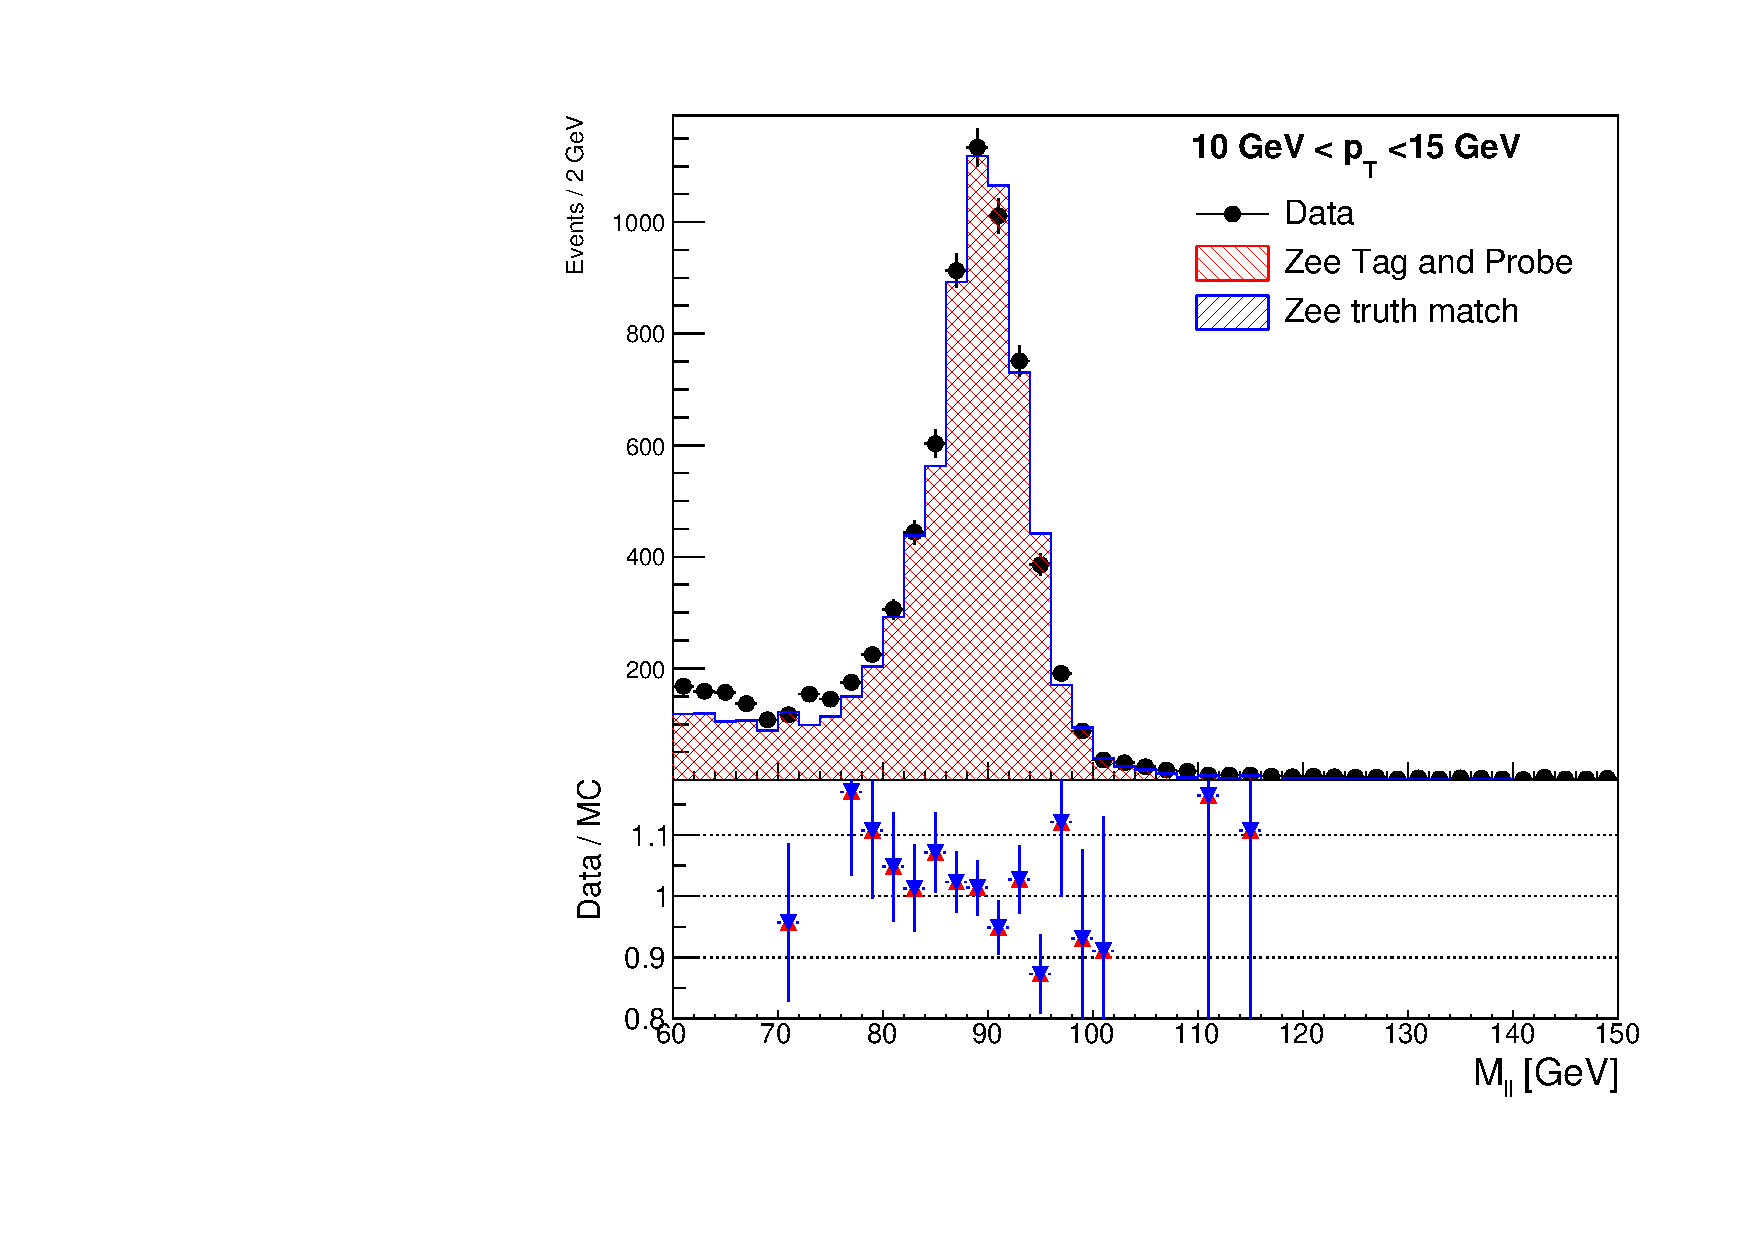
\includegraphics[width=0.48\textwidth]{signal_level_Mee_pt1015_ratio_plot_MC_normalized}
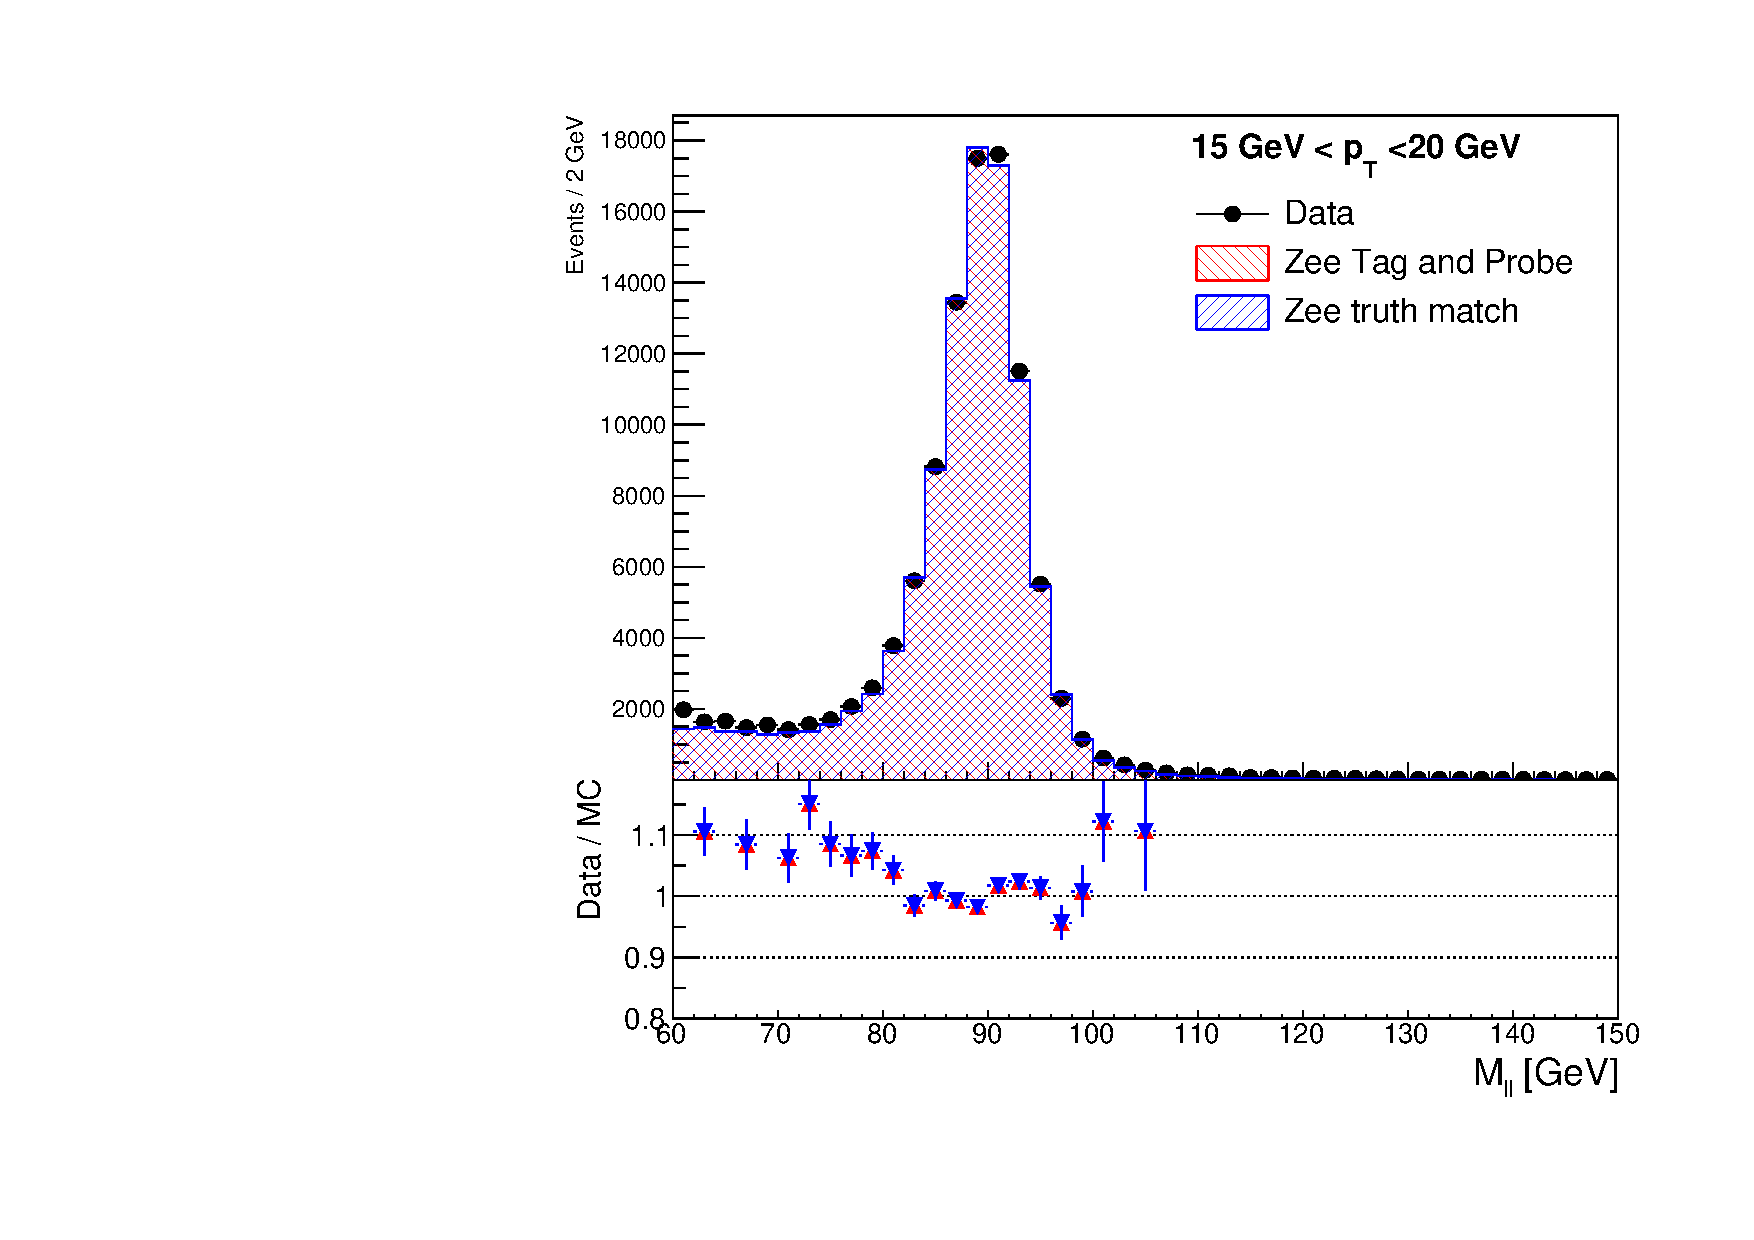
\includegraphics[width=0.48\textwidth]{signal_level_Mee_pt1520_ratio_plot_MC_normalized}\\
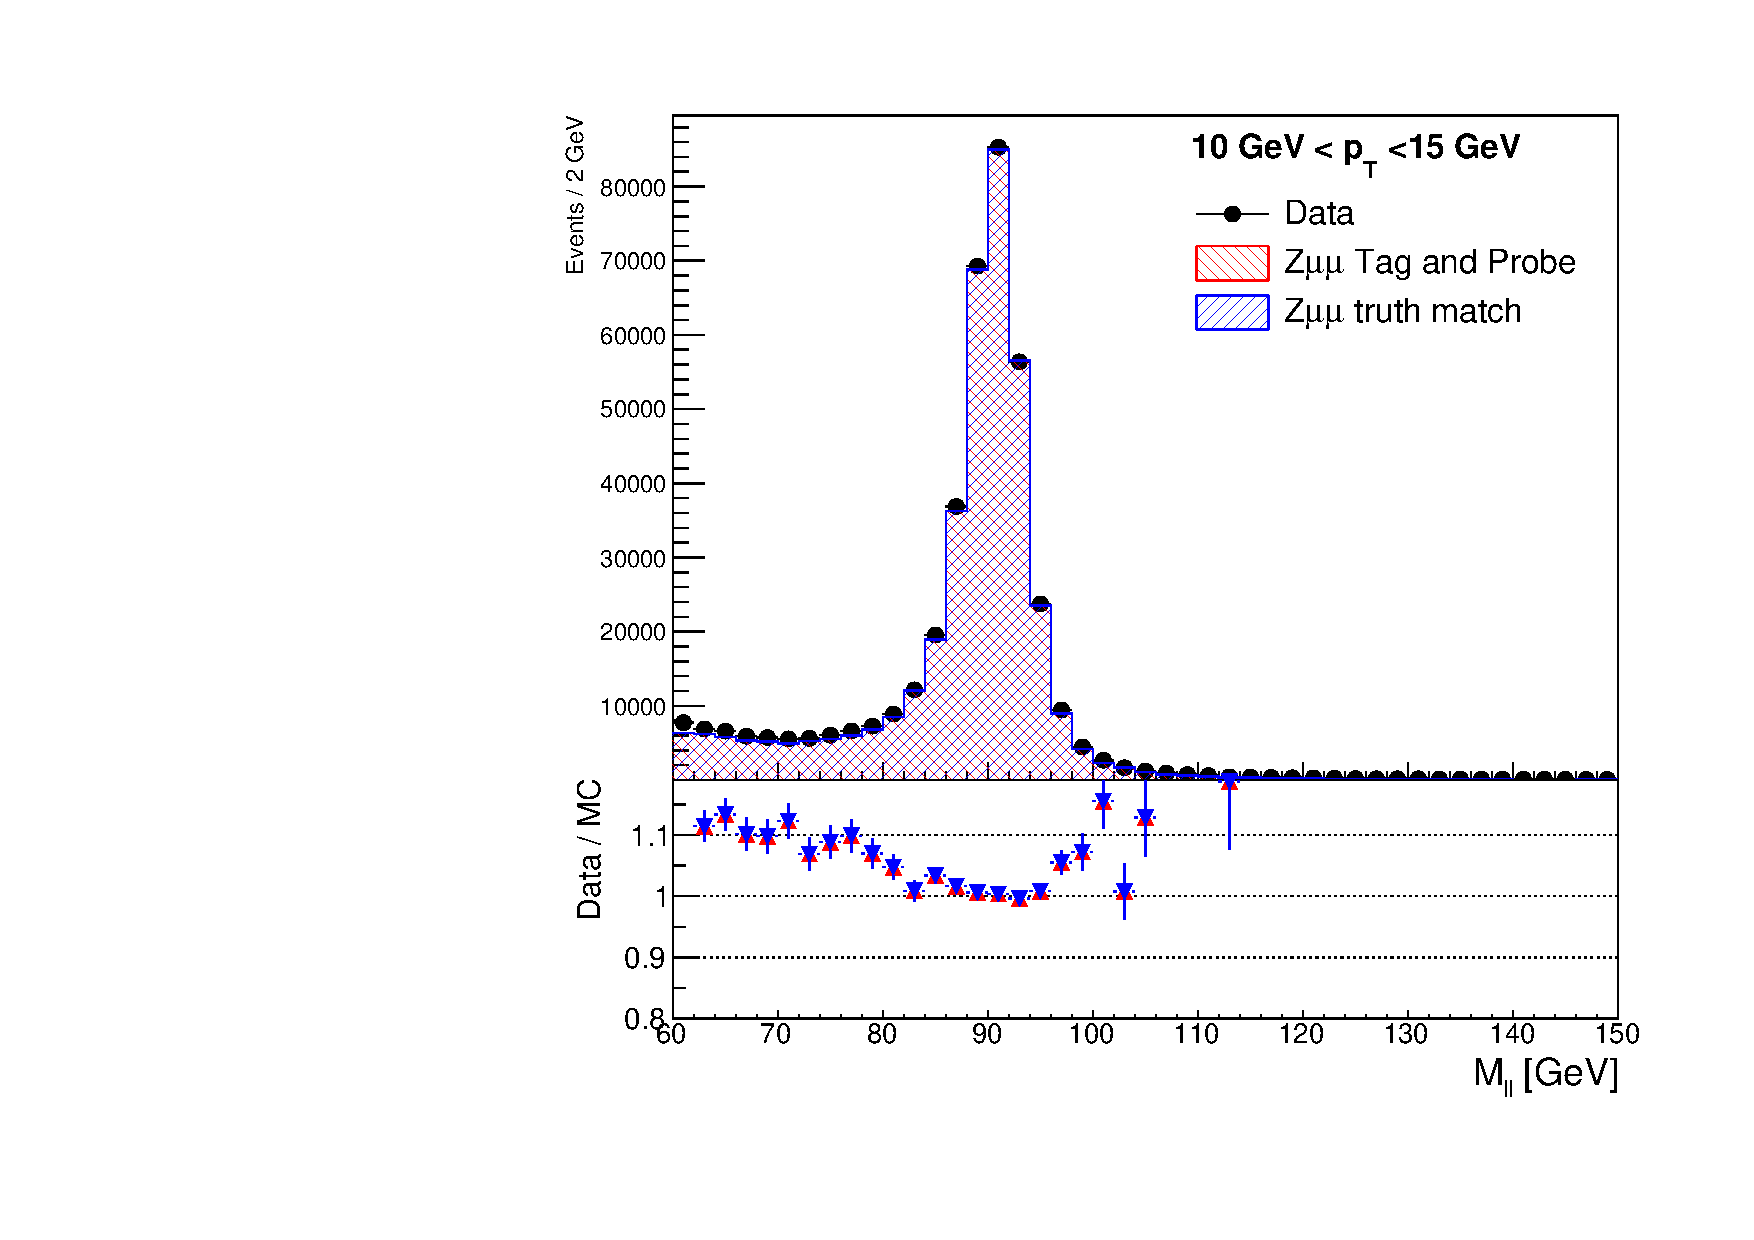
\includegraphics[width=0.48\textwidth]{signal_level_Mmumu_pt1015_ratio_plot_MC_normalized}
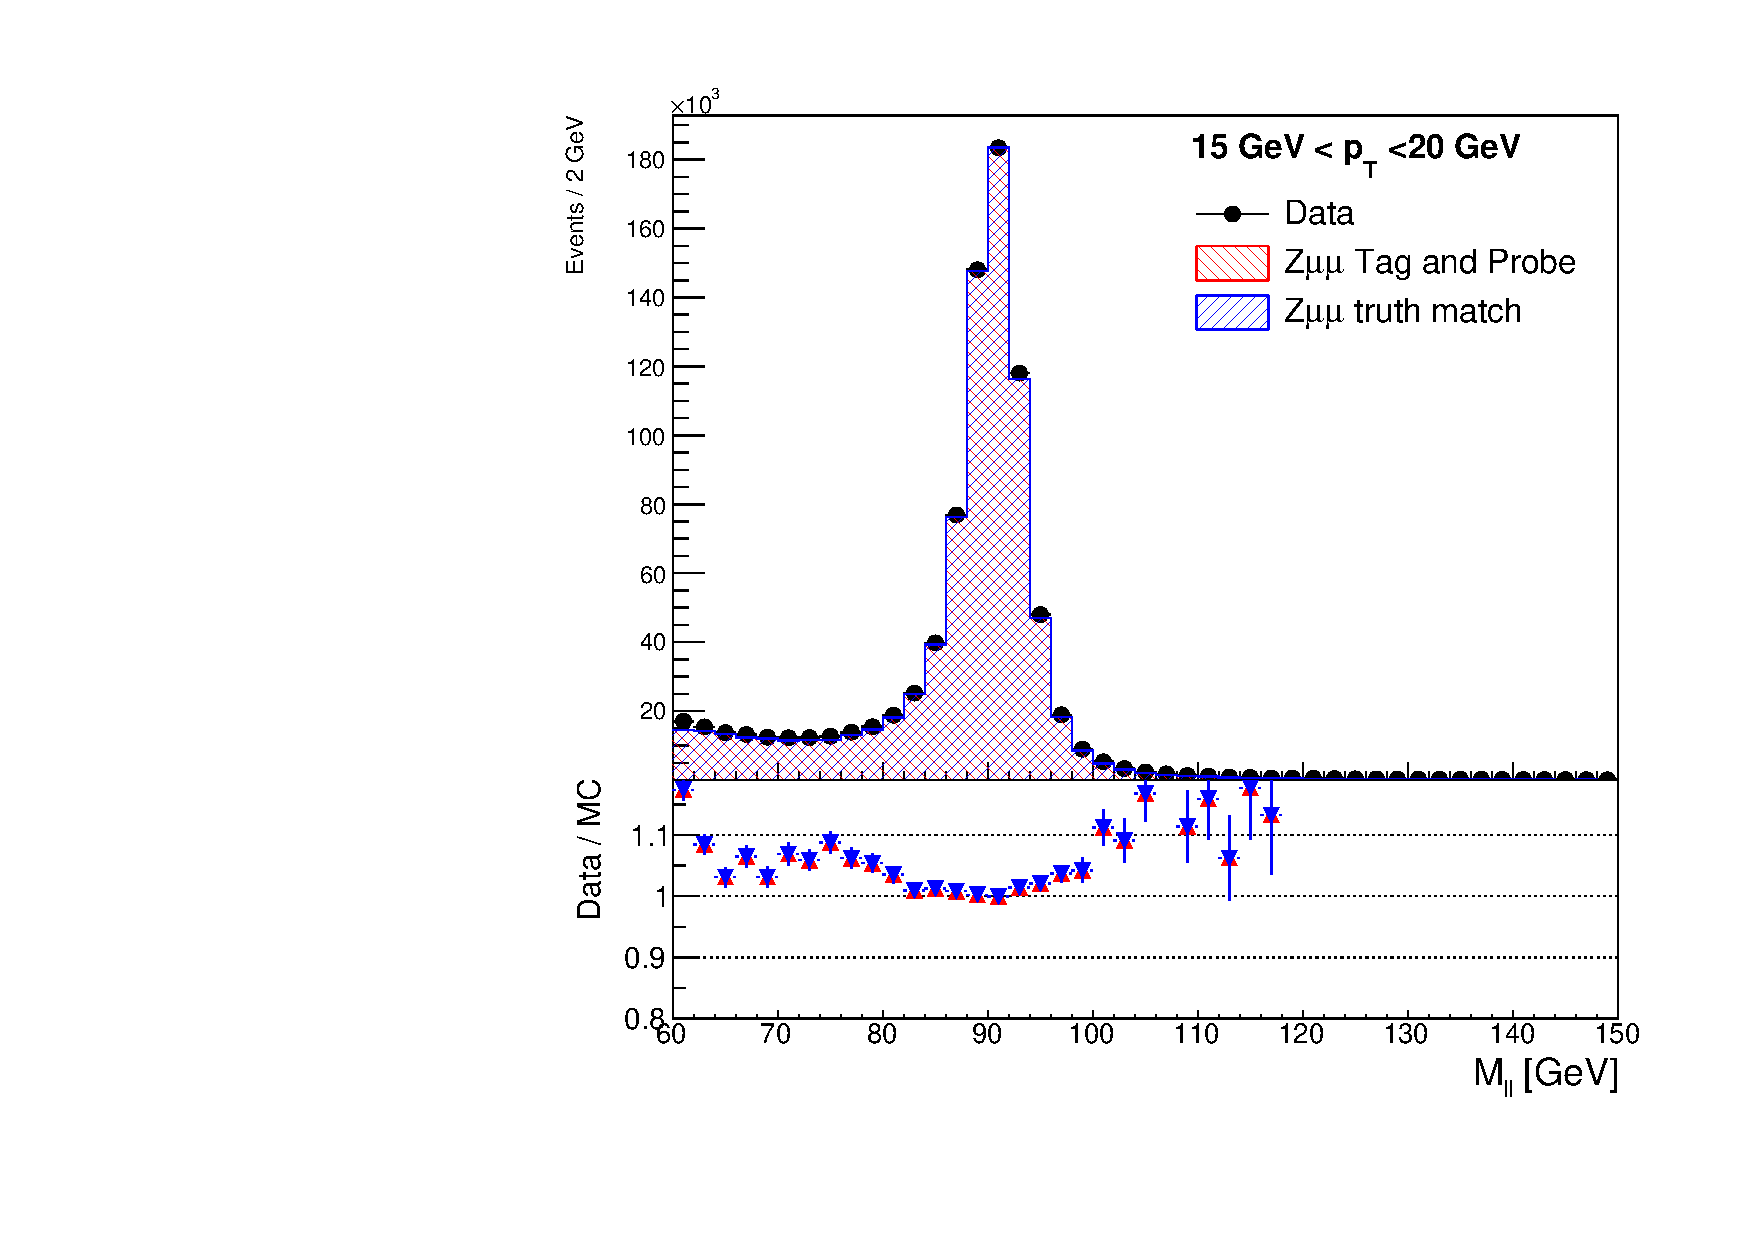
\includegraphics[width=0.48\textwidth]{signal_level_Mmumu_pt1520_ratio_plot_MC_normalized}
\caption{The distributions of the tag-and-probe pair invariant mass ($m_{\ell\ell}$) computed using $Z+jets$ MC and 2015 + 2016 data.
The blue color represents the $Z$ truth matched events, the red color stands for the $Z$ tag-and-probe events, and the black dots are data.
The top row shows the $m_{ee}$ computed with probe electrons in the $10<\pt<15 \GeV$ (left) and $15<\pt<20 \GeV$ (right) intervals.
The bottom row shows the $m_{\mu\mu}$ cases.
The MC distributions are scaled to the data using a Gaussian fit of the $Z$ mass peak ($85<m_{\ell\ell}<95 \GeV$).}
\label{fig:RLE_mll_distributions}
\end{figure}

The background contamination associated with these low $\pt$ electrons is estimated using a background template method similar to the one used by the $e/\gamma$ performance group for their efficiency measurements~\cite{ATLAS-CONF-2014-018}.
Because the real lepton efficiency is obtained by computing the ratio between the number of probe leptons passing the signal requirements ($N_{\textrm{signal}}$) and the number of probe leptons passing the candidate requirements ($N_{\textrm{candidate}}$), the estimated background contamination ($N_{\textrm{candidate}}^{bkg}$) in the candidate probe leptons needs to be subtracted.
As the background contamination is found to be negligible for signal leptons, no background subtraction is performed at the numerator.
Equation~\ref{eq:RLE_efficiency_formula} shows the real lepton efficiency calculation.

\begin{equation}
\epsilon = \frac{N_{\textrm{signal}}}{N_{\textrm{candidate}} - N_{\textrm{candidate}}^{bkg}}
\label{eq:RLE_efficiency_formula}
\end{equation}



\subsection{>Background subtraction}
\label{subsubsec:RLE_bkg_contamination}

The background contamination has been evaluated on data using a background template method.
A sample enriched in background is obtained by inverting the calorimeter isolation and track isolation cuts and requesting the electron object to fail the medium LH identification.
In order to asses a systematic on the background template definition, three variations of background template definitions are considered.
Table~\ref{tab:RLE_bkg_templates} summarizes the background template definitions and the Figure~\ref{fig:RLE_bkg_templates} shows the background template $m_{ee}$ distributions computed with probe electrons in $10<\pt<15 \GeV$ and $15<\pt<20 \GeV$, respectively.
The invariant mass distribution of the template events ($m_{ee}^{\textrm{template}}$) is then used to estimate the amount of background in the measurement region ($80<m_{\ell\ell}<100 \GeV$).

\begin{table}[htbp]
\begin{center}
\begin{tabular}{cccc}
\hline
\hline
cut & variation 1 template & candidate template & variation 2 template\\
\hline
Identification & - & fail medium LH & fail medium LH\\
Calorimeter isolation & $E_{\text T}^{topocone20} /\pt>6\%$ & $E_{\text T}^{topocone20} /\pt>15\%$ & $E_{\text T}^{topocone20} /\pt>20\%$\\
Track isolation & $p_{\text T}^{varcone20} /\pt>6\%$ & $E_{\text T}^{topocone20} /\pt>8\%$ & $E_{\text T}^{topocone20} /\pt>15\%$\\
\hline
\hline
\end{tabular}
\end{center}
\caption{The definition of the background templates used to estimate the background contamination associated with the $Z$ tag-and-probe method.
The candidate template is used to estimate the background contamination and the variation 1 and 2 templates, which have looser and tighter requirements, are used to assess the systematic caused by the background contamination.}
\label{tab:RLE_bkg_templates}
\end{table}

\begin{figure}[htbp]
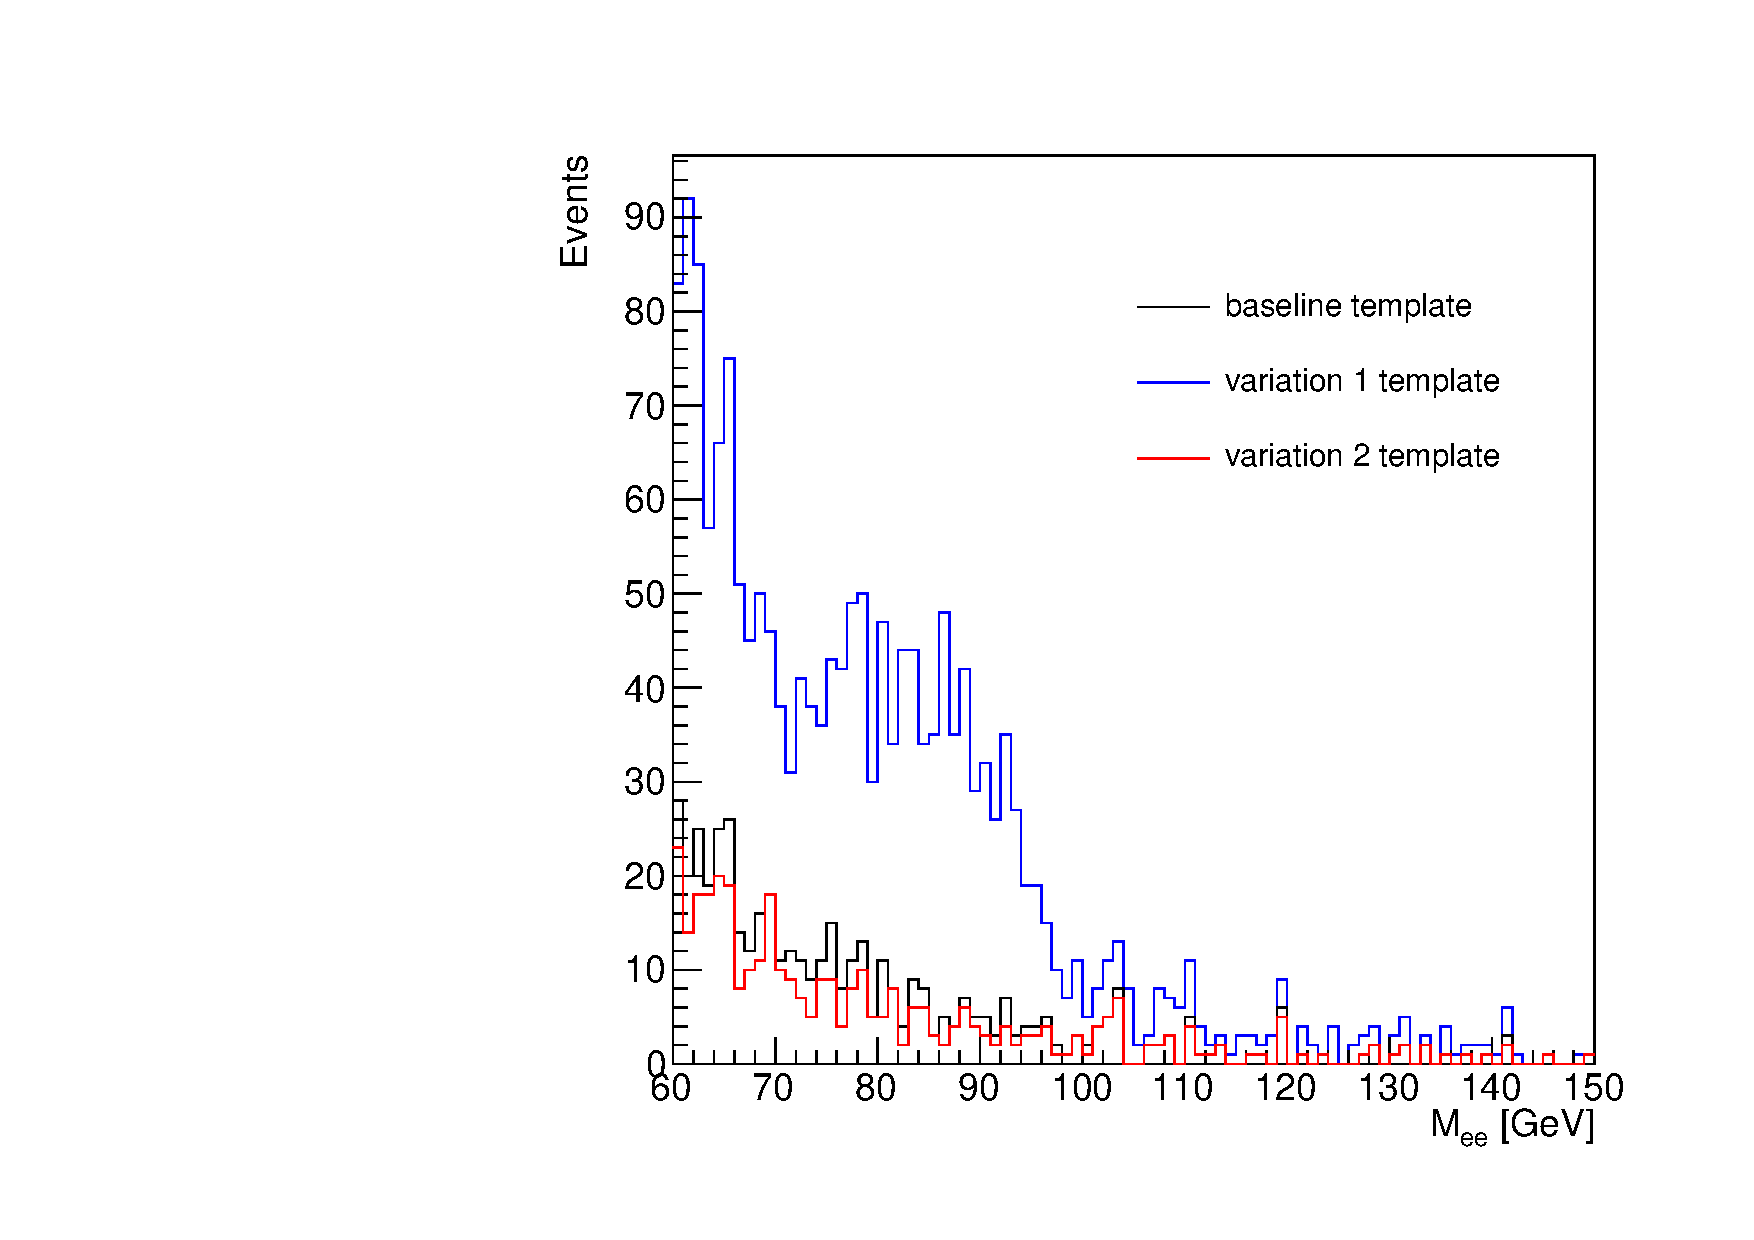
\includegraphics[width=0.48\textwidth]{bkg_template_electron_pt_1015_eta0201.pdf}
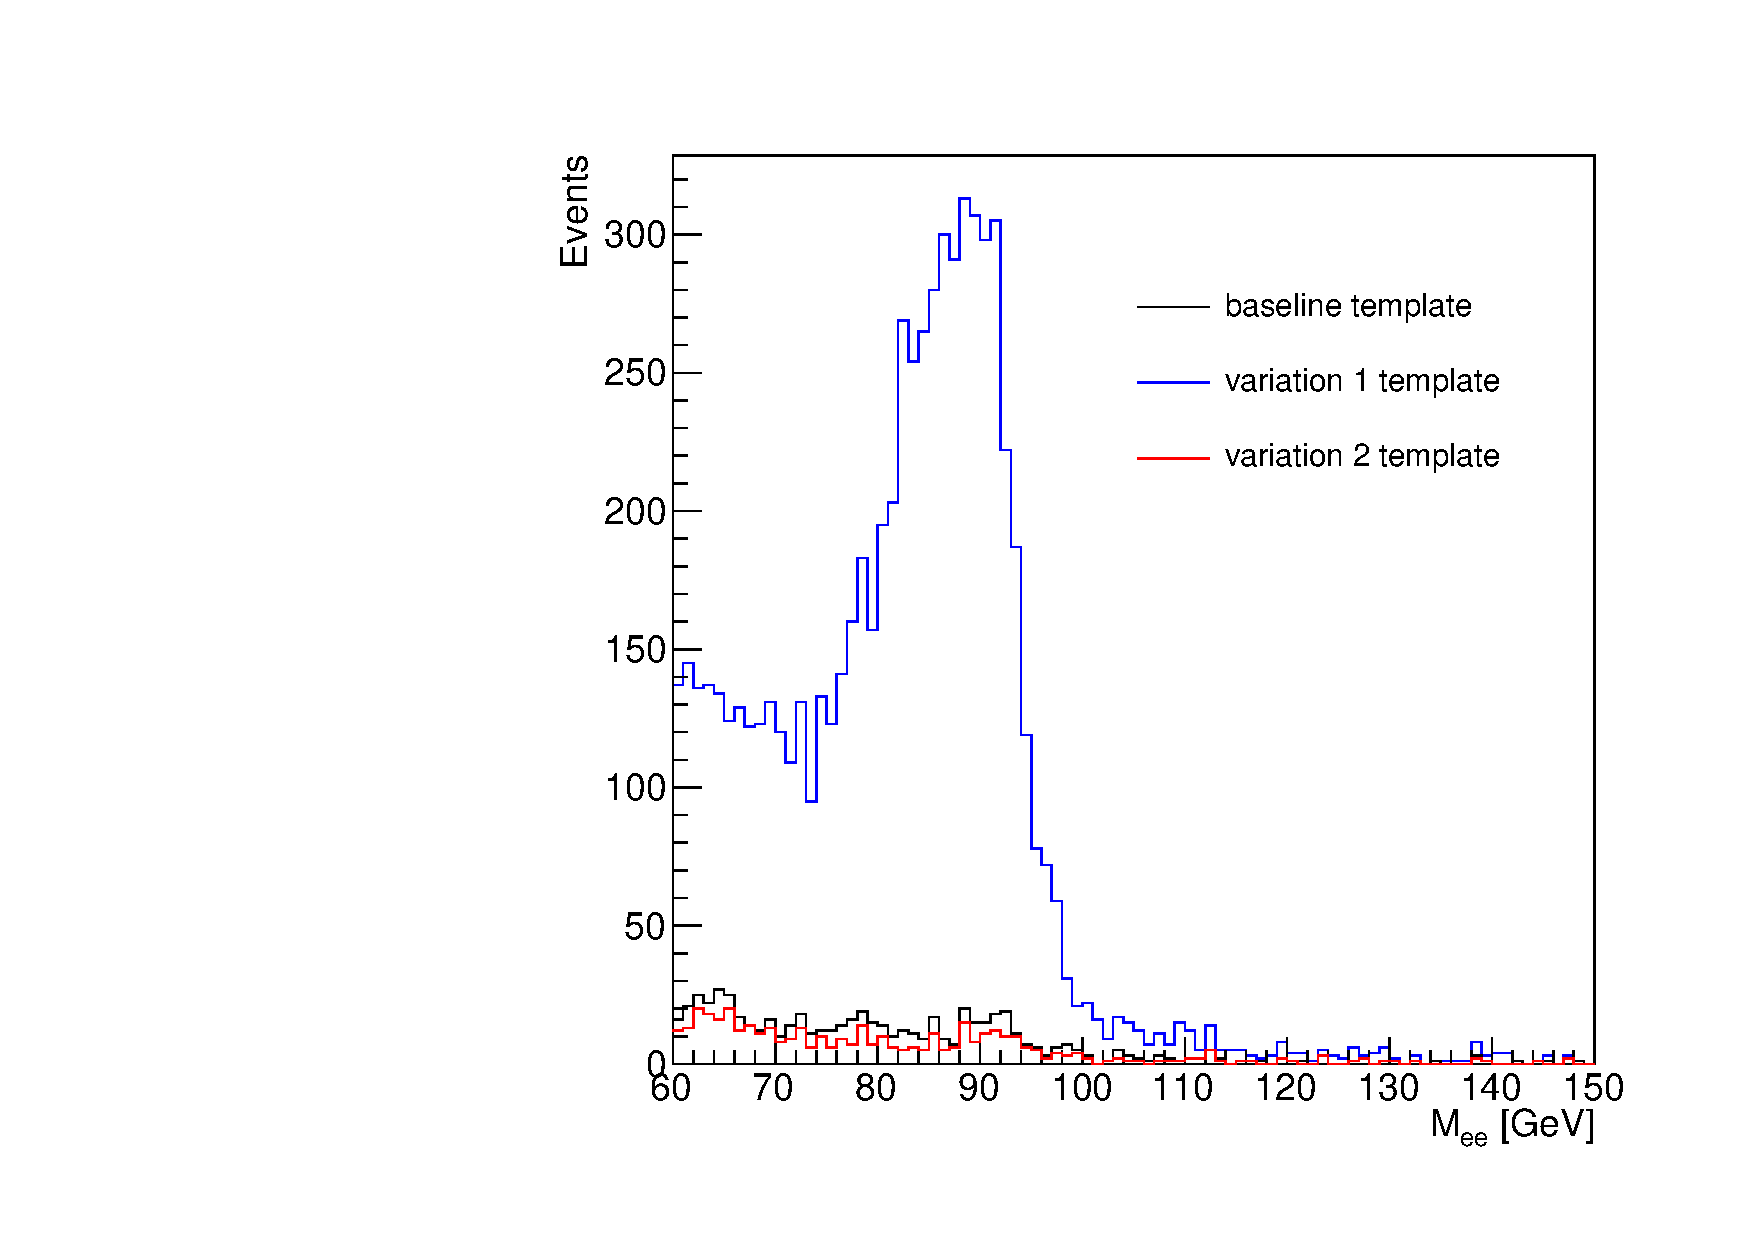
\includegraphics[width=0.48\textwidth]{bkg_template_electron_pt_1520_eta0201.pdf}
\caption{The $m_{ee}$ distributions of the three different background templates.
The $m_{ee}$ distributions in the left and right plots are computed using probe electrons with $10<\pt<15 \GeV$ and $15<\pt<20 \GeV$, respectively.
Because the variation 1 template has looser calorimeter and track isolation requirements, we see a peak in the $Z$ mass region.
Compared with the variation 1 template, the candidate and the variation 2 templates have tighter cuts so no peak can be found in the $Z$ mass region.}
\label{fig:RLE_bkg_templates}
\end{figure}

As the template cuts remove background objects, the background template has to be normalized to provide the correct background estimation.
The $120<m_{ee}<150 \GeV$ region is used for this normalization as a smaller prompt electron contribution is expected in this region.
The background in this tail region is estimated by integrating the candidate $m_{ee}$ distribution in the tail region after subtracting the prompt electron contamination which is estimated by integrating the $m_{ee}$ distribution in the tail region using the $Z\to ee$ MC simulation.
Equation~\ref{eq:RLE_bkg_in_the_tail} shows the estimation of the number of background events in the tail region using the candidate electrons.

\begin{equation}
N_{bkg}^{\textrm{tail}} = N_{\textrm{candidate}}^{\textrm{tail}} - N_{\textrm{MC, prompt}}^{\textrm{tail}}
\label{eq:RLE_bkg_in_the_tail}
\end{equation}

The candidate electron selection criteria already provides a relatively pure sample of prompt electrons.
Therefore, the background template suffers from low statistics in the tail region.
To avoid any bias in the normalization factor due to statistical fluctuations, the template is fitted using an exponential function.
The fitting range is $60<m_{ee}^{\textrm{template}}<120 \GeV$.
In order to minimize the prompt lepton contamination arising from $Z\to ee$ events, the $80< m_{ee}^{\textrm{template}}<100 \GeV$ region is excluded.
Because of the low statistics in the tail, the fit is mostly driven by the $60< m_{ee}^{\textrm{template}}<80 \GeV$.
After applying the fit, the template in the tail region, $N_{\textrm{template}}^{\textrm{tail}}$, is normalized to the background in the tail, $N_{bkg}^{\textrm{tail}}$, to get the correct estimated number of background.
Figure~\ref{fig:RLE_bkg_estimations} shows the candidate $m_{ee}$ distributions before and after applying the background subtraction using the background template.
The data after applying the background subtraction is compared to the MC simulations and the background template distribution and their corresponding fit are also shown.
The simulated $m_{ee}$ distribution of $Z\to ee$ MC are normalized to the data after background subtraction using a Gaussian fit in $85<m_{ee}<95 \GeV$ region.
The top and the bottom rows correspond to the $10<\pt<15 \GeV$ and $15<\pt<20 \GeV$, respectively.
The left, middle, and right columns correspond to the $0<|\eta|<0.8$, $0.8<|\eta|<1.37$, and $1.52<|\eta|<2.0$ regions, respectively.
After applying the background subtraction, the data agree with the MC simulation within the statistical uncertainties.

\begin{figure}[htbp]
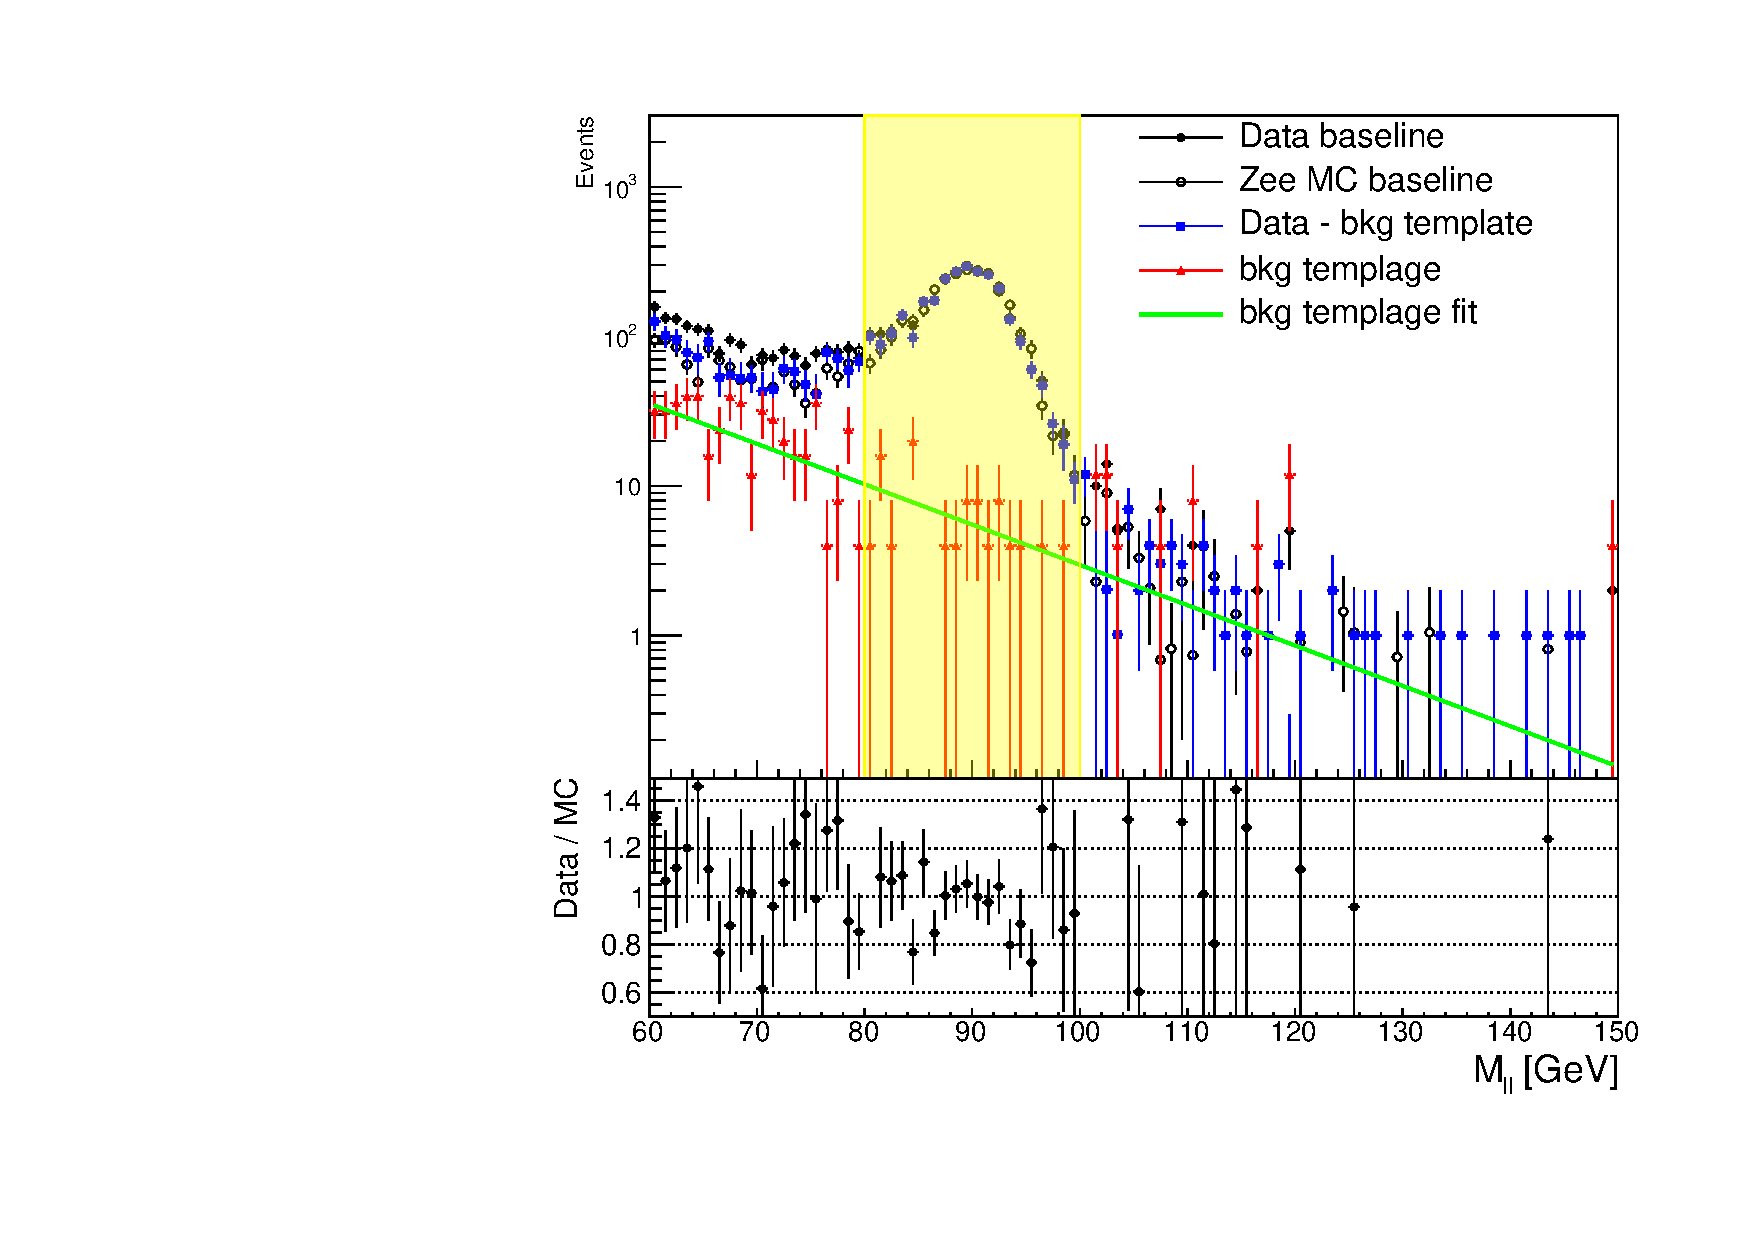
\includegraphics[width=0.33\textwidth]{bkg_subtraction_baseline_template_range_baseline_mll80_100_pt10_15_eta0_80_tag_trigger_matched.pdf}
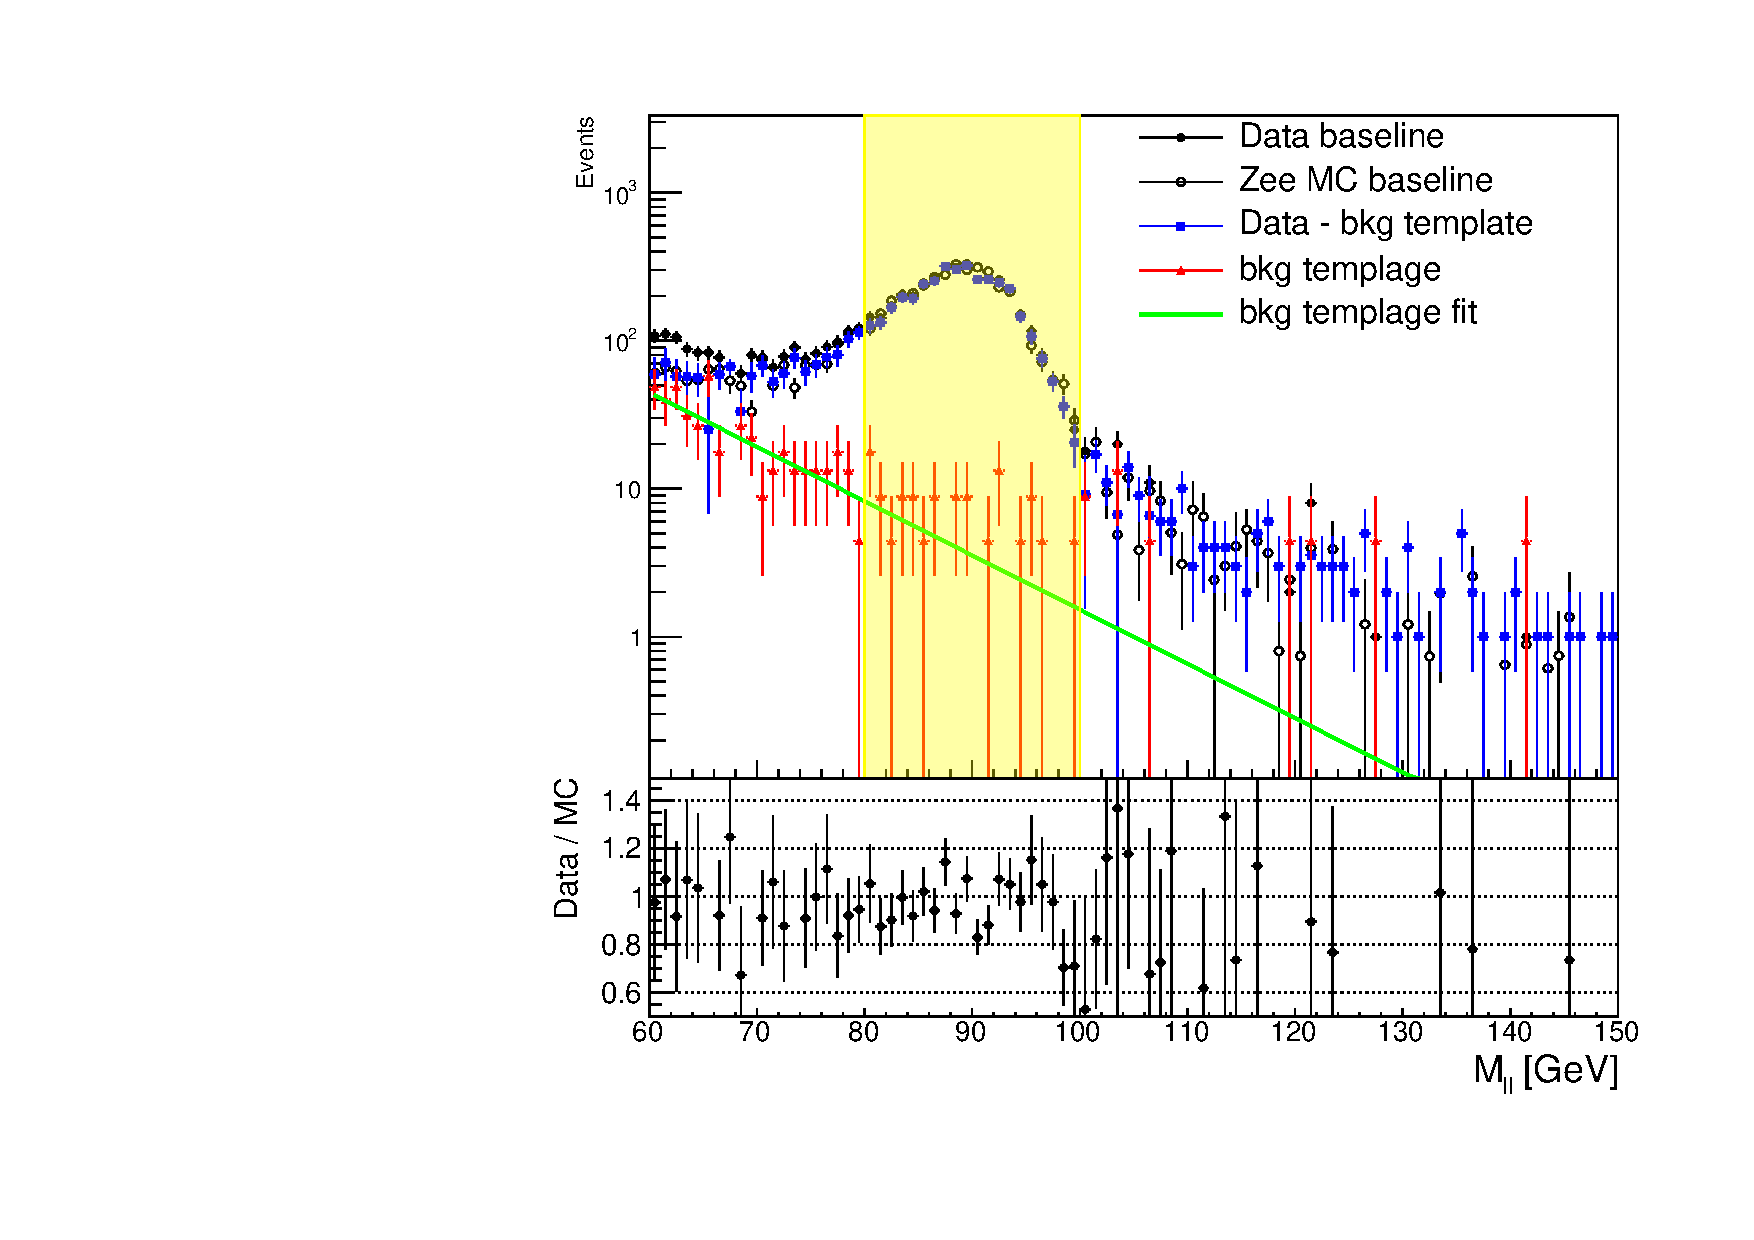
\includegraphics[width=0.33\textwidth]{bkg_subtraction_baseline_template_range_baseline_mll80_100_pt10_15_eta80_137_tag_trigger_matched.pdf}
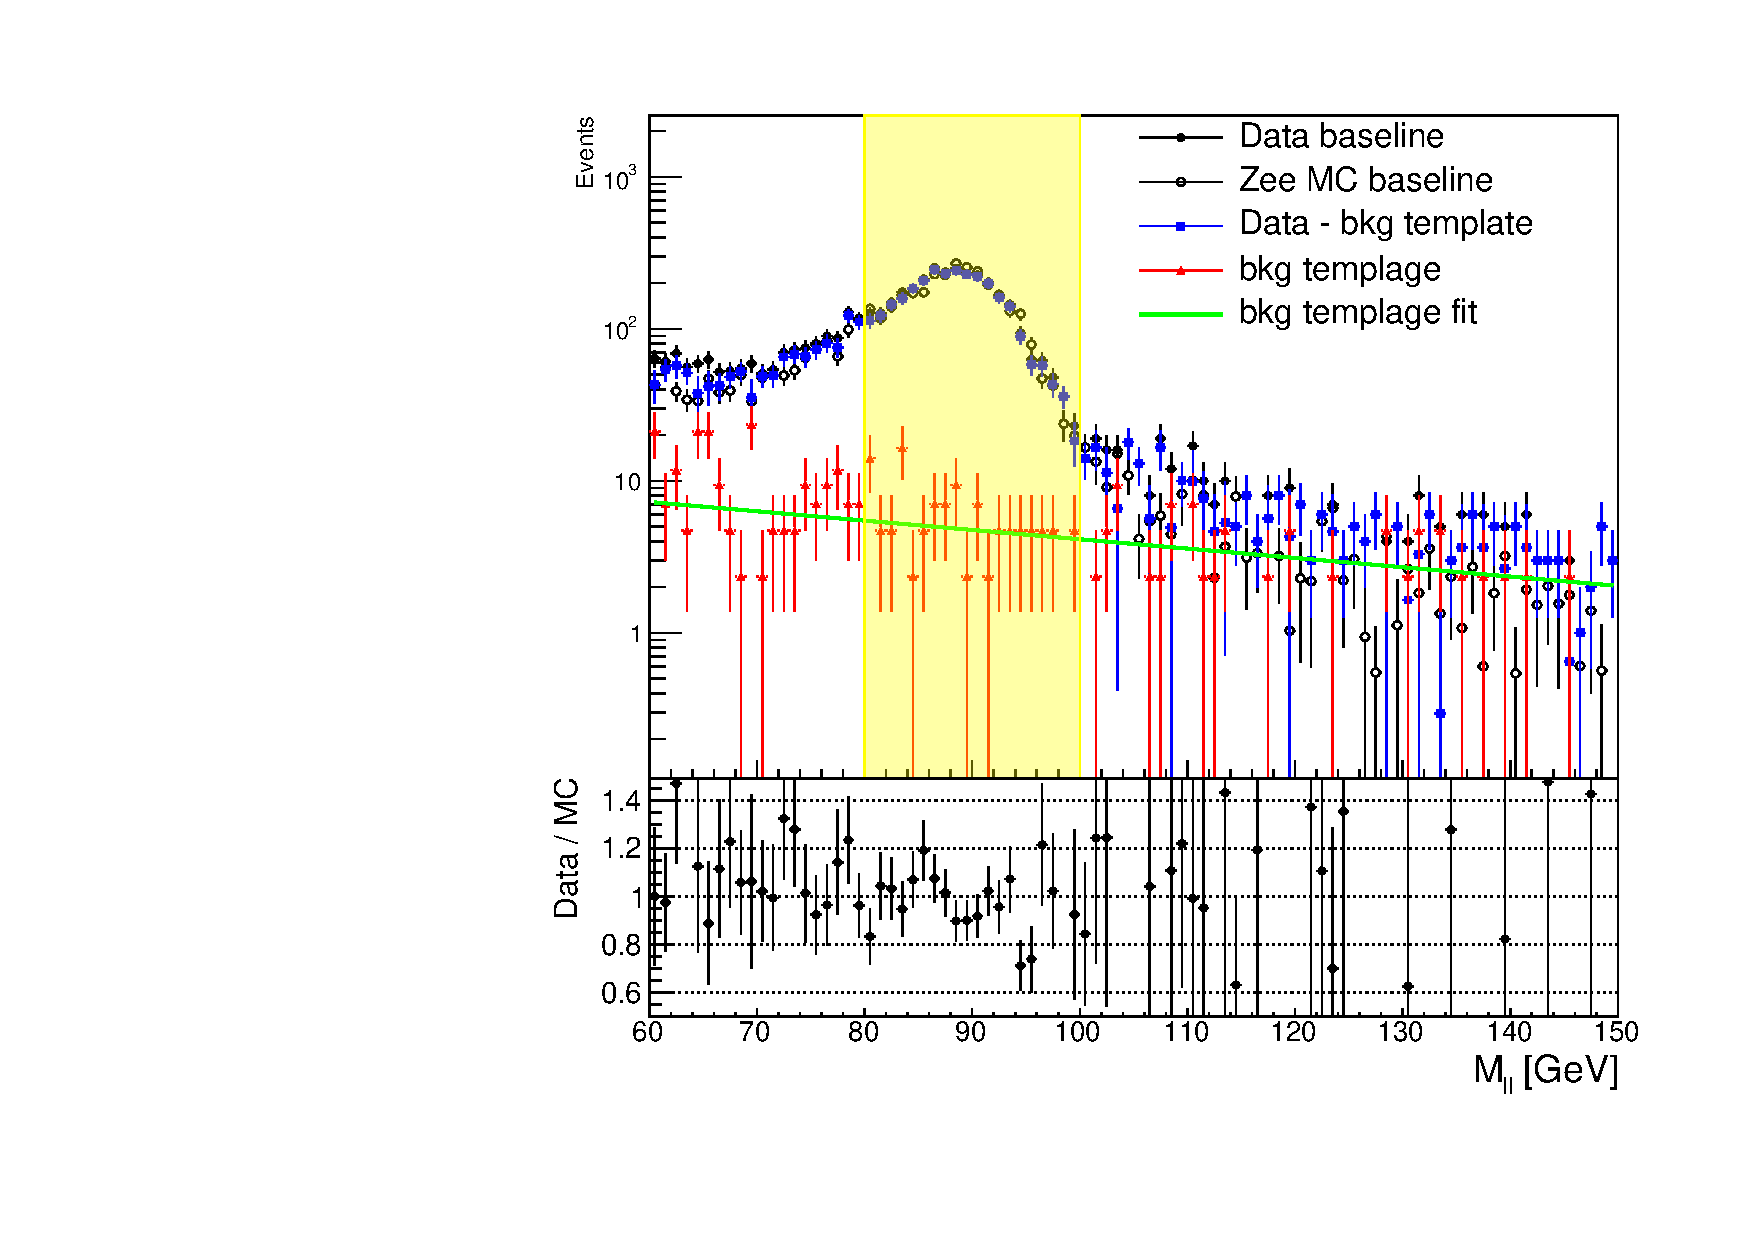
\includegraphics[width=0.33\textwidth]{bkg_subtraction_baseline_template_range_baseline_mll80_100_pt10_15_eta151_200_tag_trigger_matched.pdf}\\
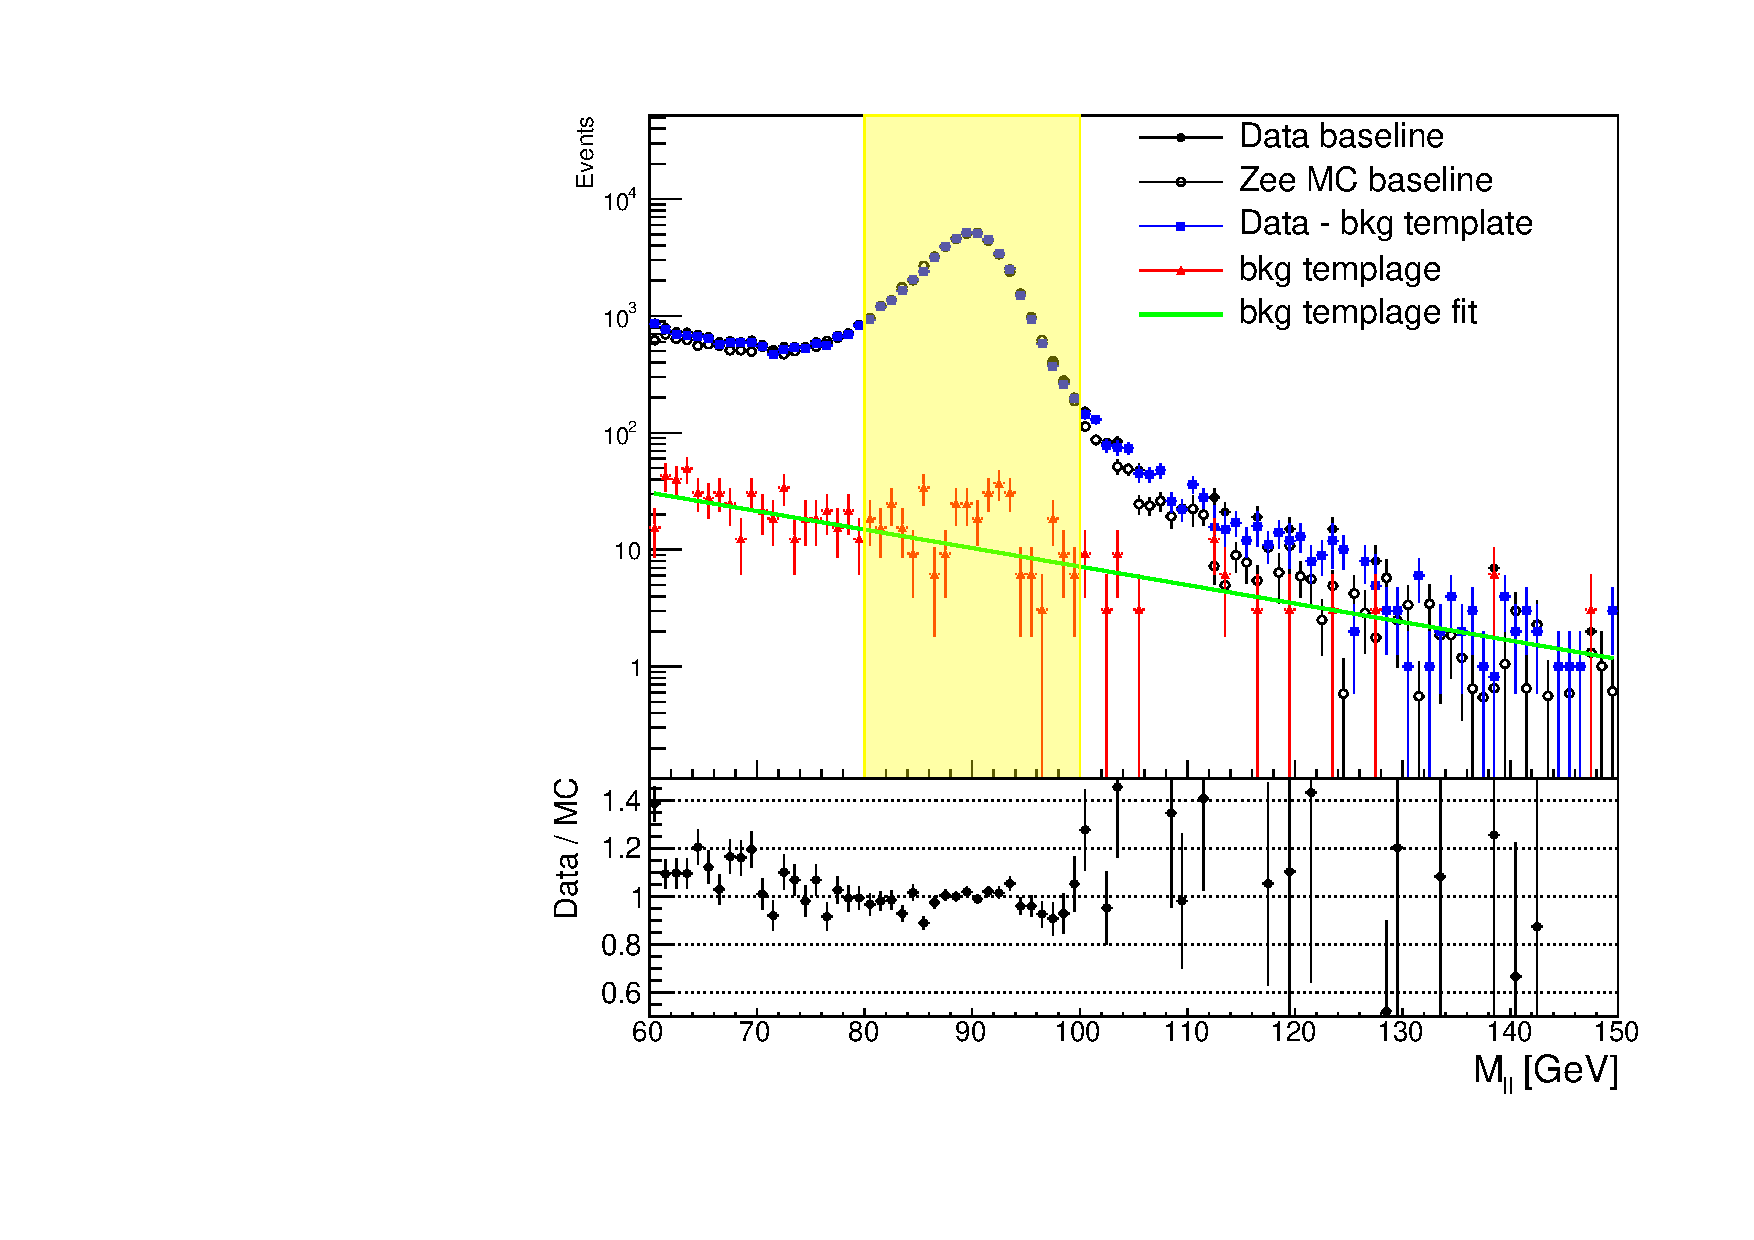
\includegraphics[width=0.33\textwidth]{bkg_subtraction_baseline_template_range_baseline_mll80_100_pt15_20_eta0_80_tag_trigger_matched.pdf}
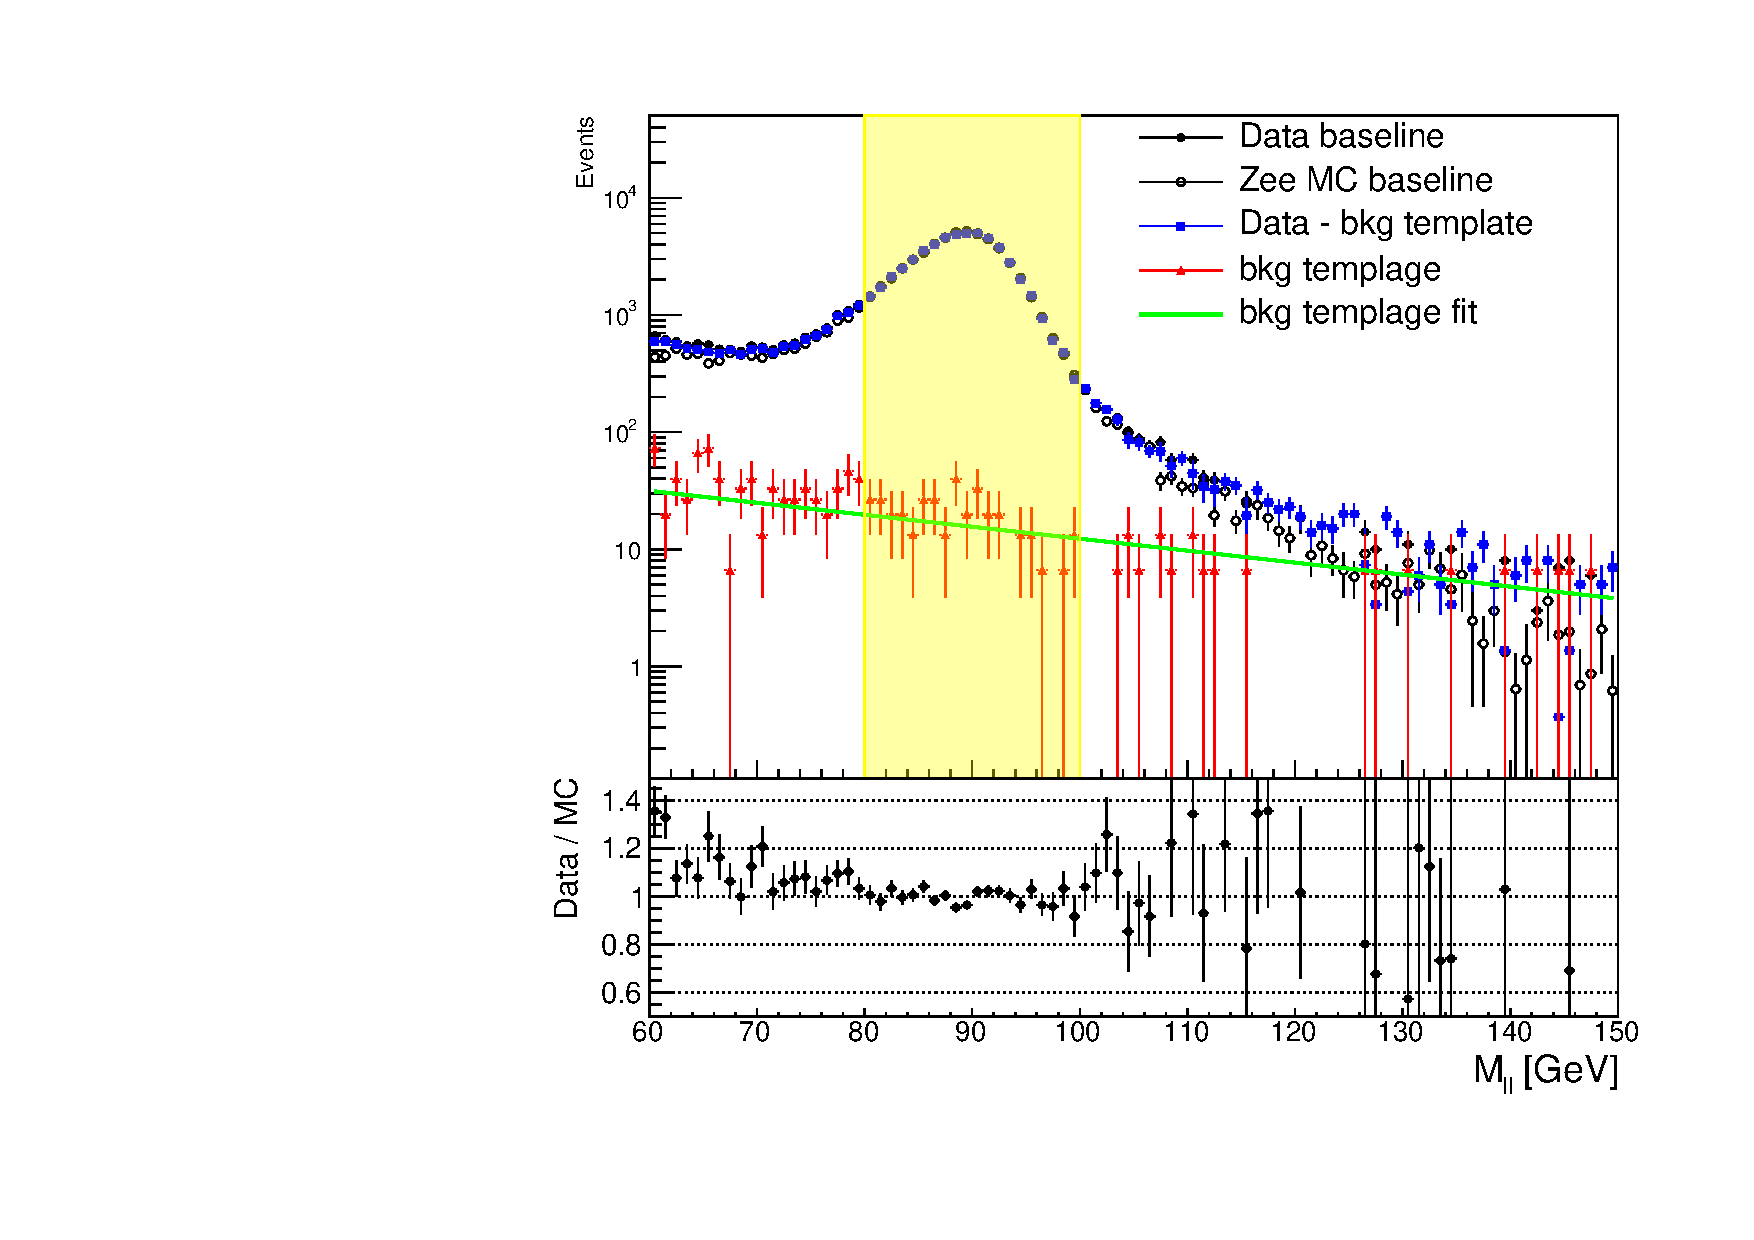
\includegraphics[width=0.33\textwidth]{bkg_subtraction_baseline_template_range_baseline_mll80_100_pt15_20_eta80_137_tag_trigger_matched.pdf}
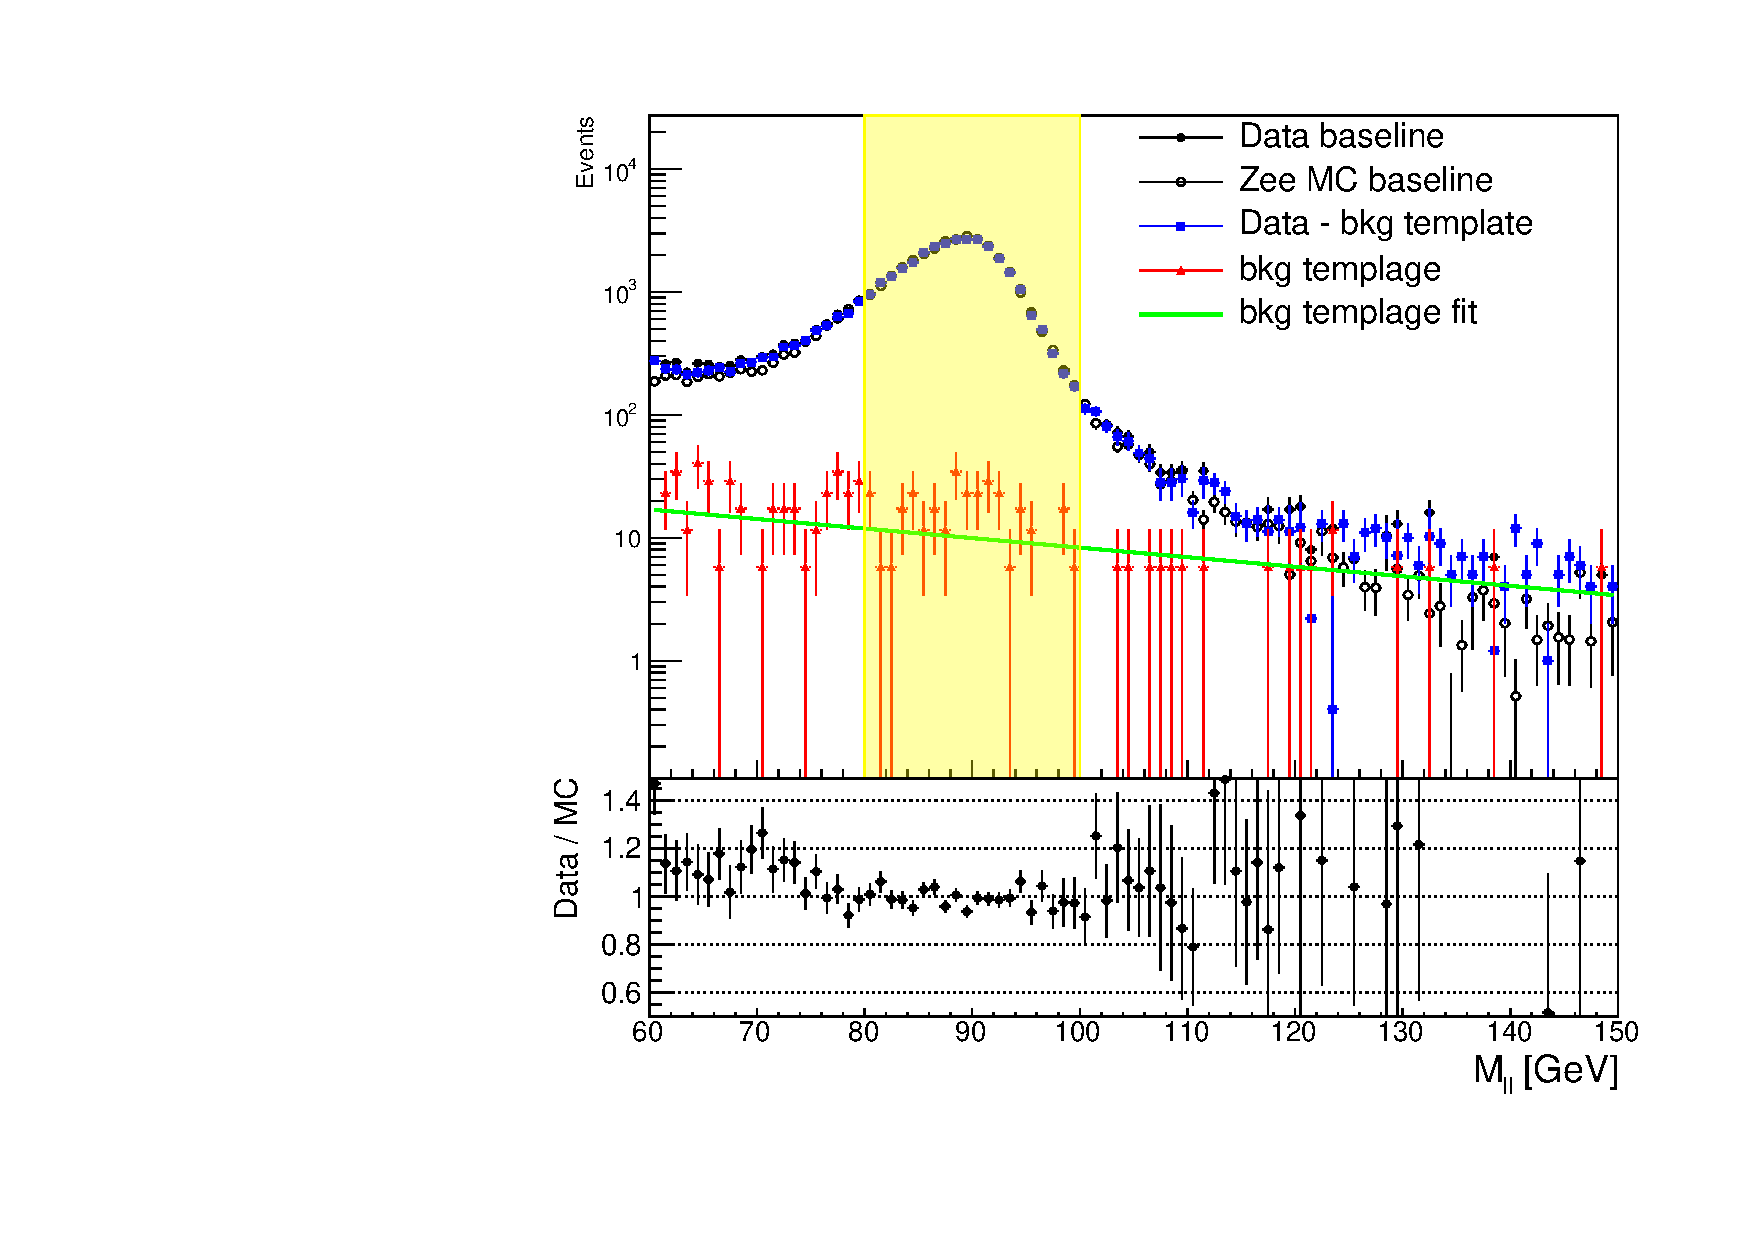
\includegraphics[width=0.33\textwidth]{bkg_subtraction_baseline_template_range_baseline_mll80_100_pt15_20_eta151_200_tag_trigger_matched.pdf}
\caption{Plots illustrate the background subtraction procedure.
The top row represents the $10<\pt<15 \GeV$ region and the the bottom row shows the $15<\pt<20 \GeV$ region.
The three columns, from left to right, are the $0<|\eta|<0.8$, $0.8<|\eta|<1.37$, and $1.52<|\eta|<2.0$ regions, respectively.
The $m_{ee}$ distributions for data before the background subtraction (full black dots) and after the background subtraction (blue squares) are shown along with the corresponding $Z\to ee$ MC distributions (open black circles).
The MC distribution is normalized to the data after the background subtraction using a Gaussian fit of the $Z$ peak region ($85<m_{ee}<95 \GeV$).
The lower panels are the ratio between data after the background subtraction and the MC.
The corresponding background templates (red triangles) and their respective fitting results (green lines) are also shown.
}
\label{fig:RLE_bkg_estimations}
\end{figure}

Then, the background contamination in the $Z$ mass region ($80<m_{ee}<100 \GeV$) is calculated using:

\begin{equation}
N_{bkg}^{80<m_{ee}<100 \GeV} = \int_{80}^{100} N_{\textrm{template}} \ dm_{ee} \cdot \frac{N_{bkg}^{\textrm{tail}}}{N_{\textrm{template}}^{\textrm{tail}}}
\label{eq:RLE_bkg_in_80_mll_100}
\end{equation}

The background estimations are summarized in Table~\ref{tab:RLE_bkg_estimations}.
The largest improvements are observed in the $10<\pt<15 \GeV$ range which a sizeable background contamination is subtracted.
The background contamination in $15<\pt<20 \GeV$ is relatively small and indicates the $Z$ tag-and-probe method provides high purity sample of prompt leptons.
The real electron efficiencies before and after applying the background subtraction are shown in Table~\ref{tab:RLE_efficiency_before_and_after_background_subtraction}.

\begin{table}[htbp]
\begin{center}
\begin{tabular}{cccc}
\hline
\hline
& $0<|\eta|<0.8$ & $0.8<|\eta|<1.37$ & $1.52<|\eta|<2.0$\\
\hline
$10<\pt<15 \GeV$ & 4.04\% & 2.10\% & 3.17\%\\
$15<\pt<20 \GeV$ & 0.44\% & 0.58\% & 0.76\%\\
\hline
\hline
\end{tabular}
\end{center}
\caption{The estimated background contamination using the background template.
The $\pt$ and $|\eta|$ binnings correspond to the one used for the final measurements.}
\label{tab:RLE_bkg_estimations}
\end{table}

\begin{table}[htbp]
\begin{center}
\begin{tabular}{ccccc}
\hline
\hline
& background subtraction & $0<|\eta|<0.8$ & $0.8<|\eta|<1.37$ & $1.52<|\eta|<2.0$\\
\hline
\multirow{2}{*}{$10<\pt<15 \GeV$} & before & $57.4 \pm 0.9$ & $66.6 \pm 0.8$ & $53.2 \pm 0.9$\\
& after & $59.9 \pm 1.9$ & $68.0 \pm 1.8$ & $55.0 \pm 1.7$\\
\hline
\multirow{2}{*}{$15<\pt<20 \GeV$} & before & $64.5 \pm 0.2$ & $69.4 \pm 0.2$ & $62.0 \pm 0.3$\\
& after & $64.8 \pm 0.5$ & $69.8 \pm 0.5$ & $62.5 \pm 0.6$\\
\hline
\hline
\end{tabular}
\end{center}
\caption{The real electron efficiencies in percentage before and after applying the background subtraction.
The efficiency in three different $|\eta|$ regions for $10<\pt<15 \GeV$ and $15<\pt<20 \GeV$ are shown.}
\label{tab:RLE_efficiency_before_and_after_background_subtraction}
\end{table}





%%%
\subsection{Real lepton efficiencies}
\label{subsubsec:RLE_electron_efficiency}

\subsection{>Cut efficiencies}
\label{subsubsec:RLE_cut_efficiencies}

The real lepton efficiency is defined as the ratio between the number of prompt leptons passing the signal lepton definitions and the number of prompt leptons passing the candidate lepton definitions (as defined in~\cite{SS3L-Moriond2017}). Thus, it measures the efficiency of the signal lepton definition cuts with respect to the candidate ones.
The efficiencies associated to each signal cut with respect to candidate definitions are shown in Figure~\ref{fig:RLE_cut_efficiencies}.

\begin{figure}[htbp]
\begin{center}
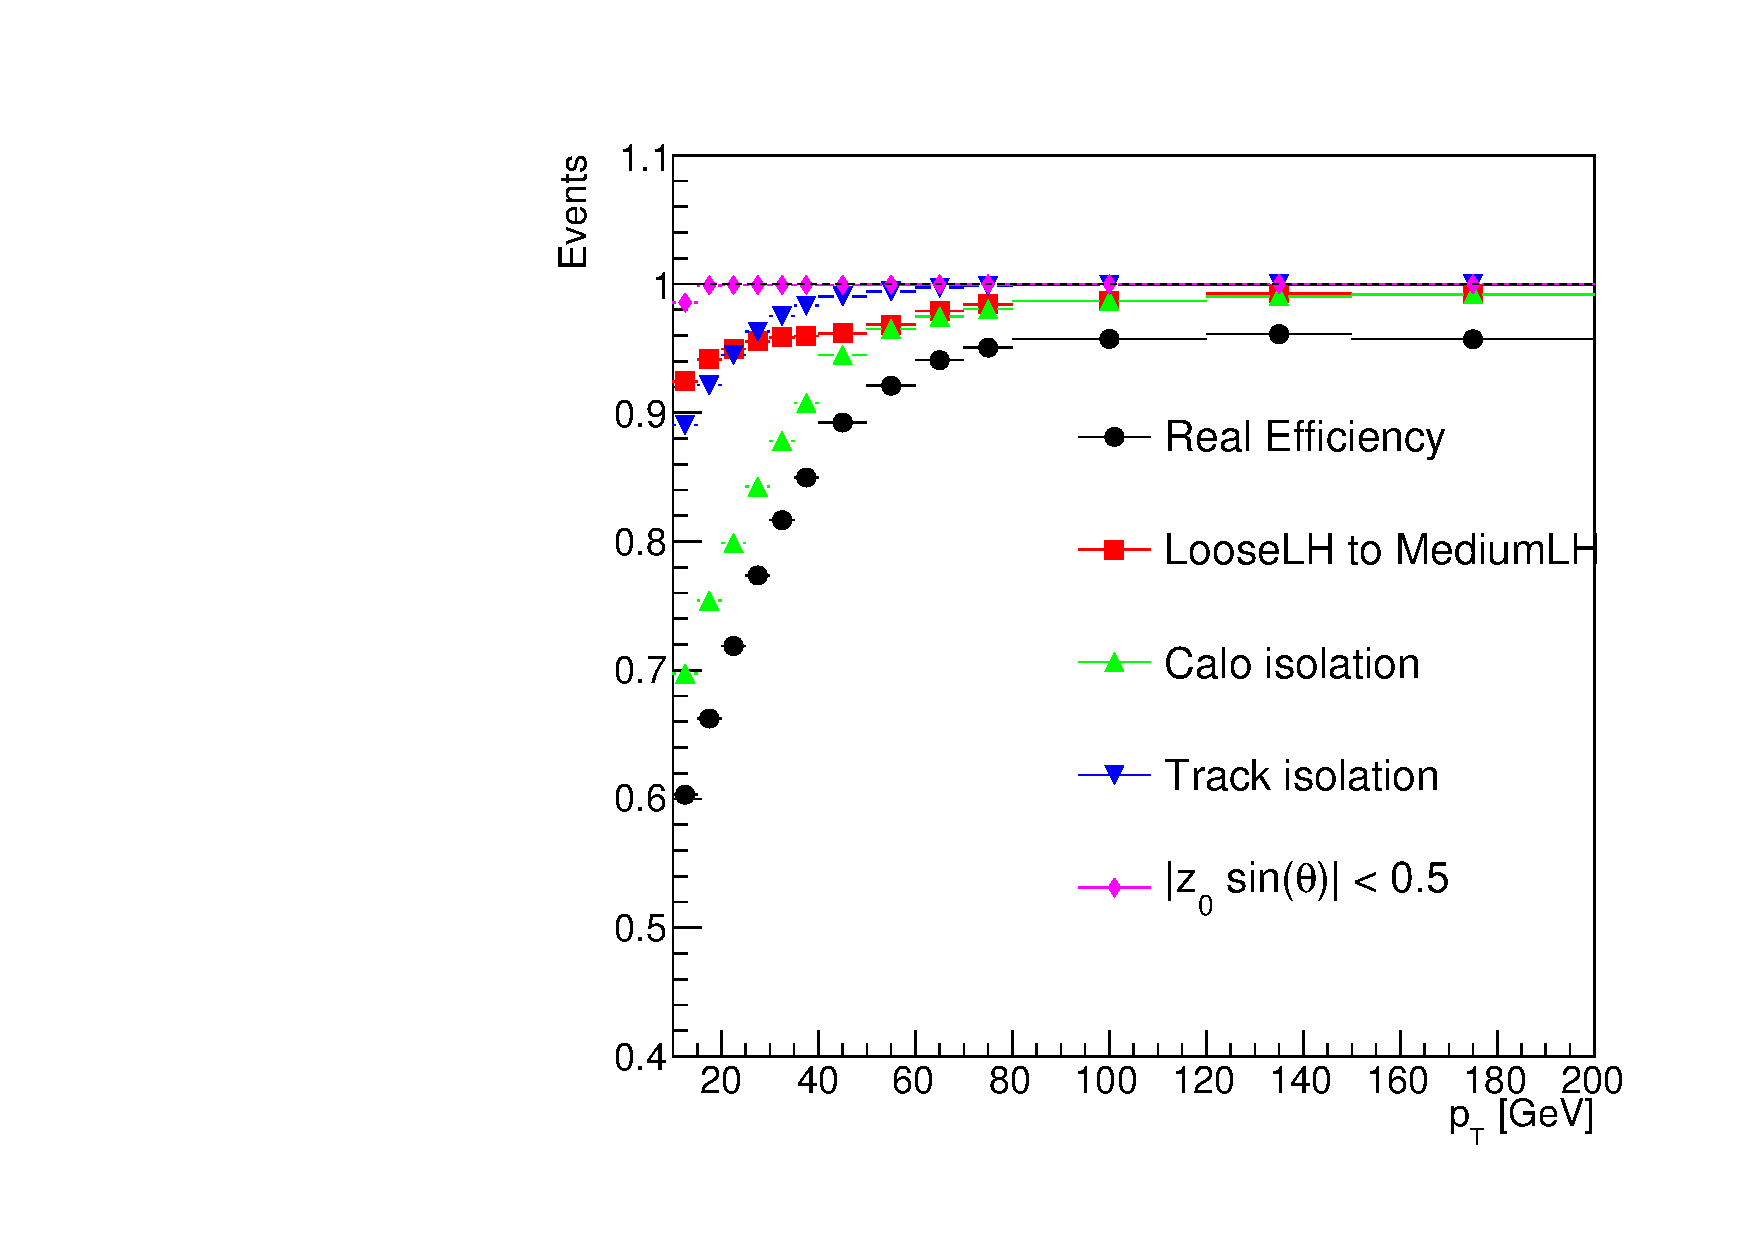
\includegraphics[width=0.48\textwidth]{cut_efficiency_electron}
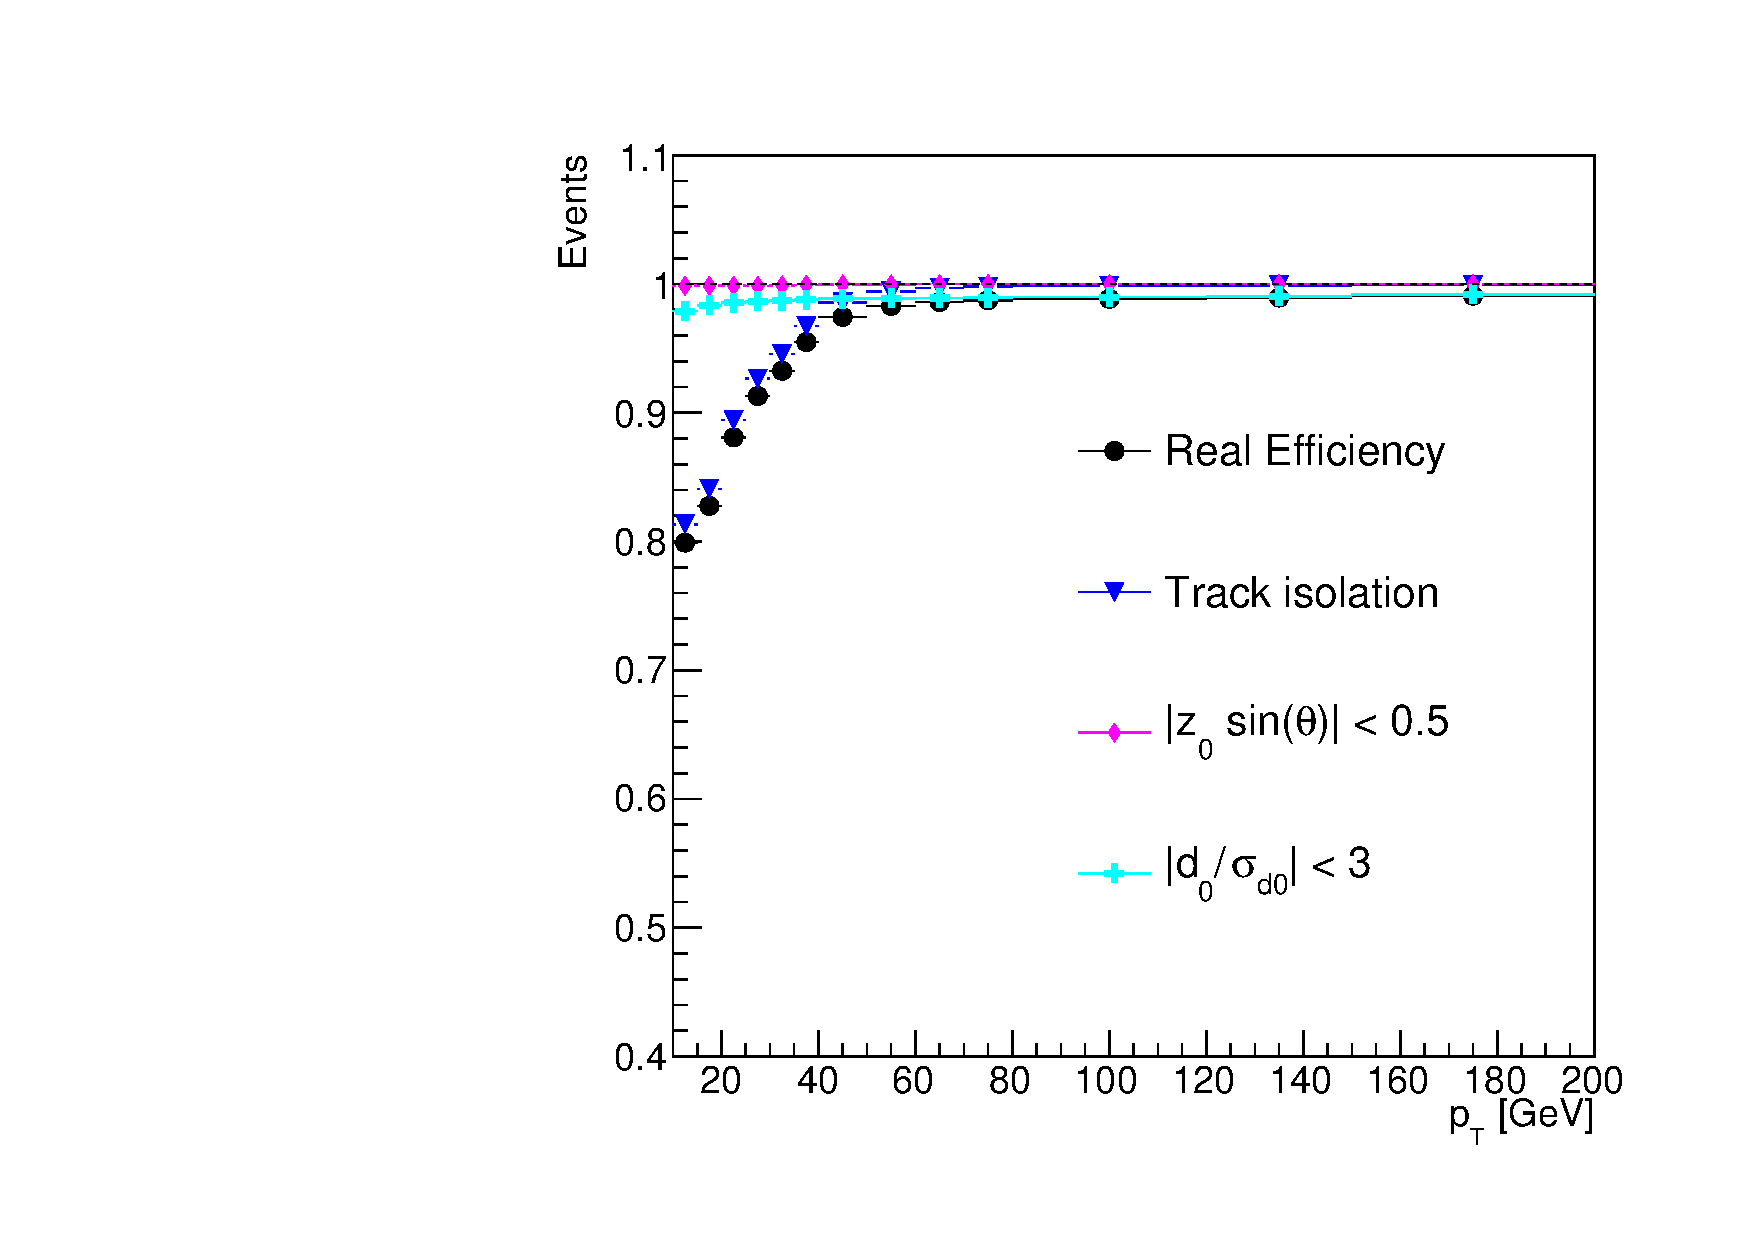
\includegraphics[width=0.48\textwidth]{cut_efficiency_muon}
\caption{Efficiencies of the signal electron (left) and muon (right) definition cuts as a function of $\pt$.
The leptons are selected from data samples using $Z$ tag-and-probe method. The black points correspond to the total real lepton efficiency.
The red squares represent the loose to medium likelihood cut efficiency. The green triangles stand for the calorimeter isolation cut efficiency and the blue triangles are the distribution of track isolation cut efficiency.
The longitudinal and tranverse impact parameters cut efficiencies are presented by magenta diamonds and cyan crosses, respectively.
}
\label{fig:RLE_cut_efficiencies}
\end{center}
\end{figure}

The left plot in Figure~\ref{fig:RLE_cut_efficiencies} shows that the prompt electron efficiency increases from $\sim$62\% in the $10<\pt<15 \GeV$ region to $\sim$98\% when $\pt>80 \GeV$.
The dominant contribution to the electron efficiency losses is the calorimeter isolation.
The loose to medium likelilihood (LH) cut efficiency increases from $\sim$92\% to $\sim$96\% in the $10<\pt<30 \GeV$ region then reaches a plateau for $30<\pt<50 \GeV$ and increases again to $\sim$98\% when $\pt>60 \GeV$.
The calorimeter isolation cut efficiency increases from $\sim$ 69\% in the $10<\pt<15 \GeV$ region to $\sim$98\% when $\pt>70 \GeV$.
The efficiency associated to the track isolation cut is $\sim$89\% for $10<\pt<15 \GeV$ and increases up to $\sim$100\% when $\pt>60 \GeV$.
The contribution of the longitudinal impact parameter cut to the real efficiency is $\sim$98\% for $10<\pt<15 \GeV$ and increases up to $\sim$100\% when $\pt>15 \GeV$.

As the same muon identification is used for the candidate and the signal definitions, the muon efficiencies are much higher than the electron ones (Figure~\ref{fig:RLE_cut_efficiencies}, right hand side).
The associated efficiencies computed using $Z\to \mu \mu$ events increase from $\sim$80\% for $10<\pt<15 \GeV$ to $\sim$98\% when $\pt>50 \GeV$.
The dominant contribution to the muon efficiency is the track isolation cut. The associated efficiency increases from $\sim$82\% to 98\% when $\pt>50 \GeV$.
Another difference with the electron case is that a transverse impact parameter cut is used in the muon signal definitions while this cut is already applied at the candidate level in the electron case.
The contributions of the longitudinal and transverse impact parameter cuts on muon efficiency are very small because the cut efficiency of transverse impact parameter is $\sim$99\% and the longitudinal one is 100\%.



\subsection{>Real lepton efficiencies}
\label{subsubsec:RLE_results}

Figure~\ref{fig:RLE_real_efficiency_total_systematics} shows the real lepton efficiencies as a function of \pt and $|\eta|$ used by the matrix method.
The three $|\eta|$ binnings used for the electron case are driven by the electromagnetic calorimeter geometry.
The background subtraction has been applied on the $10<\pt<15 \GeV$ and $15<\pt<20 \GeV$ for the electron case.
Because the crack region, $1.37<|\eta|<1.52$, is not considered in the analysis, this region is removed from the real electron efficiency study.
The uncertainties are the quadratic sum of the statistical uncertainties and the measurement systematic uncertainties.
The electron efficiencies in $1.52<|\eta|<2.01$ are lower than the other two $|\eta|$ regions.
This is expected as the electron identification is better in the central region of the calorimeter. 

\begin{figure}[htbp]
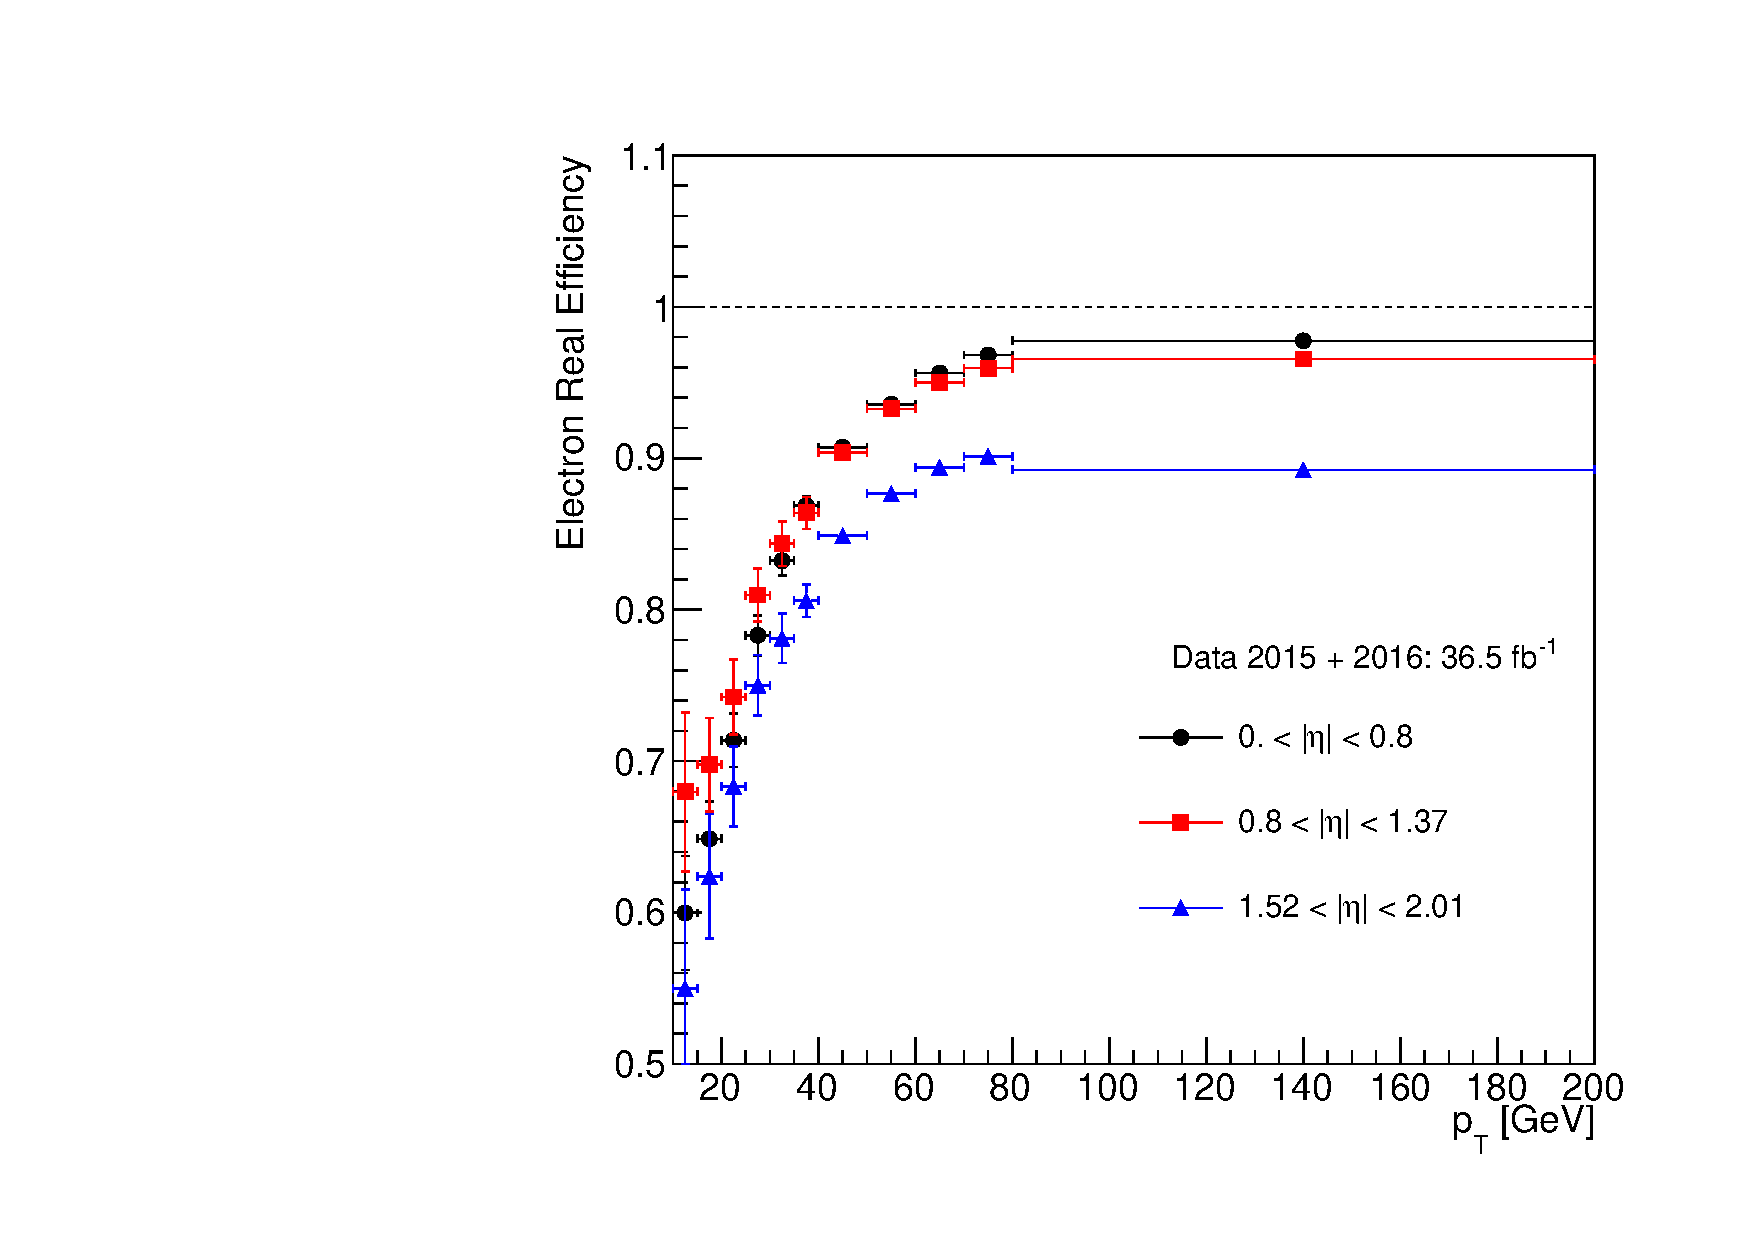
\includegraphics[width=0.48\textwidth]{real_electron_efficiency_total_systematics.pdf}
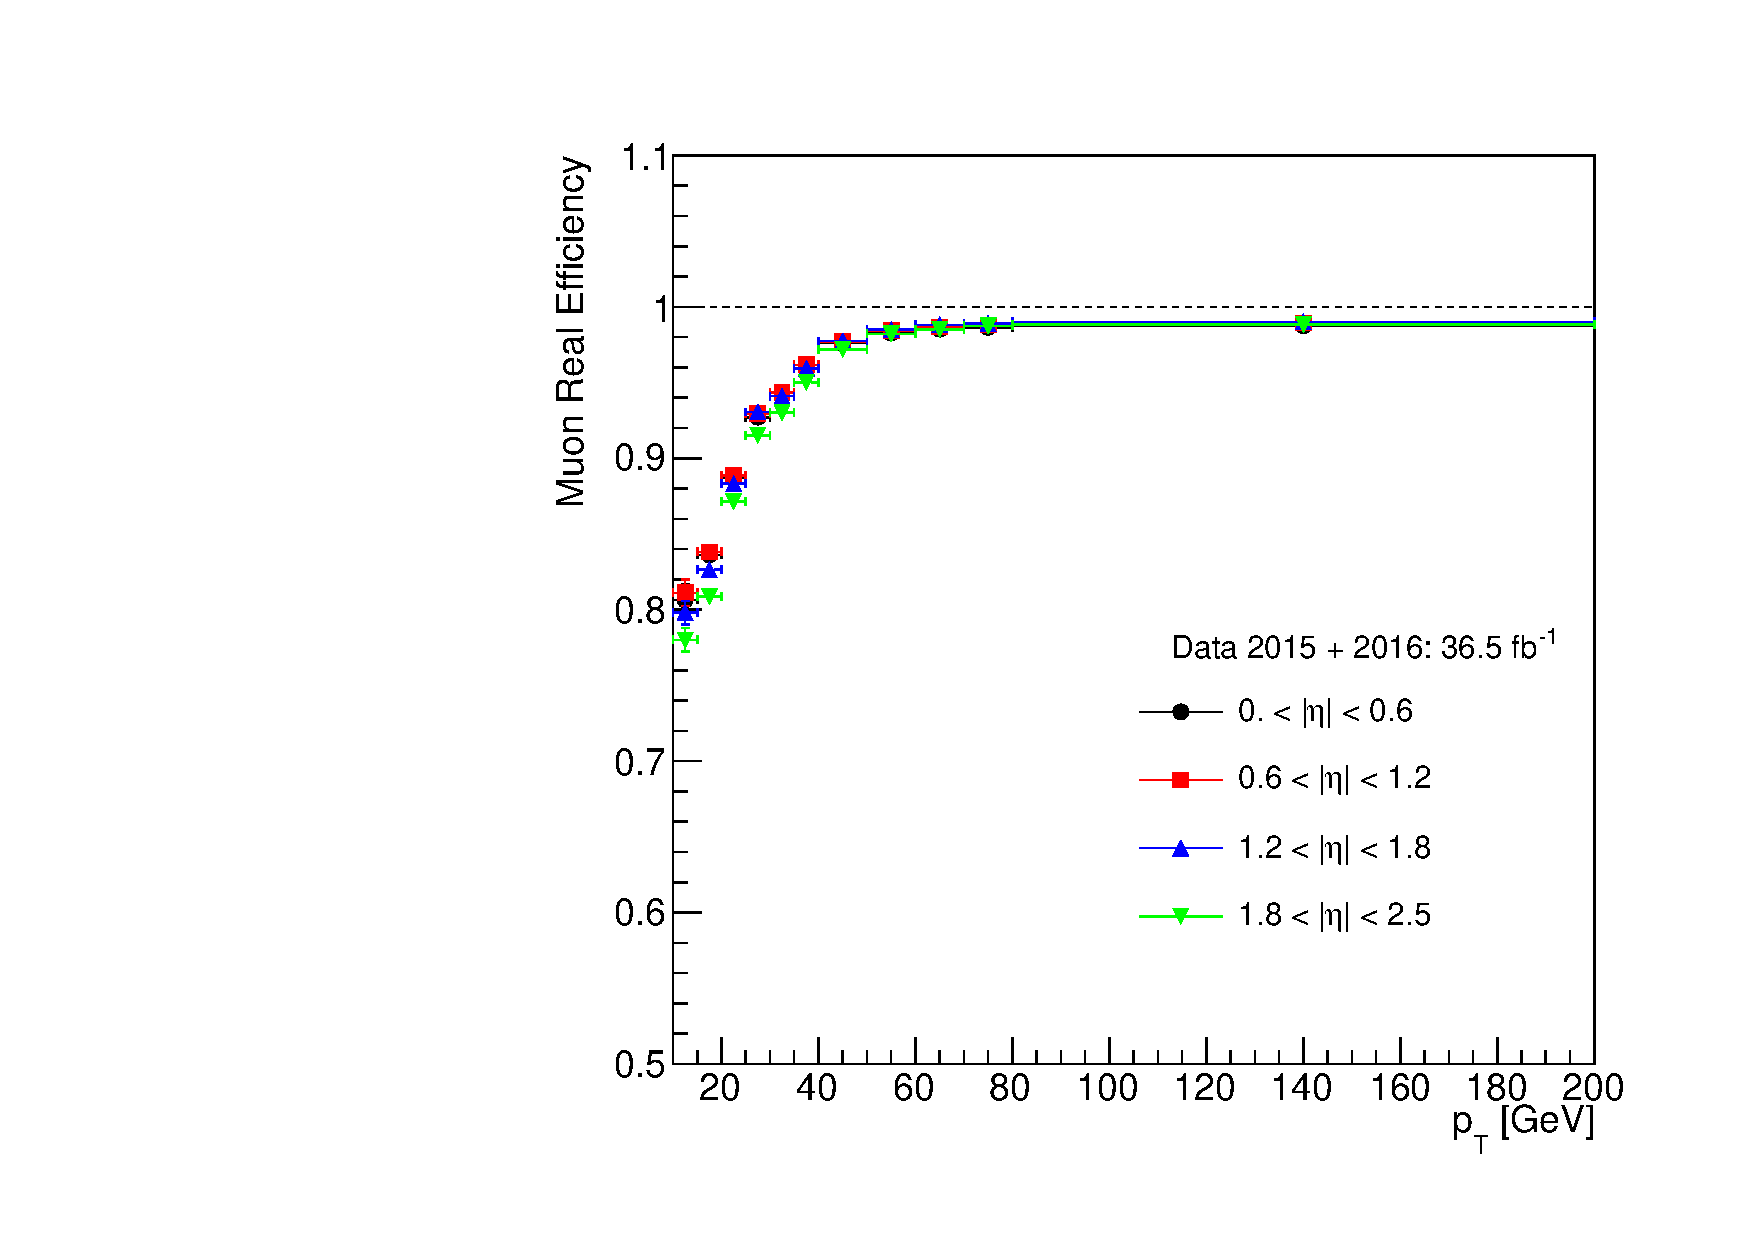
\includegraphics[width=0.48\textwidth]{real_muon_efficiency_total_systematics.pdf}
\caption{The real lepton efficiencies as a function of \pt and $|\eta|$ measured using the $Z$ tag-and-probe method.
The left plot corresponds to the real electron efficiencies in three $|\eta|$ regions and the right plot stands for the real muon efficiencies in four $|\eta|$ regions.
The $|\eta|$ binning used for the real electron efficiencies measurement corresponds to the geometry of the electromagnetic calorimeter and removing the creak region.
A homogeneous $|\eta|$ binning has been chosen for the muon case.}
\label{fig:RLE_real_efficiency_total_systematics}
\end{figure}



\subsection{>Tag-and-probe method and truth matching comparisons}
\label{subsubsec:RLE_truth_matched}

Although the $Z$ tag-and-probe method could select probe leptons accuratly, we would like to verify the accuracy of the $Z$ tag-and-probe method by comparing it with the truth matched information using the $Z\to\ell\ell$ MC samples.
Figure~\ref{fig:RLE_TandP_truth_match_comparisons} shows the real lepton efficiencies computed using $Z$ tag-and-probe method and truth matching as a function of $\pt$, $|\eta|$, and $\Delta R(\ell, jet)$, respectively.
The uncertainties shown in the plots correspond to the statistical uncertainties only.
There are as large as 7\% differences in the low $\pt$ region for the real electron efficiencies as function of $\pt$ computed by these two different methods.
The differences decrease when $\pt$ increases and no differences can be seen when $\pt>50 \GeV$.
The largest differences is about 3\% in the real electron efficiencies as a function of $|\eta|$.
Larger differences between these two methods can be seen in the real electron efficiencies as a function of $\Delta R(e, jet)$ when the $\Delta R(e, jet)<0.4$ because the overlap removal requirement has been applied on the candidate electrons.
The overlap removal removes the electrons so the $\Delta R(e, jet)<0.4$ region lacks statistics.
The efficiency differences between $Z$ tag-and-probe method and truth matching are less then 1\% for the muon case except the real muon efficiencies as a function of $\Delta R(\mu, jet)$ which has larger differences between these two methods when $\Delta R(\mu, jet)<0.4$ also because of the overlap removal requirement.
The comparisons showing small differences between methods indicate the probe leptons selected by the $Z$ tag-and-probe method are reliable and the differences may be considered as the systematic uncertainties.

\begin{figure}[htbp]
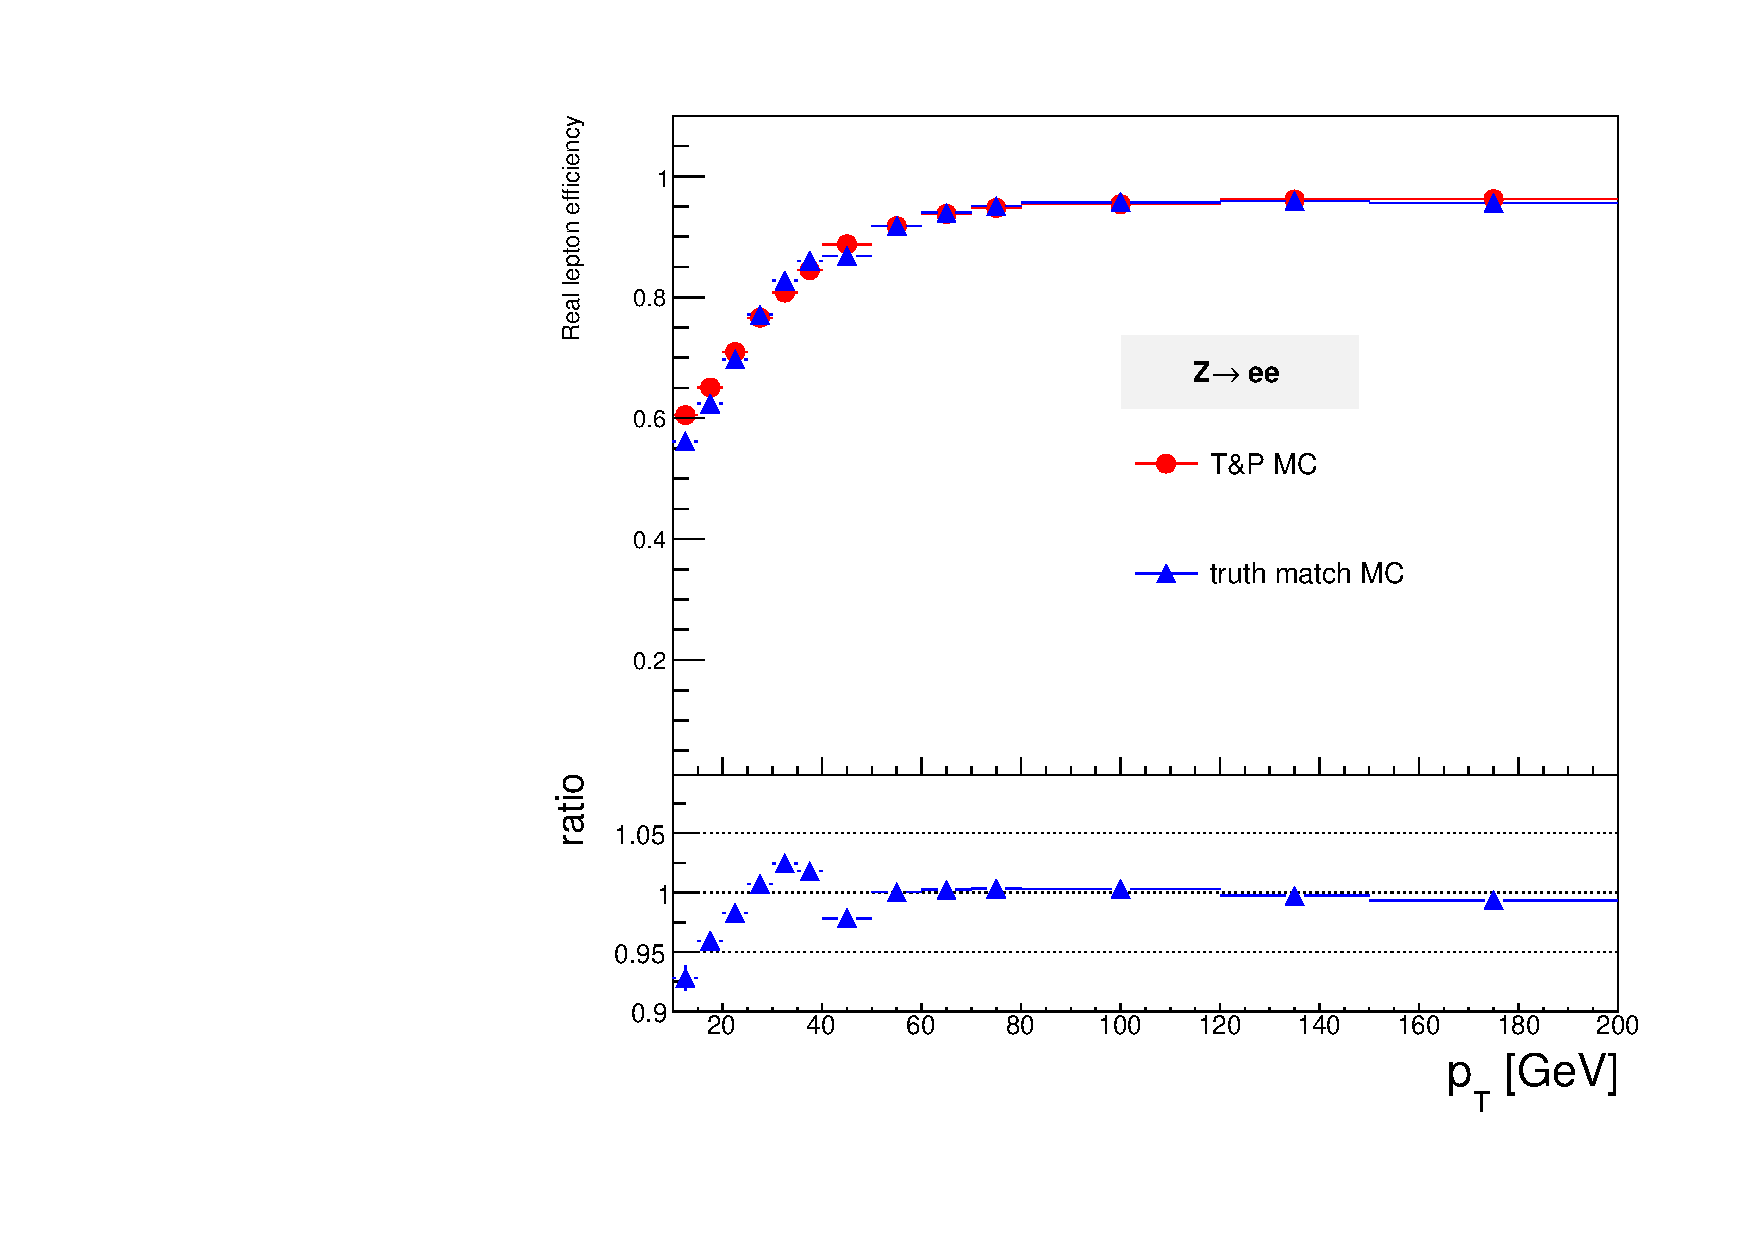
\includegraphics[width=0.33\textwidth]{Compare_TandP_truth_match_electron_pt.pdf}
\includegraphics[width=0.33\textwidth]{Compare_TandP_truth_match_electron_eta.pdf}
\includegraphics[width=0.33\textwidth]{Compare_TandP_truth_match_electron_dRjet.pdf}\\
\includegraphics[width=0.33\textwidth]{Compare_TandP_truth_match_muon_pt.pdf}
\includegraphics[width=0.33\textwidth]{Compare_TandP_truth_match_muon_eta.pdf}
\includegraphics[width=0.33\textwidth]{Compare_TandP_truth_match_muon_dRjet.pdf}
\caption{
The real lepton efficiencies computed using $Z$ tag-and-probe method and truth matching.
The top row is the electron case and the bottom row is the muon case.
The three columns from the left to the right are the real lepton efficiencies as a function $\pt$, $|\eta|$, and $\Delta R(\ell, jet)$, respectively.
The real lepton efficiencies computed using $Z$ tag-and-probe are denoted by the red dots and the one calculated using truth matching are indicated by the blue triangles.
The lower pads show the ratio with respect to the $Z$ tag-and-probe method.
}
\label{fig:RLE_TandP_truth_match_comparisons}
\end{figure}



\subsection{>Data-to-MC comparisons}
\label{subsubsec:RLE_data_to_mc_comparisons}

The real lepton efficiencies computed using the $Z$ tag-and-probe method in data are compared to those using the simulated $Z\to \ell\ell$ MC processes.
All 2015 and 2016 data are considered, and corresponds to an integrated luminosity of 36.5 fb$^{-1}$ after good run list requirements.
All the MC lepton scale factors provided by the CP group are applied and the simulation is reweighted to the pile-up observed in the data.
%Besides, an additional truth match is added for the MC lepton selection.
Figure~\ref{fig:RLE_real_efficiency_pt_eta_dRjet} shows the electron and the muon real efficiencies as a function of $\pt$, $|\eta|$ and $\Delta R(\ell, jet)$ measured on data and with simulated $Z\to ee$ and $Z\to \mu\mu$ MC processes, respectively.
The associated uncertainties correspond to the statistical uncertainties only.
A reasonable data to MC agreement is observed except the low $\Delta R(\ell, jet)$ region because of lacking statistics.
The real electron efficiencies as a function of $|\eta|$ computed using the $Z\to ee$ MC are slightly lower than the one computed using data.
The differences come from the efficiencies drop of $Z\to ee$ MC in the $40<\pt<50 \GeV$. 

\begin{figure}[htbp]
%\includegraphics[width=0.96\textwidth]{real_efficiency.pdf}
\includegraphics[width=0.33\textwidth]{real_efficiency_ratio_plot_electron_pt.pdf}
\includegraphics[width=0.33\textwidth]{real_efficiency_ratio_plot_electron_eta.pdf}
\includegraphics[width=0.33\textwidth]{real_efficiency_ratio_plot_electron_dRjet.pdf}\\
\includegraphics[width=0.33\textwidth]{real_efficiency_ratio_plot_muon_pt.pdf}
\includegraphics[width=0.33\textwidth]{real_efficiency_ratio_plot_muon_eta.pdf}
\includegraphics[width=0.33\textwidth]{real_efficiency_ratio_plot_muon_dRjet.pdf}
\caption{The real lepton efficiencies as a function of $\pt$, $|\eta|$ and $\Delta R(\ell, jet)$ measured on data and MC using the $Z$ tag-and-probe method.
The plots on the top row correspond to the real electron efficiencies and the plots on the bottown row correspond to the real muon efficiencies.
The 2015 + 2016 data are denoted by the black dots, the $Z\to\ell\ell$ MC are shown using red squares and are reweighted to the data pile-up.
The uncertainties shown in the plots are corresponding to the statistical uncertainties only.
Some differences between data and $Z\to \ell\ell$ MC can be seen in the low $\Delta R(\ell, jet)$ region.
The binning used for the real electron efficiencies as a function of $\eta$ corresponds to the geometry of the electromagnetic calorimeter.}
\label{fig:RLE_real_efficiency_pt_eta_dRjet}
\end{figure}



\subsection{>Real lepton efficiency versus pileup}
\label{subsubsec:RLE_vs_pileup}
 
The relations between the real lepton efficiencies and the pileup are also studied.
The efficiencies calculated using 2015 + 2016 data are compared with those obtained using $Z$ tag-and-probe method and truth matching MC samples.
The \ttbar and $\tilde{g}\to\ttbar\tilde{\chi^{0}_{1}}$ MC samples are also considered because we are interested in the behavior of the efficiencies with different event topologies.
Figure~\ref{fig:RLE_vs_pileup} shows the electron and muon real efficiencies as a function of the average interactions per crossing $<\mu>$.
The real electron efficiencies are about 92\% to 93\% at low $<\mu>$ and decrease when $<\mu>$ increase.
Comparing with the real lepton efficiencies calculated by data samples, the efficiencies computed using $\tilde{g}\to\ttbar\tilde{\chi^{0}_{1}}$ MC sample have lower efficiencies in both electron and muon cases.
But the real lepton efficiencies computed by the \ttbar have similar efficiencies with the data one in the electron case and have lower efficiencies in the muon case.
This is because the \ttbar MC has lower real muon efficiencies when $\pt<40 \GeV$ with respect to data.
If we require a $\pt>40 \GeV$ requirement on the probe leptons, then the real muon efficiencies for \ttbar MC agree with data.
The electron and muon real efficiencies as a function of $\pt$ compared with data and $Z\to\ell\ell$ are shown in Figure~\ref{fig:RLE_real_efficiency_ttbar_gtt}.
From which we notice the real lepton efficiencies of \ttbar process is lower than the data one when $\pt<40 \GeV$ and the $\tilde{g}\to\ttbar\tilde{\chi^{0}_{1}}$ process has lower real lepton efficiencies in both electron and muon cases.

\begin{figure}[htbp]
\includegraphics[width=0.48\textwidth]{real_efficiency_vs_AvgMu_elec.pdf}
\includegraphics[width=0.48\textwidth]{real_efficiency_vs_AvgMu_muon.pdf}
\caption{
The real lepton efficiencies as a function of the average interactions per crossing $<\mu>$.
The data is shown as black dots and $Z\to \ell\ell$ tag-and-probe and truth matching are in red squares and blue triangles, respectively.
The real lepton efficiencies calculated using \ttbar and $\tilde{g}\to\ttbar\tilde{\chi^{0}_{1}}$ MC are also shown in magenta diamonds and yellow crosses.
And they show the real lepton efficiencies with different event topoloties.
The $|\eta|<2$ requirement has been applied on the \ttbar and $\tilde{g}\to\ttbar\tilde{\chi^{0}_{1}}$ MC samples for the electron case.
}
\label{fig:RLE_vs_pileup}
\end{figure}

\begin{figure}[htbp]
\includegraphics[width=0.48\textwidth]{real_efficiency_ratio_plot_electron_pt_ttbar_gtt.pdf}
\includegraphics[width=0.48\textwidth]{real_efficiency_ratio_plot_muon_pt_ttbar_gtt.pdf}
\caption{
The electron and muon real efficiencies as a function of $\pt$.
The black dots stands for data, the red squares and blue triangles indicate $Z\to\ell\ell$ tag-and-probe and truth matching, respectively.
The \ttbar and $\tilde{g}\to\ttbar\tilde{\chi^{0}_{1}}$ are represented by magenta diamonds and yellow crosses, respectively.
All of the real lepton efficiencies computed by MC processes are agree with the data one when $\pt>40 \GeV$.
The differences in the $\pt<40 \GeV$ region come from the different event topologies. 
}
\label{fig:RLE_real_efficiency_ttbar_gtt}
\end{figure}

%%% 
\subsection{Sources of systematic uncertainties}
\label{subsec:RLE_sources_of_systematic_uncertainties}

\subsection{>Measurement systematics}
\label{subsubsec:RLE_bkg_systematics}

The systematic uncertainties associated with the $Z$ tag-and-probe mothod have been studied by varying the background template definitions, the template fitting ranges, and the $m_{\ell\ell}$ windows used for the real lepton efficiency measurements.
The variations of the background template definitions are presented in Table~\ref{tab:RLE_bkg_templates} and the additional template fitting ranges are [60 \textendash 70] $\cup$ [100 \textendash 120] GeV and [65 \textendash 75] $\cup$ [100 \textendash 120] GeV.
The two other measurement $m_{\ell\ell}$ windows considered are $75<m_{ee}<105 \GeV$ and $85<m_{ee}<95 \GeV$.
In total 27 variations of the measurement methods are considered in $\pt<20 \GeV$ and 3 variations when $\pt>20 \GeV$ for the electron case.
Because the background subtraction is applied on the electron case only, no background templates and template fitting ranges are used in the muon case.
Therefore, the systematic uncertainties of real muon efficiency are studied by varying the 3 different $m_{\ell\ell}$ windows only.
Table~\ref{tab:RLE_bkg_systematics_elec} and Table~\ref{tab:RLE_bkg_systematics_muon} show the measurement uncertainties for the electron and muon cases, respectively.

\begin{center}
\begin{table}[htbp]
\resizebox{\textwidth}{!}{%
\begin{tabular}{cccc}
\hline
\hline
\multicolumn{4}{c}{Electrons (measurement)}\\
\hline
$|\eta|$ & [0, 0.8] & [0.8, 1.37] & [1.52, 2.0]\\
\hline
$10<\pt<15 \GeV$ & 2.32\%(t) / 2.85\%(f) / 5.06\%(m) & 4.84\%(t) / 1.99\%(f) / 5.66\%(m) & 5.90\%(t) / 0.28\%(f) / 10.31\%(m)\\
$15<\pt<20 \GeV$ & 1.39\%(t) / 0.00\%(f) / 3.55\%(m) & 2.01\%(t) / 0.01\%(f) / 3.94\%(m) & 2.05\%(t) / 0.15\%(f) / 6.19\%(m)\\
$20<\pt<25 \GeV$ & 2.46\% & 3.34\% & 3.88\%\\
$25<\pt<30 \GeV$ & 1.69\% & 2.17\% & 2.66\%\\
$30<\pt<35 \GeV$ & 1.19\% & 1.75\% & 2.07\%\\
$35<\pt<40 \GeV$ & 0.70\% & 1.23\% & 1.32\%\\
$40<\pt<50 \GeV$ & 0.20\% & 0.30\% & 0.42\%\\
$50<\pt<60 \GeV$ & 0.15\% & 0.17\% & 0.20\%\\
$60<\pt<70 \GeV$ & 0.13\% & 0.14\% & 0.21\%\\
$70<\pt<80 \GeV$ & 0.10\% & 0.17\% & 0.18\%\\
$80<\pt<120 \GeV$ & 0.12\% & 0.11\% & 0.19\%\\
$120<\pt<150 \GeV$ & 0.10\% & 0.16\% & 0.06\%\\
$150<\pt<200 \GeV$ & 0.11\% & 0.03\% & 0.19\%\\
\hline
\hline
\end{tabular}
}
\caption{
The measurement systematic uncertainties in percentage on the real electron efficiencies.
The background subtraction is applied on the first two $\pt$ bins on the electron case so there are three different sources of the measurement systematic uncertainties, varying templates, varying fitting ranges, and varying $m_{\ell\ell}$ windows denoted by t, f, and m, respectively.
Only the variations of $m_{\ell\ell}$ windows are applied on the electron case when $\pt>20 \GeV$.}
\label{tab:RLE_bkg_systematics_elec}
\end{table}
\end{center}

\begin{table}[htbp]
\begin{center}
%\resizebox{\textwidth}{!}{%
\begin{tabular}{ccccc}
\hline
\hline
\multicolumn{5}{c}{Muon (measurement)}\\
\hline
$|\eta|$ & [0, 0.6] & [0.6, 1.2] & [1.2, 1.8] & [1.8, 2.5]\\
\hline
$10<\pt<15 \GeV$ & 1.29\% & 1.06\% & 0.96\% & 0.98\%\\
$15<\pt<20 \GeV$ & 0.44\% & 0.38\% & 0.56\% & 0.64\%\\
$20<\pt<25 \GeV$ & 0.19\% & 0.22\% & 0.38\% & 0.56\%\\
$25<\pt<30 \GeV$ & 0.09\% & 0.12\% & 0.22\% & 0.36\%\\
$30<\pt<35 \GeV$ & 0.06\% & 0.11\% & 0.23\% & 0.32\%\\
$35<\pt<40 \GeV$ & 0.05\% & 0.07\% & 0.13\% & 0.26\%\\
$40<\pt<50 \GeV$ & 0.04\% & 0.04\% & 0.05\% & 0.07\%\\
$50<\pt<60 \GeV$ & 0.06\% & 0.06\% & 0.09\% & 0.07\%\\
$60<\pt<70 \GeV$ & 0.06\% & 0.07\% & 0.08\% & 0.08\%\\
$70<\pt<80 \GeV$ & 0.06\% & 0.08\% & 0.11\% & 0.05\%\\
$80<\pt<120 \GeV$ & 0.07\% & 0.07\% & 0.12\% & 0.07\%\\
$120<\pt<150 \GeV$ & 0.06\% & 0.06\% & 0.15\% & 0.05\%\\
$150<\pt<200 \GeV$ & 0.09\% & 0.11\% & 0.15\% & 0.06\%\\
\hline
\hline
\end{tabular}
%}
\caption{
The measurement systematic uncertainties in percentage on the real muon efficiencies.
Because the background subtraction is not applied on the muon case, only the variations of $m_{\ell\ell}$ windows are applied on the muon case for all $\pt$ regions.
}
\label{tab:RLE_bkg_systematics_muon}
\end{center}
\end{table}

The largest contribution to the systematic uncertainties arises from the $m_{\ell\ell}$ window variations.
This result is expected as electrons extracted from the $m_{\ell\ell}$ tail region are affected by bremsstrahlung effects.
Thus, the efficiency computed with electrons extracted with a large $m_{\ell\ell}$ window will be lower than the one computed using a tigher $m_{\ell\ell}$ window.
In the $10<\pt<15 \GeV$ region, the order of magnitude of the $m_{\ell\ell}$ window variation is 9\% whereas the background subtraction one is 5\%.
This result shows the robustness of the background subtraction method.



\subsection{>Trigger bias}
\label{subsubsec:RLE_trigger_bias}

Besides the measurement systematic uncertainties, the different trigger strategies for the analysis are also considered as sources of systematic uncertainties.
The leptons entering in the signal regions are required to fire one of the di-lepton triggers.
For example, if the event fires the $E_{\text T}^{miss}$ trigger or the considered lepton is the third leading lepton, then no trigger matching should be applied for the efficiency computation.
On the other hand, if the event fires the di-lepton trigger and the considered lepton is the leading lepton or the sub-leading lepton, then a trigger matching should be applied before the real lepton efficiency measurement.
The nominal value of the real lepton effciencies are measured with events triggered by the single lepton triggers listed in Table~\ref{tab:RLE_single_lepton_triggers} and the tag lepton must match to the corresponding single lepton trigger.
The tag trigger matching is required in order to provide unbiased probe leptons for the real lepton efficiency measurements.
The systematics uncertainties of the real lepton efficiencies are assigned as the differences between the nominal values and the values measured with different trigger.
Moreover, as a $\pt>20 \GeV$ requirement is applied on the two leading leptons, the leptons with $\pt<20 \GeV$ will never be trigger matched to the di-lepton trigger.
Therefore, no systematics are assigned in the $10<\pt<20 \GeV$ range.
Figure~\ref{fig:RLE_trigger_bias_electron} shows the real electron efficiencies computed with the different trigger strategies as a function of $\pt$ in different $|\eta|$ regions.
Because the crack region, $1.37<|\eta|<1.52$, is not considered in the analysis, this region is removed from the real electron efficiency study.
And Figure~\ref{fig:RLE_trigger_bias_muon} shows the real muon efficiencies computed with the different trigger strategies as a function of $\pt$ in different $|\eta|$ regions.
These plots indicate that the trigger strategy does not affect the real muon efficiency measurement.
Table~\ref{tab:RLE_trigger_syst_elec} and Table~\ref{tab:RLE_trigger_syst_muon} show the systematic uncertainties in percentage due to the different trigger stratagies.

\begin{figure}[htbp]
\includegraphics[width=0.33\textwidth]{trigger_uncertainty_electron_eta080_ratio_plot.pdf}
\includegraphics[width=0.33\textwidth]{trigger_uncertainty_electron_eta80137_ratio_plot.pdf}
\includegraphics[width=0.33\textwidth]{trigger_uncertainty_electron_eta152201_ratio_plot.pdf}
\caption{The real electron efficiencies as a function of $\pt$ in 3 different $|\eta|$ regions.
Four different trigger strategies are applied.
The nominal values of the real electron efficiencies are measured using the single lepton trigger with tag trigger matched.
The differences between the nominal values and the values measured using other strategies are assigned as the systematic uncertainties.}
\label{fig:RLE_trigger_bias_electron}
\end{figure}

\begin{figure}[htbp]
\includegraphics[width=0.48\textwidth]{trigger_uncertainty_muon_eta060_ratio_plot.pdf}
\includegraphics[width=0.48\textwidth]{trigger_uncertainty_muon_eta60120_ratio_plot.pdf}\\
\includegraphics[width=0.48\textwidth]{trigger_uncertainty_muon_eta120180_ratio_plot.pdf}
\includegraphics[width=0.48\textwidth]{trigger_uncertainty_muon_eta180250_ratio_plot.pdf}
\caption{The real muon efficiencies as a function of $\pt$ in 4 different $|\eta|$ regions.
Four different trigger strategies are applied.
The nominal values of the real muon efficiencies are measured using the single lepton trigger with tag trigger matched.
The differences between the nominal values and the values measured using other strategies are assigned as the systematic uncertainties.}
\label{fig:RLE_trigger_bias_muon}
\end{figure}

\begin{table}[htbp]
\begin{center}
\begin{tabular}{cccc}
\hline
\hline
\multicolumn{4}{c}{Electrons (trigger)}\\
\hline
$|\eta|$ & [0, 0.8] & [0.8, 1.37] & [1.52, 2.0]\\
\hline
$10<\pt<15 \GeV$ & 2.46\% & 1.32\% & 3.02\%\\
$15<\pt<20 \GeV$ & 0.16\% & 0.78\% & 1.33\%\\
$20<\pt<25 \GeV$ & 0.29\% & 0.84\% & 1.18\%\\
$25<\pt<30 \GeV$ & 1.53\% & 2.07\% & 2.20\%\\
$30<\pt<35 \GeV$ & 1.28\% & 1.63\% & 1.81\%\\
$35<\pt<40 \GeV$ & 0.98\% & 1.19\% & 1.42\%\\
$40<\pt<50 \GeV$ & 0.73\% & 0.90\% & 1.05\%\\
$50<\pt<60 \GeV$ & 0.68\% & 0.81\% & 1.05\%\\
$60<\pt<70 \GeV$ & 0.61\% & 0.70\% & 1.13\%\\
$70<\pt<80 \GeV$ & 0.65\% & 0.77\% & 1.27\%\\
$80<\pt<120 \GeV$ & 0.60\% & 0.66\% & 1.11\%\\
$120<\pt<120 \GeV$ & 0.38\% & 0.40\% & 0.79\%\\
$150<\pt<200 \GeV$ & 0.43\% & 0.22\% & 0.25\%\\
\hline
\hline
\end{tabular}
\caption{The systematic uncertainties in percentage due to the different trigger strategies for the real electron efficiencies.
The uncertainties of each trigger strategy are computed with respect to the one applied single lepton trigger and required tag trigger matched.
And the total uncertainties are the quadratic sum of the uncertainties of each trigger strategy.
}
\label{tab:RLE_trigger_syst_elec}
\end{center}
\end{table}

\begin{table}[htbp]
\begin{center}
\begin{tabular}{ccccc}
\hline
\hline
\multicolumn{5}{c}{Muons (trigger)}\\
\hline
$|\eta|$ & [0, 0.6] & [0.6, 1.2] & [1.2, 1.8] & [1.8, 2.5]\\
\hline
$10<\pt<15 \GeV$ & 0.11\% & 0.15\% & 0.34\% & 0.19\%\\
$15<\pt<20 \GeV$ & 0.14\% & 0.50\% & 0.75\% & 0.77\%\\
$20<\pt<25 \GeV$ & 0.30\% & 0.63\% & 1.01\% & 0.93\%\\
$25<\pt<30 \GeV$ & 0.90\% & 1.38\% & 2.12\% & 1.83\%\\
$30<\pt<35 \GeV$ & 0.58\% & 0.84\% & 1.27\% & 0.99\%\\
$35<\pt<40 \GeV$ & 0.33\% & 0.37\% & 0.57\% & 0.46\%\\
$40<\pt<50 \GeV$ & 0.16\% & 0.13\% & 0.16\% & 0.13\%\\
$50<\pt<60 \GeV$ & 0.06\% & 0.06\% & 0.07\% & 0.07\%\\
$60<\pt<70 \GeV$ & 0.04\% & 0.04\% & 0.04\% & 0.04\%\\
$70<\pt<80 \GeV$ & 0.05\% & 0.06\% & 0.04\% & 0.06\%\\
$80<\pt<120 \GeV$ & 0.03\% & 0.03\% & 0.03\% & 0.11\%\\
$120<\pt<150 \GeV$ & 0.05\% & 0.13\% & 0.10\% & 0.08\%\\
$150<\pt<200 \GeV$ & 0.04\% & 0.03\% & 0.02\% & 0.19\%\\
\hline
\hline
\end{tabular}
\caption{The systematic uncertainties in percentage due to the different trigger strategies for the real muon efficiencies.
The uncertainties of each trigger strategy are computed with respect to the one applied single lepton trigger and required tag trigger matched.
And the total uncertainties are the quadratic sum of the uncertainties of each trigger strategy.
}
\label{tab:RLE_trigger_syst_muon}
\end{center}
\end{table}

\subsection{>Extrapolation to signal regions}
\label{subsubsec:RLE_extrapolation_to_signal_region}

The real lepton efficiencies are measured with a sample enriched in $Z\to \ell\ell$ events characterized by well isolated leptons.
The different processes entering in the signal region are accompanied by many ($b$-)jets and with a different event topology.
Thus, the leptons presented in the final state are not necessary well isolated.
As tighter isolation cuts are used for the signal lepton definitions, their associated real efficiencies can be smaller.
A SUSY benchmark model 
$\tilde{g}\to\ttbar\tilde{\chi}^{0}_{1}$ 
is used and the boosted event topoloties are selected by applying the requirement 
$\Delta m=m_{\tilde{g}}-m_{\chi^{0}_{1}}>1 \TeV$ 
on the model.
These differences in the real lepton efficiencies between the $Z\to \ell\ell$ processes and the $\tilde{g}\to\ttbar\tilde{\chi}^{0}_{1}$ process are assigned as system uncertainties.
As the topology of one of the main irreducible backgrounds $\ttbar V$ is close to the \ttbar one, the efficiencies measured with the leptons from \ttbar are also considered.
The efficiency comparisons are made for each $\pt$ bin considering different $\Delta R(\ell, jets)$ ranges.

The kinematic distributions of the candidate leptons from the $Z\to \ell\ell$, \ttbar, and $\tilde{g}\to\ttbar\tilde{\chi}^{0}_{1}$ are showned in Figure~\ref{fig:RLE_kinematic}.
The top row shows the \pt distributions for the candidate electrons on the left hand side and muons on the right hand side.
The bottom row shows the $|\eta|$ distributions.
These plots show that the leptons from SUSY process are more boosted and more central than the ones from $Z$ and \ttbar processes.
The $\Delta R(\ell, jet)$ and the $N_{jets}$ distributions of the candidate leptons extracted from $Z\to\ell\ell$, \ttbar, and $\tilde{g}\to\ttbar\tilde{\chi}^{0}_{1}$ processes are shown in Figure~\ref{fig:RLE_dRjet_Njet}.
The left hand side is the electron case and the right hand side is the muon case.
The $\Delta R(\ell, jet)$ distribution associated to the SUSY signals peak at 0.5 and most of the statistics are contained in $\Delta R(\ell, jet)<1$ region.
In comparison, the leptons from the $Z\to\ell\ell$ processes are not accompanied with a signal jet and the $\Delta R(\ell, jet)$ distribution peak about $\Delta R(\ell, jet)=3$.
The jet multiplicity of the $Z\to\ell\ell$ peak at 4 jets for the electron case, 3 jets for the muon case, but for the SUSY signal peaks at 9 jets.
These plots confirm that the leptons produced in the SUSY signal are accompained with many more jets and are therefore less isolated than the $Z\to\ell\ell$ processes.
This extreme topology enables us to assess a conservative SUSY signal extrapolation systematic uncertainty that should cover all SUSY signal processes considered by the analysis.

\begin{figure}[htbp]
\includegraphics[width=0.96\textwidth]{baseline_kinematics.pdf}
\caption{The kinematic distributions of the candidate lepton from the processes considered for the systematic uncertainty study.
The top row shows the \pt distributions for the candidate electrons on the left hand side and muons on the right hand side.
The bottom row shows the $|\eta|$ distributions.
The $\tilde{g}\to\ttbar\tilde{\chi}^{0}_{1}$ process is more boosted and centralized than the $Z\to\ell\ell$ and \ttbar processes.
}
\label{fig:RLE_kinematic}
\end{figure}

\begin{figure}[htbp]
\includegraphics[width=0.96\textwidth]{baseline_deltaR_and_NJets.pdf}
\caption{The $\Delta R(\ell, jet)$ and the $N_{jets}$ distributions of the candidate leptons extracted from $Z\to\ell\ell$, \ttbar, and $\tilde{g}\to\ttbar\tilde{\chi}^{0}_{1}$ processes.
Most of the statistics of $\tilde{g}\to\ttbar\tilde{\chi}^{0}_{1}$ are located in $\Delta R(\ell, jet)<1$ region and higher $N_{jets}$ region.
In the contrat, the statistics of $Z\to\ell\ell$ processes are populated at higher $\Delta R(\ell, jet)<1$ region and lower $N_{jets}$ region.
}
\label{fig:RLE_dRjet_Njet}
\end{figure}

The real lepton efficiencies as a functionof \pt using $Z\to\ell\ell$, \ttbar, and $\tilde{g}\to\ttbar\tilde{\chi^{0}_{1}}$ are shown in Figure~\ref{fig:RLE_real_efficiency_ttbar_gtt}.
The lower panel shows the ratio with respect to the data.
In the left hand side plot shows the real electron efficiencies as a function of \pt and the right hand side shows the real muon efficiencies as a function of \pt. 
The left hand side plot shows that the real electron efficiencies are \pt dependent in the $\pt<50 \GeV$ region and become stable when $\pt>50 \GeV$.
The efficiencies computed using $\tilde{g}\to\ttbar\tilde{\chi^{0}_{1}}$ are about 8\% lower than the efficiencies calculated using $Z\to ee$.
The observed differences in the low \pt region are mostly due to the calorimeter isolation and the track isolation cuts.
And the track isolation and $d_{0}/\sigma_{d_{0}}$ cuts are the main reasons cause the efficiency differences in the muon real efficiencies.

The average efficiencies of $Z\to\ell\ell$ are calculated and the relative efficiency differences are computed with respect to the average efficiencies.
The relative efficiency differences as a function of $\Delta R(\ell, jet)$ are considered for each measured \pt bins and are shown in Table~\ref{tab:RLE_syst_busy}.

\begin{center}
\begin{table}
\resizebox{\textwidth}{!}{%
\begin{tabular}{ccccccccc}
\hline
\hline
\multicolumn{9}{c}{electrons (busy environments)}\\
\hline
$\Delta R(e, jet)$ & [0, 0.1] & [0.1, 0.15] & [0.15, 0.2] & [0.2, 0.3] & [0.3, 0.35] & [0.35, 0.4] & [0.4, 0.6] & [0.6, 4]\\
\hline
10 GeV $< p_{\text T} <$ 20 GeV & - & - & - & - & - & - & 25.31\% & 6.5\%\\
20 GeV $< p_{\text T} <$ 30 GeV & - & - & - & - & - & 73.37\% & 10.21\% & 0.37\%\\
30 GeV $< p_{\text T} <$ 40 GeV & - & - & - & 97.71\% & 48.22\% & 15.54\% & 7.29\% & 0.58\%\\
40 GeV $< p_{\text T} <$ 50 GeV & - & - & - & 52.81\% & 22.80\% & 16.73\% & 7.68\% & 1.10\%\\
50 GeV $< p_{\text T} <$ 60 GeV & - & - & - & 29.96\% & 21.49\% & 20.23\% & 6.99\% & 2.78\%\\
60 GeV $< p_{\text T} <$ 80 GeV & - & - & 55.89\% & 24.31\% & 17.40\% & 24.77\% & 6.20\% & 2.87\%\\
80 GeV $< p_{\text T} <$ 150 GeV & - & 57.52\% & 30.24\% & 16.45\% & 12.73\% & 20.92\% & 4.44\% & 2.73\%\\
150 GeV $< p_{\text T} <$ 200 GeV & 88.54\% & 40.16\% & 19.34\% & 8.45\% & 14.66\% & 16.57\% & 2.57\% & 1.90\%\\
\hline
\hline
%\end{tabular}
%}
%\resizebox{\textwidth}{!}{%
%\begin{tabular}{ccccccccccc}
%\hline
%\hline
\multicolumn{9}{c}{muons (busy environments)}\\
\hline
$\Delta R(\mu, jet)$ & [0, 0.1] & [0.1, 0.15] & [0.15, 0.2] & [0.2, 0.3] & [0.3, 0.35] & [0.35, 0.4] & [0.4, 0.6] & [0.6, 4]\\
\hline
10 GeV $< p_{\text T} <$ 20 GeV & - & - & - & - & - & - & 33.59\% & 5.18\%\\
20 GeV $< p_{\text T} <$ 30 GeV & - & - & - & - & - & 82.34\% & 22.27\% & 3.39\%\\
30 GeV $< p_{\text T} <$ 40 GeV & - & - & -  & 98.54\% & 56.36\% & 31.89\% & 14.22\% & 2.24\%\\
40 GeV $< p_{\text T} <$ 50 GeV & - & - & - & 53.10\% & 21.33\% & 13.90\% & 6.81\% & 1.45\%\\
50 GeV $< p_{\text T} <$ 60 GeV & - & - & - & 24.98\% & 13.72\% & 9.62\% & 3.83\% & 0.79\%\\
60 GeV $< p_{\text T} <$ 80 GeV & - & - & 44.41\% & 13.75\% & 6.14\% & 4.76\% & 2.04\% & 0.15\%\\
80 GeV $< p_{\text T} <$ 150 GeV & - & 29.94\% & 7.14\% & 3.16\% & 1.30\% & 1.04\% & 0.07\% & 0.57\%\\
150 GeV $< p_{\text T} <$ 200 GeV & 82.26\% & 4.14\% & 1.02\% & 0.17\% & 0.29\% & 0.62\% & 1.02\% & 1.13\%\\
\hline
\hline
\end{tabular}
}
\caption{
Systematic uncertainties on the measured real lepton efficiency due to extrapolation to busy environments using 
%$\gluino \to \ttbar \tilde{\chi_1^0}$ events. 
}
\label{tab:RLE_syst_busy}
\end{table}
\end{center}


%Note for Yu-Ting : %
%Motivate here why we had to change the radius of the \pt-dependent cone :
%\begin{itemize}
%\item $\Delta R=\operatorname{min}\left\{0.4, 0.1+9.6 \GeV/\pt(\ell)\right\}$ (in our analysis)
%\item $\Delta R=\operatorname{min}\left\{0.4, 0.04+10 \GeV/\pt(\ell)\right\}$ (default in the {\ttfamily AssociationUtils} package)
%\end{itemize} 
%(keep this table in this section, it's quoted in the Overlap removal section!)%

\subsection{>Final uncertainties}
\label{subsubsec:RLE_final_uncertainties}

The final uncertainties of the real lepton efficiency study are the quadratic sum of the statistical uncertainties and the systematic uncertainties.
The systematic uncertainties under the consideration include the measurement uncertainties, the trigger uncertainties, the uncertainties come from the differences between truth matching and tag-and-probe methods, and the uncertainties in the busy environment.
Because the uncertainties in the busy environment are a function of \pT and $\Delta R$ and the other systematic uncertainties are a function of \pT and $|\eta|$, we keep the uncertainties in busy environment in Table~\ref{tab:RLE_syst_busy} and do not combine it with other uncertainties.
The Table~\ref{tab:RLE_final_uncertainties_elec} and Table~\ref{tab:RLE_final_uncertainties_muon} show the final uncertainties.

\begin{table}[htbp]
\begin{center}
\begin{tabular}{cccc}
\hline
\hline
\multicolumn{4}{c}{Electrons (final uncertainties)}\\
\hline
$|\eta|$ & [0, 0.8] & [0.8, 1.37] & [1.52, 2.0]\\
\hline
$10<\pt<15 \GeV$ & 0.047 & 0.063 & 0.089\\
$15<\pt<20 \GeV$ & 0.027 & 0.042 & 0.062\\
$20<\pt<25 \GeV$ & 0.018 & 0.031 & 0.041\\
$25<\pt<30 \GeV$ & 0.029 & 0.024 & 0.027\\
$30<\pt<35 \GeV$ & 0.023 & 0.021 & 0.023\\
$35<\pt<40 \GeV$ & 0.014 & 0.018 & 0.018\\
$40<\pt<50 \GeV$ & 0.007 & 0.010 & 0.010\\
$50<\pt<60 \GeV$ & 0.008 & 0.010 & 0.010\\
$60<\pt<70 \GeV$ & 0.007 & 0.010 & 0.010\\
$70<\pt<80 \GeV$ & 0.008 & 0.011 & 0.012\\
$80<\pt<120 \GeV$ & 0.010 & 0.010 & 0.011\\
$120<\pt<120 \GeV$ & 0.005 & 0.005 & 0.011\\
$150<\pt<200 \GeV$ & 0.005 & 0.003 & 0.020\\
\hline
\hline
\end{tabular}
\caption{The final uncertainties of the real electron efficiencies.
The final uncertainties are calculated using the quadratic sum of the statistical uncertainties and the systematic uncertainties.
The systematic uncertainties contain the measurement uncertainties, the trigger uncertainties, and the uncertainties come from the difference between truth matching and tag-and-probe methods.
The trigger uncertainties are included for $\pT>20 \GeV$ only.
The uncertainties in the busy environment do not incorporate in the final uncertainties calculation because it is a function of \pT and $\Delta R$.
}
\label{tab:RLE_final_uncertainties_elec}
\end{center}
\end{table}

\begin{table}[htbp]
\begin{center}
\begin{tabular}{ccccc}
\hline
\hline
\multicolumn{5}{c}{Muons (final uncertainties)}\\
\hline
$|\eta|$ & [0, 0.6] & [0.6, 1.2] & [1.2, 1.8] & [1.8, 2.5]\\
\hline
$10<\pt<15 \GeV$ & 0.014 & 0.010 & 0.008 & 0.011\\
$15<\pt<20 \GeV$ & 0.005 & 0.006 & 0.008 & 0.011\\
$20<\pt<25 \GeV$ & 0.003 & 0.006 & 0.010 & 0.010\\
$25<\pt<30 \GeV$ & 0.011 & 0.015 & 0.022 & 0.019\\
$30<\pt<35 \GeV$ & 0.007 & 0.009 & 0.014 & 0.011\\
$35<\pt<40 \GeV$ & 0.004 & 0.004 & 0.006 & 0.006\\
$40<\pt<50 \GeV$ & 0.002 & 0.001 & 0.002 & 0.001\\
$50<\pt<60 \GeV$ & 0.001 & 0.001 & 0.001 & 0.001\\
$60<\pt<70 \GeV$ & 0.001 & 0.001 & 0.001 & 0.002\\
$70<\pt<80 \GeV$ & 0.002 & 0.001 & 0.001 & 0.002\\
$80<\pt<120 \GeV$ & 0.004 & 0.002 & 0.002 & 0.002\\
$120<\pt<150 \GeV$ & 0.006 & 0.005 & 0.005 & 0.005\\
$150<\pt<200 \GeV$ & 0.005 & 0.005 & 0.005 & 0.006\\
\hline
\hline
\end{tabular}
\caption{The final uncertainties of the real muon efficiencies.
The final uncertainties are calculated using the quadratic sum of the statistical uncertainties and the systematic uncertainties.
The systematic uncertainties contain the measurement uncertainties, the trigger uncertainties, and the uncertainties come from the difference between truth matching and tag-and-probe methods.
The uncertainties in the busy environment do not incorporate in the final uncertainties calculation because it is a function of \pT and $\Delta R$.
}
\label{tab:RLE_final_uncertainties_muon}
\end{center}
\end{table}



\section{Fake lepton rate}

The FNP leptons efficiency parameter should be measured in a CR dominated by same FNP lepton sources as the signal regions. The definition of this control region is analysis dependent, and dedicated truth composition studies should be performed to understand the different sources of FNP leptons in the signal and FNP leptons enriched CR regions. 



%-------------------------------------------------------------------------------
\chapter{Search for new physics in events with two same sign leptons or three leptons}\label{sec:ss3l}
%-------------------------------------------------------------------------------
\section{Introduction}
\label{sec:intro}
As discussed in Chapter ??, supersymmetry (SUSY) 
is a theoretically favoured extension of the Standard Model (SM),
which for each degree of freedom of the SM predicts another degree of
freedom with a different spin. These degrees of freedom combine into
physical superpartners of the SM particles: scalar partners of quarks
and leptons (squarks (\sq) and sleptons), fermionic
partners of gauge and Higgs bosons (gluinos (\gl), charginos
($\tilde{\chi}^{\pm}_{i}$, with $i$ = 1,2) and neutralinos
($\tilde{\chi}^{0}_{i}$ with $i$ = 1,2,3,4)), all with identical 
quantum numbers to their SM partners, except spin.
If $R$-parity is conserved~
%\cite{Farrar:1978xj} 
the lightest supersymmetric particle (LSP) is stable 
and is typically the lightest neutralino \neut which is a viable 
dark matter candidate. 

As some of these particles are expected to be in the TeV-range, 
the discovery (or exclusion) of weak-scale SUSY is one of the highest
physics priorities for the LHC. Both the ATLAS and CMS collaborations 
have carried out a vigorous search program for SUSY in various final states.

In this chapter, a detailed description will be given for 
the search for supersymmetric particles with an experimental signature 
involving multiple leptons in the final state. The search strategy will 
be covered along with the event selection procedure and the mechanisms by which 
the various backgrounds are estimated. The results of the analysis 
will be interpretted in the context of simplified 
and popular supersymmetric models and also recast in terms of model independent 
limits. 


In order to address the SM hierarchy problem with SUSY models
%~\cite{Sakai:1981gr,Dimopoulos:1981yj,Ibanez:1981yh,Dimopoulos:1981zb}
, the masses of the partners of the gluons (gluinos~\gl) 
and of the top quark chiral degrees of freedom 
(top squarks~$\tilde t_L$ and~$\tilde t_R$), and the partners of the bottom 
quark (sbottom) are expected to be in the \TeV range.
The production cross sections 
for gluino pairs (\glgl), top--antitop squark pairs (\stst) 
and bottom--antibottom squark pairs (\sbsb) 
are relatively large which makes them a primary target for the early 
search program with the LHC data~cite{Borschensky:2014cia}.
The cascade decay of these SUSY particles may proceed
via intermediate neutralinos~$\tilde\chi^0_{2,3,4}$ or 
charginos~$\tilde\chi^\pm_{1,2}$ that in turn lead to $W$, $Z$ or Higgs bosons, 
or to lepton superpartners (sleptons~\slep) which will 
lead to isolated leptons and neutralinos~\neut.


This searches focuses  on  final states with two leptons (electrons or muons) 
of the same electric charge (referred to as same-sign (SS) leptons) or 
three leptons (3L) in any charge combination or of same electric charge, 
jets and missing transverse momentum 
(\Ptmiss, whose magnitude is referred to as~\met). 
 Despite the penalty in signal yields due to the low branching ratio to SS/3L, 
the extreme background reduction achieved in 
this signature is a very good opportunity to discover new physics, 
particularly in scenarios with small mass differences between SUSY particles 
(``compressed scenarios''). 
This search is thus sensitive to a wide variety of models based on very different assumptions.

The results covered in the next sections use the full data collected in 
2015 and 2016 by the ATLAS experiment in proton--proton ($pp$) collisions 
at a center-of-mass energy of $\sqrt s=13\TeV$, 
corresponding to a total integrated luminosity of 36.1 \ifb.

It uses as signal benchmarks a few SUSY scenarios described in section~\ref{sec:signals}. 
Observed data and predicted Standard Model yields are compared 
in a set of unbinned signal regions defined in section~\ref{sec:signalregions} (``cut and count''), 
and chosen to provide good sentivity to the signal benchmarks. 
The background prediction relies on Monte Carlo simulation of the relevant processes with prompt same-sign leptons 
and theoretical computations of their cross-sections (section~\ref{sec:promptbkg}), 
and data-driven estimates of the contributions from processes with charge-flipped electrons (section~\ref{sec:chargeflip}) 
or non-prompt or fake leptons (section~\ref{sec:fakes}). 
The predictions are compared to observed data in a set of suitably chosen validation regions (section~\ref{sec:validation}) 
enriched in the different processes. 
Statistical interpretation of the observations in the signal regions is performed through the framework described in section~\ref{sec:histfitter}, 
which is also used by convenience to determine the total background yields in the signal regions, 
accounting for correlations between systematic uncertainties associated to the different background processes. 
These yields, compared to observed data, are reported in section~\ref{sec:results}. 
In the absence of significant excess in observed data over the Standard Model prediction, 
exclusion limits are set on the masses of SUSY partners involved in the benchmark SUSY scenarios, and are presented in section~\ref{sec:limits}. 
Final conclusions are stated in section~\ref{sec:conclusion}.


\section{Signal models}
\label{sec:signals}
\graphicspath{{figures/signals/}}
Final states with two same-sign leptons or three leptons and multiple jets are sensitive to a variety of new physics scenarios. 
In supersymmetric models in particular, such final states can be produced 
in the decays of heavy superpartners involving massive gauge bosons, sleptons or top quarks. 
Depending on the nature of the particles accompanying the leptons in the final states, 
a large variety of signatures can be obtained, notably in terms of the numbers of jets and $b$-tagged jets in the final state. 
We chose to illustrate the analysis versatility by evaluating its sensitivity to 
six $R$-parity-conserving (RPC) SUSY scenarios with the lightest neutralino \neut\ as lightest and stable superpartner, 
featuring gluino, bottom squark or top squark pair production. 
The first scenarios studied focus on gluino pair production with decays into on-shell (Figure~\ref{fig:feynman_gtt}) 
or off-shell (Figure~\ref{fig:feynman_gttOffshell}) top quarks, as well as on-shell light quarks. The latter are accompanied by a cascade decay involving 
a $\chinoonepm$ and a $\ninotwo$ (Figure~\ref{fig:feynman_gg2WZ}) or a $\ninotwo$ and light sleptons (Figure~\ref{fig:feynman_gg2sl}). 
The other two scenarios target the direct production of third-generation squark pairs 
with subsequent electroweakino-mediated decays (Figures~\ref{fig:feynman_b1b1} and~\ref{fig:feynman_t1t1}). 
The former is characterized by final states with bottom squark pairs decaying to $\ttbar WW\ninoone\ninoone$. The latter, addressed here by 
looking at a final state with three same-sign leptons, is a model that could explain the excess seen in same-sign lepton signatures 
during Run~1~\cite{Huang:2015fba}.
Finally, a full SUSY model with low fine-tuning, the non-universal Higgs model with two extra parameters (NUHM2)~\cite{Ellis:2002iu,Ellis:2002wv}, 
is also considered. When the soft-SUSY-breaking electroweakino mass, $m_{1/2}$, is in the range 300--800 GeV, the model mainly 
involves gluino pair production with gluinos decaying predominantely 
to $\ttbar\ninoone$ and $tb\chinoonepm$, giving rise to final states with two same-sign leptons and \met.

\begin{figure}[t!]
\centering
\begin{tabular}{rrrr}
\begin{subfigure}[t]{0.24\textwidth}{\includegraphics[width=\textwidth]{gogo-ttttN1N1}\label{fig:feynman_gtt}} \caption{} \end{subfigure}&
\begin{subfigure}[t]{0.24\textwidth}{\includegraphics[width=\textwidth]{gogo-ttWWbbN1N1}\label{fig:feynman_gttOffshell}} \caption{} \end{subfigure}&
\begin{subfigure}[t]{0.24\textwidth}{\includegraphics[width=\textwidth]{gogo-qqqqWWZZN1N1-C1N2}\label{fig:feynman_gg2WZ}} \caption{} \end{subfigure}&
\begin{subfigure}[t]{0.24\textwidth}{\includegraphics[width=\textwidth]{gogo-qqqqllllN1N1-N2}\label{fig:feynman_gg2sl}}  \caption{} \end{subfigure} \\
&
\begin{subfigure}[t]{0.24\textwidth}{\includegraphics[width=\textwidth]{sbsb-ttWWN1N1}\label{fig:feynman_b1b1}} \caption{} \end{subfigure} &
\begin{subfigure}[t]{0.24\textwidth}{\includegraphics[width=\textwidth]{stst-ttWWWWN1N1}\label{fig:feynman_t1t1}} \caption{} \end{subfigure} &
 \\
\end{tabular}
\caption{SUSY processes featuring gluino ((a), (b), (c), (d)) or third-generation squark ((e), (f)) pair production studied in this analysis. 
 In Figure~\ref{fig:feynman_gg2sl}, $\tilde{\ell} \equiv \tilde{e}, \tilde{\mu}, \tilde{\tau}$ and 
$\tilde{\nu} \equiv \tilde{\nu}_e, \tilde{\nu}_{\mu}, \tilde{\nu}_{\tau}$. In Figure~\ref{fig:feynman_t1t1}, the $W^*$ labels indicate 
largely off-shell $W$ bosons -- the mass difference between $\chinoonepm$ and $\ninoone$ is around 1~GeV.}
\label{fig:feynman}
\end{figure}

These scenarios were used as benchmarks to identify regions of the phase space 
where the analysis can bring particularly useful complementarity to other SUSY 
searches, 
and subsequently define our signal regions with a particular focus on these 
regions. 
In this section, the scenarios considered are presetend with details about 
the assumed superpartner masses and decay modes.  
Exclusion limits obtained prior to the work of the author will also 
be shown to highlight the improvement in reach after the current analysis.


\begin{figure}[t]
\centering
\begin{subfigure}[t]{0.55\textwidth}{\includegraphics[width=\textwidth]{run1excluded_gluinoGtt}} \caption{} \end{subfigure}
% https://atlas.web.cern.ch/Atlas/GROUPS/PHYSICS/PAPERS/SUSY-2014-06/
\begin{subfigure}[t]{0.38\textwidth}{\includegraphics[width=\textwidth]{exclusion_sbottom_topC1_both_grids}} \caption{} \end{subfigure}
% https://atlas.web.cern.ch/Atlas/GROUPS/PHYSICS/PAPERS/SUSY-2014-07/
\caption{Exclusion limits on the gluino-stop offshell (left) and direct sbottom (right) scenarios 
set by ATLAS with the 2012 dataset~\cite{DraftSquarkGluinoSummaryPaper}
prior to the author's work.}
\label{fig:run1excl_3rdgen}
\end{figure}


\begin{figure}[t]
\centering
\begin{subfigure}[t]{0.49\textwidth}{\includegraphics[width=\textwidth]{run1excluded_gluino2stepWZ}} \caption{} \end{subfigure} 
\begin{subfigure}[t]{0.49\textwidth}{\includegraphics[width=\textwidth]{run1excluded_gluino2stepSleptons}} \caption{} \end{subfigure}
\caption{Exclusion limits on scenarios featuring gluino pair production followed by two-step decays via heavy gauge bosons or sleptons, 
set by ATLAS with the 2012 dataset~\cite{DraftSquarkGluinoSummaryPaper}
prior to the author's work.}
\label{fig:run1excluded_1stgen}
\end{figure}

\subsection{Gluino pair production with slepton-mediated two-step decay $\gl\to q\bar q\ell\bar\ell\neut$}
\label{subsec:signals_g2slep}

This scenario (Fig.~\ref{fig:feynm_g2slep}) features gluino pair-production with two-step decays via neutralinos \neuttwo\ and sleptons, 
$\gl\to q\bar{q}'\neuttwo \to q\bar{q}'(\slep\ell/\snu\nu) \to q\bar{q}'(\ell\ell/\nu\nu)\neut$. 
The decays are mediated by generic heavy squarks, therefore the $b$-jet multiplicity in this scenario is low. 
The final state is made of charged leptons, four additional jets and invisible particles (neutrinos and neutralinos). 
The average jet multiplicity per event is the smallest among the four scenarios;  
another characteristic is the large fraction of events with several leptons, 
unlike the other scenarios that have a rather low acceptance due to the branching ratios of $W\to\ell\nu$ or $Z\to\ell\ell$. 
The exclusion limits obtained in run-1 (Fig.~\ref{fig:run1excluded_1stgen} right) show again that the SS/3L+jets final state 
is very competitive to probe those models. 
This scenario is used as as benchmark to define the signal regions with $\ge 3$ leptons and no $b$-jet. 

The signal grid is built with variable gluino and \neut\ masses; the \neuttwo\ mass is chosen half-way between the gluino and LSP masses, 
and the sleptons masses are also set equal and half-way between the \neuttwo\ and LSP masses. 
The \neuttwo\ may decay to any of the six ``left-handed'' sleptons (\slep, \snu) with equal probability. 
``Right-handed'' sleptons are assumed heavy and do not participate to the decay. 
%% The generated MC samples assume equiprobable mediation of the decay through all (mass-degenerate) squarks except top squarks, 
%% which can lead to final states with several $b$-jets in case of sbottom-mediated decays. 
%% However, we veto such decays and reweight other events by a factor $1/(2*0.2*0.8+0.2^2)$ to readjust the branching ratios, 
%% effectively modifying the model assumptions such that only decays mediated by the four light-flavour squarks occur. 
%% This is done in order to simplify the model description (the other scenario, described in the next section, doesn't have sbottom-mediated decays), 
%% as well as respect the motivation of this scenario, to be a guideline for the definition of $b$-depleted signal regions. 


\subsection{Gluino pair production with gaugino-mediated two-step decay $\gl\to q\bar q'WZ\neut$}
\label{subsec:signals_g2wz}

This scenario (Fig.~\ref{fig:feynm_g2wz}) features gluino pair-production with two-step decays via gauginos and $W$ and $Z$ bosons, 
$\gl\to q\bar{q}'\chargino\to q\bar{q}'W\neuttwo\to q\bar{q}'WZ\neut$, 
mediated by generic heavy squarks of the first and second generations. 
The final state is made of two $W$ and two $Z$ bosons (possibly offshell), 
four additional jets and invisible particles (neutrinos and neutralinos). 
This generally leads to events with large jet multiplicities and a fair branching ratio for dileptonic final states. 
The exclusion limits obtained in run-1 indeed illustrate the competitiveness of the SS/3L+jets search (Fig.~\ref{fig:run1excluded_1stgen} left)
particularly the heavy-\neut\ region of the phase space. 
This scenario is used as as benchmark to define the signal regions with many jets but none tagged as a $b$-jet. 

The signal grid is built with variable gluino and \neut\ masses, 
and the \chargino\ and \neuttwo\ masses are set such that the former lies half-way between the gluino and \neut\ masses, 
and the latter half-way between \chargino\ and \neut\ masses. 

\subsection{Sbottom pair production with one-step decay $\sbot\to t\chargino$}
\label{subsec:signals_sbot}

In this scenario (Fig.~\ref{fig:feynm_sbot}), bottom squarks are rather light and assumed to decay in a top quark and a chargino $\chargino$, 
with a subsequent $\chargino\to W^\pm\neut$ decay, 
providing complementarity to the mainstream search~\cite{ATLAS-CONF-2015-066} which focuses on the channel $\sbot\to b\neut$. 
The final state resulting from the production of a \sbsb\ pair contains two top quarks, two $W$ bosons and two neutralinos. 
While this final state may lead to various experimental signatures, 
the model was considered in Run-1~\cite{DraftSquarkGluinoSummaryPaper} 
only by the same-sign leptons and jets search, leading to the exclusion limits presented in Fig.~\ref{fig:run1excl_3rdgen}. 
Signal events typically contain one or two $b$-tagged jets, 
therefore this scenario is used as benchmark to define the signal regions with $\ge 1$ $b$-jet. 

The model adopts a fixed chargino-neutralino mass difference of 100 GeV, 
therefore always allowing on-shell $W$ bosons in the $\chargino\to W\neut$ decay
\footnote{A different chargino mass assumption is adopted in the current 
work compared to the Run-1 paper~\cite{DraftSquarkGluinoSummaryPaper}.
Fig.~\ref{fig:run1excl_3rdgen} is shown for illustration only.
The reduced chargino-neutralino mass gap in the current analysis 
allows to study signal scenarios with heavy neutralinos, which were not considered previously.}
Only pair production of the lightest sbottom is considered, followed by an exclusive decay in the aforementioned channel. 


\subsection{Gluino pair production with stop-mediated decay $\gl\to t\bar t\neut$}
\label{subsec:signals_gtt}

In this scenario inspired by naturalness arguments, gluinos are coupling preferentially to stops which are lighter than the other squarks. 
Gluinos are however considered lighter than stops, and decay directly into a $t\bar t\neut$ triplet via a virtual stop (Fig.~\ref{fig:feynm_gtt}). 
The pair production of gluinos leads to a final state containing four top quarks and two neutralinos. 
This characteristic final state is accessible through various experimental signatures, which is why this model 
is commonly used as a benchmark to compare analyses sensitivities. 
The searches performed with Run-1 data~\cite{DraftSquarkGluinoSummaryPaper}, 
summarized in Fig.~\ref{fig:run1excl_3rdgen}, showed that the same-sign leptons final state is competitive only at large neutralino mass. 
This region of the phase space is consequently given a particular attention in the choice of signal regions described further on. 
For instance, the region of phase-space with $\Delta m(\gl,\neut)<2m_t$, where gluinos decay via one or two offshell top quarks, is only accessible for this 
analysis.
In the signal samples referenced in this document, the mass of the lightest stop is fixed to 10 \TeV and is mostly a $\widetilde{t}_R$ state. 
Only gluino pair production is considered, followed by an exclusive decay in the aforementioned channel. 
Signal events typically contain many $b$-tagged jets, 
therefore this scenario is used as benchmark to define the signal regions with $\ge 2$ $b$-jets. 

\subsection{\stst\ with ``three-same-sign leptons'' signature}
\label{subsec:signals_3lss}

Inspired by Ref.~\cite{stop_3lss}, a simplified model featuring a stop pair-production with two-step 
decays via a neutralino \neuttwo\ and a chargino $\chargino$ is added in this version of the analysis, according to the decay illustrated on 
Fig.~\ref{fig:feynm_stop}: \\
$\stop_1\to t \neuttwo \to t \chargino W^\mp \to t W^\pm W^\mp \neut$. 

This simplified model is a well-motivated representation of a pMSSM model. 
The lightest stop ($\stop_1$) is right-handed and \neuttwo\ is bino-like 
which leads to a large branching ratio in the decay $\stop_1\to t \neuttwo$. 
Furthermore, the decay $\neuttwo \to \chargino W^\mp$ is also enhanced since $\chargino$ is wino-like, 
as long as $\chargino$ and \neut~ are nearly mass degenerate 
and $m_{\neuttwo} - m_{\neut} < m_{H} = 125 \GeV$ to suppress the decay $\neuttwo \to \neut + H$ 
(the decay $\neuttwo \to \neut + Z$ is suppressed).
By respecting these conditions and evading the bottom squark limit shown in Fig.~\ref{fig:limitsSummer_rpc}, c, we consider
 a one-dimensional grid with a $\stop_1$ mass varying between 550 \GeV and 800 \GeV with a 50 \GeV gap\footnote{Only the points at $\stop_1$ mass of 550~GeV are available at the moment.}, 
a two body decay to an on-shell top quark and a \neuttwo~ which has a 100 \GeV mass difference from \neut.
The mass difference between the $\chargino$ and \neut~ is taken to be 500 \MeV which is not excluded by the disappearing track 
analysis. In fact, this mass gap could easily be increased by introducing a small amount of higgsino mixing~\cite{Aad:2013di}.
%  https://atlas.web.cern.ch/Atlas/GROUPS/PHYSICS/PAPERS/SUSY-2013-01/fig_07.png

While the stop pair production is similar to the sbottom pair production in terms of kinematics, the stop pair production offers 
a unique topology that leads to three leptons of the same electric charge. This final state benefits from an extreme reduction of 
the SM background while maintaining a good signal acceptance which helps loosen the kinematic cuts to access a more compressed 
SUSY phase space. As a result, this scenario is complementary to the search for bottom squarks.


\subsection{Non-Universal Higgs Models}
\label{subsec:signals_nuhm2}

In references~\cite{Baer:2013xua,Baer:2013yha,Baer:2016usl}, 
theorists studied a complete two-extra-parameter non-universal Higgs model (NUHM2) 
that can have low fine tuning (natural) and
predicts final state signatures that allow large background rejection while retaining high 
signal efficiency. 
The NUHM2 model allows the soft SUSY breaking masses of the Higgs multiplets, $m_{H_{u}}$ and $m_{H_{d}}$, to be different from 
matter scalar masses ($m_{0}$) at the grand unification scale. The NUHM2 model is expected to form the effective theory for energies 
lower than $m_{GUT}$ resulting from SU(5) or general SU(10) grand unified theories.
The scalar mass $m_{0}$, the soft SUSY breaking gaugino mass $m_{1/2}$, the pseudoscalar Higgs boson mass $m_{A}$, the trilinear SUSY breaking parameter $A_{0}$, the weak scale ratio of Higgs field vacuum expectation values $\tan\beta$, and the superpotential Higgs mass $\mu$ are the free parameters.
Both $m_{1/2}$ and $\mu$ are varied while the other parameters are fixed to $m_{0} = 5$ TeV, $A_{0} = -1.6m_{0}$, $\tan\beta = 15$, $m_{A} = 1$ TeV, and sign($\mu$)$>$0. 
These parameter choices lead directly to a Higgs mass of 125~GeV in accord with experiment.  In this ``radiatively-driven natural'' SUSY approach, the higgsino is
required to have mass below 200-300~GeV, the stop to have a mass below
$\sim$3~TeV, and the gluino below $\sim$4~TeV.
Final state topologies that include MET, $W \to \ell\nu$ and 
that result in same-sign dileptons can be explored. 
Simulated NUHM2 signal samples with mass $(m_{1/2})$ values from 300-800 GeV and $\mu = 150$ GeV were generated.
The gluino mass in this model is approximately $2.5\times m_{1/2}$.
Table~\ref{tab:NUHM2} shows the branching ratios of the dominant gluino decay modes for $m_{1/2} = 400$ GeV.

\begin{table}[t!]
\begin{center}
\begin{tabular}{|c|c||c|c|}
\hline
\hline
Decay & BR & Decay & BR\\
\hline
$t\bar{t}\chi^{0}_{1}$ & 0.13 & $tb\chi^{\pm}_{1}$ & 0.45\\
$t\bar{t}\chi^{0}_{2}$ & 0.21 & $tb\chi^{\pm}_{2}$ & 0.04\\
$t\bar{t}\chi^{0}_{3}$ & 0.13 & - & - \\
$t\bar{t}\chi^{0}_{4}$ & 0.02 & - & - \\
\hline
$t\bar{t}\chi^{0}_{i}$ & 0.49 & $tb\chi^{\pm}_{i}$ & 0.49\\
\hline
\hline
\end{tabular}
\caption{The dominant gluino decay modes for $m_{1/2} = 400$ GeV for the NUHM2 model.}
\label{tab:NUHM2}
\end{center}
\end{table}

\subsection{Signal cross-sections and simulations}
\label{subsec:signals_simulation}

\begin{table}[t!]
\centering
\caption{Signal cross-sections [pb] and related uncertainties [\%] for scenarios featuring \glgl\ (top table) or \sbsb\  (bottom table) production, 
as a function of the pair-produced superpartner mass, reproduced from Ref.~\cite{twiki-SusyCrossSections}.}
\label{tab:signal_xsections}
\resizebox{\textwidth}{!}{
\begin{tabular}{|c|c|c|c|c|c|c|c|c|c|c|}
\hline\hline
Gluino mass (GeV) & 500 & 550 & 600 & 650 & 700 \\\hline
Cross section (pb) & $27.4 \pm 14\%$ & $15.6 \pm 14\%$ & $9.20 \pm 14\%$ & $5.60 \pm 14\%$ & $3.53 \pm 14\%$\\\hline\hline
750 & 800 & 850 & 900 & 950 & 1000\\\hline
$2.27 \pm 14\%$ & $1.49 \pm 15\%$ & $0.996 \pm 15\%$ & $0.677 \pm 16\%$ & $0.466 \pm 16\%$ & $0.325 \pm 17\%$\\\hline\hline
1050 & 1100 & 1150 & 1200 & 1250 & 1300\\\hline
$0.229 \pm 17\%$ & $0.163 \pm 18\%$ & $0.118 \pm 18\%$ & $0.0856 \pm 18\%$ & $0.0627 \pm 19\%$ & $0.0461 \pm 20\%$\\\hline\hline
1350 & 1400 & 1450 & 1500 & 1550 & 1600\\\hline
$0.0340 \pm 20\%$ & $0.0253 \pm 21\%$ & $0.0189 \pm 22\%$ & $0.0142 \pm 23\%$ & $0.0107 \pm 23\%$ & $0.00810 \pm 24\%$\\\hline\hline
\end{tabular}}

\resizebox{0.8\textwidth}{!}{
\begin{tabular}{|c|c|c|c|c|}
\hline\hline
Sbottom mass (GeV) & 400 & 450 & 500 & 550 \\\hline
Cross section (pb) & $1.84 \pm 14\%$ & $0.948 \pm 13\%$ & $0.518 \pm 13\%$ & $0.296 \pm 13\%$\\\hline\hline
600 & 650 & 700 & 750 & 800\\\hline
$0.175 \pm 13\%$ & $0.107 \pm 13\%$ & $0.0670 \pm 13\%$ & $0.0431 \pm 14\%$ & $0.0283 \pm 14\%$\\\hline\hline
\end{tabular}}
\end{table}

The signal processes are generated from leading order (LO) matrix elements with up to two extra partons (only one for the grid featuring slepton-mediated gluino decays), 
using the \textsc{Madgraph v5.2.2.3} generator~\cite{Alwall:2014hca} interfaced to \textsc{Pythia} 8.186~\cite{Sjostrand:2007gs} 
with the \textit{ATLAS 14} tune~\cite{ATL-PHYS-PUB-2014-021} for the modelling of the SUSY decay chain, parton showering, 
hadronisation and the description of the underlying event. 
For the RPV models, \textsc{Madgraph v5.2.3.3} and \textsc{Pythia} 8.210~\cite{Sjostrand:2007gs} were used instead. 
Parton luminosities are provided by the \textsc{NNPDF23LO}~\cite{Carrazza:2013axa} set of parton distribution functions. 
Jet-parton matching is realized following the CKKW-L prescription~\cite{Lonnblad:2011xx}, 
with a matching scale set to one quarter of the pair-produced superpartner mass. 

The signal samples are normalised to the next-to-next-to-leading order cross-section from Ref.~\cite{twiki-SusyCrossSections} 
including the resummation of soft gluon emission at next-to-next-to-leading-logarithmic accuracy (NLO+NLL), 
as detailed in Ref.~\cite{Borschensky:2014cia}; 
some of these cross-sections are shown for illustration in Table~\ref{tab:signal_xsections}. 
For the production of like-sign d-squark (RPV scenario), 
Prospino~\cite{Beenakker:1996ed} is used to scale the samples to their NLO cross-section.

Cross-section uncertainties are also taken from Ref.~\cite{twiki-SusyCrossSections} as well, 
and include contributions from varied normalization and factorization scales, as well as PDF uncertainties. 
They typically vary between 15 and 25\%. 
We do not consider any source of uncertainties on signal acceptance, 
experience having shown that these are generally smaller than the uncertainties on the inclusive production cross-section. [this is currently being verified for some cases]

The dataset IDs are listed in appendix~\ref{app:samples}, Table~\ref{tab:SigSamples}, 
and further details on simulation and reconstruction are provided in section~\ref{subsubsec:samples_mc}. 


\section{Data set and simulated event samples}
\label{sec:dataMC}
\graphicspath{{figures/dataMC/}}
The data used in this analysis were collected during 2015 and 2016 with a peak 
instantaneous luminosity of $L=1.4\times~10^{34}$~cm$^{-2}$s$^{-1}$. 
The mean number of $pp$ interactions per bunch crossing 
(pile-up) in the data set is 24. After the application of beam, detector and data-quality requirements, 
the integrated luminosity considered corresponds to 36.1 \ifb.
The uncertainty in the combined 2015+2016 integrated luminosity is 3.2\%. 
It is derived, following a methodology similar to that detailed in Ref.~\cite{Aaboud:2016hhf}, 
from a preliminary calibration of the luminosity scale using $x$--$y$ beam-separation scans performed in August 2015 and May 2016.

Monte Carlo (MC) simulated event samples are used to model the SUSY signals and to estimate the irreducible SM background with two 
same-sign and/or three ``prompt'' leptons. Prompt leptons are produced directly in the hard-scattering process, or in the subsequent decays 
of $W,Z,H$ bosons or prompt $\tau$ leptons. The reducible background, mainly 
arising from $\ttbar$ production, is estimated from the data as described in Section~\ref{sec:DD_bkg}. 
The MC samples were processed through a detailed ATLAS detector simulation~\cite{Aad:2010ah} based on 
\textsc{Geant4}~\cite{Agostinelli:2002hh} or a fast simulation using a parameterization of the calorimeter response 
and \textsc{Geant4} for the ID and MS~\cite{ATL-PHYS-PUB-2010-013}. To simulate the effects of additional $pp$ collisions 
in the same and nearby bunch crossings, inelastic interactions were generated using the soft strong-interaction processes 
of \PYTHIA 8.186~\cite{Sjostrand:2007gs} with a set of tuned parameters referred to as the A2 tune~\cite{ATL-PHYS-PUB-2012-003} and the MSTW2008LO parton 
distribution function (PDF)~\cite{Martin:2009iq}. These MC events were overlaid onto the simulated hard-scatter event 
and reweighted to match the pile-up conditions observed in the data. 
Table~\ref{tab:MC} presents, for all samples, the event generator, parton shower, cross-section normalization, PDF
set and the set of tuned parameters for the modelling of the parton shower, hadronization and underlying event. 
In all MC samples, except those produced by the \SHERPA generator, 
the \textsc{EvtGen}~v1.2.0 program~\cite{EvtGen} was used 
to model the properties of bottom and charm hadron decays. 

\begin{table*}[ht]
\begin{center}
\scriptsize
\resizebox{\textwidth}{!}
{
\begin{tabular}{|l|l|c|c|c|c|}
\hline
Physics process    & Event generator & Parton shower & Cross-section & PDF set & Set of tuned \\
                   &	      & 	      & normalization & 	& parameters  \\
\hline
\hline
Signal            &                      			&                      			&                               	&               &      \\
RPC   	   	& \AMCATNLO 2.2.3~\cite{Alwall:2014hca} 	& \PYTHIA 8.186~\cite{Sjostrand:2007gs}	& NLO+NLL  & NNPDF2.3LO~\cite{Ball:2012cx} & A14~\cite{ATL-PHYS-PUB-2014-021} \\
RPV except Fig.~\ref{fig:feynm_rpv_gl112} & \AMCATNLO 2.2.3     & \PYTHIA 8.210       			& or			 		& NNPDF2.3LO	& A14 \\
RPV Fig.~\ref{fig:feynm_rpv_gl112}   & \HERWIG 2.7.1~\cite{Corcella:2000bw}       & \HERWIG 2.7.1  	& NLO-Prospino2 ~\cite{Beenakker:1996ch,Kulesza:2008jb,Kulesza:2009kq,Beenakker:2009ha,Beenakker:2011fu,Kramer:2012bx}     				&CTEQ6L1~\cite{Pumplin:2002vw} & UEEE5~\cite{Gieseke:2012ft}  \\
\hline
\hline
$\ttbar +X$            &                      			&                      			&                               	&               &      \\
$\ttbar W$, $\ttbar Z/\gamma^{*}$ & \AMCATNLO 2.2.2 		& \PYTHIA 8.186	  			& NLO~\cite{YR4}     			& NNPDF2.3LO	& A14    \\
$\ttbar H$	   & \AMCATNLO 2.3.2        			& \PYTHIA 8.186  			& NLO~\cite{YR4}   			& NNPDF2.3LO	& A14  \\
4$t$    	& \AMCATNLO 2.2.2       			& \PYTHIA 8.186        			& NLO~\cite{Alwall:2014hca}	  	& NNPDF2.3LO	& A14  \\
\hline
Diboson            &                      			&                      			&                               	&               &      \\
$ZZ$, $WZ$    	   & \SHERPA 2.2.1~\cite{gleisberg:2008ta}      & \SHERPA 2.2.1				& NLO~\cite{ATL-PHYS-PUB-2016-002}	&NNPDF2.3LO & \SHERPA default \\
Other (inc. $W^{\pm}W^{\pm}$)   & \SHERPA 2.1.1 		& \SHERPA 2.1.1				& NLO~\cite{ATL-PHYS-PUB-2016-002}	&CT10~\cite{Lai:2010vv} & \SHERPA default \\
\hline
Rare               &                      			&                      			&                               	&               &      \\
$\ttbar WW$, $\ttbar WZ$     & \AMCATNLO 2.2.2       		& \PYTHIA 8.186      			& NLO~\cite{Alwall:2014hca}	  	& NNPDF2.3LO	 & A14  \\
$tZ$, $tWZ$, $t\ttbar$    & \AMCATNLO 2.2.2        		& \PYTHIA 8.186       			& LO		                   	& NNPDF2.3LO     & A14  \\
$WH$, $ZH$	   & \AMCATNLO 2.2.2        			& \PYTHIA 8.186      			& NLO~\cite{Dittmaier:2012vm}   	& NNPDF2.3LO     & A14  \\
Triboson	   & \SHERPA 2.1.1         			& \SHERPA 2.1.1        			& NLO~\cite{ATL-PHYS-PUB-2016-002}       & CT10	     	& \SHERPA default \\
\hline
\end{tabular}
}
\caption{Simulated signal and background event samples: the corresponding event generator, parton shower, cross-section normalization, PDF set and 
set of tuned parameters are shown for each sample. Because of their very small contribution to the signal-region background estimate, 
$\ttbar WW$, $\ttbar WZ$, $tZ$, $tWZ$, $t\ttbar$, $WH$, $ZH$ and triboson are summed and labelled ``rare'' in the following. 
NLO-Prospino2 refers to RPV down squark models of Figures~\ref{fig:feynm_rpv_sd313} and \ref{fig:feynm_rpv_sd321}, as well as the NUHM2 model.}
\label{tab:MC}
\end{center}
\end{table*}

The SUSY signals from Figure~\ref{fig:feynman} are defined by an effective Lagrangian describing the interactions of a small number of new 
particles~\cite{Alwall:2008ve,Alwall:2008ag,Alves:2011wf}. All SUSY particles not included 
in the decay of the pair-produced squarks and gluinos are effectively decoupled. These simplified models assume one 
production process and one decay channel with a 100\% branching fraction. Apart from Figure~\ref{fig:feynm_rpv_gl112}, where 
events were generated with \HERWIG++~\cite{Corcella:2000bw}, all simplified models were generated from leading-order (LO) matrix elements 
with up to two extra partons in the matrix element (only up to one for the $\gluino\to q\bar q(\ell\ell/\nu\nu)\ninoone$ model) 
using \AMCATNLO 2.2.3~\cite{Alwall:2014hca} interfaced to \PYTHIA 8 with the A14 tune~\cite{ATL-PHYS-PUB-2014-021} for the 
modelling of the parton shower, hadronization and underlying event.
Jet--parton matching was realized following the CKKW-L prescription~\cite{Lonnblad:2011xx}, with a matching scale set to one quarter of 
the pair-produced superpartner mass. All signal models were generated 
with prompt decays of the SUSY particles. Signal cross-sections were calculated at next-to-leading order (NLO) in the strong coupling constant, 
adding the resummation of soft-gluon emission at next-to-leading-logarithmic 
accuracy (NLO+NLL)~\cite{Beenakker:1996ch,Kulesza:2008jb,Kulesza:2009kq,Beenakker:2009ha,Beenakker:2011fu}, except 
for the RPV models of Figures~\ref{fig:feynm_rpv_sd313} and~\ref{fig:feynm_rpv_sd321} and the NUHM2 model where NLO 
cross-sections were used~\cite{Beenakker:1996ed,Beenakker:1996ch}. The nominal cross-sections and the uncertainties were taken from 
envelopes of cross-section predictions using different PDF sets 
and factorization and renormalization scales, as described in Refs.~\cite{Kramer:2012bx,Borschensky:2014cia}. 
Typical pair-production cross-sections are: $4.7 \pm 1.2$~fb for gluinos with a mass of 1.7 \TeV, $28 \pm 4$~fb
for bottom squarks with a mass of 800 \GeV, and $15.0\pm 2.0$~fb for down 
squark-rights with a mass of 800 \GeV and a gluino mass of 2.0 \TeV.

The two dominant irreducible background processes are $\ttbar V$ (with $V$ being a $W$ or $Z/\gamma^*$ boson) 
and diboson production with final states of four charged leptons $\ell$,\footnote{All lepton flavours are included here and $\tau$
leptons subsequently decay leptonically or hadronically.} three charged leptons and one neutrino, or 
two same-sign charged leptons and two neutrinos. The MC simulation samples for these are described in 
Refs.~\cite{ATL-PHYS-PUB-2016-005} and~\cite{ATL-PHYS-PUB-2016-002}, 
respectively. For diboson production, the matrix elements contain the doubly resonant diboson processes and all other diagrams with four 
or six electroweak vertices, such as $W^\pm W^\pm jj$, with one ($W^\pm W^\pm jj$) or two ($WZ$, $ZZ$) extra partons.
NLO cross-sections for $\ttbar W$, $\ttbar Z/\gamma^*(\rightarrow \ell \ell)$\footnote{This cross-section is computed 
using the configuration described in Refs.~\cite{Alwall:2014hca,Frixione:2015zaa}.} 
and leptonic diboson processes are respectively 600.8~fb~\cite{YR4}, 124~fb and 
6.0~pb~\cite{ATL-PHYS-PUB-2016-002}. The processes $\ttbar H$ and 4$t$, with NLO cross-sections of 507.1~fb~\cite{YR4} and 
9.2~fb~\cite{Alwall:2014hca} respectively, are also considered.

Other background processes, with small cross-sections and no significant contribution to any of the signal regions, 
are grouped into a category labelled ``rare''. This category contains 
$\ttbar WW$ and $\ttbar WZ$ events generated with no extra parton in the matrix element, and $tZ$, $tWZ$, $t\ttbar$, $WH$ and $ZH$ as well as 
triboson ($WWW$, $WWZ$, $WZZ$ and $ZZZ$) production with fully leptonic decays, leading to up to six charged leptons. 
The processes $WWW$, $WZZ$ and $ZZZ$ were generated at NLO 
with additional LO matrix elements for up to two extra partons, 
while $WWZ$ was generated at LO with up to two extra partons. 


\section{Event selection}
\label{sec:selection}
\graphicspath{{figures/sel/}}
\subsection{Pre-selection and event cleaning}
\label{subsec:selection_cleaning}

A sample of two same-sign or three leptons is selected applying the following criteria:
\begin{itemize}
\item[$\bullet$] \textbf{Jet Cleaning}: 
Events are required to pass a set of cleaning requirements. 
An event is rejected if any pre-selected jets ($|\eta|<4.9$, after 
jet-electron overlap removal) fails the jet quality criteria. 
The cleaning requirements are intended to remove events where significant 
energy was deposited in the calorimeters 
due to instrumental effects such as cosmic rays, beam-induced (non-collision) 
particles, and noise. Around 0.5\% of data events are lost after applying 
this cut.

\item \textbf{Primary Vertex}:
Events are required to have a reconstructed vertex~\cite{ATL-PHYS-PUB-2015-026} 
with at least two associated tracks with $\pt >400$~MeV. The vertex with the largest $\Sigma \pt^2$ of the associated tracks 
is chosen as the primary vertex of the event.
This cut is found to be 100\% efficient.

\item \textbf{Bad Muon Veto}: 
Events containing at least one pre-selected muon satisfying $\sigma(q/p)/|q/p| >$ 0.2 before the overlap removal are rejected. 
Around 0.1\% of data events are removed by this cut.

\item \textbf{Cosmic Muon Veto}: 
Events containing a cosmic muon candidate are rejected. 
Cosmic muon candidates are looked for among pre-selected muons, 
if they fail the requirements $|z_0| <1.0$ mm and $|d_0|<0.2$ mm, 
where the longitudinal and transverse impact paramaters $z_0$ and $d_0$ 
are calculated with respect to the primary vertex. 
Up to 6\% of data events are lost at this cleaning cut.

\item \textbf{At least two leptons}: 
Events are required to contain at least two signal leptons 
%(see Section~\ref{sec:objects} and Table \ref{tab:lepdef}) 
with $\pt>20 \GeV$ for the two leading leptons. 
If the event contains a third signal lepton with $\pt>10 \GeV$ the event is regarded as a three-lepton event, otherwise as a two-lepton event. 
The data sample obtained is then divided into three channels depending on the flavor of the two  leptons forming a same-sign pair ($ee$, $\mu\mu$, $e\mu$). 
If more than one same-sign pairs can be built, the one involving the leading 
lepton will be considered for the channel selection. 

\item \textbf{Same-sign}: 
if the event has exactly two leptons, then these two leptons
 have to be of identical electric charge (``same-sign'').
\end{itemize}

The following event variables are also used in the definition of the signal and validation regions in the analysis:
\begin{itemize}
\item The inclusive effective mass \meff~ defined as the scalar sum of
  all the signal leptons \pt (see Table~\ref{tab:lepdef}), all signal jets \pt\ (see Table~\ref{tab:jetsdef}) and \met. 
\end{itemize}

\subsection{Trigger strategy}
\label{subsec:selection_trigger}
  
Events are selected using a combination of dilepton and $\met$ triggers, the latter being used only for events with $\met>250 \GeV$. 
Since the trigger thresholds have been raised between 2015 and 2016 due to the 
continuous increase of the instantaneous luminosity, 
the dilepton triggers used for: 
\begin{itemize}
\item 2015 data:
logical \texttt{or} of a trigger with two electrons of 12 \GeV, 
with an electron of 17 \GeV and a muon of 14 \GeV,
with two muons of 18 \GeV and 8 \GeV. 
\item 2016 data:
logical \texttt{or} of a trigger with two electrons of 17 \GeV, 
with an electron of 17 \GeV and a muon of 14 \GeV,
with two muons of 22 \GeV and 8 \GeV. 
\end{itemize}
The $\met$ trigger was also raised from 70\GeV to a 100 \GeV and 110 \GeV.
The trigger-level requirements on $\met$ and the leading and subleading lepton \pt are looser than those applied offline 
to ensure that trigger efficiencies are constant in the relevant phase space.

%In MC, the configuration is chosen randomly between the different options, 
%according to the relative luminosities and $\langle\mu\rangle$ profiles of 
%the 2015 and 2016 datasets. 

\par{\bfseries Trigger matching\\}
For events exclusively selected via one or several of the dilepton triggers, 
we require a matching between the online and offline leptons with $\pt>20 \GeV$.
with the exception of the dimuon trigger for which muons with $\pt>10 \GeV$ 
are also considered.
In addition, for the dimuon trigger in the 2016 configuration, 
the \pt\ requirement of the leading matched muon is raised to 23 \GeV 
to remain on the trigger efficiency plateau. 

\par{\bfseries Trigger scale factors\\}
The simulated events are corrected for any potential differences in 
the trigger efficiency between data and MC simulation.
Assuming uncorrelation between the \met\ and dilepton triggers, 
trigger scale factors are applied to MC events which were not selected 
by the \met\ trigger.
These scale factors are computed for each event, considering the combination of fired triggers, the number and flavours of the leptons, 

\subsection{Object definition}

This section presents the definitions of the objects used in the analysis: 
jets, electrons, muons and $\met$ (the taus are not considered).

\subsection{Jets}
\label{subsec:objects_jets}

%%%%%%%%%%%%%%%%%%%%%%%%%%%%%%%%%%%%%%%%%%%%%%%%%%%%%%%%%%%%%
\begin{table}[t!]
\caption{Summary of the jet selection criteria. }
\label{tab:jetsdef}
\begin{center}
    \begin{tabular}{|l|c|}
      \hline
      \hline
      \multicolumn{2}{|c|}{\textbf{Pre-selected jet}}\\
    \hline
      \hline
      Collection     & AntiKt4EMTopo \\
      \hline
      Acceptance     & $\pt > 20\,\GeV, |\eta | < 2.8$ \\
      \hline
      Overlap        & see section~\ref{subsec:objects_overlap_removal} \\
\hline
 Jet vertex tagger  &  reject jets with $\pt<60$ GeV, $|\eta|<2.4$ \\
                    &   and JVT$<$0.59 after overlap removal\\
      \hline\hline
      \multicolumn{2}{|c|}{\textbf{b-jets}}\\
    \hline
      \hline
     Acceptance     & $\pt > 20\,\GeV,$ \\
      & $|\eta | < 2.5$ \\ 
      \hline
   $b$-tagging  &  MV2c10 algorithm 70\% OP\\
                &  MV2c10 algorithm 85\% OP for overlap removal\\

      \hline   
\end{tabular}
\end{center}
\end{table}

The jet selection is summarized in Table~\ref{tab:jetsdef}. 
Jets are reconstructed using the anti-$k_{t}$ jet algorithm~\cite{Cacciari:2008gp} 
with the distance parameter $R$ set to $0.4$ and 
a three dimensional input of topological energy clusters in the 
calorimeter~\cite{PERF-2014-07}. 
The jets are kept only if they have $p_\mathrm{T}>20$~GeV and lie 
within $|\eta|<2.8$. 
To mitigate the effects of pileup, the pile-up contribution is subtracted 
from the expected average energy contribution according to the jet area~\cite{Cacciari:2007fd,Aaboud:2017jcu}.
In order to reduce the effects of pile-up, 
a significant fraction of the tracks in jets with $\pt<60 \GeV$ and $|\eta|<2.4$ must originate from the primary vertex, 
as defined by the jet vertex tagger (JVT)~\cite{ATLAS-CONF-2014-018}. 
The jet calibration follows the prescription in Ref.~\cite{Aaboud:2017jcu}.

Jets containing $b$-hadrons (commonly referred to as $b$-tagging) 
is performed with the MV2c10 algorithm, a multivariate discriminant making 
use of track impact parameters 
and reconstructed secondary vertices~\cite{Aad:2015ydr,ATL-PHYS-PUB-2015-022}. 
The 70\% efficiency operating point was chosen which corresponds to the
average efficiency for tagging $b$-jets in simulated $\ttbar$ events. 
This efficiency working point was favored by optimisation studies performed in 
simulated signal and background samples.
The rejection factors for light-quark/gluon jets, $c$-quark jets and hadronically decaying $\tau$ leptons in simulated $\ttbar$ events 
are approximately 380, 12 and 54, respectively~\cite{ATL-PHYS-PUB-2015-022,ATL-PHYS-PUB-2016-012}. 
Jets with $|\eta|<2.5$ which satisfy the $b$-tagging and JVT requirements are identified as $b$-jets. 
Correction factors and uncertainties determined from data for the $b$-tagging efficiencies and mis-tag rates
are applied to the simulated samples~\cite{ATL-PHYS-PUB-2015-022}. 

For the data-driven background estimations, two categories of electrons and muons are used: 
``candidate'' and ``signal'' with the latter being a subset of the ``candidate'' leptons satisfying tighter selection criteria. 

\subsection{Electrons}
\label{subsec:objects_electrons}

Electron candidates are reconstructed from energy depositions in the 
electromagnetic calorimeter amd required to be matched to an 
inner detector track, 
to have $\pT> 10 \GeV$ and $|\eta|<2.47$, and to pass the 
``Loose'' likelihood-based electron identification 
requirement~\cite{ATLAS-CONF-2016-024}.
Electrons in the transition region between the barrel and endcap 
electromagnetic calorimeters ($1.37<|\eta|<1.52$) are rejected to reduce 
the contribution from fake/non-prompt electrons. 
The transverse impact parameter $d_0$ 
with respect to the reconstructed primary vertex 
must satisfy $|d_0/\sigma(d_0)|<5$.
This last requirement helps reduce the contribution from charge 
mis-identification. 

Signal electrons are additionally required to pass the ``Medium'' 
likelihood-based identification requirement~\cite{ATLAS-CONF-2016-024}.
Only signal electrons with $|\eta|<2.0$ are considered, 
to reduce the level of charge-flip background.
In addition, signal electrons that are likely to be reconstructed with an incorrect charge assignment are rejected using a few electron cluster and track properties: the track impact parameter, the track curvature significance, the cluster width and the quality of the matching between the cluster and its associated track, both in terms of energy and position. These variables, as well as the electron \pt and $\eta$, are combined into a single classifier using a boosted decision tree (BDT). A selection requirement on the BDT output is chosen such as to achieve a rejection factor between 7 and 8 for electrons with a wrong charge assignment while selecting properly measured electrons with an efficiency of 97\% (in $Z\rightarrow ee$ MC). 

A multiplicative event weight is applied for each signal electron in MC to the overall event weight 
in order to correct for differences in efficiency between data and MC.

\subsection{Muons}
\label{subsec:objects_muons}

Muons candidates are reconstructed from muon spectrometer tracks matched to 
the inner detector tracks in the region $|\eta|<2.5$.
Muon candidates must pass the ``Medium'' identification 
requirements~\cite{Aad:2016jkr} and have  $p_\mathrm{T} > 10\GeV$ and 
$|\eta| < 2.4$. 
Signal muons are required to pass $\vert d_0\vert/\sigma(d_0) < 3$
and $|z_0 \cdot\sin(\theta)|<0.5 mm$.
 
A multiplicative event weight is applied for each selected muon in MC to the overall event weight 
in order to correct for differences in efficiency between data and MC.

\subsection{Overlap removal}
\label{subsec:objects_overlap_removal}

According to the above definitions, one single final state object may fall in more than one category, being therefore effectively double-counted. 
For example, one isolated electron is typically reconstructed both as an electron and as a jet. 
A procedure to remove overlaps between final state objects was therefore put in place, and applied on pre-selected objects. 
Any jet within a distance $\Delta R_y \equiv \sqrt{(\Delta y)^2+(\Delta\phi)^2} =$ 0.2 of a lepton candidate is discarded, 
unless the jet is $b$-tagged,\footnote{In this case the $b$-tagging operating point corresponding to an efficiency of 85\% is used.} 
in which case the lepton is discarded since it probably originated from a semileptonic $b$-hadron decay. 
Any remaining lepton within $\Delta R_y \equiv \operatorname{min}\{0.4, 0.1 + 9.6 \GeV/\pt(\ell)\}$ of a jet is discarded. 
In the case of muons, the muon is retained and the jet is discarded if the jet has fewer than three associated tracks. This reduces 
inefficiencies for high-energy muons undergoing significant energy loss in the calorimeter. 

\subsection{Missing transverse energy}
\label{subsec:objects_met}

The missing transverse energy (\met) is computed as a negative vector sum of 
the transverse momenta 
of all identified candidate objects (electrons, photons~\cite{Aaboud:2016yuq}, muons and jets) and an additional soft term. 
The soft term is constructed from all tracks associated with the primary vertex but not with any physics object. 
In this way, the $\met$ is adjusted for the best calibration of the jets and the other identified physics objects listed above, 
while maintaining approximate pile-up independence in the soft term~\cite{ATL-PHYS-PUB-2015-027, ATL-PHYS-PUB-2015-023}.


\section{Signal regions}
\label{sec:sr}
\graphicspath{{figures/sr/}}
In order to maximize the sensitivity to the signal models of Figure~\ref{fig:feynman}, 13 non-exclusive signal regions are defined in Table~\ref{tab:SRdef3}. 
The SRs are named in the form \textit{RPCN}L{\textit M}b{\textit X}, where {\textit N} indicates the number of leptons required, {\textit M} the number of $b$-jets required, and {\textit X} indicates the severity 
of the \met or \meff\ requirements (Soft, Medium or Hard). All signal regions, except Rpv2L0b, allow any number of additional leptons in addition to a $e^\pm e^\pm$,
$e^\pm \mu^\pm$ or $\mu^\pm \mu^\pm$ pair. Signal regions with 3 leptons can be either any charge combination or all three with the same charge (Rpc3LSS1b).
For each lepton/$b$-jet multiplicity, two signal regions are defined targeting either compressed spectra or large mass splittings. 

The optimization of the definitions of signal regions relied on a brute-force
scan of several discriminating variables in a loose classification of events 
in terms of number of $b$-jets and/or leptons in the final state, each being 
associated to the signal scenario favouring this final state.
The other main discriminant variables (e.g number of jets above a certain \pt threshold, \meff, \met, $\met/\meff$ ratio) were then allowed to vary, 
to determine for each point of the parameter space the best configuration. 
The figure of merit used to rank configurations was the discovery significance 
for a statistical test based on a ratio of two Poisson means~\cite{Cousins:2009}.
A realistic systematic uncertainty of $30\%$ on the expected background yield 
was included in the statistical test.
To preserve the discovery potential, only configurations leading to at least two signal events were considered for a given signal point. The total number of background events should not be smaller than 1; to model in a more realistic way the effect of non-prompt and fake leptons and electron charge mis-identification backgrounds, 
which are determined from data in the analysis, 
the MC predictions for those processes in $\ttbar$ and $Z$+jets MC were scaled 
using the factors obtained from the MC template method (see Section~\ref{subsec:fakes_mctemplate}), as shown in Table~\ref{tab:mctemplateF}.
Note that different corrections are applied depending on the showering (Pythia or Sherpa) used for each sample, 
and for the fake and non-prompt leptons originated from heavy-flavour (HF) and light-flavour (LF).

\begin{table}[!htb]
\caption{Scaling factors applied to the electron charge-flip and non-prompt/fake lepton background in the SR optimization procedure.}
\label{tab:mctemplateF}
\def\arraystretch{1.1}
\centering
\begin{tabular}{|c||c|c|c|c|c|}
\hline 
& Charge mis-id & HF $e$ & HF $\mu$ & LF $e$ & LF $\mu$ \\ \hline\hline
Pythia & 0.96 $\pm$ 0.08 & 1.80 $\pm$ 0.45 & 2.10 $\pm$ 0.58 & 1.55 $\pm$ 0.14 & 0.74 $\pm$ 0.81\\\hline
Sherpa & 1.02 $\pm$ 0.09 & 2.72 $\pm$ 0.57 & 1.81 $\pm$ 0.75 & 1.16 $\pm$ 0.18 & 1.84 $\pm$ 1.16\\
\hline
\end{tabular}
\end{table}


\begin{table}[tbh!]
%\rotatebox{90}
\centering
\resizebox{\textwidth}{!}
{
\hspace{0.5cm}
\def\arraystretch{1.2}
\small
\begin{tabular}{|l|c|c|c|c|c|r|c|c|l|}
\hline
Signal region  &  $N_{\textrm{leptons}}^{\textrm{signal}}$   & $N_{b\textrm{-jets}}$ & $N_{\textrm{jets}}$  & $\pt^{\textrm{jet}}$ & \met\ & \meff\ & \met/\meff  & Other & Targeted  \\
               &                                  &                   &                  &    [GeV]             & [GeV] & [GeV] &   &  & Signal  \\
\hline\hline

Rpc2L2bS         & $\ge 2$SS  & $\ge 2$ & $\ge 6$ & $>25$ & $>200$ & $>600$  & $>0.25$    & --			        & Fig.~\ref{fig:feynman_gtt}\\ 
Rpc2L2bH         & $\ge 2$SS  & $\ge 2$ & $\ge 6$ & $>25$ & --     & $>1800$  & $>0.15$	  & -- 			        & Fig.~\ref{fig:feynman_gtt}, NUHM2\\ 
\hline
Rpc2Lsoft1b    & $\ge 2$SS  & $\ge 1$ & $\ge 6$ & $>25$ & $>100$ &  --\hphantom{00}      & $>0.3\hphantom{0}$    & 20,10 $<$\ptlone,\ptltwo $<$ 100 GeV & Fig.~\ref{fig:feynman_gttOffshell}\\ 
Rpc2Lsoft2b      & $\ge 2$SS  & $\ge 2$ & $\ge 6$ & $>25$ & $>200$ & $>600$   & $>0.25$   & 20,10 $<$\ptlone,\ptltwo $<$ 100 GeV & Fig.~\ref{fig:feynman_gttOffshell} \\ 
\hline
Rpc2L0bS         & $\ge 2$SS  & $=0$    & $\ge 6$ & $>25$ & $>150$ & --\hphantom{00}      & $>0.25$   & -- 				& Fig.~\ref{fig:feynman_gg2WZ}\\
Rpc2L0bH         & $\ge 2$SS  & $=0$    & $\ge 6$ & $>40$ & $>250$ & $>900$   & --	  & --				& Fig.~\ref{fig:feynman_gg2WZ}\\
\hline
Rpc3L0bS       & $\ge 3$    & $=0$    & $\ge 4$ & $>40$ & $>200$ & $>600$   & --	  & --				& Fig.~\ref{fig:feynman_gg2sl}\\ 
Rpc3L0bH       & $\ge 3$    & $=0$    & $\ge 4$ & $>40$ & $>200$ & $>1600$  & --  & --				& Fig.~\ref{fig:feynman_gg2sl}\\
Rpc3L1bS       & $\ge 3$    & $\ge 1$ & $\ge 4$ & $>40$ & $>200$ & $>600$   & --  & --				& Other \\ 
Rpc3L1bH       & $\ge 3$    & $\ge 1$ & $\ge 4$ & $>40$ & $>200$ & $>1600$  & --  & --				& Other  \\
\hline
Rpc2L1bS         & $\ge 2$SS  & $\ge 1$ & $\ge 6$ & $>25$ & $>150$ & $>600$   & $>0.25$   & --				& Fig.~\ref{fig:feynman_b1b1}\\
Rpc2L1bH         & $\ge 2$SS  & $\ge 1$ & $\ge 6$ & $>25$ & $>250$ & --\hphantom{00}      & $>0.2\hphantom{0}$    & --				& Fig.~\ref{fig:feynman_b1b1}\\ 
\hline
Rpc3LSS1b    & $\ge \ell^\pm\ell^\pm\ell^\pm$ & $\ge 1$ & -- & --   & --  & --\hphantom{00}       & -- & veto 81$<$\mee$<$101 GeV 	& Fig.~\ref{fig:feynman_t1t1}\\ 
\hline
\end{tabular}
}
\caption{Summary of the signal region definitions. Unless explicitly stated in the table, at least two signal leptons with 
$\pt>$20 GeV and same charge (SS) are required in each signal region. Requirements 
are placed on the number of signal leptons ($N_{\textrm{leptons}}^{\textrm{signal}}$), the number of 
$b$-jets with $\pt>20 \GeV$ ($N_{b\textrm{-jets}}$), the number of jets ($N_{\textrm{jets}}$) above a certain \pt threshold ($\pt^{\textrm{jet}}$), 
\met, \meff\ and/or \met/\meff. The last column indicates the targeted signal model. The Rpc3L1b and Rpc3L1bH SRs 
are not motivated by a particular signal model and can be seen as a natural extension of the Rpc3L0b SRs with the same kinematic selections 
but requiring at least one $b$-jet.}
\label{tab:SRdef3}
\end{table}

Since the signal regions defined out of the scanning procedure may not be mutually exclusive, 
the results expressed in terms of exclusion limits will be obtained by using for each signal point the SR giving the best expected sensitivity. 
For the latter, only the signal regions that were defined aiming for that particular signal model are considered, though. 

Figures~\ref{fig:SR_withB} and~\ref{fig:SR_noB} show the performance of the SRs in the four RPC benchmark models with top quarks considered. The discovery significance for each signal point is shown, together with the contours corresponding to a 3$\sigma$ discovery sensitivity, 1.64$\sigma$ discovery sensitivity and 95\% confidence level limits. 

\begin{figure}
\centering
\begin{subfigure}[t]{0.48\textwidth}
\caption{Rpc2L1bS}
\includegraphics[width=\textwidth,page=5]{allSRs.pdf}
\end{subfigure}
\begin{subfigure}[t]{0.48\textwidth}
\caption{Rpc2L1bH}
\includegraphics[width=\textwidth,page=6]{allSRs.pdf}
\end{subfigure}
\begin{subfigure}[t]{0.48\textwidth}
\caption{Rpc2L2bS}
\includegraphics[width=\textwidth,page=1]{2bs.pdf}
\end{subfigure}
\begin{subfigure}[t]{0.48\textwidth}
\caption{Rpc2L2bH}
\includegraphics[width=\textwidth,page=2]{2bs.pdf}
\end{subfigure}
\caption{Discovery significance for the SRs with $b$-jets defined in Table~\ref{tab:sr_defs} for 10~\ifb: Rpc2L1bS and  Rpc2L1bH in the $\sbot\sbot^*\to t\bar t\tilde\chi_1^+\tilde\chi_1^-$ grid (top), Rpc2L2bS and Rpc2L2bH in the $\gluino\gluino\to t\bar tt\bar t\neut\neut$ grid (bottom). The 2015 limits from the SS/3L analysis in those models are shown with a brown line, and the 95\% CL, 1.64$\sigma$, and 3$\sigma$ discovery contours from the proposed signal regions are shown in grey, green, and red, respectively. 
}
\label{fig:SR_withB}
\end{figure}


\begin{figure}
\centering
\begin{subfigure}[t]{0.48\textwidth}
\caption{Rpc3L0bS}
\includegraphics[width=\textwidth,page=1]{allSRs.pdf}
\end{subfigure}
\begin{subfigure}[t]{0.48\textwidth}
\caption{Rpc3L0bH}
\includegraphics[width=\textwidth,page=2]{allSRs.pdf}
\end{subfigure}
\begin{subfigure}[t]{0.48\textwidth}
\caption{Rpc2L0bS}
\includegraphics[width=\textwidth,page=3]{allSRs.pdf}
\end{subfigure}
\begin{subfigure}[t]{0.48\textwidth}
\caption{Rpc2L0bH}
\includegraphics[width=\textwidth,page=4]{allSRs.pdf}
\end{subfigure}
\caption{Discovery significance for the SRs without $b$-jets defined in Table~\ref{tab:sr_defs} for 36.5~\ifb: Rpc2L0bS and Rpc2L0bH in the $\gluino\gluino$ with $\gluino\to q\bar{q}'WZ\neut$ grid (top) and Rpc3L0bS and Rpc3L0bH in the $\gluino\gluino$ with $\gluino\to q\bar{q}(\ell\ell/\ell\nu)\neut$ grid (bottom). The ICHEP 2016 limits from the SS/3L analysis in those models are shown with a brown line, and the 95\% CL, 1.64$\sigma$, and 3$\sigma$ discovery contours from the proposed signal regions are shown in grey, green, and red, respectively.
}
\label{fig:SR_noB}
\end{figure}


Dedicated new SRs have been optimized for the gluino pair production with stop-mediated decay $\gl\to t\bar t\neut$ with off-shell tops.

The \glgl\ production with $\gl\to t\bar t\neut$ scenario at low LSP masses (where the multi-$b$ analysis has a much better sensitivity) is not the only motivation for Rpc2L2bH signal region, but also the NUHM2 model, which features large branching ratios for the $\gluino\to\ttbar\tilde{\chi}_{1,2,3}^0$ and $\gluino\to t\bar{b}\tilde{\chi}_{1,2}^\pm$ decays. As shown in Figure~\ref{fig:SR_nuhm}, with the Rpc2L2bH signal region $m_{1/2}$ values of 600~GeV can be excluded at 95\% CL or observed with a 3$\sigma$ significance, and we plan to use this SR for the first interpretation in this model.

\begin{figure}[t]
\centering
\includegraphics[width=0.48\textwidth,page=3]{2bs.pdf}
\caption{Discovery significance for Rpc2L2bH signal region for 36.5~\ifb, NUHM2 model. The 95\% CL, 1.64$\sigma$, and 3$\sigma$ discovery contours from the proposed signal regions are shown in grey, green, and red, respectively.
%: SR0b1 and SR0b2 in the NUHM2
}
\label{fig:SR_nuhm}
\end{figure}


\begin{figure}
\centering
\begin{subfigure}[t]{0.48\textwidth}
\caption{$m_{\gl}$-$m_{\neut}$ mass plane}
\includegraphics[width=\textwidth]{ttn1_nbjets.pdf}
\end{subfigure}
\begin{subfigure}[t]{0.48\textwidth}
\caption{Above the diagonal}
\includegraphics[width=\textwidth]{ttn1_nbjets_Dm.pdf}
\end{subfigure}
\caption{Optimal cut on the number of $b$-jets leading to the best discovery significance.
}
\label{fig:SR_Gtt_bjets}
\end{figure}

\begin{figure}
\centering
\begin{subfigure}[t]{0.48\textwidth}
\caption{Without $p_{\rm T}^{\ell_1}$ uppercut}
\includegraphics[width=\textwidth]{Gttoff_nobound.pdf}
\end{subfigure}
\begin{subfigure}[t]{0.48\textwidth}
\caption{With $p_{\rm T}^{\ell_1}$ uppercut}
\includegraphics[width=\textwidth]{Gttoff_upbound.pdf}
\end{subfigure}
\caption{Comparison of significance contours at 1.64$\sigma$ for 36.5~\ifb~ between Rpc2Lsoft2b and Rpc2Lsoft1b and other signal regions in the off-diagonal region considering the option of an upper cut on the leading lepton \pt.}
\label{fig:SR_ptbound}
\end{figure}

In addition, the SS/3L analysis has the unique potential to explore the region of phase space at high LSP masses with a more compressed 
spectra. This scenario leads to softer decay products, in particular softer $b$-jets as seen in Figure~\ref{fig:SR_Gtt_bjets}, 
which makes the multi-$b$ analysis less sensitive. For this reason, we introduce two additional signal region with at least 1 $b$-jet 
(Rpc2Lsoft1b) or 2 $b$-jets (Rpc2Lsoft2b) defined in Table~\ref{tab:sr_defs_new}. In addition, these signal regions are defined with an upper cut 
on the leading lepton \pt. The sensitivity is degraded if we remove this upper cut as shown in Figure~\ref{fig:SR_ptbound}.


\begin{table}[!htb]
\caption{Definitions of the RPC signal regions for 36.5 \ifb}
\label{tab:sr_defs_new}
\def\arraystretch{1.1}
\centering
\resizebox{\textwidth}{!}
{
\begin{tabular}{|c|c|c|c|c|c|c|c|c|}
\hline 
\hline
SR  &  $N_{\ell}$   & $N_{b\text{-jets}}^{20}$    & $N_{\text{jets}}$  & $p^{\text{jets}}_{\text{T}}$  & \met\ [GeV] & $m_{\text{eff}}$ [GeV]  & $\met/\meff$ & Other \\
\hline\hline
Rpc2Lsoft2b  & $\ge$2 & $\geq$2 & $\ge$6 & 25 & $>$200 & $>$600 & $>$0.25 & $20<p_{\rm T}^{\ell_1}<100$~GeV \\ \cline{1-8}
Rpc2Lsoft1b  & $\ge$2 & $\geq$1 & $\ge$6 & 25 & $>$100 & - & $>$0.3  & $p_{\rm T}^{\ell_2}>10$~GeV \\ \hline\hline
Rpc3LSS1b & $\ge$3(SS) & $\ge$1 & - & - & - & - & - & veto $81<m_{e^\pm e^\pm}<101$~GeV\\ \hline\hline
Rpc3L1bS   & $\ge$3 & $\geq$1 & $\ge$4 & 40 & $>$200 & $>$600  & - & - \\ \hline
Rpc3L1bH   & $\ge$3 & $\geq$1 & $\ge$4 & 40 & $>$200 & $>$1600 & - & -\\ 
\hline\hline
\end{tabular}
}
\end{table}

Motivated by the $\stop$ production with $\stopone\to\neuttwo W$ model in Section~\ref{subsec:signals_3lss}, we will explore for the first time the signature of three leptons with the same electric charge (3LSS). As shown in Figure~\ref{fig:SR_3lss}, after and inclusive 3LSS selection, the background is dominated by dibosons and $Z$+jets (with only one real lepton, and the two other leptons with either an electron with charge mis-identified or a fake lepton) both dominantly without $b$-jets. Once a $b$-jet requirement is applied, the background is dominated by $\ttbar V$, with a clear peak at $m_{\ell\ell}\approx m_Z$ showing that a large fraction of these events are originated from charge mis-identification from events containing $Z\to ee$. After applying a $81<m_{e^\pm e^\pm}<101$~GeV veto, the background is reduced to only 1.7 events for 36.5~\ifb, almost removing the $Z$+jets and diboson backgrounds completely. The final background is dominated by $\ttbar+H,Z,W$, with $\approx$60\% originating from charge flips and $\approx$40\% from fakes and non-prompt leptons. With these very generic selections (Rpc3LSS1b in Table~\ref{tab:sr_defs_new}), a significance of 3.7$\sigma$ can be obtained for $m_{\stop}=550$~GeV.
Figure~\ref{fig:SR_3lss_final} shows some lepton distributions, including the number of electrons, where most of the charge flip background populates the bins with 2 or 3 electrons, although cutting away those bins would also have a large impact on the signal.

\begin{figure}[htb]
\centering
\includegraphics[width=0.45\textwidth]{NBJET70_20_afterlepton_3LSS_0_physics__v47_343637.pdf} \includegraphics[width=0.45\textwidth]{Mll_afterlepton_3LSS1b_0_physics__v47_343637.pdf} \\
\includegraphics[width=0.45\textwidth]{MET_Mee_3LSS1b_0_physics__v47_343637}
\caption{$b$-jet multiplicity after a 3LSS selection (top left), dilepton invariant mass distributions after a 3LSS plus $\geq$1 $b$-jet selection (top right), and $\met$ distribution after a 3LSS, $\geq$1 $b$-jet and $81<m_{e^\pm e^\pm}<101$~GeV veto selection (bottom), all corresponding to 36.5~\ifb. The background distributions are stacked, while the lines show the predictions for four signal points at $\stop$ mass of 550~GeV.}
\label{fig:SR_3lss}
\end{figure}

\begin{figure}[htb]
\centering
\includegraphics[width=0.45\textwidth]{NEL_Mee_3LSS1b_0_physics__v47_343637.pdf} 
\includegraphics[width=0.45\textwidth]{PTLEP1_Mee_3LSS1b_0_physics__v47_343637.pdf} 
\includegraphics[width=0.45\textwidth]{PTLEP2_Mee_3LSS1b_0_physics__v47_343637.pdf} 
\includegraphics[width=0.45\textwidth]{PTLEP3_Mee_3LSS1b_0_physics__v47_343637.pdf} 
\caption{Number of electron (top left), and $\pT$ of the leading (top right), subleading (bottom left) and third leading lepton (bottom right) after a 3LSS, $\geq$1 $b$-jet and $81<m_{e^\pm e^\pm}<101$~GeV veto selection (bottom), all corresponding to 36.5~\ifb. The background distributions are stacked, while the lines show the predictions for four signal points at $\stop$ mass of 550~GeV.}
\label{fig:SR_3lss_final}
\end{figure}

Finally, since the SRs defined for the \glgl\ production with $\gl\to q\bar q\ell\bar\ell\neut$ feature a $b$-jet veto (Rpc3L0bS and Rpc3L0bH), 
and to avoid leaving uncovered the 3 lepton plus $b$-jets signature, SRs with the same kinematic cuts as Rpc3L0bS and Rpc3L0bH but with a $\geq$1 $b$-jet requirement are also proposed in Table~\ref{tab:sr_defs_new} as Rpc3L1bS and Rpc3L1bH. 


\section{Background estimation}
\label{sec:bkg}
\graphicspath{{figures/bkg/}}
In this analysis, two types of backgrounds can be distinguished.
 The first category is the reducible  
background, which includes events containing electrons with mismeasured charge, mainly from the production of top quark pairs, 
and events containing at least one fake or non-prompt (FNP) lepton that 
was discussed in detail in Chapter ??.
Data-driven methods used for the estimation of this reducible background  in the signal 
and validation regions are described in Section~\ref{sec:DD_bkg}. The second category is the irreducible background from events with two same-sign prompt 
leptons or at least three prompt leptons and is estimated using the MC simulation samples. Since diboson and $\ttbar V$ events are the main 
backgrounds in the signal regions, dedicated validation regions (VR) with an enhanced contribution from these processes, and small 
signal contamination, are defined to verify the background predictions from the simulation (Section~\ref{sec:valid}). 


\subsection{Irreducible background estimation methods} 
\label{sec:DD_bkg}
\subsection{Associate $t\bar t+W/Z$ production}
\label{subsec:promptbkg_ttv}

The production of a $t\bar t$ pair in association with a leptonically-decaying $W$ or $Z$ boson (including non-resonant contributions) 
constitutes the main source of background with prompt same-sign leptons for event selections including $b$-jets. 


\par{\bf Details on event generation and normalization\\}

Simulated events for these processes were generated at NLO with \AMCATNLO v2.2.2~\cite{Alwall:2014hca} interfaced to \textsc{Pythia} 8, 
further details can be found in Ref.~\cite{ATL-PHYS-PUB-2016-005}. 
The samples are normalised to the inclusive process NLO cross-section using appropriate $k$-factors 
computed by the PMG group~\cite{twiki-xsections-ttx,ATL-PHYS-PUB-2016-005} with a methodology similar to Ref.~\cite{Alwall:2014hca}. 


\par{\bf Theory uncertainties \\}

The theoretical uncertainties on the $ttW$ and $ttZ^{(*)}$ processes are evaluated following the recommendations of the Physics Modelling Group and using the LHE3 weights included within the nominal MC samples. The variation weights considered are the following:

\begin{itemize}
\item Normalization and factorization scales varied independently up and down by a factor of two from the central scale $\mu_0 = H_{\rm T}/2$ as detailed in Ref.~\cite{ATL-PHYS-PUB-2016-005}. The largest deviation with respect to the nominal is used as the symmetric uncertainty.
\item PDF variations 
%, following the recommendations at \\\href{https://twiki.cern.ch/twiki/bin/view/AtlasProtected/PdfRecommendations}{https://twiki.cern.ch/twiki/bin/view/AtlasProtected/PdfRecommendations}
\item Alternative \textsc{Sherpa} (v2.2) samples produced using LO with 1 extra parton in the matrix element for $ttW$ and 2 extra partons for $ttZ$~\cite{ATL-PHYS-PUB-2016-005}. The yield comparison for all SRs is shown in Table~\ref{tab:ttVGenComp}, with negligible differences in some SRs and up to 28\% in the worst case.
\end{itemize}

More details can be found in Appendix~\ref{app:mc_modeling_uncertainties}. 
Based on these studies and the cross-section uncertainties, the total theory uncertainty for these processes is at the level of 13-33\% in the signal and validation regions used in the analysis. 
In addition, the cross-sections used to normalise the MC samples are varied according to the uncertainty on the cross-section calculation, that is, 13\% for $\ttbar W$ and 12\% $\ttbar Z$ production~\cite{Alwall:2014hca}. 


\begin{table}[!htb]
\caption{Comparison of the event yields for the $\ttbar V$ backgrund processes between \AMCATNLO (default generator) and \textsc{Sherpa} in the SRs, as well as their relative difference.
}
\label{tab:ttVGenComp}
\def\arraystretch{1.1}
\centering
\begin{tabular}{|c|c|c|c|}
\hline\hline
   SR    & \textsc{Sherpa} & aMCATNLO & Relative diff.\\ \hline
Rpc2L0bH   &   0.25 $\pm$ 0.03   &   0.20 $\pm$ 0.05   &   25\% \\
Rpc2L0bS   &   0.60 $\pm$ 0.06   &   0.82 $\pm$ 0.10   &   -26\% \\
Rpc2L1bH   &   3.84 $\pm$ 0.14   &   3.86 $\pm$ 0.20   &   $<$1\% \\
Rpc2L1bS   &   3.55 $\pm$ 0.13   &   3.94 $\pm$ 0.20   &   -9\% \\
Rpc2L2bH   &   0.35 $\pm$ 0.04   &   0.41 $\pm$ 0.05   &   -14\% \\
Rpc2L2bS   &   1.57 $\pm$ 0.08   &   1.57 $\pm$ 0.12   &   $<$1\% \\
Rpc2Lsoft1b   &   1.01 $\pm$ 0.07   &   1.24 $\pm$ 0.11   &   -18\% \\
Rpc2Lsoft2b   &   1.13 $\pm$ 0.07   &   1.15 $\pm$ 0.10   &   -1\% \\
Rpc3L0bH   &   0.23 $\pm$ 0.02   &   0.18 $\pm$ 0.04   &   27\% \\
Rpc3L0bS   &   0.90 $\pm$ 0.05   &   0.99 $\pm$ 0.09   &   -9\% \\
Rpc3L1bH   &   1.54 $\pm$ 0.08   &   1.52 $\pm$ 0.11   &   1\% \\
Rpc3L1bS   &   6.95 $\pm$ 0.16   &   7.02 $\pm$ 0.23   &   $<$1\% \\
Rpc3LSS1b   &   0.00 $\pm$ 0.00   &   0.00 $\pm$ 0.00   &   - \\
Rpv2L0b   &   0.18 $\pm$ 0.03   &   0.14 $\pm$ 0.04   &   28\% \\
Rpv2L1bH   &   0.51 $\pm$ 0.04   &   0.54 $\pm$ 0.07   &   -5\% \\
Rpv2L1bM   &   1.78 $\pm$ 0.08   &   1.40 $\pm$ 0.12   &   27\% \\
Rpv2L1bS   &   9.85 $\pm$ 0.19   &   9.91 $\pm$ 0.30   &   $<$1\% \\
Rpv2L2bH   &   0.52 $\pm$ 0.04   &   0.53 $\pm$ 0.08   &   -1\% \\
Rpv2L2bS   &   5.09 $\pm$ 0.14   &   4.80 $\pm$ 0.21   &   6\%  \\
\hline\hline
\end{tabular}
\end{table}

\subsection{Diboson $WZ, ZZ, W^\pm W^\pm$ production}
\label{subsec:promptbkg_vv}

The production of multiple $W,Z$ bosons decaying leptonically 
constitutes the main source of background with prompt same-sign leptons for event selections vetoing $b$-jets. 

\par{\bf Details on event generation and normalization\\}

Diboson processes with four charged leptons, three charged leptons and one neutrino, or two charged leptons and two neutrinos 
were simulated at NLO using the \textsc{Sherpa} 2.2.1 generator~\cite{Gleisberg:2008ta}, as described in detail in Ref.~\cite{ATL-PHYS-PUB-2016-002}. 
The main samples simulate $qq \to VV\to\text{leptons}$ production including the doubly resonant WZ and ZZ processes, 
non-resonant contributions as well as Higgs-mediated contributions, and their interferences; 
up to three extra partons were included (at LO) in the matrix elements. 
Note that these samples include the contributions from tri-boson production with one of the vector bosons decaying hadronically, 
while tri-boson production with only leptonic decays was simulated separately (see section~\ref{subsec:promptbkg_rare}). 

Simulated events for the $W^\pm W^\pm jj$ process (including non-resonant contributions) were produced at LO with up to one extra parton, 
separately for QCD-induced $\left(\mathcal{O}(\alpha_\text{em}^4)\right)$ 
and VBS-induced $\left(\mathcal{O}(\alpha_\text{em}^6)\right)$ production -- the interferences being neglected. 
Additional samples for VBS-induced $qq\to 3\ell\nu jj$ and $qq\to 4\ell$ and loop-induced $gg\to WZ^{(*)}/ZZ^{(*)}$ processes
were also produced with the same configuration.

The samples generated at NLO are directly normalized to the cross-sections provided by the generator. 
The complete list of samples and cross-sections can be found in appendix~\ref{app:samples}, Table~\ref{tab:BGSamples1}. 

\par{\bf Theory uncertainties\\}

The theoretical uncertainties on the $WZ$ and $ZZ$ processes are evaluated following the recommendations of the Physics Modelling Group and using the LHE3 weights included within the nominal MC samples where available. The variation considered are the following:

\begin{itemize}
\item Normalization and factorization scales varied independently up and down by a factor of two from the central scale choice. The largest deviation with respect to the nominal is used as the symmetric uncertainty.
\item PDF variations
%, following the recommendations at\\ \href{https://twiki.cern.ch/twiki/bin/view/AtlasProtected/PdfRecommendations}{https://twiki.cern.ch/twiki/bin/view/AtlasProtected/PdfRecommendations}
\item Resummation scale varied up and down by a factor of two from the nominal value.
\item CKKW merging scale scale varied up and down to a value of 15 and 30 \GeV (with a value of 20 \GeV used in the nominal samples).
\end{itemize}

More details can be found in Appendix~\ref{app:mc_modeling_uncertainties}. 
Based on these studies and the cross-section uncertainties, the total theory uncertainty for these processes is at the level of 25-40\% in the signal and validation regions used in the analysis. In addition, the cross-sections used to normalise the MC samples are varied according to the uncertainty on the cross-section calculation of 6\%.

No theoretical uncertainties have been evaluated specifically for the $W^\pm W^\pm jj$ process, 
to which we assign the same uncertainties as for $WZ$, by lack of a better choice. 
But it should be noted that contributions from this process are minor in the SRs and typically  
smaller than those from $WZ$ and $ZZ$.

\subsection{Other rare processes}
\label{subsec:promptbkg_rare}

Production of a Higgs boson in association with a $\ttbar$ pair is simulated using \AMCATNLO~\cite{Alwall:2014hca} 
(in \MADGRAPH v2.2.2) interfaced to \HERWIG 2.7.1~\cite{Corcella:2000bw}.  
The UEEE5 underlying-event tune is used together with the CTEQ6L1~\cite{Pumplin:2002vw} (matrix element) and CT10~\cite{Lai:2010vv} (parton shower) PDF sets.
Simulated samples of SM Higgs boson production in association with a $W$ or $Z$ boson are produced with \PYTHIA 8.186, using the \textsc{A14} tune and the \textsc{NNPDF23LO} PDF set. Events are normalised with cross-sections calculated at NLO~\cite{Dittmaier:2012vm}. 

\MADGRAPH v2.2.2~\cite{Alwall:2011uj} is used to simulate the $t\bar{t}WW$, $tZ$, $\ttbar\ttbar$ and $\ttbar t$ processes, and the generator cross-section is used for $tZ$ and $\ttbar t$. \MADGRAPH interfaced to \textsc{Pythia} 8 is used to generate $\ttbar WZ$ processes, and appropriate $k$-factors are taken from~\cite{Alwall:2014hca}. \AMCATNLO interfaced to \PYTHIA 8 is used for the generation of the $tWZ$ process, with an alternative sample generated with \AMCATNLO interfaced to \HERWIG used to evaluate the parton shower uncertainty.  

Fully leptonic triboson processes ($WWW$, $WWZ$, $WZZ$ and $ZZZ$) with up to six charged leptons are simulated using \SHERPA~v2.1.1 
and described in Ref.~\cite{ATL-PHYS-PUB-2016-002}. 
The $4\ell$ and $2\ell+2\nu$ processes are calculated at next-to-leading order (NLO) for up to one additional parton; 
final states with two and three additional partons are calculated at leading order (LO). 
The $WWZ\to 4\ell+2\nu$ or $2\ell+4\nu$ processes are calculated at LO with up to two additional partons. 
The $WWW/WZZ\to 3\ell+3\nu$, $WZZ\to 5\ell+1\nu$, $ZZZ\to 6\ell+0\nu$, $4\ell+2\nu$ or $2\ell+4\nu$ processes 
are calculated is calculated at NLO with up to two extra partons at LO. 
The CT10~\cite{Lai:2010vv} parton distribution function (PDF) set is used for all \SHERPA samples in conjunction with 
a dedicated tuning of the parton shower parameters developed by the \SHERPA authors. 
The generator cross-sections (at NLO for most of the processes) are used when normalising these backgrounds.

A conservative 50\% uncertainty is assigned on the summed contributions 
of all these processes ($\ttbar H$, $tZ$, $tWZ$, $\ttbar\ttbar$, $\ttbar WW$, $\ttbar WZ$, $WH$, $ZH$, $VVV$), 
which is generally quite larger than the uncertainties on their inclusive production cross-sections, 
and assumes a similar level of mismodelling as for diboson or $t\bar t V$ processes. 


\subsection{$W^\pm W^\pm$ production via Double Parton Scattering}
\label{subsec:dps}

Double parton scattering (DPS) occurs when two partons interact simultaneously in a proton-proton collision leading to two hard scattering processes overlapping in a detector event. 
Accordingly, two single $W$ production processes can lead to a $W^\pm$ + $W^\pm$ final state via DPS. 
In the 2015 version of the present analysis, the background originated from $W^\pm W^\pm$ production via DPS was roughly estimated by overlaying at analysis level events from the \textsc{Sherpa} $W$+jets samples. The estimated contribution was at the level of 0.001-0.01 events for 4~fb$^{-1}$ in a SR similar to SR0b1-2 ($b$-jet veto), although slightly looser since it only required 5 jets.


DPS effects are implemented in Sherpa diboson samples used in the analysis in the case of $V+jj$, but not for $W^\pm+W^\pm$. 
In the current analysis, the sensitivity to this background and its contribution to the signal regions have been revisited using simulated DPS $WW\to\ell\nu\ell\nu$ events (with all possible sign combinations) generated at LO with \textsc{Pythia}8\textsc{EvtGen}. In addition, a sample with single $W$+jets events produced via SPS has been generated with the same Monte Carlo framework. This sample was used together with a \SHERPA $W$+jets sample to derive \SHERPA/\PYTHIA correction factors to address the insufficient prediction from \PYTHIA8 at high jet multiplicities. These factors were then applied to the actual DPS sample in order to provide a corrected Monte Carlo based estimation of the DPS $W^\pm W^\pm$ process in the signal regions.  
A detailed description of the samples used according validation plots can be found in appendix~\ref{app:dps}.

To estimate a conservative upper bound on cross-section for $WW$ events which might arise from DPS, a standard ansatz is adopted: 
in this, for a collision in which a hard process (X) occurs, the probability that 
an additional (distinguishable) process (Y) occurs is parametrized as:
\begin{equation}
\sigma^{DPS}_{XY} = \sigma^{}_{X}\sigma^{}_{Y}/\sigma^{}_{eff}
\end{equation} 
where $\sigma^{}_{X}$ is the production cross section of the hard 
process X and $\sigma^{}_{eff}$ (effective area parameter) 
parameterizes the double-parton interaction part of the production 
cross section for the composite system (X+Y). 
A value of $\sigma^{}_{eff}$ is 10-20~mb is assumed in this study (as obtained from 7~TeV measurements, and with no observed dependence on $\sqrt{s}$), and it is independent on the processes involved. For the case of $W^\pm+W^\pm$ production:
\begin{equation}
\sigma^{DPS}_{W^\pm W^\pm} = \frac{ \sigma^{}_{W^+}\sigma^{}_{W^+} + \sigma^{}_{W^-}\sigma^{}_{W^-} + 2\sigma^{}_{W^+}\sigma^{}_{W^-}}{\sigma^{}_{eff} } \simeq 0.19-0.38\text{ pb.}
\end{equation} 

After the application of the SR criteria, only 4 raw MC events in the DPS $WW\to\ell\nu\ell\nu$ remain. 
Table~\ref{tab:DPS_SR} shows the expected contribution in the SRs where some MC event survives all the cuts. The ranges quoted in the tables reflect the range in the predicted $\sigma^{DPS}_{W^\pm W^\pm}$ cross-section above, as well as the combinatorics for scaling the jet multiplicity\footnote{For instance, a DPS event with 6 jets can be due to the overlap of two events with 6+0 jets, or 5+1, 4+2 or 3+3 jets. All possible combinations are considered and the range quoted in the table shows the combinations leading to the smallest and largest correction factors.}.
Due to the large uncertainties involved in these estimates, some of them difficult to quantify (such as the modelling of DPS by {\sc Pythia} at LO), the contribution from this background is not included in the final SR background estimates. 
Note that the estimated DPS contribution is typically much smaller than the uncertainty on the total background for the SRs.

\begin{table}[!htb]
\caption{Number of raw MC events and its equivalent for 36.1 \ifb with and without the correction as a function of the jet multiplicity described in Appendix~\ref{app:dps}. Only the SRs where at least one MC event passes all the cuts are shown.}
\label{tab:DPS_SR}
\centering
\begin{tabular}{l|c|c|c}
\hline
SR       & Raw MC evts & Without $N_{\text{jet}}$ correction & With $N_{\text{jet}}$ correction \\\hline
Rpc2L0bS & 2 & 0.016-0.033 & 0.09-0.38 \\ 
Rpc2L0bH & 1 & 0.006-0.012 & 0.05-0.17 \\ 
Rpv2L0b  & 1 & 0.006-0.012 & 0.05-0.17 \\ 
\hline
\end{tabular}
\end{table}



\subsection{Experimental uncertainties}
\label{subsec:promptbkg_expsyst}

All the  experimental systematics provided by the SUSYTools {\tt getSystInfoList()} method have been considered. 
The list of sources of uncertainty and the corresponding names of the variations are:

\textbf{Jet energy scale ({\tt{Jet.JESNPSet:1}})}  \\  
One of the strongly reduced uncertainty sets provided by the JetEtMiss group for Run-2 searches is used in this note. 
These sets are intended for use by analyses which are not sensitive to jet-by-jet correlations arising from changes to the jet energy scale 
(as expected for many early SUSY searches), 
and we use the scenario {\tt JES2015\_SR\_Scenario1.config} (as included in the JetUncertainties package, 4 nuisance parameters). 
We checked that the uncertainties obtained from one of the 3 other scenarios did not lead to significant changes. 
The jet energy is scaled up and down (in a fully correlated way) by the $\pm 1\sigma$ uncertainty of each nuisance parameter.

\textbf{Jet energy resolution ({\tt{JET\_JER\_SINGLE\_NP\_\_1up}})} \\ % OK
An extra $\pt$ smearing is added to the jets based on their $\pt$ and $\eta$ to account for a possible underestimate of the jet energy resolution in the MC simulation. This is done by the {\tt JERSmearingTool} in the JetResolution package. We are using the {\tt Simple} systematic mode configuration (1 nuisance parameter). 

\textbf{Jet vertex tagger ({\tt{JvtEfficiency\{down,up\}}})}\\   % OK
The uncertainties are applied via the {\tt JetJvtEfficiency} tool, which account for the residual contamination from pile-up jets after pile-up suppression and the MC generator choice.

\textbf{Flavor tagging ({\tt{FT\_EFF\_\{B,C,Light\}\_systematics\_\_1\{up,down\}}}, {\tt{FT\_EFF\_extrapolation\_\_1\{up,down\}}}, {\tt{FT\_EFF\_extrapolation\_from\_charm\_\_1\{up,down\}}})} \\  % OK
Similarly to the case of the JES, a significant reduction in the number of nuisance parameters was provided by the Flavour Tagging CP group and used in this analysis.

\textbf{Egamma resolution ({\tt{EG\_RESOLUTION\_ALL\_\_1\{up,down\}}}) and scale ({\tt{EG\_SCALE\_ALL\_\_1\{up,down\}}})} \\ % OK
As the analysis is weakly sensitive to the energy scale of electrons, the special simplified correlation model ({\tt 1NPCOR\_PLUS\_UNCOR}) is used. It has only 2 systematic variations, one for the scale, one for the resolution. In this scheme all the effects are considered fully correlated in $\eta$ and they are summed in quadrature.

\textbf{Electron efficiency ({\tt{EL\_EFF\_\{RECO,ID,Iso,CFT\}\_TOTAL\_1NPCOR\_PLUS\_UNCOR\_1\{up,down\}}})}\\  % OK
These uncertainty sources are associated with the electron efficiency scale factors provided by the Egamma CP group. The default correlation model ({\tt TOTAL}) is used, which provides 1 uncertainty sources, for reconstruction, identification, isolation and charge flip tagger, separately. 

\textbf{Muon efficiency ({\tt{MUON\_EFF\_\{STAT,SYS\}\_\_1\{up,down\}}}, {\tt{MUON\_EFF\_\{STAT,SYS\}\_LOWPT\_\_1\{up,down\}}}, % OK
{\tt{MUON\_ISO\_\{STAT,SYS\}\_\_1\{up,down\}}})}\\ % OK
This uncertainty corresponds to the statistical and systematic uncertainties in the muon efficiency scale factors provided by the Muon CP group on the muon reconstruction and isolation. The *\_LOWPT\_* sources of uncertainties are associated to  muons with $\pt<15 \GeV$.

\textbf{Muon resolution uncertainty  ({\tt{MUONS\_ID\_\_1\{up,down\}}}, {\tt{MUONS\_MS\_\_1\{up,down\}}})} \\  % OK
This is evaluated as variations in the smearing of the inner detector and muon spectrometer tracks associated to the muon objects by $\pm 1\sigma$ their uncertainty

\textbf{Muon momentum scale ({\tt{MUONS\_SCALE\_\_1\{up,down\}}})} \\  % OK
This is evaluated as variations in the scale of the momentum of the muon objects.

\textbf{Muon scale corrections ({\tt{MUON\_SAGITTA\_RHO\_\_1\{up,down\}}}, {\tt{MUON\_SAGITTA\_RESBIAS\_\_1\{up,down\}}})} \\  % OK
All analyses are recommended to set the ``SagittaCorr" property to true. The flag corrects data for charge dependent local effects do to misalignments mainly in the ID and smaller local effects due to local misalignments in the MS. The {\tt{MUON\_SAGITTA\_RHO}} systematics describe a variation in the scale of the momentum (charge dependent), based on combination of correction on combined ($Z$ scale) and recombination of the corrections. The {\tt{MUON\_SAGITTA\_RESBIAS}} systematic describe a variation in the scale of the momentum (charge dependent), based on the residual charge-dependent bias after correction.

\textbf{Muon TTVA ({\tt{MUON\_TTVA\_\{STAT,SUSY\}\_\_1\{up,down\}}})}\\ % OK
Uncertainties associated to the TTVAs (track to vertex association) SFs for 2016 data (periods A-I) to account for worse ID $d_0$ resolution, resulting in lower efficiency and $\varphi$-dependent SFs, 1-2\% effects (new SFs are parametrized in $\pt-\eta-\varphi$, before only in $\pt-\eta$).

\textbf{Bad muon veto ({\tt{MUON\_BADMUON\_\{STAT,SYST\}\_\_1\{up,down\}}})}\\ % OK
Systematic associated to the bad-muon veto for high-pT muons (to reject tracks with poor resolution in the MS).

\textbf{\met\ soft term uncertainties  ({\tt{MET\_SoftTrk\_Reso\{Pare,Perp\}}}, {\tt{MET\_SoftTrk\_Scale\{up,down\}}})}\\  % OK
Note that the effect of the hard object uncertainties (most notably JES and JER) are also propagated to the $\met$.

\textbf{Pileup reweighting ({\tt{PRW\_DATASF\_\_1\{up,down\}}})}\\  % OK
This uncertainty is obtained by re-scaling the $\mu$ value in data by 1.00 and 1/1.18, 
covering the full difference between applying and not-applying the nominal $\mu$ correction of 1/1.09, 
as well as effects resulting from uncertainties on the luminosity measurements, which are expected to dominate.

\textbf{Luminosity}\\  % OK
See section~\ref{subsubsec:samples_data}.

\textbf{Trigger}\\
Trigger uncertainties provided by CP groups and propagated via \texttt{TrigGlobalEfficiencyCorrection} package.

The uncertainty on the beam energy is neglected. \\

All the experimental uncertainties are applied also on the signal samples when computing exclusion limits on SUSY scenarios. 



\subsection{Expected yields in the signal regions}
\label{subsec:promptbkg_yields}

The predicted event yields in the signal regions are presented in Table~\ref{tab:prompt_sr_yields}, while the contributions of particular rare processes to the signal regions, relative to the summed contributions of all these processes, are shown in Table~\ref{tab:prompt_rare_contributions}.

\begin{table}[!htb]
\caption{Expected yields for background processes with prompt leptons, 
in the SRs proposed in Section~\ref{sec:signalregions}, for 36.1 \ifb. 
Quoted uncertainties include statistical sources only. %and theory uncertainties. 
Rare category includes $\ttbar WW$, $\ttbar WZ$, 3$t$, $tZ$, $tWZ$, $WH$, $ZH$ and $VVV$, and detailed contributions of these processes can be found in Table~\ref{tab:prompt_rare_contributions}. 
}
\label{tab:prompt_sr_yields}
\def\arraystretch{1.1}
\centering
\resizebox{0.8\textwidth}{!}{
\begin{tabular}{|c|c|c|c|c|c|}
\hline\hline
& $t\bar t V$ & $VV$ & $t\bar tH$ & $t\bar tt \bar t $ & rare  \\\hline\hline
 Rpc2L0bH  &     0.20 $\pm$ 0.05   &     1.14 $\pm$ 0.23  &     0.08 $\pm$ 0.04  &     0.02 $\pm$ 0.01    &     0.17 $\pm$ 0.04  \\
 Rpc2L0bS  &     0.82 $\pm$ 0.10   &     3.13 $\pm$ 0.21  &     0.26 $\pm$ 0.05  &     0.01 $\pm$ 0.00    &     0.20 $\pm$ 0.04  \\
 Rpc2L1bH  &     3.86 $\pm$ 0.20   &     0.61 $\pm$ 0.06  &     1.01 $\pm$ 0.10  &     0.53 $\pm$ 0.03    &     0.97 $\pm$ 0.12  \\
 Rpc2L1bS  &     3.94 $\pm$ 0.20   &     0.48 $\pm$ 0.05  &     1.28 $\pm$ 0.10  &     0.33 $\pm$ 0.03    &     0.87 $\pm$ 0.12  \\
 Rpc2L2bH  &     0.41 $\pm$ 0.05   &     0.04 $\pm$ 0.01  &     0.10 $\pm$ 0.03  &     0.17 $\pm$ 0.02    &     0.14 $\pm$ 0.04  \\
 Rpc2L2bS  &     1.57 $\pm$ 0.12   &     0.10 $\pm$ 0.03  &     0.44 $\pm$ 0.06  &     0.25 $\pm$ 0.02    &     0.32 $\pm$ 0.05  \\
 Rpc2Lsoft1b  &     1.24 $\pm$ 0.11   &     0.14 $\pm$ 0.02  &     0.44 $\pm$ 0.06  &     0.09 $\pm$ 0.01    &     0.18 $\pm$ 0.04  \\
 Rpc2Lsoft2b  &     1.15 $\pm$ 0.10   &     0.05 $\pm$ 0.02  &     0.37 $\pm$ 0.06  &     0.20 $\pm$ 0.02    &     0.17 $\pm$ 0.03  \\
 Rpc3L0bH  &     0.18 $\pm$ 0.04   &     2.64 $\pm$ 0.12  &     0.03 $\pm$ 0.02  &     0.01 $\pm$ 0.00    &     0.29 $\pm$ 0.04  \\
 Rpc3L0bS  &     0.99 $\pm$ 0.09   &     8.95 $\pm$ 0.21  &     0.12 $\pm$ 0.04  &     0.02 $\pm$ 0.01    &     0.75 $\pm$ 0.07  \\
 Rpc3L1bH  &     1.52 $\pm$ 0.11   &     0.48 $\pm$ 0.05  &     0.25 $\pm$ 0.06  &     0.28 $\pm$ 0.03    &     0.87 $\pm$ 0.12  \\
 Rpc3L1bS  &     7.02 $\pm$ 0.23   &     1.44 $\pm$ 0.10  &     1.36 $\pm$ 0.10  &     0.69 $\pm$ 0.04    &     2.51 $\pm$ 0.22  \\
 Rpc3LSS1b  &     0.00 $\pm$ 0.00   &     0.00 $\pm$ 0.00  &     0.21 $\pm$ 0.04  &     0.00 $\pm$ 0.00    &     0.09 $\pm$ 0.01  \\
 Rpv2L0b  &     0.14 $\pm$ 0.04   &     0.52 $\pm$ 0.10  &     0.02 $\pm$ 0.02  &     0.01 $\pm$ 0.00    &     0.10 $\pm$ 0.04  \\
 Rpv2L1bH  &     0.54 $\pm$ 0.07   &     0.12 $\pm$ 0.02  &     0.07 $\pm$ 0.03  &     0.34 $\pm$ 0.02    &     0.29 $\pm$ 0.09  \\
 Rpv2L1bM  &     1.40 $\pm$ 0.12   &     0.41 $\pm$ 0.04  &     0.28 $\pm$ 0.06  &     0.53 $\pm$ 0.03    &     0.79 $\pm$ 0.12  \\
 Rpv2L1bS  &     9.91 $\pm$ 0.30   &     1.66 $\pm$ 0.08  &     1.93 $\pm$ 0.15  &     1.79 $\pm$ 0.06    &     2.40 $\pm$ 0.19  \\
 Rpv2L2bH  &     0.53 $\pm$ 0.08   &     0.04 $\pm$ 0.01  &     0.12 $\pm$ 0.03  &     0.48 $\pm$ 0.03    &     0.19 $\pm$ 0.05  \\
 Rpv2L2bS  &     4.80 $\pm$ 0.21   &     0.25 $\pm$ 0.03  &     0.87 $\pm$ 0.11  &     1.52 $\pm$ 0.05    &     1.11 $\pm$ 0.11  \\
 
\hline\hline
\end{tabular}}
\end{table}

\begin{table}[!htb]
\caption{Contributions of particular rare processes to the signal regions, relative to the summed contributions of all these processes.  
}
\label{tab:prompt_rare_contributions}
\def\arraystretch{1.1}
\centering
\resizebox{0.7\textwidth}{!}{
\begin{tabular}{|c|c|c|c|c|c|c|c|}
\hline\hline
         & $VVV$ & $VH$ & 3$t$ & $tZ$ & $t \bar t WW$ & $t WZ$ & $t \bar t WZ$\\\hline\hline
 Rpc2L0bH  & 23\%  & 0\% & 2\% & 3\% & 25\% & 43\%  & 1\% \\
 Rpc2L0bS  & 50\%  & 0\% & 3\% & 15\% & 14\% & 16\%  & 0\% \\
 Rpc2L1bH  & 2\%  & 0\% & 7\% & 4\% & 41\% & 41\%  & 2\% \\
 Rpc2L1bS  & 2\%  & 0\% & 6\% & 3\% & 34\% & 50\%  & 2\% \\
 Rpc2L2bH  & 3\%  & 0\% & 15\% & 4\% & 47\% & 27\%  & 1\% \\
 Rpc2L2bS  & 2\%  & 0\% & 13\% & 2\% & 42\% & 36\%  & 2\% \\
 Rpc2Lsoft1b  & 3\%  & 0\% & 9\% & 0\% & 76\% & 7\%  & 2\% \\
 Rpc2Lsoft2b  & 2\%  & 0\% & 17\% & 4\% & 54\% & 19\%  & 2\% \\
 Rpc3L0bH  & 52\%  & 0\% & 0\% & 3\% & 1\% & 40\%  & 1\% \\
 Rpc3L0bS  & 50\%  & 0\% & 0\% & 4\% & 2\% & 39\%  & 1\% \\
 Rpc3L1bH  & 3\%  & 0\% & 3\% & 3\% & 17\% & 70\%  & 1\% \\
 Rpc3L1bS  & 2\%  & 0\% & 3\% & 7\% & 18\% & 64\%  & 2\% \\
 Rpc3LSS1b  & 25\%  & 0\% & 0\% & 0\% & 0\% & 0\%  & 74\% \\
 Rpv2L0b  & 10\%  & 0\% & 3\% & 0\% & 66\% & 20\%  & 0\% \\
 Rpv2L1bH  & 2\%  & 0\% & 8\% & 0\% & 35\% & 52\%  & 0\% \\
 Rpv2L1bM  & 1\%  & 0\% & 6\% & 0\% & 19\% & 69\%  & 1\% \\
 Rpv2L1bS  & 1\%  & 0\% & 8\% & 4\% & 28\% & 54\%  & 2\% \\
 Rpv2L2bH  & 0\%  & 0\% & 17\% & 0\% & 35\% & 45\%  & 0\% \\
 Rpv2L2bS  & 0\%  & 0\% & 14\% & 4\% & 32\% & 45\%  & 3\% \\
\hline\hline
\end{tabular}}
\end{table}





\subsection{Reducible background estimation methods} 
\label{sec:DD_bkg}


Two data-driven methods are used to estimate the FNP lepton background, referred to as the ``matrix method'' and the ``MC template method''. 
The estimates from these methods are combined to give the final estimate. These two methods are described below. 
A detailed description of both methods was given in Chapter ??. 
In this section, more details will be given on their application for this 
analysis.



\subsection{Matrix Method}
\subsection{Reducible background estimation methods} 
\label{sec:DD_bkg}


Two data-driven methods are used to estimate the FNP lepton background, referred to as the ``matrix method'' and the ``MC template method''. 
The estimates from these methods are combined to give the final estimate. These two methods are described below. 
A detailed description of both methods was given in Chapter ??. 
In this section, more details will be given on their application for this 
analysis.



\subsection{Matrix Method}

The matrix method relates the number of events containing prompt or FNP leptons 
to the number of observed events with tight or loose-not-tight leptons 
using the probability for loose prompt or FNP leptons to satisfy the tight criteria, also referred to as the 
fake rate. 
The probability for loose prompt leptons to satisfy the tight selection 
criteria ($\varepsilon$), also referred to as the real efficiency.
The procedure employed to measure the fake rate and real efficiency is 
described in the next sections. 

\subsection{Baseline-to-signal efficiency for fake muons}
\label{subsubsec:fakes_matrix_fake_rate_muons}

Baseline-to-signal efficiency for fake leptons (further called ``fake rate'') is measured 
in a sample enriched in fake leptons from \ttbar\ processes, 
as simulations indicate that this is the largest contribution to fake lepton background in the signal regions, even those with $b$-jet vetoes, 
due to the requirements on jet multiplicity and \met. 
For that we select events with exactly two same-sign muons (and no extra baseline lepton), at least one $b$-jet, and at least 3 jets, 
acquired with the \textrm{mu18\_mu8noL1} (2015 data) or \textrm{mu22\_mu8noL1} (2016 data) trigger chains. 
One of the muons in the event (referred to as ``tag'') is required to satisfy signal requirements, verify $\pt>25 \GeV$, 
and trigger the event recording. 
The measurement may then performed on the other lepton (``probe''), likely to be the fake lepton of the pair. 

%%
\begin{figure}[t!]
\centering
\includegraphics[width=0.49\textwidth]{INCLUSIVETAG_PROBE_PT_MUON_SIGNAL}
\includegraphics[width=0.49\textwidth]{IDEALTAG_PROBE_PT_MUON_SIGNAL}
\caption
{Signal probe muon \pt\ distribution in data and MC, after preselection (left) 
or further tightening of the tag muon requirements (right), 
as described in section~\ref{subsubsec:fakes_matrix_fake_rate_muons}. 
The yellow area indicates $t\bar t$ events in which the tag muon is fake and the probe real, 
leading to a measurement bias. 
}
\label{Fig:fakes_preselection_muon}
\end{figure}
%%

Figure~\ref{Fig:fakes_preselection_muon} left shows the number of signal muon probes available after this preselection. 
A similar level of disagreement between data and simulation as reported elsewhere in this document is observed, 
with data exceeding the MC predictions; this is not a concern for the purpose of this section, of course. 
One can notice that at this stage, measurements above 25 \GeV would be very affected by the important fraction of events 
in which the tag muon is fake and the probe muon is real. 
To overcome this issue, we considered three alternatives: 
\begin{itemize}
\item tighten the \pt\ and isolation requirements of the tag muon beyond those defining our usual ``signal'' category, 
to reduce its probability of being a fake muon
\item use an identical selection for tag and probe muons, and require them to be in the same (\pt,$\eta$) bin for the measurement; 
after subtraction of estimated contributions from processes with two prompt muons, all events have one real and one fake muon, 
and the symmetry in the muon selection can be taken advantage of to obtain an unbiased measurement of the fake rate: 
$$
\zeta = \frac{\varepsilon n_2}{\varepsilon n_1+(2\varepsilon-1)n_2}
$$
$\text{ with }n_1, n_2\text{ the number of events with 1 or 2 signal muons}, 
\text{ and }\varepsilon\text{ the efficiency for prompt muons.}$

This method is limited to measurements in inclusive or wide bins. 
It also can't be used at too low \pt, due to contributions from processes with two fake muons (e.g. from $B\bar B$ meson production). 
\item a generalization of the former recovering events in which the two muons may also be in different (\pt,$\eta$) bins, 
numerically solving a system of non-linear equations 
to determine simultaneously the fake rates in different bins in an unbiased way. 
Upgraded from asymptotic equalities to statistical estimates, 
this was in fact implemented as the maximization of a likelihood built from a product of multinomial PDFs. 
\end{itemize}
Details on the implementation and performances of these three methods are provided in appendix~\ref{app:fake_rates}. 
Comparisons made with $t\bar t$ MC indicated that when using a very tight isolation requirement on the tag muon 
($\operatorname{max}(E_\mathrm{T}^\text{topo, cone 40},p_\mathrm{T}^\text{cone 40})<0.02\times\pt$), 
the level of bias is always largely inferior to the statistical uncertainty in the measurement, 
which itself is smaller than for the other two methods. 

Figure~\ref{Fig:fakes_preselection_muon} right shows the number of signal muon probes when applying those reinforced isolation criteria to the tag muon, 
as well as requiring $p_\mathrm{T}^\text{tag}>\operatorname{max}(40,p_\mathrm{T}^\text{probe}+10)$ GeV. 
As expected, the number of pairs with a fake tag muons is down to a minor level, at least according to the simulation. 
Similar distributions for baseline probe muons can be found in appendix~\ref{app:fake_rates}. 

%%
\begin{figure}[t!]
\centering
\includegraphics[width=0.49\textwidth]{{TTBAR.Incl.FakeRate.Muon}.pdf}
\includegraphics[width=0.49\textwidth]{{TTBAR.Incl.FakeRateVsEta.Muon}.pdf}
\caption
{
Muon fake rates in $t\bar t$ MC with an inclusive selection, 
as function of \pt\ (left, green markers) or $|\eta|$ in different momentum ranges (right). 
}
\label{Fig:fakes_MC_inclusive_rates_muon}
\end{figure}
%%

Muon fake rates as predicted by the simulation ($t\bar t$, inclusive selection of leptons via truth-matching) 
are shown on Fig.~\ref{Fig:fakes_MC_inclusive_rates_muon} as function of \pt\ and $|\eta|$. 
One can expect a moderate dependency of the fake rates to the transverse momentum, with the strongest evolution at low \pt and a slight increase toward higher \pt. 
The fake rates are also essentially independent of the pseudorapidity, 
except at the edge ($|\eta|>2.3$) where there is a strongly pronounced increase of the rates. 
This motivates measurements in data as function of \pt\ in two $|\eta|$ bins. 

Observations in data seem to indicate that the rejection of fake tag muons by the reinforced isolation criteria 
is quite less important than in the simulation, or that the amount of fake muons at high \pt\ is larger than in the simulation, or both. 
This leads to an unknown level of bias in measurements performed with the straightforward tag-and-probe selection at high \pt. 
For that reason, the final rates measured in data are provided by the tag-and-probe method below 25 \GeV, 
and by the symmetric selection for $\pt>25 \GeV$. The former are obtained with 

\begin{align}
\zeta&=\frac{n_\text{signal}^\text{data} - n_\text{signal}^\text{MC}}{n_\text{baseline}^\text{data} - n_\text{baseline}^\text{MC}}\\
\text{with }&\Delta\zeta_\text{stat} = \frac{\sqrt{(1-2\zeta)n_\text{signal}^\text{data} + \zeta^2 n_\text{baseline}^\text{data}}}
{n_\text{baseline}^\text{data} - n_\text{baseline}^\text{MC}}\notag
%\text{and }&\Delta\zeta_\text{syst} = \frac{\Delta B}{B}\times\frac{\sqrt{(1-\zeta^2)(n_\text{signal}^\text{MC})^2 
%+ \zeta^2 (n_\text{baseline}^\text{MC} - n_\text{signal}^\text{MC})^2 }}
\end{align}
while the latter are obtained with:
\begin{align}
\zeta &= \frac{\varepsilon (n_\text{both signal}^\text{data} - n_\text{both signal}^\text{MC})}
{\varepsilon (n_\text{only 1 signal}^\text{data} - n_\text{only 1 signal}^\text{MC})
+(2\varepsilon-1)(n_\text{both signal}^\text{data} - n_\text{both signal}^\text{MC})}\\
\text{with }&\Delta\zeta_\text{stat} 
= \frac{\zeta}{n_\text{both signal}^\text{data} - n_\text{both signal}^\text{MC}}
\sqrt{\zeta^2 n_\text{only 1 signal} + \left(1-\frac{2\varepsilon-1}{\varepsilon}\zeta\right)^2 n_\text{both signal}}\notag
\end{align}
the efficiency for prompt muons $\varepsilon$ is assigned values compatible with section~\ref{subsubsec:fakes_matrix_real_efficiency}. 

The measured rates are presented in Table~\ref{table:fake_rates_muon}. 
The central values are shown together with the associated statistical uncertainty, 
as well as the propagation of the uncertainty on the subtracted backgrounds normalization, 
which is taken as a global $\Delta B/B=20\%$. 
The rates are of the order of $10\%$ up to 30 GeV, beyond which they increase. 
Overall these values are not very different from those predicted by the simulation. 

Complementary information (event yields for data and background processes, estimates of the level of bias and contributions from QCD double-fakes) 
can be found in appendix~\ref{app:fake_rates}. 
The observed rates are quite in agreement with the simulation up to $\pt\sim 50\GeV$. 

%%
\begin{table}[t!]
\def\arraystretch{1.15}
\caption{Muon fake rate measured in data and the associated statistical uncertainty. 
The systematic uncertainty originating from the subtraction of ``backgrounds'' with only prompt leptons is also displayed. }
\label{table:fake_rates_muon}
\def\arraystretch{1.15}
\centering
\resizebox{\textwidth}{!}{
\begin{tabular}{|c|c|c|c|} \hline\hline
\multicolumn{2}{|c|}{$10<\pt<12 \GeV$}         & \multicolumn{2}{c|}{$12<\pt<14$}                  \\   
$|\eta|<2.3$             & $|\eta|>2.3$             & $|\eta|<2.3$             & $|\eta|>2.3$            \\
$0.14 \pm 0.01 \pm 0.00$ & $0.22 \pm 0.05 \pm 0.00$ & $0.11 \pm 0.01 \pm 0.00$ & $0.24 \pm 0.06 \pm 0.00$ \\ 
\hline \hline
\end{tabular}}

\resizebox{\textwidth}{!}{
\begin{tabular}{|c|c|c|c|} \hline\hline
\multicolumn{2}{|c|}{$14<\pt<17$}                    & \multicolumn{2}{c|}{$17<\pt< 20 \GeV$}       \\       
$|\eta|<2.3$             & $|\eta|>2.3$             & $|\eta|<2.3$             & $|\eta|>2.3$            \\    
$0.12 \pm 0.01 \pm 0.00$ & $0.09 \pm 0.05 \pm 0.00$ & $0.09 \pm 0.01 \pm 0.00$ & $0.21 \pm 0.07 \pm 0.00$ \\
\hline \hline
\end{tabular}}

\resizebox{\textwidth}{!}{
\begin{tabular}{|c|c|c|c|c|} \hline\hline
             $20<\pt<30$ &              $30<\pt<40$ &              $40<\pt<60$ &                $\pt>60$ \\
$0.07 \pm 0.02 \pm 0.00$ & $0.12 \pm 0.05 \pm 0.01$ & $0.16 \pm 0.09 \pm 0.04$ & $0.49 \pm 0.10 \pm 0.07$ \\
\hline \hline
\end{tabular}}

\end{table}

Some of the validation and signal regions require events with 2 or more $b$-tagged jets, 
which reduces the fraction of non-prompt muons coming from $B$ meson decays. 
Figure~\ref{fig:fakes_MC_vsBjets_muon} illustrates how this impacts on the fake rates. 
Given the good agreement between data and simulation for the measured values, 
we chose to apply a correction to the measured rates for events with $\ge 2$ $b$-jets, 
taken directly from simulated $t\bar t$ events. 
This correction factor varies between 1 and 2 with \pt, 
and the whole size of the correction is assigned as an additional systematic uncertainty (see Table~\ref{tab:fake_rates_muon_systematics}). 

\begin{table}[t!]
\def\arraystretch{1.15}
\caption{Additional systematic uncertainty on the muon fake rates, to address variations of the latter in different environments. 
The table also shows the correction factors and uncertainties applied to final states with $\ge 2$ $b$-tagged jets.}
\label{tab:fake_rates_muon_systematics}
\def\arraystretch{1.15}
\centering
\resizebox{\textwidth}{!}{
\begin{tabular}{|c|c|c|c|c|c|c|} \hline\hline
 \pt & $<14$ & $14-20$ & $20-30$ & $30-40$ & $40-60$ & $>60$\\\hline
$\Delta\zeta^\text{(syst)}$ & 30\% & 30\%  & 30\%     &  50\%   & \multicolumn{2}{c|}{
		\begin{tabular}{@{}c@{}}50\% for $H_\mathrm{T}<600$ \\ 70\% for $600<H_\mathrm{T}<1200$ \\85\% for $H_\mathrm{T}>1200$\end{tabular}} \\\hline
$\frac{\zeta_{\ge 2b}}{\zeta}$ & $1.2\pm 0.2$ & $1.5\pm 0.5$ & $1.7\pm 0.7$ & $2.0\pm 1.0$ & $1.5\pm 0.5$ & $-$\\\hline
\end{tabular}}
\end{table}


%%
\par{\bf Systematic uncertainties\\}
To cover potential differences in the fake rates between the measurement regions and the signal regions, 
that could be due to different origins or kinematic properties of the fake leptons, 
uncertainties are set based on the extent of those differences predicted by the simulation. 
The largest effect is the decrease of the fake rates with $H\mathrm{T}$ (especially for high-\pt\ muons), 
which likely correlates to a harder jet at the origin of the non-prompt muon, hence a reduced likelihood to satisfy isolation requirements. 
Details can be consulted in appendix~\ref{app:fake_rates}, 
and Table~\ref{tab:fake_rates_muon_systematics} summarizes the additional systematic uncertainties applied to the muon fake rates. 
They vary from $30\%$ at low \pt, to up to 85\% for $\pt>40 \GeV$; in that range, the uncertainties are made $H_\mathrm{T}$-dependent. 

As already shown, Fig.~\ref{fig:fakes_MC_vsBjets_muon} shows the variation of the fake rate in $t\bar t$ MC as function of the number of $b$-tagged jets in the event. 
Unsurprisingly, the rates are very similar for $0b$ and $\ge 1b$ final states, 
justifying the use of the fake rates measured in this section (i.e. in a $\ge 1b$ region) to predict fake muon background in all signal regions. 

\begin{figure}[t!]
\centering
\includegraphics[width=0.49\textwidth]{{TTBAR.BjetImpact.FakeRate.Muon}.pdf}
\caption
{
Muon fake rates in $t\bar t$ MC with an inclusive selection, 
as function of \pt\ and split according to the number of $b$-tagged jets in the event. 
}
\label{fig:fakes_MC_vsBjets_muon}
\end{figure}

\subsection{Baseline-to-signal efficiency for fake electrons}
\label{subsubsec:fakes_matrix_fake_rate_electrons}


%%
\begin{figure}[t!]
\centering
\includegraphics[width=0.49\textwidth]{IDEALTAG_CFTPROBE_PT_ELECTRON_SIGNAL}
\includegraphics[width=0.49\textwidth]{TRILEP_IDEALTAG_PROBE_PT_ELECTRON_SIGNAL}
\caption
{Signal probe electron \pt\ distribution in data and MC, for $e^\pm\mu^\pm$ pairs (left, with probe electrons satisfying CFT cut and a reinforced tag muon selection) 
or $\ell^\pm e^\mp e^\mp$ pairs (right, with reinforced tag electron selection), 
as described in section~\ref{subsubsec:fakes_matrix_fake_rate_electrons}. 
The yellow area indicates $t\bar t$ events in which the tag lepton is fake and the probe electron real, 
leading to a measurement bias. 
}
\label{Fig:fakes_preselection_electron}
\end{figure}
%%

Electron fake rates are measured with a similar methodology, but the $e^\pm e^\pm$ channel is unusable to the presence of a large charge-flip background. 
This is overcome by working with $e^\pm\mu^\pm$ pairs instead (with a tag muon), but mixing leptons of different flavours brings additional complications 
(one can not, for example, use the unbiased measurement employed to measure muon fakes rates at higher \pt, as there is no symmetry between the leptons). 
To improve confidence, measurements are performed in four different ways, which complement each other: 
\begin{itemize}
\item straightforward tag-and-probe wit $e\mu$ pairs, with the same tag muon selection as in the previous section. 
\item same selection, but subtracting from the numerator the number of pairs with one fake tag muon and one prompt probe electron, 
itself estimated from the number of observed $e\mu$ events with a muon failing signal requirements, 
scaled by a ``muon fake rate'' taken as the ratio between $\mu\mu$ pairs with two or only one signal muon. 
scaled by an efficiency correction factor $e\mu/\mu\mu$ taken from $t\bar t$ MC (only for pairs with one fake muon). 
This only works if the two muons satisfy the same kinematic requirements, therefore can be used only for measurements in wide or inclusive bins. 
\item selecting $\ell^\mp e^\pm e^\pm+\ge 1b$ events, with a $Z$ veto on SFOS pairs. 
This selection entirely suppresses contributions from charge-flip, or events with fake muons. 
One of the electron, with standard signal requirements, is required to satisfy the same reinforced \pt\ and isolation requirements as for the muon measurement 
(section~\ref{subsubsec:fakes_matrix_fake_rate_muons}), 
and the measurement can be performed on the other electron. 
\item same selection, using the symmetry between the two same-sign electrons to measure the rates in an unbiased way, similarly to the muon case. 
\end{itemize}
Events are acquired with the combination of single-muon (as in previous section) and $e\mu$ triggers. 


Figure~\ref{Fig:fakes_preselection_electron} shows the number of signal probe electrons selected in the $e\mu$ and $\ell ee$ channels. 
There are quite less events selected in the trilepton channel. 
Figure~\ref{Fig:fakes_MC_inclusive_rates_electron} shows the electron fake rate as a function of \pt\ or $\eta$ in $t\bar t$ MC. 
The variations of the rates as function of the pseudorapidity are not very large, 
therefore we only perform measurements as function of \pt. 
The low \pt\ range is dominated by non-prompt electrons from heavy flavour decays, while beyond 30 \GeV, 
electron fakes mostly come from conversions of photons produced inside jets, such as $\pi^0\to\gamma\gamma$ decays (see appendix). 

%%
\begin{figure}[t!]
\centering
\includegraphics[width=0.49\textwidth]{{TTBAR.Incl.FakeRate.Electron}.pdf}
\includegraphics[width=0.49\textwidth]{{TTBAR.Incl.FakeRateVsEta.Electron}.pdf}
\caption
{
Electron fake rates in $t\bar t$ MC with an inclusive selection, 
as function of \pt\ (left, yellow/green markers = with/without CFT cut applied) or $|\eta|$ in different momentum ranges (right). 
}
\label{Fig:fakes_MC_inclusive_rates_electron}
\end{figure}
%%

Based on the estimated levels of bias, and achievable statistical precision, of the different methods, 
we decided to measure electron fake rates with the tag-and-probe $e\mu$ selection up to 30 \GeV, 
and by combining ``unbiased'' evaluations in both $e\mu$ and $\ell ee$ channels beyond. 
The measured rates are presented in Table~\ref{table:fake_rates_electron}, 
together with the associated statistical and background-subtraction uncertainties. 
The rates are here as well of the order of $10\%$ up to 30 GeV, beyond which they increase to up to 25\%. 

%%
\begin{table}[t!]
\def\arraystretch{1.15}
\caption{Electron fake rate measured in data and the associated statistical uncertainty. 
The systematic uncertainty originating from the subtraction of ``backgrounds'' with only prompt leptons is also displayed. }
\label{table:fake_rates_electron}
\def\arraystretch{1.15}
\centering
\resizebox{\textwidth}{!}{
\begin{tabular}{|c|c|c|c|} \hline\hline
             $10<\pt<12$ &              $12<\pt<14$ &              $14<\pt<17$ &             $17<\pt<20$ \\
$0.10 \pm 0.01 \pm 0.00$ & $0.10 \pm 0.01 \pm 0.01$ & $0.12 \pm 0.01 \pm 0.01$ & $0.08 \pm 0.02 \pm 0.00$ \\
\hline \hline
\end{tabular}}

\resizebox{\textwidth}{!}{
\begin{tabular}{|c|c|c|c|} \hline\hline
             $20<\pt<25$ &              $25<\pt<30$ &              $30<\pt<40$ &             $40>\pt$ \\
$0.07 \pm 0.02 \pm 0.01$ & $0.11 \pm 0.03 \pm 0.01$ & $0.20 \pm 0.07 \pm 0.03$ & $0.25 \pm 0.10 \pm 0.05$ \\
\hline \hline
\end{tabular}}

\end{table}

Unlike muons, we do not so far apply MC-based correction factors for final states with $\ge 2$ $b$-tagged jets. 
This is because there is less good agreement between the measured rates and the simulation; 
in particular the former take larger values in the medium-\pt\ range. 

%%
\par{\bf Systematic uncertainties\\}

Similarly to the muon case, systematic uncertainties are assigned to cover for difference in the rates in the measurement regions in the signal regions, 
that would be due to different sources of fake leptons, or different kinematic properties of these sources. 

Details can be consulted in appendix~\ref{app:fake_rates}. Unlike muons, there is much less of a dependency to $H_\mathrm{T}$. 
The dominant source of potential differences is therefore the origin of the fake electron (see Fig.~\ref{fig:fakes_MC_perSource_electron}); 
for $\pt<20 \GeV$, non-prompt electrons from HF hadron decays dominate with some certainty, 
which is confirmed by the good agreement between MC fake rates and those measured in data. 
In that range, we assign a $30\%$ uncertainty on the fake rates (inflated to $50\%$ for final states with $\ge 2b$-tagged jets). Beyond, the rates measured in data are larger than those predicted by the simulation, 
and would for example be consistent with a larger amount of electrons from photon conversions than predicted. 
In that range, we therefore assign a $50\%$ uncertainty, which covers any arbitrary variation of the relative contributions of each source. 

Finally, Figure~\ref{fig:fakes_MC_vsBjets_electron} shows the variation of the fake rate in $t\bar t$ MC as function of the number of $b$-tagged jets in the event. 
Unsurprisingly, the rates are very similar for $0b$ and $\ge 1b$ final states, 
justifying the use of the fake rates measured in this section (i.e. in a $\ge 1b$ region) to predict fake electron background in all signal regions. 
We do not assign extra uncertainties for final states with $\ge 2b$-jets for $\pt>20$ GeV: if, indeed, the relative contribution of HF decays is smaller than expected in that range, 
then there should be less intrinsic difference between $0/1b$ and $\ge 2b$ final states, and those are already within the existing uncertainties. 

\begin{figure}[t!]
\centering
\includegraphics[width=0.49\textwidth]{{TTBAR.Incl.FakeRate.PerSource.Electron}.pdf}
\includegraphics[width=0.49\textwidth]{{TTBAR.BjetImpact.FakeRate.Electron}.pdf}
\caption
{
Electron fake rates in $t\bar t$ MC with an inclusive selection, 
as function of \pt\ and split according to the source of the fake electron (left). 
The relative contributions of each source (for signal electrons) are indicated on the right-hand-side. 
}
\label{fig:fakes_MC_perSource_electron}
\end{figure}


\begin{figure}[t!]
\centering
\includegraphics[width=0.49\textwidth]{{TTBAR.Incl.FakeRate.PerSource.Electron}.pdf}
\includegraphics[width=0.49\textwidth]{{TTBAR.BjetImpact.FakeRate.Electron}.pdf}
\caption
{
Electron fake rates in $t\bar t$ MC with an inclusive selection, 
as function of \pt\ and split according to the number of $b$-tagged jets in the event.  
}
\label{fig:fakes_MC_vsBjets_electron}
\end{figure}


\subsection{Baseline-to-signal efficiency for real leptons}
\label{subsubsec:fakes_matrix_real_efficiency}

% mostly copy-pasted from 2015 supporting note

Baseline-to-signal efficiency for real leptons is measured in a high purity data sample of opposite-sign same-flavor leptons with the standard $Z$ tag-and-probe method.
Events are selected by a single lepton trigger,  
\texttt{e24\_lhmedium\_iloose\_L1EM20VH}  or \texttt{e26\_lhtight\_nod0\_ivarloose} for electrons,
\texttt{mu20\_iloose\_L1MU15} or \texttt{mu26\_ivarmedium} for muons,
respectively in 2015 or 2016 data. 
The tag lepton, required to have triggered the event recording, also satisfies signal requirements and verifies $\pt>25 \GeV$. 
The probe lepton used for the efficiency measurement satisfies baseline requirements. 
All possible tag-and-probe combinations are considered in an event (including permutation of the tag and probe leptons), 
as long as the invariant mass of the pair is comprised between 80 and 100 \GeV. 
Figure~\ref{fig:RLE_mll_distribution} illustrates this event selection.

\begin{figure}[t!]
\centering
\begin{subfigure}[b]{0.45\textwidth}
	\includegraphics[width=\textwidth]{baseline_and_signal_mll_distribution_Mee.pdf}
\end{subfigure}
\begin{subfigure}[b]{0.45\textwidth}
	\includegraphics[width=\textwidth]{baseline_and_signal_mll_distribution_Mmumu.pdf}
\end{subfigure}
\caption{Invariant mass of opposite-sign same-flavor electrons (left) and muons (right), after the tag selection, 
where the probe satisfies the baseline requirements or the signal requirements.}
\label{fig:RLE_mll_distribution}
\end{figure}

A non-negligible background contamination in the electron channel affects measurements below $\pt=20 \GeV$. 
This contamination is taken into account in the measurement using a background template method inspired by the one used by the $e/\gamma$ CP group to measure reconstruction, identification, and isolation efficiencies~\cite{ATLAS-CONF-2014-032}. 
This template is built from the tag-and-probe invariant mass distribution for baseline-level probe electrons that fail both tighter PID cuts (\texttt{mediumLH}) and isolation requirements, smoothed by assuming an exponential shape whose parameters are determined by a fit in the interval $60<m_{ee}<120 \GeV$ excluding the $80<m_{ee}< 100 \GeV$ region. 
The background template is then normalized to the main tag-and-probe distribution in the background-dominated tail $120<m_{ee}<150 \GeV$. 
More details and validation of the method will be provided in the appendix~\ref{app:real_lepton_efficiency}. 
The estimated level of background goes up to $4\%$, reached for probe electrons with $\pt<15 \GeV$ and $|\eta|<0.8$. 

\begin{figure}[t!]
\centering
\begin{subfigure}{0.49\textwidth}
\includegraphics[width=\textwidth]{real_electron_efficiency_total_systematics.pdf}
\subcaption{Electrons}
\end{subfigure}
\begin{subfigure}{0.49\textwidth}
\includegraphics[width=\textwidth]{real_muon_efficiency_total_systematics.pdf}
\subcaption{Muons}
\end{subfigure}
\caption{Baseline-to-signal efficiencies as a function of $\pt$ and $|\eta|$ for real electrons (left) and muons (right), measured in 2015+2016 data.
%The background subtraction is applied on the electron channel only.
The $|\eta|$ binning used in the electron case corresponds to the geometry of the electromagnetic calorimeter.
For muons a homogeneous $|\eta|$ binning is considered.
The error bars corresponds to the quadratic sum of the statistical and tag-and-probe measurement systematic uncertainties.}
\label{fig:prompt_leptons_eff}
\end{figure}

The efficiency is measured as a function of \pt\ and $\eta$, and the results are presented in Fig~\ref{fig:prompt_leptons_eff} for electrons and muons. 
The background subtraction is applied on the electron channel only. 
The following systematic uncertainties are assigned to the measured efficiencies: 

\begin{itemize}
\item[$\bullet$] Background contamination: 27 variations of the tag-and-probe method are considered to assess the electron measurement systematics.
Three $m_{ee}$ windows and 9 variations of the background subtraction methods are considered.
The largest contribution to the systematics arises from the $m_{ee}$ window variation.
This is expected as the proportion of electrons affected by bremsstrahlung depends on $m_{ee}$.
The resulting relative systematics vary from 6\% $\sim$ 12\% in the $10<\pt<15 \GeV$ region, 3\% to 6\% in the $15<\pt<20 \GeV$ region, 1\% to 3\% in the $20<\pt<40 \GeV$ region, and less than 1\% for $\pt >$ 40 GeV.
The systematic uncertainties associated to the muon efficiencies measurement vary from 1\% to 1.3\% in the $10<\pt<15 \GeV$ region and less then 1\%for $\pt >$ 15 GeV. 
\item[$\bullet$] Trigger: a systematic uncertainty accounting for a potential bias at trigger level is considered as last year.% It varies between 0 and 4\%, depending on the \pt range.
\item[$\bullet$] Extrapolation to busy environments: efficiencies are typically lower in such environments due to the proximity of jets and leptons; 
an uncertainty is assigned by comparing efficiencies in simulated $Z\to\ell\ell$ and $\gluino\to\ttbar\neut$ events, for $\Delta m(\gluino,\neut)>1 \TeV$ which represents an extreme case of final states with highly boosted top quarks. 
The uncertainty, taken as the difference in efficiencies, is parametrized as a function of \pt\ and $\Delta R$ (the angular distance between the lepton and the closest jet). 
\end{itemize}
%The resulting systematic uncertainties are summarized in Table~\ref{tab:RLE_systematics_bkg} and Table~\ref{tab:RLE_systematics_busy}. 
The resulting systematic uncertainties are summarized in Table~\ref{tab:RLE_systematics_all} and Table~\ref{tab:RLE_systematics_busy}.


\begin{center}
\begin{table}
\resizebox{\textwidth}{!}{%
\begin{tabular}{cccc|cccc}
\hline
\hline
& \multicolumn{3}{c}{Electrons} & \multicolumn{3}{c}{Muons}\\
& $0<|\eta|<0.8$ & $0.8<|\eta|<1.37$ & $1.52<|\eta|<2.01$ & $0<|\eta|<0.6$ & $0.6<|\eta|<1.2$ & $1.2<|\eta|<1.8$ & $1.8<|\eta|<2.5$\\
\hline
10 GeV $< p_{\text T} <$ 15 GeV & 0.047 & 0.063 & 0.089 & 0.014 & 0.010 & 0.008 & 0.011\\
15 GeV $< p_{\text T} <$ 20 GeV & 0.027 & 0.042 & 0.062 & 0.005 & 0.006 & 0.008 & 0.011\\
20 GeV $< p_{\text T} <$ 25 GeV & 0.018 & 0.031 & 0.041 & 0.003 & 0.006 & 0.010 & 0.010\\
25 GeV $< p_{\text T} <$ 30 GeV & 0.029 & 0.024 & 0.027 & 0.011 & 0.015 & 0.022 & 0.019\\
30 GeV $< p_{\text T} <$ 35 GeV & 0.023 & 0.021 & 0.023 & 0.007 & 0.009 & 0.014 & 0.011\\
35 GeV $< p_{\text T} <$ 40 GeV & 0.014 & 0.018 & 0.018 & 0.004 & 0.004 & 0.006 & 0.006\\
40 GeV $< p_{\text T} <$ 50 GeV & 0.007 & 0.010 & 0.010 & 0.002 & 0.001 & 0.002 & 0.001\\
50 GeV $< p_{\text T} <$ 60 GeV & 0.008 & 0.010 & 0.010 & 0.001 & 0.001 & 0.001 & 0.001\\
60 GeV $< p_{\text T} <$ 70 GeV & 0.007 & 0.010 & 0.010 & 0.001 & 0.001 & 0.001 & 0.002\\
70 GeV $< p_{\text T} <$ 80 GeV & 0.008 & 0.011 & 0.012 & 0.002 & 0.001 & 0.001 & 0.002\\
80 GeV $< p_{\text T} <$ 120 GeV & 0.010 & 0.010 & 0.011 & 0.004 & 0.002 & 0.002 & 0.002\\
120 GeV $< p_{\text T} <$ 150 GeV & 0.005 & 0.005 & 0.011 & 0.006 & 0.005 & 0.005 & 0.005\\
150 GeV $< p_{\text T} <$ 200 GeV & 0.005 & 0.002 & 0.019 & 0.005 & 0.005 & 0.005 & 0.006\\
\hline
\hline
\end{tabular}
}
\caption{
Systematic uncertainties on the measured real lepton efficiency, separating sources affecting the measurement itself (background subtraction, trigger bias, and different methods). See appendix~\ref{subsec:RLE_sources_of_systematic_uncertainties} for more details about the sources of the systematic uncertainties.
}
\label{tab:RLE_systematics_all}
\end{table}
\end{center}

\begin{center}
\begin{table}
\resizebox{\textwidth}{!}{%
\begin{tabular}{ccccccccccc}
\hline
\hline
\multicolumn{9}{c}{electrons (busy environments)}\\
\hline
$\Delta R(e, jet)$ & [0, 0.1] & [0.1, 0.15] & [0.15, 0.2] & [0.2, 0.3] & [0.3, 0.35] & [0.35, 0.4] & [0.4, 0.6] & [0.6, 4]\\
\hline
10 GeV $< p_{\text T} <$ 20 GeV & - & - & - & - & - & - & 25.31\% & 6.5\%\\
20 GeV $< p_{\text T} <$ 30 GeV & - & - & - & - & - & 73.37\% & 10.21\% & 0.37\%\\
30 GeV $< p_{\text T} <$ 40 GeV & - & - & - & 97.71\% & 48.22\% & 15.54\% & 7.29\% & 0.58\%\\
40 GeV $< p_{\text T} <$ 50 GeV & - & - & - & 52.81\% & 22.80\% & 16.73\% & 7.68\% & 1.10\%\\
50 GeV $< p_{\text T} <$ 60 GeV & - & - & - & 29.96\% & 21.49\% & 20.23\% & 6.99\% & 2.78\%\\
60 GeV $< p_{\text T} <$ 80 GeV & - & - & 55.89\% & 24.31\% & 17.40\% & 24.77\% & 6.20\% & 2.87\%\\
80 GeV $< p_{\text T} <$ 150 GeV & - & 57.52\% & 30.24\% & 16.45\% & 12.73\% & 20.92\% & 4.44\% & 2.73\%\\
150 GeV $< p_{\text T} <$ 200 GeV & 88.54\% & 40.16\% & 19.34\% & 8.45\% & 14.66\% & 16.57\% & 2.57\% & 1.90\%\\
\hline
\hline
%\end{tabular}
%}
%\resizebox{\textwidth}{!}{%
%\begin{tabular}{ccccccccccc}
%\hline
%\hline
\multicolumn{9}{c}{muons (busy environments)}\\
\hline
$\Delta R(\mu, jet)$ & [0, 0.1] & [0.1, 0.15] & [0.15, 0.2] & [0.2, 0.3] & [0.3, 0.35] & [0.35, 0.4] & [0.4, 0.6] & [0.6, 4]\\
\hline
10 GeV $< p_{\text T} <$ 20 GeV & - & - & - & - & - & - & 33.59\% & 5.18\%\\
20 GeV $< p_{\text T} <$ 30 GeV & - & - & - & - & - & 82.34\% & 22.27\% & 3.39\%\\
30 GeV $< p_{\text T} <$ 40 GeV & - & - & -  & 98.54\% & 56.36\% & 31.89\% & 14.22\% & 2.24\%\\
40 GeV $< p_{\text T} <$ 50 GeV & - & - & - & 53.10\% & 21.33\% & 13.90\% & 6.81\% & 1.45\%\\
50 GeV $< p_{\text T} <$ 60 GeV & - & - & - & 24.98\% & 13.72\% & 9.62\% & 3.83\% & 0.79\%\\
60 GeV $< p_{\text T} <$ 80 GeV & - & - & 44.41\% & 13.75\% & 6.14\% & 4.76\% & 2.04\% & 0.15\%\\
80 GeV $< p_{\text T} <$ 150 GeV & - & 29.94\% & 7.14\% & 3.16\% & 1.30\% & 1.04\% & 0.07\% & 0.57\%\\
150 GeV $< p_{\text T} <$ 200 GeV & 82.26\% & 4.14\% & 1.02\% & 0.17\% & 0.29\% & 0.62\% & 1.02\% & 1.13\%\\
\hline
\hline
\end{tabular}
}
\caption{
Systematic uncertainties on the measured real lepton efficiency, due to the extrapolation to busy environments using $\gluino \to \ttbar \tilde{\chi_1^0}$ events. See appendix~\ref{subsec:RLE_sources_of_systematic_uncertainties} for more details.
}
\label{tab:RLE_systematics_busy}
\end{table}
\end{center}


\subsection{MC Template Method}
We describe in this section a simulation-based method that provides an alternative estimate of the data-driven backgrounds described in Sections ~\ref{sec:chargeflip} and ~\ref{subsec:fakes_matrix}. 
 %More details about the method can be found in Appendix \ref{app_mc_template}.

The MC-based method relies on kinematic distributions from MC simulations to extrapolate background predictions from 
control regions with low \met , \meff , 
and jet multiplicity to the signal regions (where \met , \meff , or jet multiplicity are required to be high). 
The control regions are used to reweight MC simulation of \ttbar\ and $V+$ jets events to match the observed data 
by extracting correction factors which depend on the identified origin of the fake or non-prompt lepton. 
The main assumption of the method is that the MC simulations describe the kinematic distributions correctly 
and predict accurately the rate of fake leptons up to a global factor (for each type of fake lepton) 
independent of the event kinematics and the process type. This assumption makes the method a suitable cross-check of the matrix method, 
that assumes that the lepton fake rates are the same in control and signal regions regardless of the selection requirements. 
The other assumption the MC template method makes is that the fake rates are uncorrelated in events with multiple fake leptons 
which is expected to be negligeable.

Six non-overlapping control regions are defined by the presence of $b$-jets and by the flavors of the same sign lepton pair in the event:
\begin{itemize}
\item CR0b: events without $b$-jets in $ee$, $e\mu$, and $\mu\mu$ channels.
\item CR1b: events with at least one $b$-jet in $ee$, $e\mu$, and $\mu\mu$ channels.
\end{itemize}
All the selected events contain two or more same-sign signal leptons and \met >40 GeV and 2 or more jets. 
Events satisfying the signal regions requirements are excluded from the control regions. 
The purpose of the \met requirement is to remove multi-jet events that have two or more ``fake'' leptons and tend to have low \met. 

The next step is to classify events into separate categories depending on the lepton origin. 
The three main categories are prompt isolated leptons, charge flipped electrons, 
and ``fake'' leptons which consist of non-prompt leptons coming from hadron decays and hadrons misidentified as leptons. 
The fakes are further separated by the lepton flavor ($e$ or $\mu$) and by the jet flavor producing the fake lepton. 
We separate the leptons that are coming from $b$-hadron decays, 
labelled as heavy-flavor (HF), from the rest of the fakes, labelled as light-flavor (LF), and derive a fake rate correction for 
each category. The purpose of this separation is to make the $b$-tagging requirement orthogonal to the fake rate correction. 
The classification is done based on the parent particle from the generator event record using the type and origin of the lepton provided 
by the MCTruthClassifier.

In total we have five categories (charge flip, EL HF, MU HF, EL LF, MU LF) that we derive correction factors for using a simulatenous fit to data in six control regions (CR0b and CR1b for $ee$, $e\mu$, and $\mu\mu$ channels).
The fit uses a likelihood function defined as the product of the Poisson probabilities describing the observed events in the binned 
distributions from the expected number 
of events rescaled by the five correction factors which are left free to float in the fit.  
These correction factors are applied to the MC predictions in the signal regions to obtain an estimation of the fake and charge flip backgrounds. 

The six distributions are chosen for variables that provide the best separation between processes with prompt leptons and processes with fake leptons and charge flip and are shown 
before and after the fit in Figures \ref{f:prefit_CR0b}-\ref{f:prefit_CR1b} and Figures \ref{f:postfit_CR0b}-\ref{f:postfit_CR1b}, respectively. 

 \begin{figure}[htb]
   \includegraphics[width=.32\textwidth]{Prefit/el2_pt_ee_CR0b_SS3L}
   \includegraphics[width=.32\textwidth]{Prefit/NJETS_em_CR0b_SS3L}
   \includegraphics[width=.32\textwidth]{Prefit/mu2_pt_mm_CR0b_SS3L}
 \caption{
 Pre-fit distributions for  $ee$ channel (left),  for  $e\mu$ channel (middle), and  for  $\mu\mu$ channel (right) from CR0b that were used in the fit to extract the fake rate and charge flip corrections.
The generator used in these plots is Powheg. The hashed band represents the sum of systematic uncertainties on the predictions.
 \label{f:prefit_CR0b}
 }
 \end{figure}

\begin{figure}[htb]
  \includegraphics[width=.32\textwidth]{Postfit/el2_pt_ee_CR0b_SS3L}
  \includegraphics[width=.32\textwidth]{Postfit/NJETS_em_CR0b_SS3L}
  \includegraphics[width=.32\textwidth]{Postfit/mu2_pt_mm_CR0b_SS3L}
\caption{
Post-fit distributions for  $ee$ channel (left),  for  $e\mu$ channel (middle), and  for  $\mu\mu$ channel (right) from CR0b that were used in the fit to extract the fake rate and charge flip corrections.
The generator used in these plots is Powheg. The hashed band represents the sum of systematic uncertainties on the predictions.
\label{f:postfit_CR0b}
}
\end{figure}

 \begin{figure}[htb]
   \includegraphics[width=.32\textwidth]{Prefit/el2_pt_ee_CR1b_SS3L}
   \includegraphics[width=.32\textwidth]{Prefit/NJETS_em_CR1b_SS3L}
   \includegraphics[width=.32\textwidth]{Prefit/mu2_pt_mm_CR1b_SS3L}
 \caption{
 Pre-fit distributions for  $ee$ channel (left), for  $e\mu$ channel (middle), and  for  $\mu\mu$ channel (right) from CR1b that were used in the fit to extract the fake rate and charge flip corrections.
The generator used in these plots is Powheg. The hashed band represents the sum of systematic uncertainties on the predictions.
 \label{f:prefit_CR1b}
 }
 \end{figure}

\begin{figure}[htb]
  \includegraphics[width=.32\textwidth]{Postfit/el2_pt_ee_CR1b_SS3L}
  \includegraphics[width=.32\textwidth]{Postfit/NJETS_em_CR1b_SS3L}
  \includegraphics[width=.32\textwidth]{Postfit/mu2_pt_mm_CR1b_SS3L}
\caption{
Post-fit distributions for  $ee$ channel (left), for  $e\mu$ channel (middle), and  for  $\mu\mu$ channel (right) from CR1b that were used in the fit to extract the fake rate and charge flip corrections.
The generator used in these plots is Powheg. The hashed band represents the sum of systematic uncertainties on the predictions.
\label{f:postfit_CR1b}
}
\end{figure}

The minimization of the negative log likelihood using the \textsc{Minuit} package leads 
to the correction factor shown in Tables \ref{t:fake_factors_powheg} and \ref{t:fake_factors_sherpa}.
The tables represent the correction factors obtained from the fit upon using two different parton showers, Pythia and Sherpa
for the processes that lead to non-prompt leptons and charge flips.
The goal of varying the parton shower is to access the dependence of the fake and charge flip estimates on the choice of the 
parton shower. An additional systematic uncertainty is added to account for this dependency. 
The uncertainties in the correction factors themselves correspond to how much the parameter needs to be varied for 
a one standard deviation change in the likelihood function. This uncertainty takes into account the limited number of simulated events and is included as a 
systematic uncertainty on the expected number of background events. 


\begin{table}[htb]
  \caption{The fake-rate and charge flip corrections obtained after minimizing the likelihood function using Pythia.
    The uncertainty in the corrections takes into account the limited statistics of simulated events.
    \label{t:fake_factors_powheg}}
  \centering
  % % \scalebox{0.85}{
   \begin{tabular}{|c|c|c|}
          \hline
          Category & Correction & Uncertainty  \\
          \hline
          chFlip & 1.49 & 0.58 \\ 
          HF EL & 2.80 & 0.98 \\
          LF EL & 2.89 & 0.88 \\
          HF MU & 1.59 & 0.31 \\
          LF MU & 1.00 & 1.34 \\
          \hline
        \end{tabular}
  % % }                                                                            
\end{table}

\begin{table}[htb]
  \caption{The fake-rate and charge flip corrections obtained after minimizing the likelihood function using Sherpa.
    The uncertainty in the corrections takes into account the limited statistics of simulated events.
    \label{t:fake_factors_sherpa}}
  \centering
  % % \scalebox{0.85}{
  \begin{tabular}{|c|c|c|}
    \hline
    Category & Correction & Uncertainty  \\
    \hline
    chFlip & 1.34 & 0.58 \\ 
    HF EL & 2.40 & 0.85 \\
    LF EL & 1.83 & 1.04 \\
    HF MU & 1.17 & 0.16 \\
    LF MU & 2.40 & 0.81 \\
    \hline
  \end{tabular}                                                                                         
  % % }                                                                            
\end{table}


The MC template method is validated by looking at the Data/MC agreement near the signal regions where we invert one of the cuts while keeping the last bin corresponding to the SR blinded. These distributions can be found in Appendix~\ref{app:mctemplate}.

After applying the correction factors of Table \ref{t:fake_factors_powheg} to obtain the nominal fake estimates with the samples shown 
in Table \ref{t:samples_pythia}, 
an additional uncertainty on the rate of fake leptons from \ttbar and $V$+jets in the signal region is assigned by repeating the background evaluation 
procedure using samples with Sherpa shown in Tables~\ref{t:samples_sherpa1}-\ref{t:samples_sherpa2} and with the correction factors from 
Table \ref{t:fake_factors_sherpa}. 
In practice, only \ttbar contributes to the SRs and the final yields with systamtic uncertainties from 
fit uncertainty, theory uncertainties on ttbar, comparison of different showers (Pythia 6 and Sherpa) is shown in Table \ref{tab:fakes_mcglobal}.
This table also shows a global correction factor derived by taking the ratio of the weighted \ttbar to raw MC \ttbar with
a global uncertainty that includes all systematic uncertainties used to obtain the final estimate. 


\begin{table}[!htb]
\caption{Expected yields for background processes with fake leptons,
in the signal regions with a global correction factor that represents the ratio of weighted \ttbar to raw MC \ttbar with
a global uncertainty that includes: fit uncertainty, theory uncertainties on ttbar, comparison of different showers. 
The fraction of the systematic uncertainty from the comparison between two showers (Pythia and Sherpa) is also shown.
}
\label{tab:fakes_mcglobal}
\centering
\resizebox{\textwidth}{!}{
\begin{tabular}{|c||c|c|c||}\hline
Region &              MC Template method  & Global correction & Shower systematic \\
\hline
Rpc2L0bH & $1.00 \pm 0.96 \pm 0.81$ & $2.80 \pm 2.10$ & 74\% \\
Rpc2L0bS & $1.68 \pm 1.02 \pm 1.26$ & $2.89 \pm 1.97$ & 65\% \\
Rpc2L1bH & $2.07 \pm 0.63 \pm 1.56$ & $1.22 \pm 1.14$ & 34\% \\
Rpc2L1bS & $2.33 \pm 1.17 \pm 2.10$ & $1.83 \pm 1.42$ & 81\% \\
Rpc2L2bH & $<0.5$ & $0 \pm 0$ & 0\% \\
Rpc2L2bS & $0.41 \pm 0.33 \pm 0.45$ & $1.47 \pm 1.12$ & 73\% \\
Rpc2Lsoft1b & $2.48 \pm 1.32 \pm 1.86$ & $1.59 \pm 1.31$ & 68\% \\
Rpc2Lsoft2b & $1.66 \pm 0.66 \pm 1.28$ & $1.72 \pm 1.29$ & 54\% \\
Rpc3L0bH & $<0.5$ & $0 \pm 0$ & 0\% \\
Rpc3L0bS & $0.21 \pm 0.15 \pm 0.16$ & $2.90 \pm 2.20$ & 71\% \\
Rpc3L1bH & $0.42 \pm 0.29 \pm 0.32$ & $1.59 \pm 1.25$ & 59\% \\
Rpc3L1bS & $3.55 \pm 1.80 \pm 2.76$ & $1.76 \pm 1.32$ & 67\% \\
Rpc3LSS1b & $0.90 \pm 0.14 \pm 0.69$ & $2.34 \pm 1.44$ & 56\% \\
Rpv2L0b & $1.02 \pm 0.96 \pm 0.76$  & $2.80 \pm 2.10$ & 66\% \\
Rpv2L1bH & $0.60 \pm 0.35 \pm 0.48$ & $1.32 \pm 0.92$ & 45\% \\
Rpv2L1bM & $1.20 \pm 0.69 \pm 0.95$ & $1.59 \pm 1.25$ & 58\% \\
Rpv2L1bS & $4.46 \pm 1.67 \pm 3.45$ & $1.33 \pm 0.80$ & 67\% \\
Rpv2L2bH & $<0.5$ & $0 \pm 0$ & 0\% \\
Rpv2L2bS & $7.24 \pm 2.36 \pm 5.43$ & $2.45 \pm 1.83$ & 73\% \\
\hline
\hline
\end{tabular}
}
\end{table}



\subsection{Background processes with charge-flipped electrons}
The lepton charge mis-measurement commonly referred to as ``charge flip'', 
is an experimental background strongly associated to analyses relying on same-sign leptons final states. 
In those events, the electric charge of one of the two leptons forming an opposite-sign (OS) pair, 
coming from an abundant SM process ($pp\to Z$, \ttbar, $W^+W^-$\ldots), 
is mis-identified leading to a much rarer SS pair event.
In most cases, the source of such a misidentification 
is the creation of additional close-by tracks $e^\pm\to e^\pm\gamma\to e^\pm e^\pm e^\mp$ 
via bremmstrahlung of the original electron when interacting with the material of the inner tracker. 
If one of the secondary electron tracks is subsequently preferred to the original track in the reconstruction of the electron candidate, 
the charge assigned to the electron might be incorrect, leading to a charge-flip event. 
Errors on the track charge assignment itself may occur as well, but they are much rarer. 
In the case of muons, charge-flip is essentially negligible due to the much smaller interaction cross-section with matter, 
and the requirement of identical charges to be measured for the inner tracker and muon spectrometer tracks. 

We rely on a purely data-driven method (same in the previous version of the analysis~\cite{ATLAS-CONF-2016-037}) to estimate event yields for the electron charge-flip background. 
Assuming one knows the electron charge flip rates $\xi(\eta,\pt)$, 
a simple way to predict these yields is to select events with pairs of opposite-sign leptons in data and assign them a weight:

\begin{align}
w_\text{flip} = \xi_1(1-\xi_2) + (1-\xi_1)\xi_2
\label{eqn:chargeflip_weight}
\end{align}
where $\xi_{(i)}=0$ for muons.

The advantages of this method are a good statistical precision since the charge flip rate is quite small, 
and the absence of dependency to the simulation and related uncertainties. 
Obviously, it requires a precise measurement of the rates, which is described in this section. 
An inconvenience of this approach is that the reconstructed momentum for charge-flipped electrons  
tends to be negatively biased (too low by a few GeV), 
since such important bremmstrahlung topologies represent only 
a very small fraction of the cases used to tune electron energy calibration. 
Simply re-weighting electrons from opposite-sign lepton pairs therefore does not predict correctly 
the charge-flip background shape for variables very sensitive to the electron momentum, for example the $m_{ee}$ lineshape. 
Further, we neglect this bias. 

For the nominal (tight) estimate of the charge-flip background contributions, only events with exactly two OS signal electrons are considered. 
Corrections in the fake lepton estimate however require estimating as well charge-flip contributions for selections involving 
baseline electrons failing signal requirements (see section~\ref{subsubsec:fakes_matrix_descr}); 
for that reason, the charge-flip (loose) rate is measured for these two categories of electrons. 

\subsection{Methodology}
\label{subsec:chargeflip_method}

\begin{figure}[t!]
\centering
\begin{subfigure}[b]{0.45\textwidth}
	\includegraphics[width=\textwidth]{Data_vs_MC_Pass_EL}
\end{subfigure}
\begin{subfigure}[b]{0.45\textwidth}
	\includegraphics[width=\textwidth]{Data_vs_MC_Fail_EL}
\end{subfigure}
\caption{Invariant mass of opposite- and same-sign electron pairs, 
when both electrons satisfy signal requirements (left) or one of them fails them (right). Drell-Yan MC samples are not included, thus the drop in the MC distributions (light magenta filled area).}
\label{fig:chargeflip_mee}
\end{figure}

Charge-flip rates are measured in data relying on a clean $Z\to ee$ sample ($75<m_{ee}<100 \GeV$), 
in which the rates can be determined from the relative proportions of OS and SS electron pairs. 
Figure~\ref{fig:chargeflip_mee} illustrates this event selection. 
The rates are measured as function of $\eta$ and \pt, to follow their dependency to the distribution of material in the detector, 
the bremmstrahlung emission rate, and the track curvature. 
Because of this binned measurements, and that the two electrons in a given pair generally have different kinematic properties, 
it has been found that the most efficient and less biased use of the available statistics 
is obtained by simultaneously extracting the rates in all bins via the maximization of the likelihood function describing the 
Poisson-expected yields of SS pairs: 

\begin{align}
L(\{N^\text{SS,obs}_\varpi\}|\{\xi(\eta,\pt)\}) 
= \prod_{\varpi} \mathcal P\left(N^\text{SS,obs}_\varpi|w_\text{flip}(\xi(\eta_1,p_{\mathrm{T},1}),\xi(\eta_2,p_{\mathrm{T},2}))\times N^\text{OS+SS,obs}_\varpi\right)
\label{eqn:chargeflip_likelihood}
\end{align}
with $\varpi=(\eta_1,p_{\mathrm{T},1},\eta_2,p_{\mathrm{T},2})$ indexing bins, where (arbitrarily) $p_{\mathrm{T},1}>p_{\mathrm{T},2}$; 
the expression of $w_\text{flip}$ is given by~(\ref{eqn:chargeflip_weight}). 
Statistical uncertainties on the extracted charge-flip rates are obtained (in a standard way) from the likelihood's numerically-computed Hessian matrix. 

In the nominal charge-flip measurement, the two electrons are required to satisfy signal requirements. 
To measure charge-flip rates for baseline electrons failing signal (noted $\bar\xi$ below), 
we use instead pairs with only one signal electron; 
this provides larger statistics than applying~(\ref{eqn:chargeflip_likelihood}) to electrons pairs where both fail the signal cuts. 
However, the expression of the likelihood has to be adapted due to the induced asymmetry between the two electrons forming the pair: 

\begin{align}
L(\{N^\text{SS,obs}_\varpi\}|\{\xi(\eta_1,p_{\mathrm{T},1})\},\{\bar\xi(\eta_2,p_{\mathrm{T},2})\}) 
= \prod_{\varpi} \mathcal P\left(N^\text{SS,obs}_\varpi|w_\text{flip}(\xi(\eta_1,p_{\mathrm{T},1}),\bar\xi(\eta_2,p_{\mathrm{T},2}))\times N^\text{OS+SS,obs}_\varpi\right)
\label{eqn:chargeflip_likelihood_loose}
\end{align}
where this time $(\eta_1,p_{\mathrm{T},1})$ corresponds to the signal electron. 
Using the same $\eta$ and \pt binnings for both measurements, 
the number of free variables in the maximization of~(\ref{eqn:chargeflip_likelihood_loose}) 
-- as well as the number of terms in the product forming $L$ -- 
is twice larger than for the nominal case~(\ref{eqn:chargeflip_likelihood}). 
In fact, a by-product of the maximization of~(\ref{eqn:chargeflip_likelihood_loose}) is another determination of the charge-flip rates for signal electrons, 
although with a more limited precision than obtained in the nominal measurement~(\ref{eqn:chargeflip_likelihood}); 
one can however as a cross-check verify that the two sets are compatible. 
A simultaneous maximization of the product of~(\ref{eqn:chargeflip_likelihood}) and ~(\ref{eqn:chargeflip_likelihood_loose}) 
(which rely on completely orthogonal sets of events) was studied for the 2015 analysis~\cite{Abbott:2052581} 
as it could potentially improve the precision of the measurements, 
but it was found to be a bit less stable than the independent maximizations, and is therefore not used. 

Background subtraction is performed through a simple linear extrapolation of the invariant mass distribution sidebands; 
it matters mostly for low \pt in the nominal measurement, 
and for the additional measurement with baseline electrons failing signal requirements, where the level of background is larger. 

More details about the validation of the method are provided in Ref.~\cite{Abbott:2052581} (section 7.2). 

\subsection{Measured rates}
\label{subsec:chargeflip_rates}

\begin{figure}[t!]
\centering
\begin{subfigure}[b]{0.45\textwidth}
	\includegraphics[width=\textwidth]{CFratesVSpt_data15}
	\caption{Data, signal electrons}\label{fig:Chflip_nominalData}
\end{subfigure}
\begin{subfigure}[b]{0.45\textwidth}
	\includegraphics[width=\textwidth]{CFratesVSpt_MC15}
	\caption{MC, signal electrons}\label{fig:Chflip_nominalMC}
\end{subfigure}
\begin{subfigure}[b]{0.45\textwidth}
	\includegraphics[width=\textwidth]{CFratesLOOSEVSpt_data15}
	\caption{Data, baseline-failing-signal}\label{fig:Chflip_looseData}
\end{subfigure}
\begin{subfigure}[b]{0.45\textwidth}
	\includegraphics[width=\textwidth]{CFratesLOOSEVSpt_MC15}
	\caption{MC, baseline-failing-signal}\label{fig:Chflip_looseMC}
\end{subfigure}
\caption{Charge-flip rate as measured in data (left) and MC (right). 
Only the statistical uncertainty is displayed. The last \pt bin is inclusive.}
\label{fig:ChFlip_Rate}
\end{figure}

The charge-flip rates measured in data and MC are shown on Figure~\ref{fig:ChFlip_Rate}. 
 In data, the nominal rates (Fig.~\ref{fig:Chflip_nominalData}) go up to $\sim$0.1\% in the barrel region ($|\eta| < 1.37$), 
 while it increases up to $\sim$0.2\% in the end-cap region ($|\eta > 1.37|$). 
 For baseline electrons failing signal requirements (Fig.~\ref{fig:Chflip_looseData}), 
 the rates are in general greater than the nominal ones in every bin, as expected. The charge-flip rates for these electrons go up to $\sim$0.5\% in the barrel region and up 1\% in the end-cap region. Compared to the rates used in the previous version of the analysis~\cite{ATLAS-CONF-2016-037}, the central values are much lower now. After applying the \texttt{ElectronChargeIDSelector} tool, the charge flip rates are strongly reduced for both signal and baseline-failing-signal electrons (up to a factor 20 in some bins). Below 30 \GeV, the statistics is very low for the loose measurement; however, these results are used only to measure the electron fake rate and, as illustrated in Figure~\ref{Fig:fakes_preselection_electron}, in this \pt interval the charge flip background is negligible.
% while the statistical uncertainties decreased significantly given the increase of up to a factor three in data luminosity. 

The charge-flip rates in MC (Figs.~\ref{fig:Chflip_nominalMC},~\ref{fig:Chflip_looseMC}) 
are obtained by applying the same methodology as in data. 
Generally, the rates are not very far from data, validating the use of MC to predict charge-flip background 
in several of the optimization studies presented in this document. 
In addition, a closure test is performed on $t\bar t$ MC, 
checking that weighted OS events can reproduce the distribution of SS charge-flip events (identified by truth-matching). 
A good overall agreement is found, largely within the assigned uncertainties; 
detailed plots are included in appendix~\ref{app:chargeflip}. 

\subsection{Systematic uncertainties}
\label{subsec:chargeflip_uncertainties}

\begin{figure}[t!]
\centering
\begin{subfigure}[b]{0.75\textwidth}
	\includegraphics[width=\textwidth]{2D_histo_SYS_TOTAL}
\end{subfigure}
\begin{subfigure}[b]{0.75\textwidth}
	\includegraphics[width=\textwidth]{2D_histo_SYS_TOTAL_LOOSE}
\end{subfigure}
\caption{Total systematic uncertainties on the charge-flip rates for electrons satisfying the signal requirements (upper plot),
and for baseline electrons failing the signal requirements (lower plot). 
}
\label{fig:ChFlip_SYS_Total}
\end{figure}

The main uncertainties on the measured charge-flip rates come from the presence of background and the way it is estimated. To assess them, variations of the selection and background estimation are considered: 
\begin{itemize}
\item[1)] $75<m_{ee}<100 \GeV$, no background subtraction;
\item[2)] $75<m_{ee}<100 \GeV$, sidebands of 20 \GeV;
\item[3)] $75<m_{ee}<100 \GeV$, sidebands of 25 \GeV (nominal measurement);
\item[4)] $75<m_{ee}<100 \GeV$, sidebands of 30 \GeV;
\item[5)] $80<m_{ee}<100 \GeV$, sidebands of 20 \GeV.
\end{itemize}

The effect of applying the background subtraction itself is evaluated by comparing configurations 1 and 3. 
The impact of the width of the $m_{ee}$ chosen for the measurement is  by comparing configurations 3 and 5, 
while the sideband width effects are evaluated by comparing configuration 3 and 2, or 3 and 4. 
The largest deviation in each bin is taken as the systematic uncertainty on the charge-flip rate.

Those variations are shown in Appendix~\ref{app:chargeflip}~(Figs~\ref{fig:ChargeFlip_Syst_1}-\ref{fig:ChargeFlip_Syst_5}) for every bin. The resulting systematic uncertainties on the charge-flip rates are presented in Fig.~\ref{fig:ChFlip_SYS_Total}. 

For the signal electrons charge-flip rates the systematic uncertainties vary in general between 2\% and 20\% (increasing up to $>50\%$ in the region with $\pt < 10 \GeV$), whereas for baseline-failing-signal electrons they vary between 3\% and 30\% (increasing up to $>50\%$ in the region with $\pt < 10 \GeV$). Part of these large values, at low \pt and in the [80,90]~\GeV \pt interval, can be explained by large statistical fluctuations between the different configurations.



\subsection{Expected yields in signal regions}
\label{subsec:chargeflip_yields}

The expected background yields for processes with charge-flipped background, estimated with the method described in this section, 
are presented in Table~\ref{tab:chargeflip_sr_yields} for the signal regions. 
They are compared for illustration to the MC prediction for simulated \ttbar\ processes, and with the MC-template method (see section~\ref{subsec:fakes_mctemplate}). 
% The different estimates are consistent, and the predictions of the data-driven method described in this section are retained as the final estimate. 

\begin{table}[!htb]
\caption{Expected yields for background processes with charge-flipped electrons,
in the signal regions proposed in Section~\ref{sec:signalregions}, shown for 36 \ifb. 
Uncertainties include all statistical and systematic sources. 
Charge-flip processes do not contribute to signal regions which require $\ge 3$ leptons. 
For illustration, charge-flip yields obtained with the MC-template method (section~\ref{subsec:fakes_mctemplate}) are compared to the data-driven estimate. 
}
\label{tab:chargeflip_sr_yields}
\centering
\begin{tabular}{|c||c|c|}\hline
 Region      &   Weighted OS data          &     Template method \\\hline
    Rpc2L0bH & $ 0.01 \pm  0.00 \pm  0.00$ & $<0.4$ \\
    Rpc2L0bS & $ 0.05 \pm  0.01 \pm  0.01$ & $ 00.02 \pm 00.02 \pm 00.00 $ \\
    Rpc2L1bH & $ 0.25 \pm  0.03 \pm  0.04$ & $ 00.21 \pm 00.32 \pm 00.16 $ \\
    Rpc2L1bS & $ 0.25 \pm  0.02 \pm  0.04$ & $ 00.35 \pm 00.37 \pm 00.26 $ \\
    Rpc2L2bH & $ 0.02 \pm  0.01 \pm  0.00$ & $<0.4$ \\
    Rpc2L2bS & $ 0.10 \pm  0.01 \pm  0.02$ & $<0.4$ \\
 Rpc2Lsoft1b & $ 0.08 \pm  0.01 \pm  0.02$ & $<0.4$ \\
 Rpc2Lsoft2b & $ 0.08 \pm  0.01 \pm  0.02$ & $<0.4$ \\
   Rpc3LSS1b & $ 0.39 \pm  0.03 \pm  0.07$ & $ 00.81 \pm 00.53 \pm 00.34 $ \\
     Rpv2L0b & $ 0.03 \pm  0.02 \pm  0.00$ & $ 00.22 \pm 00.06 \pm 00.09 $ \\
    Rpv2L1bH & $ 0.02 \pm  0.01 \pm  0.00$ & $ 00.02 \pm 00.01 \pm 00.01 $ \\
    Rpv2L1bM & $ 0.10 \pm  0.01 \pm  0.02$ & $ 00.10 \pm 00.06 \pm 00.04 $ \\
    Rpv2L1bS & $ 0.74 \pm  0.04 \pm  0.11$ & $ 01.30 \pm 00.66 \pm 00.54 $ \\
    Rpv2L2bH & $ 0.03 \pm  0.01 \pm  0.01$ & $<0.4$ \\
    Rpv2L2bS & $ 0.46 \pm  0.03 \pm  0.07$ & $ 01.55 \pm 01.07 \pm 01.25 $ \\
\hline
\hline
\end{tabular}
\end{table}


\subsection{Expected yields in signal regions}
\label{subsec:fakes_yields}

The expected yield for processes with fake leptons, 
estimated with the method described in sections~\ref{subsec:fakes_matrix} and~\ref{subsec:fakes_mctemplate}, 
are presented in Table~\ref{tab:fakes_sr_yields} for the signal regions. 
They are compared for cross-check with the alternative ABCD prediction (section~\ref{subsec:fakes_abcd}), 
and are all found to be consistent with each other. 

The final numbers retained for the fake lepton background estimate (also shown in the tables) 
are taken as the weighted-average of the predictions from the matrix method and the MC template; 
the weights are based on the statistical component, and the systematic uncertainties are propagated 
assuming conservatively a full correlation between the two methods (although they are in fact largely independent!). 
The central value and statistical/systematic uncertainties are therefore: 

\begin{align}
&\left(w\zeta_1 + (1-w)\zeta_2\right) 
\pm \sqrt{w^2\left(\Delta\zeta_1^\text{(stat)}\right)^2 + (1-w)^2\left(\Delta\zeta_2^\text{(stat)}\right)^2} 
\pm \left(w\Delta\zeta_1^\text{(syst)} + (1-w)\Delta\zeta_2^\text{(syst)}\right)\\
&\qquad\text{ with }w=\frac{\left(\Delta\zeta_2^\text{(stat)}\right)^2}{\left(\Delta\zeta_1^\text{(stat)}\right)^2+\left(\Delta\zeta_2^\text{(stat)}\right)^2}\notag
\end{align}

When the estimated value is too small(below 0.15), the expected yield is set to $0.15\pm 0.15$, 
to cover for possibilities of an under-fluctuation of the number of baseline-not-signal leptons 
when applying the matrix method, as well as lack of statistics in the MC samples for the other method. 
 
This upper bound is inflated if the original combined prediction $x\pm\Delta x$ 
is such that its plus-one-sigma variation exceeds the upper bound, that is $\delta=(x+\Delta x)>0.30$; 
in that case the final retained number is $(\delta/2)\pm (\delta/2)$. 
There is no such instance in the current SR estimates, though, as can be seen in the table.  

\begin{table}[!htb]
\caption{Expected yields for background processes with fake leptons,
in the signal regions proposed in Section~\ref{sec:signalregions}, shown for 36 \ifb. 
Uncertainties include all statistical and systematic sources for the nominal estimate (except ABCD, cf section~\ref{subsec:fakes_abcd}). 
}
\label{tab:fakes_sr_yields}
\centering
\resizebox{\textwidth}{!}{
\begin{tabular}{|c||c|c|c||c|}\hline
      Region &              Matrix method   &   Template method   &       ABCD method   &     Retained estimate  \\\hline
% v52, updated uncertainties and real efficiencies
    Rpc2L0bH & $ 0.83 \pm  0.56 \pm  0.74$  &  $1.00 \pm 0.96 \pm 0.81$  &  $0.36\pm 0.25 \pm 0.06$   &  $ 0.87 \pm  0.48 \pm  0.76$  \\
    Rpc2L0bS & $ 1.51 \pm  0.60 \pm  0.66$  &  $1.68 \pm 1.02 \pm 1.26$  &  $0.66\pm 0.39\pm 0.22$    &  $ 1.55 \pm  0.52 \pm  0.81$  \\
    Rpc2L1bH & $ 3.54 \pm  1.62 \pm  3.12$  &  $2.07 \pm 0.63 \pm 1.56$  &  $2.06\pm 0.32\pm 0.16$    &  $ 2.26 \pm  0.59 \pm  1.76$  \\
    Rpc2L1bS & $ 2.65 \pm  1.21 \pm  1.89$  &  $02.33 \pm 01.17 \pm 02.10$  &   $2.7\pm 0.6\pm 1.5$     &  $ 2.48 \pm  0.84 \pm  2.00$  \\ 
    Rpc2L2bH & $-0.11 \pm  0.11 \pm  0.18$  &  $<0.5$  &  $0.10\pm 0.05\pm 0.03$    &  $ 0.15 \pm  0.15 \pm  0.00$  \\
    Rpc2L2bS & $ 1.31 \pm  1.07 \pm  1.65$  &  $0.41 \pm 0.33 \pm 0.45$  &  $1.1\pm 0.2\pm 0.4$       &  $ 0.49 \pm  0.32 \pm  0.55$  \\
    Rpc2Lsoft1b & $ 4.75 \pm  1.42 \pm  2.64$  &  $2.48 \pm 1.32 \pm 1.86$  &  $1.2\pm 0.3\pm 1.2$       &  $ 3.53 \pm  0.97 \pm  2.22$  \\
    Rpc2Lsoft2b & $ 1.91 \pm  1.18 \pm  1.63$  &  $1.66 \pm 0.66 \pm 1.28$  &  $0.72\pm 0.19\pm 0.26$    &  $ 1.72 \pm  0.58 \pm  1.36$  \\
    Rpc3L0bH & $-0.01 \pm  0.11 \pm  0.10$  &  $<0.5$  &  $<0$                      &  $ 0.15 \pm  0.15 \pm  0.00$  \\
    Rpc3L0bS & $ 2.31 \pm  1.50 \pm  2.63$  &  $0.21 \pm 0.15 \pm 0.16$  &  $<0$                      &  $ 0.23 \pm  0.15 \pm  0.18$  \\
    Rpc3L1bH & $ 0.57 \pm  0.43 \pm  0.50$  &  $0.42 \pm 0.29 \pm 0.32$  &  $<0$                      &  $ 0.47 \pm  0.24 \pm  0.38$  \\
    Rpc3L1bS & $ 4.94 \pm  1.83 \pm  2.96$  &  $3.55 \pm 1.80 \pm 2.76$  &  $1.0\pm 0.9\pm 0.1$       &  $ 4.23 \pm  1.28 \pm  2.86$  \\
    Rpc3LSS1b & $-0.18 \pm  1.24 \pm  2.85$  &  $0.90 \pm 0.14 \pm 0.69$  &  $-$                       &  $ 0.89 \pm  0.14 \pm  0.72$  \\
    Rpv2L0b & $ 0.14 \pm  0.22 \pm  0.27$  &  $1.02 \pm 0.96 \pm 0.76$  &  $0.13\pm 0.12\pm 0.04$    &  $ 0.18 \pm  0.21 \pm  0.29$  \\
    Rpv2L1bH & $-0.06 \pm  0.03 \pm  0.09$  &  $0.60 \pm 0.35 \pm 0.48$  &  $0.31\pm 0.11\pm 0.08$    &  $ 0.15 \pm  0.15 \pm  0.00$  \\
    Rpv2L1bM & $ 1.70 \pm  2.07 \pm  1.68$  &  $1.20 \pm 0.69 \pm 0.95$  &  $0.53\pm 0.10\pm 0.18$    &  $ 1.25 \pm  0.65 \pm  1.02$  \\
    Rpv2L1bS & $16.49 \pm  4.04 \pm 18.70$  &  $4.46 \pm 1.67 \pm 3.45$  &  $4.5\pm 0.9\pm 1.4$       &  $ 6.22 \pm  1.54 \pm  5.68$  \\
    Rpv2L2bH & $-0.04 \pm  0.02 \pm  0.04$  &  $<0.5$  &  $0.26\pm 0.08 \pm 0.07$   &  $ 0.15 \pm  0.15 \pm  0.00$  \\
    Rpv2L2bS & $ 9.67 \pm  3.29 \pm  9.04$  &  $7.24 \pm 2.36 \pm 5.43$  &  $2.7\pm 0.5\pm 1.0$       &  $ 8.07 \pm  1.92 \pm  6.66$  \\	  
\hline
\hline
\end{tabular}
}
\end{table}

To check the validity and robustness of the FNP lepton estimate, 
the distributions of several discriminating variables in data are compared 
with the predicted background after various requirements on the number of jets and $b$-jets. 
Examples of such distributions are shown in Figure~\ref{fig:Bkg_distribs}, 
and illustrate that the data are described by the prediction within uncertainties. The apparent disagreement 
for \meff\ above 1 TeV in Figure~\ref{fig:VRmeff2} is covered by the large theory uncertainty for the diboson background, which is not shown 
but amounts to about 30\% for \meff\ above 1 TeV.

\begin{figure}[th!]
\centering
\begin{subfigure}[t]{0.49\textwidth}\includegraphics[width=\textwidth]{PAPER_DILEP_2JMET50_njets25}\caption{}\label{fig:VRnj}\end{subfigure}
\begin{subfigure}[t]{0.49\textwidth}\includegraphics[width=\textwidth]{PAPER_DILEP_2JMET50_nbjets}\caption{}\label{fig:VRnb}\end{subfigure}
\begin{subfigure}[t]{0.49\textwidth}\includegraphics[width=\textwidth]{PAPER_DILEP_2JMET50_meff}\caption{}\label{fig:VRmeff1}\end{subfigure}
\begin{subfigure}[t]{0.49\textwidth}\includegraphics[width=\textwidth]{PAPER_TRILEP_2JMET50_meff}\caption{}\label{fig:VRmeff2}\end{subfigure}
\caption{
Distributions of (a) the number of jets, (b) the number of $b$-tagged jets and (c), (d) the effective mass. The distributions are made 
after requiring at least two jets ($\pT>40 \GeV$) and $\met>50 \GeV$, as well as at least two same-sign leptons ((a), (b), (c)) 
or three leptons (d). The uncertainty bands include the statistical uncertainties for the background prediction as well as the 
systematic uncertainties for fake- or non-prompt-lepton backgrounds (using the matrix method) and charge-flip electrons. Not included
are theoretical uncertainties in the irreducible background contributions.
The rare category is defined in the text.}
\label{fig:Bkg_distribs} 
\end{figure} 


\begin{figure}[htb!]
\begin{subfigure}[t]{0.49\textwidth}\includegraphics[width=\textwidth]{PAPER_DILEP_1B2JMET50_njets25_matrix}\caption{}\label{fig:VR1b2j_MxM}\end{subfigure}
\begin{subfigure}[t]{0.49\textwidth}\includegraphics[width=\textwidth]{PAPER_DILEP_1B2JMET50_njets25_template}\caption{}\label{fig:VR1b2j_MCT}\end{subfigure}
\caption{
Distributions of the number of jets after requiring at least two jets ($\pT> 40 \GeV$) and $\met> 50 \GeV$, 
as well as at least two same-sign leptons. 
The fake or non-prompt leptons backgrounds are estimated alternatively with the matrix method (a) or the MC template method (b). 
The uncertainty band includes the statistical uncertainties for the background prediction as well as the
full systematic uncertainties for fake or non-prompt leptons backgrounds or charge-flip electrons. 
The rare category is defined in the text. In both figures, the last bin contains the overflow.
}
\label{fig:VR1b2j}
\end{figure}

\begin{figure}[htb!]
\centering
\begin{subfigure}[t]{0.66\textwidth}\includegraphics[width=\textwidth]{ETA_SS_BDTEL}\end{subfigure}
\caption{Invariant mass of the signal $e^{\pm} e^{\pm}$ pair distribution with (full markers) and without (open markers) charge-flip electron BDT selection applied.
}
\label{fig:ETA_SS_BDTEL}
\end{figure}


\section{Systematic uncertainties}
\label{sec:syst}
\graphicspath{{figures/syst/}}
\input{texfiles/section_syst}

\section{Results and interpretation}
\label{sec:res}
\graphicspath{{figures/res/}}
\begin{figure}[t]
\begin{center}
\begin{subfigure}[t]{0.98\textwidth}\includegraphics[width=\textwidth]{SRsummary}\caption{}\label{fig:Results_SRSum}\end{subfigure}
\begin{subfigure}[t]{1.08\textwidth}\includegraphics[width=\textwidth]{SystematicsSummary}\caption{}\label{fig:Results_SystSum}\end{subfigure}
\end{center}
\caption{Comparison of (a) the observed and expected event yields in each signal region and (b) the relative uncertainties in the total 
background yield estimate. For the latter, ``statistical uncertainty'' corresponds to reducible and irreducible background 
statistical uncertainties. The background predictions correspond to those presented in Table~\ref{tab:SR_yields} and the 
rare category is explained in the text. } 
\label{fig:PlotSR}
\end{figure}

Figure~\ref{fig:Results_SRSum} shows the event yields for data and the expected background contributions 
in all signal regions. Detailed information about the yields can be found in Table~\ref{tab:SR_yields}.
In all 19 SRs the number of observed data events is consistent with the expected background within the uncertainties. 
The contributions listed in the rare category are dominated by triboson, $tWZ$ and $\ttbar WW$ production.
The triboson processes generally dominate in the SRs with no $b$-jets, while $tWZ$ and $\ttbar WW$
dominate in the SRs with one and two $b$-jets, respectively. Contributions from $WH$, $ZH$, $tZ$ and $\ttbar t$ production 
never represent more than 20\% of the rare background.

\begin{table}
\scriptsize
%\small
\begin{center}
\vspace*{-0.035\textwidth}
\begin{tabular}{|l|c|c|c|c|c|c|}
\hline
Signal Region                  & \textbf{Rpc2L2bS} & \textbf{Rpc2L2bH}    & \textbf{Rpc2Lsoft1b} &\textbf{Rpc2Lsoft2b}& \textbf{Rpc2L0bS} & \textbf{Rpc2L0bH}\\
\hline
\hline
$\ttbar W$, $\ttbar Z\gamma^*$ & $1.6\pm0.4$       & $0.44\pm0.14$     & $1.3\pm0.4$       & $1.21\pm0.33$       & $0.82\pm0.31$       & $0.20\pm0.10$  \\
$\ttbar H$                     & $0.43\pm0.25$     & $0.10\pm0.06$     & $0.45\pm0.24$     & $0.36\pm0.21$       & $0.27\pm0.15$       & $0.08\pm0.07$   \\
4$t$                           & $0.26\pm0.13$     & $0.18\pm0.09$     & $0.09\pm0.05$     & $0.21\pm0.11$       & $0.01\pm0.01$       & $0.02\pm0.02$   \\
Diboson                        & $0.10\pm0.10$     & $0.04\pm0.02$     & $0.17\pm0.09$     & $0.05\pm0.03$       & $3.1\pm1.4$         & $1.0\pm0.5$   \\
Rare                           & $0.33\pm0.18$     & $0.15\pm0.09$     & $0.18\pm0.10$     & $0.17\pm0.10$       & $0.19\pm0.11$       & $0.17\pm0.10$   \\
Fake/non-prompt leptons        & $0.5\pm0.6$       & $0.15\pm0.15$     & $3.5\pm2.4$       & $1.7\pm1.5$         & $1.6\pm1.0$         & $0.9\pm0.9$   \\
Charge-flip                    & $0.10\pm0.01$     & $0.02\pm0.01$     & $0.08\pm0.02$     & $0.08\pm0.02$       & $0.05\pm0.01$       & $0.01\pm0.01$   \\ 
\hline
Total Background               & $3.3\pm1.0$       & $1.08\pm0.32$     & $5.8\pm2.5$       & $3.8 \pm1.6$        & $6.0\pm1.8$         & $2.4\pm1.0$   \\
\hline
Observed                       & $3$               & $0$               & $4$               & $5$                 & $7$                 & $3$   \\
\hline\hline
$S_{\textrm{obs}}^{95}$        & \ral{$5.5$}               & \ral{$3.6$}               & \ral{$6.3$}               & \ral{$7.7$}               & \ral{$8.3$}               & \ral{$6.1$}  \\
$S_{\textrm{exp}}^{95}$        & \ral{$5.6_{-1.5}^{+2.2}$} & \ral{$3.9_{-0.4}^{+1.4}$} & \ral{$7.1_{-1.5}^{+2.5}$} & \ral{$6.2_{-1.5}^{+2.6}$} & \ral{$7.5_{-1.8}^{+2.6}$} & \ral{$5.3_{-1.3}^{+2.1}$} \\
$\sigma_{\textrm{vis}}$ [fb]   & \ral{$0.15$}              & \ral{$0.10$}              & \ral{$0.17$}              & \ral{$0.21$}              & \ral{$0.23$}              & \ral{$0.17$}  \\
$p_{0}$ ($\textrm{Z}$)         & \ral{$0.71$ (--)}         & \ral{$0.91$ (--)}         & \ral{$0.69$ (--)}         & \ral{$0.30\ (0.5\sigma)$} & \ral{$0.36\ (0.4\sigma)$} & \ral{$0.35\ (0.4\sigma)$}  \\
\hline 
\end{tabular}

\vspace*{1cm}

\begin{tabular}{|l|c|c|c|c|c|c|c|}
\hline
Signal Region 		& \textbf{Rpc3L0bS } 	& \textbf{Rpc3L0bH } 	& \textbf{Rpc3L1bS } 	& \textbf{Rpc3L1bH } 	& \textbf{Rpc2L1bS } 	& \textbf{Rpc2L1bH } 	& \textbf{Rpc3LSS1b }\\
\hline
\hline
$\ttbar W$, $\ttbar Z\gamma^*$   & $0.98\pm0.25$       	& $0.18\pm0.08$       	& $7.1\pm1.1$       	& $1.54\pm0.28$       	& $4.0\pm1.0$ 		& $4.0\pm0.9$	  	&  --     		\\
$\ttbar H$              & $0.12\pm0.08$       	& $0.03\pm0.02$       	& $1.4\pm0.7$       	& $0.25\pm0.14$       	& $1.3\pm0.7$ 		& $1.0\pm0.6$	  	& $0.22\pm0.12$    	\\
4$t$	   		& $0.02\pm0.01$	  & $0.01\pm0.01$	  & $0.7\pm0.4$ 	  & $0.28\pm0.15$	  & $0.34\pm0.17$	  & $0.54\pm0.28$	  &  -- 		  \\
Diboson                  & $8.9\pm2.9$       	& $2.6\pm0.8$       	& $1.4\pm0.5$       	& $0.48\pm0.17$       	& $0.5\pm0.3$ 		& $0.7\pm0.3$ 		&  --     		\\
Rare                     & $0.7\pm0.4$       	& $0.29\pm0.16$       	& $2.5\pm1.3$       	& $0.9\pm0.5$       	& $0.9\pm0.5$		& $1.0\pm0.6$		& $0.12\pm0.07$    	\\
Fake/non-prompt leptons  & $0.23\pm0.23$       	& $0.15\pm0.15$       	& $4.2\pm3.1$       	& $0.5\pm0.5$       	& $2.5\pm2.2$ 		& $2.3\pm1.9$  		& $0.9\pm0.7$    	\\
Charge-flip              &  --   		&  --    		&  --    		&  --     		& $0.25\pm0.04$ 	& $0.25\pm0.05$  	& $0.39\pm0.08$		\\	
\hline
Total Background         & $11.0\pm3.0\hpO$	       & $3.3\pm0.8$       	& $17\pm4\hpO$       	& $3.9\pm0.9$       	& $9.8\pm2.9$ 		& $9.8\pm2.6$  		& $1.6\pm0.8$	   	\\
\hline
Observed                 & $9$       		& $3$       		& $20$		       	& $4$       		& $14$  		&  $13$    		&  $1$			  \\
\hline\hline
$S_{\textrm{obs}}^{95}$       & \ral{$8.3$}	  	& $5.4$	   		& \ral{$14.7$}	    	& \ral{$6.1$}	     		& \ral{$13.7$}  		& \ral{$12.4$}   		& \ral{$3.9$}     		\\
$S_{\textrm{exp}}^{95}$       & \ral{$9.3_{-2.3}^{+3.1}$}	& \ral{$5.5_{-1.5}^{+2.2}$}	& \ral{$12.6_{-3.4}^{+5.1}$} 	& \ral{$5.9_{-1.8}^{+2.2}$}	& \ral{$10.0_{-2.6}^{+3.7}$}	& \ral{$9.7_{-2.6}^{+3.4}$}   & \ral{$4.0_{-0.3}^{+1.8}$}    \\
$\sigma_{\textrm{vis}}$ [fb] & \ral{$0.23$}		& \ral{$0.15$}  		& \ral{$0.41$}      		& \ral{$0.17$}      		& \ral{$0.38$}  		& \ral{$0.34$}   		& \ral{$0.11$}     		\\
$p_{0}$ ($\textrm{Z}$)        & \ral{$0.72$ (--)}  	& \ral{$0.85$ (--)}  		& \ral{$0.32\ (0.5\sigma)$}  & \ral{$0.46\ (0.1\sigma)$}  	& \ral{$0.17\ (1.0\sigma)$}  	& \ral{$0.21\ (0.8\sigma)$}	& \ral{$0.56$ (--)}	\\
\hline 
\end{tabular}

\vspace*{1cm}


\vspace*{1cm}

\vspace*{-0.01\textheight}\caption{Numbers of events observed in the signal regions compared with the expected backgrounds. 
The rare category is defined in the text. Background categories with yields shown as a ``--'' 
do not contribute to a given region (e.g. charge flips in three-lepton regions) or their estimates are below 0.01. 
The 95\% confidence level (CL) upper limits are shown on the observed and expected numbers of BSM events, $S_{\textrm{obs}}^{95}$ and $S_{\textrm{exp}}^{95}$ 
(as well as the $\pm 1\sigma$ excursions from the expected limit), respectively. The 95\% CL upper limits on the visible cross-section 
($\sigma_{\textrm{vis}}$) are also given. Finally the $p$-values ($p_{0}$) give the probabilities of the observations being consistent 
with the estimated backgrounds. The number of equivalent Gaussian standard deviations ($Z$) is also shown when $p_{0}<0.5$.}
\label{tab:SR_yields}
\end{center}
\end{table}

Figure~\ref{fig:Results_SystSum} summarizes the contributions from the different sources of systematic uncertainty 
to the total SM background predictions in the signal regions. The uncertainties amount to 25--45\% of the 
total background depending on the signal region, dominated by systematic uncertainties coming from the reducible background or the theory. 

In the absence of any significant deviation from the SM predictions, upper limits on possible BSM contributions to the signal regions are derived, 
as well as exclusion limits on the masses of SUSY particles in the benchmark scenarios of Figure~\ref{fig:feynman}. 
The HistFitter framework~\cite{Baak:2014wma}, which utilizes a profile-likelihood-ratio test~\cite{Cowan:2010js}, 
is used to establish 95\% confidence intervals using the CL$_\mathrm{s}$ prescription~\cite{Read:2002hq}. 
The likelihood is built as the product of a Poisson probability density function describing the observed number of events in the signal region 
and, to constrain the nuisance parameters associated with the systematic uncertainties, 
Gaussian distributions whose widths correspond to the sizes of these uncertainties; 
Poisson distributions are used instead for MC simulation statistical uncertainties.
Correlations of a given nuisance parameter between the backgrounds and the signal are taken into account when relevant. 
The hypothesis tests are performed for each of the signal regions independently. 

Table~\ref{tab:SR_yields} presents 95\% confidence level (CL) observed (expected) model-independent upper limits 
on the number of BSM events, $S_{\textrm{obs}}^{95}$ ($S_{\textrm{exp}}^{95}$), that may contribute to the signal regions. 
Normalizing these by the integrated luminosity $L$ of the data sample, they can be interpreted as upper limits on the visible 
BSM cross-section ($\sigma_{\textrm{vis}}$), defined as $\sigma_{\textrm{vis}}=\sigma_{\textrm{prod}}\times A \times\epsilon=S_{\textrm{obs}}^{95}/L$, where 
$\sigma_{\textrm{prod}}$ is the production cross-section, $A$ the acceptance and $\epsilon$ the reconstruction efficiency. The largest 
deviation of the data from the background prediction corresponds to an excess of XX standard deviations in the YY SR.

\begin{figure}[p]
\centering
%\begin{subfigure}[t]{0.38\textwidth}\includegraphics[width=\textwidth]{LIMITS/Gtt_SRbest}\caption{Rpc2L2bS, Rpc2L2bH}\label{fig:limits_feynman_gtt}\end{subfigure}
%\begin{subfigure}[t]{0.38\textwidth}\includegraphics[width=\textwidth]{LIMITS/Gtt_above}\caption{Rpc2Lsoft1b, Rpc2Lsoft2b}\label{fig:limits_feynman_gttOffshell}\end{subfigure}
\begin{subfigure}[t]{0.38\textwidth}\includegraphics[width=\textwidth]{LIMITS/Gtt_SRbest}\caption{Rpc2L2bS/H, Rpc2Lsoft1b/2b}\label{fig:limits_feynman_gtt}\end{subfigure}
\begin{subfigure}[t]{0.38\textwidth}\includegraphics[width=\textwidth]{LIMITS/2stepWZ_SRbest}\caption{Rpc2L0bS, Rpc2L0bH}\label{fig:limits_feynman_gg2WZ}\end{subfigure}
\begin{subfigure}[t]{0.38\textwidth}\includegraphics[width=\textwidth]{LIMITS/GSL_SRbest.pdf}\caption{Rpc3L0bS, Rpc3L0bH}\label{fig:limits_feynman_gg2sl}\end{subfigure}
\begin{subfigure}[t]{0.38\textwidth}\includegraphics[width=\textwidth]{LIMITS/Btt_SRbest.pdf}\caption{Rpc2L1bS, Rpc2L1bH}\label{fig:limits_feynman_b1b1}\end{subfigure}
\begin{subfigure}[t]{0.38\textwidth}\includegraphics[width=\textwidth]{LIMITS/UL_TT2Step.pdf}\caption{Rpc3LSS1b}\label{fig:limits_feynman_t1t1}\end{subfigure}
\caption{Observed and expected exclusion limits on the $\tilde{g}$, \sbottomone, \stopone and \ninoone masses 
in the context of RPC SUSY scenarios with simplified mass spectra. The signal regions used to obtain the limits are specified in the subtitle of 
each scenario. All limits are computed at 95\% CL. The dotted lines around the observed
limit illustrate the change in the observed limit as the nominal signal cross-section is scaled up and down
by the theoretical uncertainty. The contours of the band around the expected 
limit are the $\pm$1$\sigma$ results ($\pm$2$\sigma$ is also considered in Figure~\ref{fig:limits_feynman_t1t1}), 
including all uncertainties except the theoretical ones in the signal cross-section. In Figures~\ref{fig:limits_feynman_gtt}--\ref{fig:limits_feynman_b1b1}, 
the grey diagonal line indicates the kinematic limit for the decays in each specified scenario and results are compared with the observed limits obtained 
by previous ATLAS searches~\cite{paperSS3L,Aad:2016jxj}.}
\label{fig:Results_Limits_RPC} 
\end{figure} 

\begin{figure}[b]
\centering
\includegraphics[width=0.70\textwidth]{LIMITS/UL_NUHM2}
\caption{Observed and expected exclusion limits as a function of $m_{1/2}$ in the NUHM2 model~\cite{Ellis:2002iu,Ellis:2002wv}.
The signal region Rpc2L2bH is used to obtain the limits. 
The contours of the green (yellow) band around the expected limit are the $\pm$1$\sigma$ ($\pm$2$\sigma$) results, including all uncertainties. The limits are computed at 95\% CL.}
\label{fig:Results_Limits_NUHM2} 
\end{figure} 

Exclusion limits at 95\% CL are also set on the masses of the superpartners involved in the SUSY benchmark scenarios considered. 
Apart from the NUHM2 model, simplified models are used, corresponding to a single production mode and with 100\% branching ratio to a specific decay chain, 
with the masses of the SUSY particles not involved in the process set to very high values. 
Figures~\ref{fig:Results_Limits_RPC} and \ref{fig:Results_Limits_NUHM2} show the exclusion limits in all 
the models considered in Figure~\ref{fig:feynman} and the NUHM2 model. The assumptions about the decay chain considered for the different SUSY particles are 
stated above each figure. For each region of the signal parameter space, the SR with the best expected sensitivity is chosen.

For the RPC models, the limits set are compared with the existing limits set by other ATLAS SUSY 
searches~\cite{paperSS3L,Aad:2016jxj}. For the models shown in Figure~\ref{fig:Results_Limits_RPC}, 
the mass limits on gluinos and bottom squarks are up to 400~GeV higher than the previous limits, reflecting the improvements 
in the signal region definitions as well as the increase in integrated luminosity. Gluinos with masses up to 1.75~TeV
are excluded in scenarios with a light $\ninoone$ in Figure~\ref{fig:limits_feynman_gtt}. This limit is extended to 1.87~TeV when 
$\ninotwo$ and slepton masses are in between the gluino and the $\ninoone$ masses (Figure~\ref{fig:limits_feynman_gg2sl}). More generally, gluino masses 
below 1.57~TeV and bottom squarks with masses below 700 GeV 
are excluded in models with a massless LSP. The ``compressed'' regions, where SUSY particle masses are close to each other, are also better covered 
and LSP masses up to 1200 and 250~GeV are excluded in the gluino and bottom squark pair-production models, respectively. Of particular
interest is the observed exclusion of models producing gluino pairs with an off-shell top quark in the decay (Figure~\ref{fig:feynman_gttOffshell}), 
see Figure~\ref{fig:limits_feynman_gtt}. In this case, models are excluded for mass differences between the gluino and neutralino of 205 GeV (only ~35 GeV
larger than the minimum mass difference for decays into two on-shell $W$ bosons and two $b$-quarks) for a gluino mass below 0.9
TeV. The Rpc3LSS1b SR allows the exclusion of top squarks with masses below 700~GeV when the top squark decays to a top quark and a cascade of electroweakinos 
$\ninotwo \to \chinoonepm W^{\mp} \to W^{*} W^{\mp} \ninoone$ (see Figure~\ref{fig:limits_feynman_t1t1} for the conditions 
on the sparticle masses).


Finally, in the NUHM2 model with low fine-tuning, values of the parameter $m_{1/2}$ below 615 GeV are excluded, 
corresponding to gluino masses below 1500 GeV (Figure~\ref{fig:Results_Limits_NUHM2}).


\section{Conclusion}
\label{sec:concl}
A search for supersymmetry in events with two same-sign leptons or at least three leptons, multiple jets, 
$b$-jets and large $\met$ and/or large $\meff$ is presented. 
The analysis is performed with proton--proton collision data at $\sqrt{s}=13\TeV$ 
collected in 2015 and 2016 with the ATLAS detector at the Large Hadron Collider 
corresponding to an integrated luminosity of 36.1 fb$^{-1}$. 
With no significant excess over the Standard Model prediction observed,
results are interpreted in the framework of simplified models featuring gluino 
and squark production in $R$-parity-conserving and $R$-parity-violating scenarios. Lower limits on particle 
masses are derived at 95\% confidence level. 
In the $\gluino\gluino$ simplified RPC models considered, gluinos with masses up to 1.85~TeV
are excluded in scenarios with a light $\ninoone$. RPC models with bottom squark masses below 700~GeV
are also excluded in a $\sbottomone\sbottomonebar$ simplified model with $\sbottomone\to tW^-\ninoone$ and a light $\ninoone$. 
In RPV scenarios, masses of down squark-rights are probed up to $m_{\tilde d_\mathrm{R}}\approx$ 500~GeV. 
All models with gluino masses below 1.3 TeV are excluded, greatly extending the previous exclusion limits.
Model-independent limits on the cross-section of a possible signal contribution to the signal regions are set.


\section{Auxiliary}
\label{sec:aux}
\graphicspath{{figures/aux/}}
%replaced \ninoone with \tilde\chi^0_1


\begin{figure}[htb!]
\begin{subfigure}[t]{0.49\textwidth}\includegraphics[width=\textwidth]{PAPER_DILEP_1B2JMET50_njets25_matrix}\caption{}\label{fig:VR1b2j_MxM}\end{subfigure}
\begin{subfigure}[t]{0.49\textwidth}\includegraphics[width=\textwidth]{PAPER_DILEP_1B2JMET50_njets25_template}\caption{}\label{fig:VR1b2j_MCT}\end{subfigure}
\caption{
Distributions of the number of jets after requiring at least two jets ($\pT>40 \GeV$) and $\met>50 \GeV$, 
as well as at least two same-sign leptons. 
The fake or non-prompt leptons backgrounds are estimated alternatively with the matrix method (a) or the MC template method (b). 
The uncertainty band includes the statistical uncertainties for the background prediction as well as the
full systematic uncertainties for fake or non-prompt leptons backgrounds or charge-flip electrons. 
The rare category is defined in the text. In both figures, the last bin contains the overflow.
}
\label{fig:VR1b2j}
\end{figure}

\begin{figure}[htb!]
\centering
\begin{subfigure}[t]{0.66\textwidth}\includegraphics[width=\textwidth]{ETA_SS_BDTEL}\end{subfigure}
\caption{Invariant mass of the signal $e^{\pm} e^{\pm}$ pair distribution with (full markers) and without (open markers) charge-flip electron BDT selection applied.
}
\label{fig:ETA_SS_BDTEL}
\end{figure}


\begin{figure}[htb!]
\centering
\begin{subfigure}[t]{0.49\textwidth}\includegraphics[width=\textwidth]{best_Rpc2L2b}\caption{}\label{fig:best_Rpc2L2b}\end{subfigure}
\begin{subfigure}[t]{0.49\textwidth}\includegraphics[width=\textwidth]{best_Rpc2L0b}\caption{}\label{fig:best_Rpc2L0b}\end{subfigure}
\begin{subfigure}[t]{0.49\textwidth}\includegraphics[width=\textwidth]{best_Rpc3L0b}\caption{}\label{fig:best_Rpc3L0b}\end{subfigure}
\begin{subfigure}[t]{0.49\textwidth}\includegraphics[width=\textwidth]{best_Rpc2L1b}\caption{}\label{fig:best_Rpc2L1b}\end{subfigure}
\caption{Illustration of the best expected signal region per signal grid point for the 
$\gluino\to q\bar q (\ell\ell/\nu\nu)\tilde\chi^0_1$ (Fig.~\ref{fig:feynman_gtt}), $\gluino\to q\bar q' WZ\tilde\chi^0_1$ (Fig.~\ref{fig:feynman_gg2WZ}),
$\gluino\to q\bar q' \ell/\nu \ell/\nu \tilde\chi^0_1$ (Fig.~\ref{fig:feynman_gg2sl}), $\sbottom\to t W \tilde\chi^0_1$ (Fig.~\ref{fig:feynman_b1b1}) models. 
This mapping is used for the final combined exclusion limits.}
\label{fig:best_SR}
\end{figure}


\begin{figure}[p]
\centering
\includegraphics[width=0.5\textwidth]{LIMITS/Gtt_above}
\caption{Observed and expected exclusion limits on the \gluino and \ninoone masses for the model in Figure~\ref{fig:feynman_gttOffshell}, 
that is, in the mass-parameter space of Figure~\ref{fig:limits_feynman_gtt} where there is at least one top-quark off-shell decay. 
All limits are computed at 95\% CL. The dotted lines around the observed limit illustrate the change in the observed limit as the 
nominal signal cross-section is scaled up and down by the theoretical uncertainty. The contours of the band around the expected 
limit are the $\pm$1$\sigma$ results, including all uncertainties except the theoretical ones on the signal cross-section.}
\label{fig:Results_Limits_Gttzoomed} 
\end{figure} 

\begin{figure}[htb]
\centering
\includegraphics[width=0.9\textwidth]{rareFancy}
\caption{Relative contribution in each signal region from the processes in the category labelled as rare in the paper ($\ttbar WW$, 
$\ttbar WZ$, $tZ$, $tWZ$, $t\ttbar$, $WH$, $ZH$ and triboson production). }
\label{fig:RareBreakdown} 
\end{figure} 

\clearpage

\begin{figure}[p]
\centering
\begin{subfigure}[t]{0.49\textwidth}\includegraphics[width=\textwidth]{GreyNumbers/Gtt_SRbest}\caption{Rpc2L2bS/H, Rpc2Lsoft1b/2b}\label{fig:GN_limits_feynman_gtt}\end{subfigure}
\begin{subfigure}[t]{0.49\textwidth}\includegraphics[width=\textwidth]{GreyNumbers/2stepWZ_SRbest}\caption{Rpc2L0bS, Rpc2L0bH}\label{fig:GN_limits_feynman_gg2WZ}\end{subfigure}
\begin{subfigure}[t]{0.49\textwidth}\includegraphics[width=\textwidth]{GreyNumbers/GSL_SRbest.pdf}\caption{Rpc3L0bS, Rpc3L0bH}\label{fig:GN_limits_feynman_gg2sl}\end{subfigure}
\begin{subfigure}[t]{0.49\textwidth}\includegraphics[width=\textwidth]{GreyNumbers/Btt_SRbest.pdf}\caption{Rpc2L1bS, Rpc2L1bH}\label{fig:GN_limits_feynman_b1b1}\end{subfigure}

\caption{Observed and expected exclusion limits on the $\tilde{g}$, \sbottomone, \stopone and \ninoone masses 
in the context of RPC SUSY scenarios with simplified mass spectra. The signal regions used to obtain the limits are specified in the subtitle of each scenario. All limits are computed at 95\% CL. The dotted lines around the observed
limit illustrate the change in the observed limit as the nominal signal cross-section is scaled up and down
by the theoretical uncertainty. The contours of the band around the expected 
limit are the $\pm$1$\sigma$ results, 
including all uncertainties except the theoretical ones on the signal cross-section. In 
Figures~\ref{fig:GN_limits_feynman_gtt}--\ref{fig:GN_limits_feynman_b1b1}, the grey diagonal lines indicate the kinematic limit for the decays in each 
specified scenario and results are compared with the observed limits obtained by previous ATLAS searches~\cite{paperSS3L,Aad:2016jxj}. 
The grey numbers show 95\% CL upper limits on production cross-sections (in fb) obtained using the signal efficiency and acceptance specific to each model.}
\label{fig:Results_Limits_RPC_GN} 
\end{figure} 

\clearpage

\begin{table}[ht]\centering\def\arraystretch{1.2}\begin{tabular}{|l|c|}\hline
   \multicolumn{2}{|l|}{Rpc2L2bS,\quad$\gluino\gluino$ production,\quad$\gluino\to \ttbar\ninoone$}\\
   \multicolumn{2}{|l|}{$m_{\gluino}= 1.5 \TeV$, $m_{\ninoone}= 800 \GeV$}\\\hline
   MC events generated  & 98000 \\\hline
   Expected for 36.1 \ifb  & $5.1\times 10^2$ \\
   $\geq 2$ SS leptons ($\pt>20 \GeV$)  & $19.96 \pm 0.35$ \\
   Trigger  & $19.17 \pm 0.35$ \\
   $\ge 2$ $b$-jets ($\pt>20 \GeV$)  & $16.10 \pm 0.32$ \\
   $\ge 6$ jets ($\pt>25 \GeV$)  & $13.11 \pm 0.28$ \\
   $\met>200 \GeV$  & $10.17 \pm 0.26$ \\
   $\meff>0.6 \TeV$  & $10.17 \pm 0.26$ \\
   $\met>0.25\times\meff$  & $5.94 \pm 0.20$ \\
\hline\end{tabular}
\caption{Number of signal events at different stages of the Rpc2L2bS signal region selection. 
Only statistical uncertainties are shown.}
\end{table}

\begin{table}[ht]\centering\def\arraystretch{1.2}\begin{tabular}{|l|c|}\hline
   \multicolumn{2}{|l|}{Rpc2L2bH,\quad$\gluino\gluino$ production,\quad$\gluino\to \ttbar\ninoone$}\\
   \multicolumn{2}{|l|}{$m_{\gluino}=1.7 \TeV$, $m_{\ninoone}=200 \GeV$}\\\hline
   MC events generated  & 98000 \\\hline
   Expected for 36.1 \ifb  & $1.7\times 10^2$ \\
   $\geq 2$ SS leptons ($\pt>20 \GeV$)  & $7.32 \pm 0.13$ \\
   Trigger  & $7.19 \pm 0.13$ \\
   $\ge 2$ $b$-jets ($\pt>20 \GeV$)  & $5.81 \pm 0.11$ \\
   $\ge 6$ jets ($\pt>40 \GeV$)  & $4.92 \pm 0.11$ \\
   $\meff>1.8 \TeV$  & $3.93 \pm 0.09$ \\
   $\met>0.15\times\meff$  & $3.12 \pm 0.08$ \\
\hline\end{tabular}
\caption{Number of signal events at different stages of the Rpc2L2bH signal region selection. 
Only statistical uncertainties are shown.}\end{table}

\begin{table}[ht]\centering\def\arraystretch{1.2}\begin{tabular}{|l|c|}\hline
   \multicolumn{2}{|l|}{Rpc2Lsoft1b,\quad$\gluino\gluino$ production,\quad$\gluino\to tWb\ninoone$}\\
   \multicolumn{2}{|l|}{$m_{\gluino}=1.2 \TeV$, $m_{\ninoone}=940 \GeV$}\\\hline
   MC events generated  & 50000 \\\hline
   Expected for 36.1 \ifb  & $3.1\times 10^3$ \\
   $\geq 2$ SS leptons ($100>\pt>20,10$~GeV)  & $101.9 \pm 2.7$ \\
   Trigger  & $89.3 \pm 2.5$ \\
   $\ge 1$ $b$-jet ($\pt>20 \GeV$)  & $75.1 \pm 2.3$ \\
   $\ge 6$ jets ($\pt>25 \GeV$)  & $31.5 \pm 1.5$ \\
   $\met>100 \GeV$  & $23.0 \pm 1.3$ \\
   $\met>0.3\times\meff$  & $6.5 \pm 0.7$ \\
\hline\end{tabular}
\caption{Number of signal events at different stages of the Rpc2Lsoft1b signal region selection. 
Only statistical uncertainties are shown.}\end{table}

\begin{table}[ht]\centering\def\arraystretch{1.2}\begin{tabular}{|l|c|}\hline
   \multicolumn{2}{|l|}{Rpc2Lsoft2b,\quad$\gluino\gluino$ production,\quad$\gluino\to tWb\ninoone$}\\
   \multicolumn{2}{|l|}{$m_{\gluino}=1.2 \TeV$, $m_{\ninoone}=900 \GeV$}\\\hline
   MC events generated  & 50000 \\\hline
   Expected for 36.1 \ifb  & $3.1\times 10^3$ \\
   $\geq 2$ SS leptons ($100>\pt>20,10$~GeV)  & $91.8 \pm 2.6$ \\
   Trigger  & $79.7 \pm 2.4$ \\
   $\ge 2$ $b$-jets ($\pt>20 \GeV$)  & $41.3 \pm 1.7$ \\
   $\ge 6$ jets ($\pt>25 \GeV$)  & $21.4 \pm 1.2$ \\
   $\met>200 \GeV$  & $8.7 \pm 0.7$ \\
   $\meff>0.6 \TeV$  & $8.7 \pm 0.7$ \\
   $\met>0.25\times\meff$  & $6.7 \pm 0.6$ \\
\hline\end{tabular}
\caption{Number of signal events at different stages of the Rpc2Lsoft2b signal region selection. 
Only statistical uncertainties are shown.}\end{table}

\begin{table}[ht]\centering\def\arraystretch{1.2}\begin{tabular}{|l|c|}\hline
   \multicolumn{2}{|l|}{Rpc2L0bS,\quad$\gluino\gluino$ production,\quad$\gluino\to q\bar q^{'}WZ\ninoone$}\\
   \multicolumn{2}{|l|}{$m_{\gluino}=1.2 \TeV$, $(m_{\chargino} - 150) = (m_{\tilde\chi_2^0} - 75) = m_{\ninoone}=900 \GeV$}\\\hline
   MC events generated  & 19000 \\\hline
   Expected for 36.1 \ifb  & $3.1\times 10^3$ \\
   $\geq 2$ SS leptons ($\pt>20 \GeV$)  & $64 \pm 4$ \\
   Trigger  & $58.6 \pm 3.3$ \\
   no $b$-jet ($\pt>20 \GeV$)  & $46.3 \pm 3.0$ \\
   $\ge 6$ jets ($\pt>25 \GeV$)  & $26.6 \pm 2.4$ \\
   $\met>150 \GeV$  & $16.3 \pm 2.0$ \\
   $\met>0.25\times\meff$  & $9.0 \pm 1.3$ \\
\hline\end{tabular}
\caption{Number of signal events at different stages of the Rpc2L0bS signal region selection. 
Only statistical uncertainties are shown.}\end{table}

\begin{table}[ht]\centering\def\arraystretch{1.2}\begin{tabular}{|l|c|}\hline
   \multicolumn{2}{|l|}{Rpc2L0bH,\quad$\gluino\gluino$ production,\quad$\gluino\to q\bar q^{'}WZ\ninoone$}\\
   \multicolumn{2}{|l|}{$m_{\gluino}=1.6 \TeV$, $(m_{\chargino} - 750) = (m_{\tilde\chi_2^0} - 375) = m_{\ninoone}=100 \GeV$}\\\hline
   MC events generated  & 20000 \\\hline
   Expected for 36.1 \ifb  & $2.9\times 10^2$ \\
   $\geq 2$ SS leptons ($\pt>20 \GeV$)  & $12.8 \pm 0.5$ \\
   Trigger  & $12.5 \pm 0.5$ \\
   no $b$-jet ($\pt>20 \GeV$)  & $8.5 \pm 0.4$ \\
   $\ge 6$ jets ($\pt>40 \GeV$)  & $7.12 \pm 0.35$ \\
   $\met>250 \GeV$  & $5.13 \pm 0.29$ \\
   $\meff>0.9 \TeV$  & $5.13 \pm 0.29$ \\
\hline\end{tabular}
\caption{Number of signal events at different stages of the Rpc2L0bH signal region selection. 
Only statistical uncertainties are shown.}\end{table}

\begin{table}[ht]\centering\def\arraystretch{1.2}\begin{tabular}{|l|c|}\hline
   \multicolumn{2}{|l|}{Rpc3L0bS,\quad$\gluino\gluino$ production,\quad$\gluino\to q\bar q(\tilde\ell\ell/\tilde\nu\nu)$}\\
   \multicolumn{2}{|l|}{$m_{\gluino}=1.4 \TeV$, $(m_{\tilde\chi_2^0} - 150) = (m_{\tilde\ell, \tilde\nu} - 75) = m_{\ninoone}=1100 \GeV$}\\\hline
   MC events generated  & 20000 \\\hline
   Expected for 36.1 \ifb  & $9.1\times 10^2$ \\
   $\geq 3$ leptons ($\pt>20,20,10$~GeV)  & $76.9 \pm 2.1$ \\
   Trigger  & $76.0 \pm 2.0$ \\
   no $b$-jet ($\pt>20 \GeV$)  & $67.5 \pm 1.9$ \\
   $\ge 4$ jets ($\pt>40 \GeV$)  & $31.6 \pm 1.3$ \\
   $\met>200 \GeV$  & $17.1 \pm 1.0$ \\
   $\meff>0.6 \TeV$  & $17.1 \pm 1.0$ \\
\hline\end{tabular}
\caption{Number of signal events at different stages of the Rpc3L0bS signal region selection. 
Only statistical uncertainties are shown.}\end{table}

\begin{table}[ht]\centering\def\arraystretch{1.2}\begin{tabular}{|l|c|}\hline
   \multicolumn{2}{|l|}{Rpc3L0bH,\quad$\gluino\gluino$ production,\quad$\gluino\to q\bar q(\tilde\ell\ell/\tilde\nu\nu)$}\\
   \multicolumn{2}{|l|}{$m_{\gluino}=1.8 \TeV$, $(m_{\tilde\chi_2^0} - 850) = (m_{\tilde\ell, \tilde\nu} - 375) = m_{\ninoone}=100 \GeV$}\\\hline
   MC events generated  & 20000 \\\hline
   Expected for 36.1 \ifb  & $1.0\times 10^{2}$ \\
   $\geq 3$ leptons ($\pt>20,20,10$~GeV)  & $9.98 \pm 0.25$ \\
   Trigger  & $9.94 \pm 0.25$ \\
   no $b$-jet ($\pt>20 \GeV$)  & $8.44 \pm 0.23$ \\
   $\ge 4$ jets ($\pt>40 \GeV$)  & $7.79 \pm 0.22$ \\
   $\met>200 \GeV$  & $6.58 \pm 0.21$ \\
   $\meff>1.6 \TeV$  & $6.56 \pm 0.21$ \\
\hline\end{tabular}
\caption{Number of signal events at different stages of the Rpc3L0bH signal region selection. 
Only statistical uncertainties are shown.}\end{table}

\begin{table}[ht]\centering\def\arraystretch{1.2}\begin{tabular}{|l|c|}\hline
   \multicolumn{2}{|l|}{Rpc2L1bS,\quad$\sbottomone\sbottomonebar$ production,\quad$\sbottomone\to t\tilde\chi_1^{-}\to t W^-
\ninoone$}\\
   \multicolumn{2}{|l|}{$m_{\sbottomone}=600 \GeV$, $m_{\chargino} = 350 \GeV$, $m_{\ninoone}=250 \GeV$}\\\hline
   MC events generated  & 10000 \\\hline
   Expected for 36.1 \ifb  & $6.3\times 10^3$ \\
   $\geq 2$ SS leptons ($\pt>20 \GeV$)  & $221 \pm 4$ \\
   Trigger  & $201 \pm 4$ \\
   $\ge 1$ $b$-jet ($\pt>20 \GeV$)  & $173 \pm 4$ \\
   $\ge 6$ jets ($\pt>25 \GeV$)  & $66.3 \pm 2.2$ \\
   $\met>150 \GeV$  & $36.5 \pm 1.7$ \\
   $\meff>0.6 \TeV$  & $36.1 \pm 1.7$ \\
   $\met>0.25\times\meff$  & $15.1 \pm 1.1$ \\
\hline\end{tabular}
\caption{Number of signal events at different stages of the Rpc2L1bS signal region selection. 
Only statistical uncertainties are shown.}\end{table}

\begin{table}[ht]\centering\def\arraystretch{1.2}\begin{tabular}{|l|c|}\hline
   \multicolumn{2}{|l|}{Rpc2L1bH,\quad$\sbottomone\sbottomonebar$ production,\quad$\sbottomone\to t\tilde\chi_1^{-}$}\\
   \multicolumn{2}{|l|}{$m_{\sbottomone}=750 \GeV$, $m_{\chargino} = 200 \GeV$, $m_{\ninoone}=100 \GeV$}\\\hline
   MC events generated  & 10000 \\\hline
   Expected for 36.1 \ifb  & $1.6\times 10^3$ \\
   $\geq 2$ SS leptons ($\pt>20 \GeV$)  & $71.1 \pm 1.2$ \\
   Trigger  & $66.4 \pm 1.2$ \\
   $\ge 1$ $b$-jet ($\pt>20 \GeV$)  & $56.6 \pm 1.1$ \\
   $\ge 6$ jets ($\pt>25 \GeV$)  & $27.7 \pm 0.7$ \\
   $\met>250 \GeV$  & $12.5 \pm 0.5$ \\
   $\met>0.2\times\meff$  & $9.5 \pm 0.4$ \\
\hline\end{tabular}
\caption{Number of signal events at different stages of the Rpc2L1bH signal region selection. 
Only statistical uncertainties are shown.}\end{table}

\begin{table}[ht]\centering\def\arraystretch{1.2}\begin{tabular}{|l|c|}\hline
   \multicolumn{2}{|l|}{Rpc3LSS1b,\quad$\stopone\stoponebar$ production,\quad$\stopone\to t\ninotwo\to \tilde t W^\pm \chi_1^\mp$}\\
   \multicolumn{2}{|l|}{$m_{\stopone}=700 \GeV$, $m_{\ninotwo}=525 \GeV$, $m_{\chargino}\approx m_{\ninoone}=425 \GeV$}\\\hline
   MC events generated  & 5000 \\\hline
   Expected for 36.1 \ifb  & $2.4\times 10^3$ \\
   $\geq 3$ SS leptons ($\pt>20,20,10$~GeV), $Z\to e^\pm e^\pm$ veto  & $4.6 \pm 0.5$ \\
   Trigger  & $4.5 \pm 0.5$ \\
   $\ge 1$ $b$-jet ($\pt>20 \GeV$)  & $3.6 \pm 0.4$ \\
\hline\end{tabular}
\caption{Number of signal events at different stages of the Rpc3LSS1b signal region selection. 
Only statistical uncertainties are shown.}\end{table}

\begin{figure}[ht]
\centering
\begin{subfigure}[t]{0.49\textwidth}\includegraphics[width=\textwidth]{EffAcc/acceptance_2StepRpc2L0bH}\caption{Rpc2L0bH acceptance}\end{subfigure}
\begin{subfigure}[t]{0.49\textwidth}\includegraphics[width=\textwidth]{EffAcc/efficiency_2StepRpc2L0bH}\caption{Rpc2L0bH efficiency}\end{subfigure}
\begin{subfigure}[t]{0.49\textwidth}\includegraphics[width=\textwidth]{EffAcc/acceptance_2StepRpc2L0bS}\caption{Rpc2L0bS acceptance}\end{subfigure}
\begin{subfigure}[t]{0.49\textwidth}\includegraphics[width=\textwidth]{EffAcc/efficiency_2StepRpc2L0bS}\caption{Rpc2L0bS efficiency}\end{subfigure}
\caption{Signal acceptance (a,c) and reconstruction efficiency (b,d) 
for simplified models of $\gluino\gluino$ production with $\gluino\to q\bar q^{'}WZ\ninoone$ decays, 
in the signal regions Rpc2L0bH (a,b) and Rpc2L0bS (c,d).}
\end{figure}

\begin{figure}[ht]
\centering
\begin{subfigure}[t]{0.49\textwidth}\includegraphics[width=\textwidth]{EffAcc/acceptance_GSLRpc3L0bH}\caption{Rpc3L0bH acceptance}\end{subfigure}
\begin{subfigure}[t]{0.49\textwidth}\includegraphics[width=\textwidth]{EffAcc/efficiency_GSLRpc3L0bH}\caption{Rpc3L0bH efficiency}\end{subfigure}
\begin{subfigure}[t]{0.49\textwidth}\includegraphics[width=\textwidth]{EffAcc/acceptance_GSLRpc3L0bS}\caption{Rpc3L0bS acceptance}\end{subfigure}
\begin{subfigure}[t]{0.49\textwidth}\includegraphics[width=\textwidth]{EffAcc/efficiency_GSLRpc3L0bS}\caption{Rpc3L0bS efficiency}\end{subfigure}
\caption{Signal acceptance (a,c) and reconstruction efficiency (b,d) 
for simplified models of $\gluino\gluino$ production with $\gluino\to q\bar q(\ell\ell/\nu\nu)\ninoone$ decays, 
in the signal regions Rpc3L0bH (a,b) and Rpc3L0bS (c,d).}
\end{figure}

\begin{figure}[ht]
\centering
\begin{subfigure}[t]{0.49\textwidth}\includegraphics[width=\textwidth]{EffAcc/acceptance_GttRpc2L2bH}\caption{Rpc2L2bH acceptance}\end{subfigure}
\begin{subfigure}[t]{0.49\textwidth}\includegraphics[width=\textwidth]{EffAcc/efficiency_GttRpc2L2bH}\caption{Rpc2L2bH efficiency}\end{subfigure}
\begin{subfigure}[t]{0.49\textwidth}\includegraphics[width=\textwidth]{EffAcc/acceptance_GttRpc2L2bS}\caption{Rpc2L2bS acceptance}\end{subfigure}
\begin{subfigure}[t]{0.49\textwidth}\includegraphics[width=\textwidth]{EffAcc/efficiency_GttRpc2L2bS}\caption{Rpc2L2bS efficiency}\end{subfigure}
\caption{Signal acceptance (a,c) and reconstruction efficiency (b,d) 
for simplified models of $\gluino\gluino$ production with $\gluino\to t\bar t\ninoone$ decays, 
in the signal regions Rpc2L2bH (a,b) and Rpc2L2bS (c,d).}
\end{figure}

\begin{figure}[ht]
\centering
\begin{subfigure}[t]{0.49\textwidth}\includegraphics[width=\textwidth]{EffAcc/acceptance_GttRpc2Lsoft1b}\caption{Rpc2Lsoft1b acceptance}\end{subfigure}
\begin{subfigure}[t]{0.49\textwidth}\includegraphics[width=\textwidth]{EffAcc/efficiency_GttRpc2Lsoft1b}\caption{Rpc2Lsoft1b efficiency}\end{subfigure}
\begin{subfigure}[t]{0.49\textwidth}\includegraphics[width=\textwidth]{EffAcc/acceptance_GttRpc2Lsoft2b}\caption{Rpc2Lsoft2b acceptance}\end{subfigure}
\begin{subfigure}[t]{0.49\textwidth}\includegraphics[width=\textwidth]{EffAcc/efficiency_GttRpc2Lsoft2b}\caption{Rpc2Lsoft2b efficiency}\end{subfigure}
\caption{Signal acceptance (a,c) and reconstruction efficiency (b,d) 
for simplified models of $\gluino\gluino$ production with $\gluino\to t\bar t\ninoone$ decays, 
in the signal regions Rpc2Lsoft1b (a,b) and Rpc2Lsoft2b (c,d).}
\end{figure}

\begin{figure}[ht]
\centering
\begin{subfigure}[t]{0.49\textwidth}\includegraphics[width=\textwidth]{EffAcc/acceptance_ComprGttRpc2L2bH}\caption{Rpc2L2bH acceptance}\end{subfigure}
\begin{subfigure}[t]{0.49\textwidth}\includegraphics[width=\textwidth]{EffAcc/efficiency_ComprGttRpc2L2bH}\caption{Rpc2L2bH efficiency}\end{subfigure}
\begin{subfigure}[t]{0.49\textwidth}\includegraphics[width=\textwidth]{EffAcc/acceptance_ComprGttRpc2L2bS}\caption{Rpc2L2bS acceptance}\end{subfigure}
\begin{subfigure}[t]{0.49\textwidth}\includegraphics[width=\textwidth]{EffAcc/efficiency_ComprGttRpc2L2bS}\caption{Rpc2L2bS efficiency}\end{subfigure}
\caption{Signal acceptance (a,c) and reconstruction efficiency (b,d) 
for simplified models of $\gluino\gluino$ production with $\gluino\to tWb\ninoone$ decays (region with $\Delta m(\gluino,\ninoone)<2m_t$), 
in the signal regions Rpc2L2bH (a,b) and Rpc2L2bS (c,d).}
\end{figure}

\begin{figure}[ht]
\centering
\begin{subfigure}[t]{0.49\textwidth}\includegraphics[width=\textwidth]{EffAcc/acceptance_ComprGttRpc2Lsoft1b}\caption{Rpc2Lsoft1b acceptance}\end{subfigure}
\begin{subfigure}[t]{0.49\textwidth}\includegraphics[width=\textwidth]{EffAcc/efficiency_ComprGttRpc2Lsoft1b}\caption{Rpc2Lsoft1b efficiency}\end{subfigure}
\begin{subfigure}[t]{0.49\textwidth}\includegraphics[width=\textwidth]{EffAcc/acceptance_ComprGttRpc2Lsoft2b}\caption{Rpc2Lsoft2b acceptance}\end{subfigure}
\begin{subfigure}[t]{0.49\textwidth}\includegraphics[width=\textwidth]{EffAcc/efficiency_ComprGttRpc2Lsoft2b}\caption{Rpc2Lsoft2b efficiency}\end{subfigure}
\caption{Signal acceptance (a,c) and reconstruction efficiency (b,d) 
for simplified models of $\gluino\gluino$ production with $\gluino\to tWb\ninoone$ decays (region with $\Delta m(\gluino,\ninoone)<2m_t$), 
in the signal regions Rpc2Lsoft1b (a,b) and Rpc2Lsoft2b (c,d).}
\end{figure}

\begin{figure}[ht]
\centering
\begin{subfigure}[t]{0.49\textwidth}\includegraphics[width=\textwidth]{EffAcc/acceptance_BttRpc2L1bH}\caption{Rpc2L1bH acceptance}\end{subfigure}
\begin{subfigure}[t]{0.49\textwidth}\includegraphics[width=\textwidth]{EffAcc/efficiency_BttRpc2L1bH}\caption{Rpc2L1bH efficiency}\end{subfigure}
\begin{subfigure}[t]{0.49\textwidth}\includegraphics[width=\textwidth]{EffAcc/acceptance_BttRpc2L1bS}\caption{Rpc2L1bS acceptance}\end{subfigure}
\begin{subfigure}[t]{0.49\textwidth}\includegraphics[width=\textwidth]{EffAcc/efficiency_BttRpc2L1bS}\caption{Rpc2L1bS efficiency}\end{subfigure}
\caption{Signal acceptance (a,c) and reconstruction efficiency (b,d) 
for simplified models of $\sbottomone\sbottomonebar$ production with $\sbottomone\to tW^{-}\ninoone$ decays, 
in the signal regions Rpc2L1bH (a,b) and Rpc2L1bS (c,d).}
\end{figure}


\begin{table}[ht]\centering\begin{tabular}{|l|c|c|c|c|c|c|c|}\hline
\multicolumn{8}{|l|}{Rpc2L2bH,\quad $\gluino\gluino$ production in the NUHM2 model}\\\hline
$m_{\gluino}$ [GeV] & 300 & 350 & 400 & 500 & 600 & 700 & 800 \\\hline
Acceptance & 0.8\% & 1.6\% & 2.1\% & 3.2\% & 3.5\% & 4.4\% & 4.0\% \\
Efficiency & 43\% & 49\% & 50\% & 49\% & 48\% & 43\% & 49\%\\\hline
\end{tabular}
\caption{Rpc2L2bH signal region acceptance and reconstruction efficiency for $\gluino\gluino$ production in the NUHM2 model.}
\end{table}

\begin{table}[ht]\centering\begin{tabular}{|l|c|c|c|c|c|c|}\hline
\multicolumn{7}{|l|}{Rpc3LSS1b,\quad $\stopone\stoponebar$ production,\quad $\stopone\to t\ninotwo$, $\ninotwo\to W^\mp\chargino$}\\\hline
$m_{\stopone}$ [GeV] & 550 & 600 & 650 & 700 & 750 & 800 \\\hline
Acceptance & 0.3\% & 0.3\% & 0.3\% & 0.4\% & 0.4\% & 0.4\%\\
Efficiency & 36\% & 42\% & 44\% & 37\% & 33\% & 30\%\\\hline
\end{tabular}
\caption{Rpc3LSS1b signal region acceptance and reconstruction efficiency for $\stopone\stoponebar$ production with $\stopone\to t\ninotwo$ ($\ninotwo\to W\chargino$) decays.}
\end{table}



%-------------------------------------------------------------------------------
\chapter*{Conclusion}\label{sec:concl}
%-------------------------------------------------------------------------------
\input{texfiles/sec.concl.tex}



%% You need a file named `outhesis_references.bib' to use BibTex here
\bibliography{thesis_references}

% \appendix
% \input{appendices/appenda}
% \input{appendices/appendb}

% \backmatter


\end{document}


